\documentclass[11pt,a4paper]{article}
\usepackage[margin=25mm]{geometry}
\usepackage{fontspec}
\setmainfont{TeX Gyre Pagella}
\usepackage{amsmath,amssymb,mathtools}
\usepackage{graphicx}
\usepackage{xcolor}
\usepackage[unicode,colorlinks=true,linkcolor=blue,urlcolor=blue]{hyperref}
\usepackage{bookmark}
\usepackage{enumitem}
\setlist{itemsep=3pt,topsep=5pt}
\setlength{\emergencystretch}{3em}
\newcommand{\tightlist}{\setlength{\itemsep}{0pt}\setlength{\parskip}{0pt}}
\newcommand{\passthrough}[1]{#1}
\newcommand{\pandocbounded}[1]{#1}
\makeatletter
\def\maxwidth{\ifdim\Gin@nat@width>\linewidth\linewidth\else\Gin@nat@width\fi}
\def\maxheight{\ifdim\Gin@nat@height>0.75\textheight0.75\textheight\else\Gin@nat@height\fi}
\makeatother
\setkeys{Gin}{width=\maxwidth,height=\maxheight,keepaspectratio}
\hypersetup{pdfauthor={OpenAI GPT-6.1 Sol, Codex, Ultra effort}}
\begin{document}
\title{Class field theory}
\author{OpenAI GPT-6.1 Sol in Codex, Ultra effort}
\date{October 2026}
\maketitle
\noindent Twenty-four lesson drafts and ninety-six solved exercises.
Original programme text and figures are dedicated to CC0 1.0.
The exact prerequisite record identifies incomplete companion proofs;
no independent review or formal verification is claimed.
\tableofcontents
\clearpage
\section{Profinite groups and infinite Galois
theory}\label{profinite-groups-and-infinite-galois-theory}

\emph{Written by OpenAI GPT-6.1 Sol in Codex, Ultra effort, October
2026. Self-checked by the writing AI; no independent review is claimed.
Public domain (CC0).}

An automorphism of an infinite algebraic extension is determined by its
actions on finite subextensions. These actions cannot be chosen
independently: restricting an action from a larger field must recover
the action already chosen on a smaller one. This compatibility turns an
infinite Galois group into a compact topological group. Class field
theory will describe its abelian quotients by arithmetic data.

We use field operations, polynomial division, finite-dimensional linear
algebra and the basic definitions of compact Hausdorff spaces and
product topology. Section 0 proves the finite Galois correspondence and
the Chinese remainder theorem used below. We also prove the required
compactness and multiquadratic facts. The irreducibility and finite
Galois groups of cyclotomic polynomials are proved in
\href{https://kokunoyumeto.github.io/open-math-courses/courses/NT-CFT/cyclotomic-polynomials-and-their-automorphisms.html}{Cyclotomic
fields}, Theorem 12.1. Here we use that theorem to pass to infinite
extensions. Freely accessible comparisons are Milne's \emph{Fields and
Galois Theory} and Kedlaya's \emph{Notes on class field theory}.

\textbf{Prerequisite proof availability.} The named results below
identify specific programme lessons. The
\href{https://kokunoyumeto.github.io/open-math-courses/courses/NT-CFT/proof-dependencies.html\#lesson-1}{prerequisite
record} distinguishes published proofs, supplied owner texts awaiting
publication, and missing full proofs. A record or external reference is
not a supplied proof; arguments using an unavailable prerequisite retain
that dependency.

\subsection{0. The finite algebra behind the
limits}\label{the-finite-algebra-behind-the-limits}

We first establish the algebraic results needed to recover an infinite
field from its finite pieces.

\textbf{Finite automorphism lemma.} If a finite group \(H\) of distinct
automorphisms acts on a field \(E\), and \(F=E^H\), then \([E:F]=|H|\).
Moreover \(E/F\) is separable and normal, and \(H\) is its full
automorphism group.

\textbf{Proof.} Put \(n=|H|\). Given \(n+1\) elements
\(x_1,\ldots,x_{n+1}\) of \(E\), form the matrix with entries
\(h(x_j)\), indexed by \(h\in H\). Its homogeneous system has a nonzero
solution over \(E\). Choose a solution \(c=(c_j)\) with least possible
nonzero support and scale one nonzero coordinate to 1. Applying any
\(h_0\in H\) to every equation permutes the rows, so \(h_0(c)\) is
another solution. The difference \(h_0(c)-c\) has smaller support,
because the normalized coordinate vanishes. Minimality forces this
difference to be zero. Thus every \(c_j\) belongs to \(F\), and the
identity row gives a nontrivial \(F\)-linear dependence among the
\(x_j\). Consequently \(d=[E:F]\leq n\).

Distinct field homomorphisms are linearly independent over the target
field. Indeed, a nontrivial relation with least number of terms cannot
have one term. If \(h_1\) and \(h_r\) occur, select \(y\) with
\(h_1(y)\ne h_r(y)\). Subtract \(h_r(y)\) times the relation evaluated
at \(x\) from the relation evaluated at \(yx\). This removes the last
term and leaves the first nonzero, contradicting minimality. Each member
of \(H\) is \(F\)-linear, while \(\operatorname{Hom}_F(E,E)\) has
dimension \(d\) over \(E\): evaluation on an \(F\)-basis identifies it
with \(E^d\). Hence \(n\leq d\), proving equality.

For \(x\in E\), multiply \(X-z\) over the distinct members \(z\) of its
\(H\)-orbit. The resulting polynomial is fixed coefficientwise by \(H\),
hence belongs to \(F[X]\), and has distinct roots in \(E\). The minimal
polynomial of \(x\) over \(F\) divides it. Thus that minimal polynomial
is separable and splits in \(E\). This proves both separability and
normality.

Finally a finite extension of degree \(d\) has at most \(d\) embeddings
into an algebraic closure. To prove the bound, choose finitely many
generators and adjoin them successively; at each step an embedding has
at most the minimal-polynomial degree many extensions, since the new
generator must go to one of its roots. Multiplying these bounds gives
the extension degree by the tower law. Since the \(n=d\) members of
\(H\) already attain the bound, there are no other automorphisms.
\(\square\)

For a finite separable extension the same generator argument gives
exactly the degree many embeddings: at each stage the transformed
minimal polynomial has its full number of distinct roots in an algebraic
closure, and sending the generator to any of them defines an extension
of the embedding. If the extension is normal, all these embeddings
preserve the field and are automorphisms. Preservation implies
surjectivity because the image has the same finite dimension over the
ground field.

\textbf{Finite Galois correspondence.} Let \(E/K\) be finite, separable
and normal, with group \(G\). Subgroups \(H\subset G\) correspond
bijectively and in reverse inclusion order to intermediate fields, by \[
H\longmapsto E^H,\qquad M\longmapsto\operatorname{Gal}(E/M).
\] The degree is \([E^H:K]=[G:H]\). Normal subgroups correspond to
normal extensions of \(K\), with quotient group \(G/H\).

\textbf{Proof.} The automorphism lemma gives
\(\operatorname{Gal}(E/E^H)=H\) and \([E:E^H]=|H|\). For an intermediate
field \(M\), the extension \(E/M\) is still separable and normal: the
minimal polynomial over \(M\) of any element of \(E\) divides its split
separable polynomial over \(K\). The embedding count gives
\(|\operatorname{Gal}(E/M)|=[E:M]\). Its fixed field contains \(M\), and
the automorphism lemma gives it the same relative degree as \(M\), so
the fields are equal. The tower law proves the displayed degree formula.

A \(K\)-embedding of \(M\) into an algebraic closure extends to an
embedding of \(E\) by the successive root construction. Normality of
\(E/K\) makes the extension an element of \(G\). It follows that \(M/K\)
is normal exactly when \(M\) is preserved by every element of \(G\). The
equality \(g(E^H)=E^{gHg^{-1}}\), and the bijection just proved, make
this equivalent to normality of \(H\). In that case restriction maps
\(G\) onto \(\operatorname{Gal}(M/K)\), with kernel \(H\), proving the
quotient assertion. \(\square\)

\textbf{Primitive element lemma.} A finite separable extension \(E/K\)
is generated by one element. For infinite \(K\), write
\(E=K(a_1,\ldots,a_r)\), and list its \(d=[E:K]\) embeddings into an
algebraic closure, as counted above. For each pair of different
embeddings, the linear polynomial \(\sum_j c_j(\sigma(a_j)-\tau(a_j))\)
is nonzero. Their product is a nonzero polynomial in the \(c_j\). A
nonzero polynomial over an extension of an infinite field cannot vanish
on every tuple from that field: induction on the number of variables
chooses values at which a nonzero coefficient stays nonzero, and then
avoids finitely many roots in the last variable. Choose \(c_j\in K\)
making this product nonzero. The element \(a=\sum_j c_ja_j\) then has
\(d\) distinct images. Its minimal polynomial has degree at least \(d\),
and at most \([E:K]=d\); thus \(K(a)=E\).

For finite \(K\), the field \(E\) is finite. Its multiplicative group is
cyclic. To prove this, let \(m\) be its exponent. For each prime power
dividing \(m\), choose an element attaining that prime-power order by
taking a suitable power of an element whose order contains it. The
product of these elements has order \(m\), because they commute and
their orders are pairwise coprime. Every nonzero element is a root of
\(X^m-1\), so the polynomial root bound gives \(|E^\times|\leq m\).
Since \(m\) divides the group order, equality follows. A generator of
\(E^\times\) consequently generates \(E\) as a field. This proves the
lemma in both cases.

\textbf{Chinese remainder lemma.} For pairwise coprime positive integers
\(n_1,\ldots,n_r\), reduction gives \[
\mathbf Z/(n_1\cdots n_r)\mathbf Z
\simeq\prod_{j=1}^r\mathbf Z/n_j\mathbf Z.
\] Put \(N=n_1\cdots n_r\). For each \(j\), Bezout's identity supplies
integers \(b_j,c_j\) with \(b_j(N/n_j)+c_jn_j=1\). Then \(e_j=b_jN/n_j\)
has residue 1 at \(n_j\) and 0 at the other moduli. Thus
\(\sum_j a_je_j\) lifts any desired tuple of residues. An integer in the
kernel is divisible by every \(n_j\), hence by their product, proving
injectivity. The divisibility assertion follows successively from
Bezout: if \(a,b\) are coprime and both divide \(x\), then \(b\) divides
\(x/a\). Bezout itself follows by choosing the least positive integer in
the ideal \((a,b)\) and applying integer division to show that it
divides both generators. This also proves the construction without
assuming the remainder lemma in advance.

The same construction proves the \textbf{polynomial remainder lemma}
used later for completions: if \(f_1,\ldots,f_r\in k[X]\) are pairwise
coprime, then \[
k[X]/(f_1\cdots f_r)\simeq\prod_j k[X]/(f_j).
\] Polynomial division shows that an ideal generated by two polynomials
is generated by a polynomial of least nonzero degree: division by that
polynomial leaves a smaller-degree member of the ideal, hence zero.
Coprimality therefore gives a polynomial Bezout identity. Apply it to
\(f_j\) and the product of the other factors to construct the same
idempotent lifts as above. An element in the kernel is divisible by each
factor, and successive Bezout identities make it divisible by the
product. This proves surjectivity and injectivity over every field
\(k\).

\subsection{1. What compatibility means}\label{what-compatibility-means}

For every positive integer \(n\), put

\[
\widehat{\mathbf Z}=\varprojlim_n\mathbf Z/n\mathbf Z.
\]

The indexing order is divisibility. An element is a family \((a_n)_n\),
with \(a_n\in\mathbf Z/n\mathbf Z\), satisfying \(a_m\bmod n=a_n\)
whenever \(n\mid m\). Addition and multiplication are coordinatewise.
Give each finite ring its discrete topology and the limit the subspace
topology of their product.

The map \(\mathbf Z\to\widehat{\mathbf Z}\) is injective: an integer
divisible by every positive integer is zero. Its image is dense. Indeed,
finitely many compatible congruence conditions are all satisfied by an
integer representing the coordinate at the least common multiple of
their moduli.

Over \(\mathbf F_q\), restriction from \(\mathbf F_{q^m}\) to
\(\mathbf F_{q^n}\), for \(n\mid m\), takes the exponent of the
Frobenius automorphism modulo \(m\) to that exponent modulo \(n\). Thus
compatible Frobenius exponents give exactly this inverse limit. Notice
that the algebraic cyclic subgroup generated by Frobenius contains only
integral exponents. Taking its closure adds all compatible profinite
exponents.

The same construction works for an inverse system of finite groups
\(G_i\) with homomorphisms \(G_j\to G_i\). Its inverse limit consists of
the compatible tuples in \(\prod_iG_i\). A \textbf{profinite group} is a
topological group isomorphic to such an inverse limit.

\begin{figure}
\centering
\pandocbounded{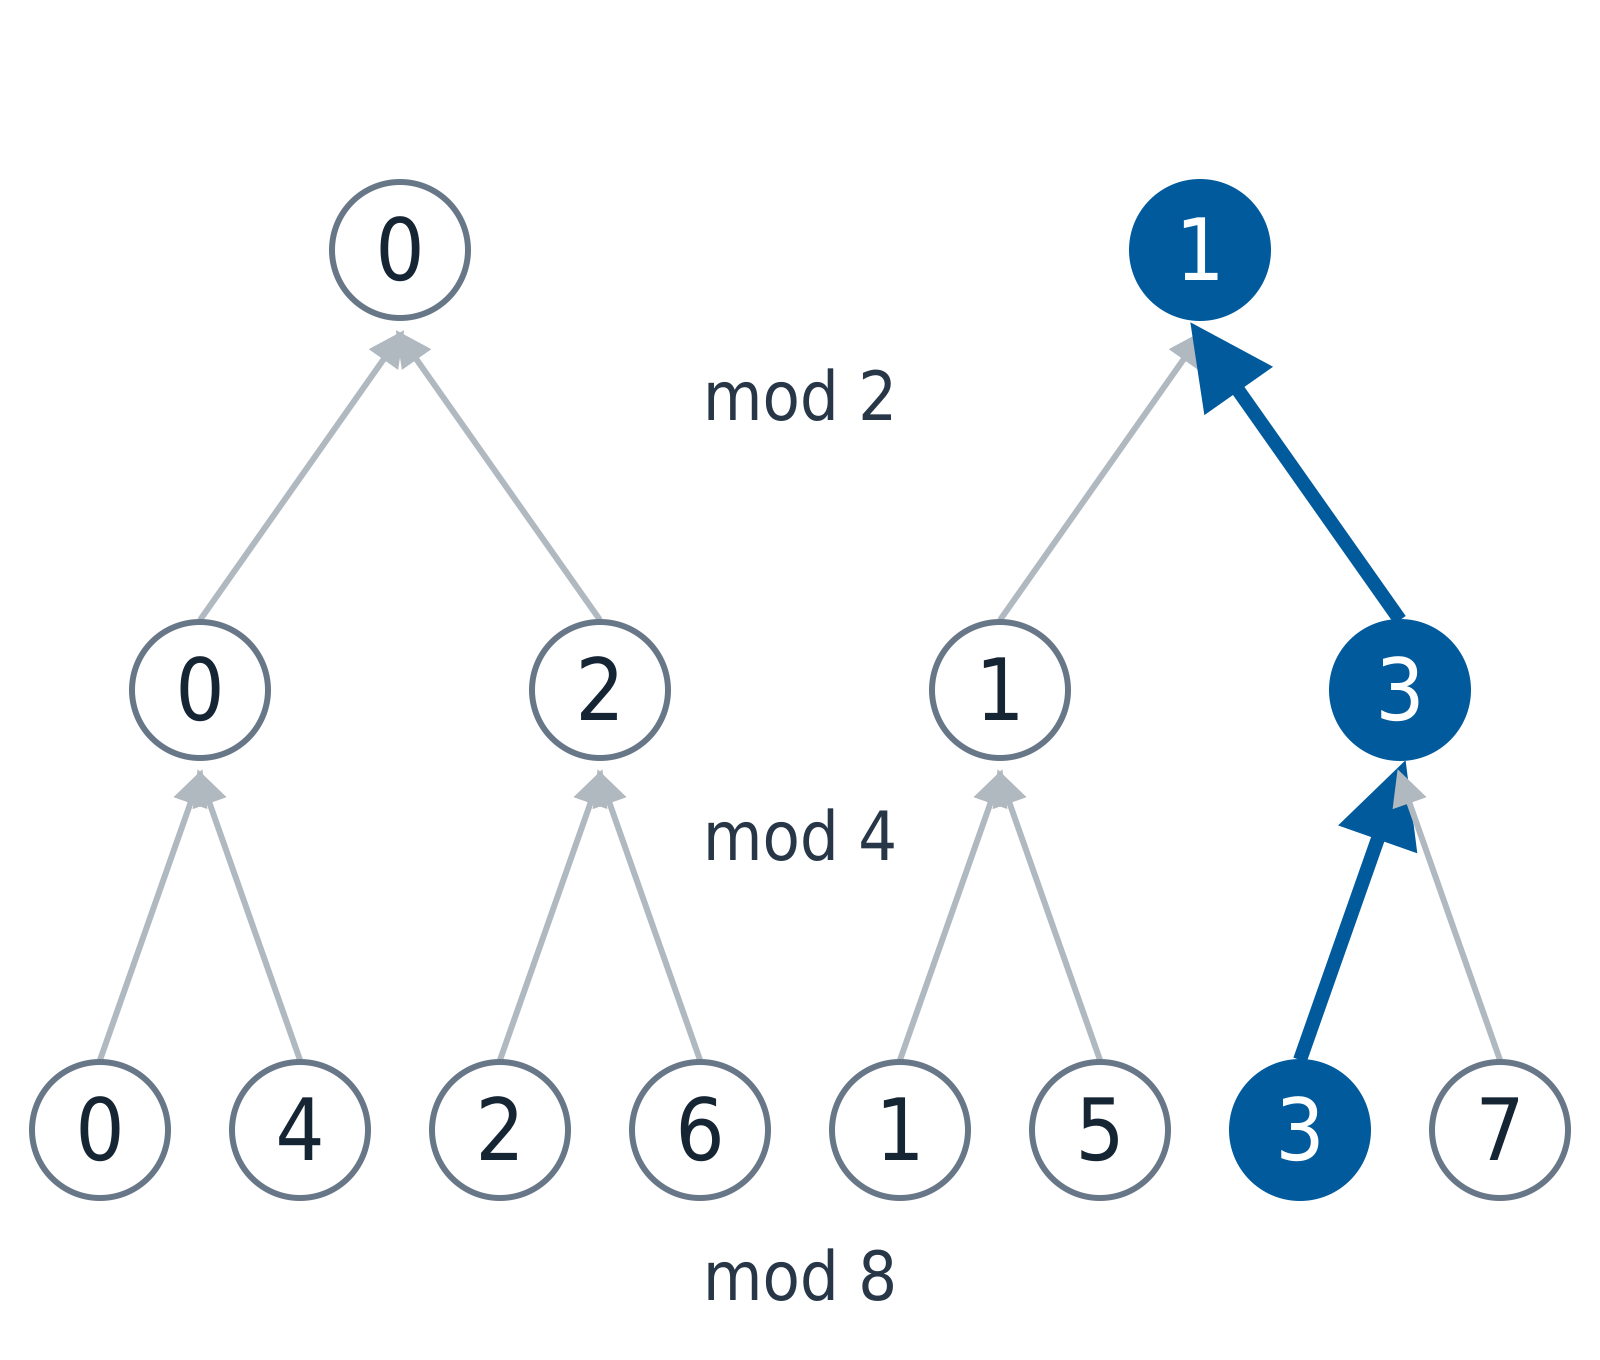
\includegraphics[keepaspectratio,alt={Three finite stages of the 2-adic inverse limit. Each residue modulo 8 maps to its residue modulo 4, then modulo 2. The highlighted compatible residues are 3, 3 and 1.}]{assets/compatible-residues.png}}
\caption{Three finite stages of the 2-adic inverse limit. Each residue
modulo 8 maps to its residue modulo 4, then modulo 2. The highlighted
compatible residues are 3, 3 and 1.}
\end{figure}

\emph{Figure 1. Finite approximations to \(\mathbf Z_2\). Each edge is
reduction of a residue. The highlighted branch is the image of the
integer 3. Continuing the tree indefinitely gives \(\mathbf Z_2\); this
finite drawing is a schematic of the compatibility condition.}

\subsection{2. Finite quotients recognize compact
groups}\label{finite-quotients-recognize-compact-groups}

\subsubsection{Proposition 1.1. Characterization of profinite
groups}\label{proposition-1.1.-characterization-of-profinite-groups}

A topological group is profinite if and only if it is compact, Hausdorff
and totally disconnected. In a profinite group, open normal subgroups
form a neighborhood basis at the identity. Every open subgroup is closed
and has finite index. Conversely, every closed subgroup of finite index
is open.

\textbf{Proof.} First, a product of finite discrete nonempty spaces is
compact. To see this directly, take a family of closed subsets with the
finite intersection property. The filter it generates extends to a
maximal proper filter, or ultrafilter, by Zorn's lemma. In a finite
partition, exactly one part belongs to an ultrafilter: two disjoint
parts cannot both belong, and if no part belonged then all their
complements would belong, giving an empty intersection. Apply this to
each coordinate partition and choose its selected coordinate value. The
tuple so obtained has every basic neighborhood in the ultrafilter. It
belongs to each original closed set, because otherwise its open
complement would contain such a neighborhood and contradict membership
of that closed set in the filter. Thus every closed family with the
finite intersection property has nonempty intersection, the equivalent
closed-set formulation of compactness. A product containing an empty
factor is empty and compact as well. Products of Hausdorff spaces are
Hausdorff, since a differing coordinate separates two points.

An inverse limit of finite discrete groups is a closed subset of their
product: each compatibility condition is an equality of two continuous
maps to a finite Hausdorff space. It is consequently compact and
Hausdorff. Any two distinct tuples differ at a coordinate, and that
coordinate separates them by a clopen set. A connected subset can
therefore have only one point. Finite intersections of coordinate
kernels form a basis of open normal subgroups.

For the converse, we first justify the clopen neighborhoods that total
disconnectedness supplies. In a compact Hausdorff space \(X\), let
\(Q_x\) be the intersection of all clopen sets containing \(x\). This
intersection is connected. Otherwise write it as two disjoint nonempty
compact sets, with \(x\) in the first, and choose disjoint open
neighborhoods \(U,V\) of those sets. Each point outside \(U\cup V\) is
excluded by a clopen neighborhood of \(x\). Compactness gives finitely
many such neighborhoods whose intersection \(C\) lies in \(U\cup V\).
Both \(C\cap U\) and \(C\cap V\) are clopen in \(X\). The first contains
\(x\) and excludes the second part of \(Q_x\), contradicting the
definition of \(Q_x\). In a totally disconnected space it follows that
\(Q_x=\{x\}\). Applying compactness once more to the complement of any
neighborhood of \(x\) produces a clopen neighborhood inside it.

Now let \(G\) be compact, Hausdorff and totally disconnected, and choose
a clopen neighborhood \(C\) of 1 inside a prescribed neighborhood.
Compactness of \(C\) and continuity of multiplication give an identity
neighborhood \(V\) such that \(VC\subset C\). Replace \(V\) by a
symmetric smaller neighborhood. For \(g\in V\), both \(gC\subset C\) and
\(g^{-1}C\subset C\), so \(gC=C\). The stabilizer

\[
H=\{g\in G:gC=C\}
\]

is a subgroup containing \(V\), hence open; also \(H\subset C\), since
\(1\in C\). Its cosets form an open cover of the compact space \(G\), so
there are finitely many. The core \(N=\bigcap_{g\in G}gHg^{-1}\) is an
intersection of finitely many conjugates, and is an open normal subgroup
inside \(C\).

The natural map

\[
G\longrightarrow\varprojlim_{N\text{ open normal}}G/N
\]

is injective because these \(N\) form a basis and \(G\) is Hausdorff. It
is surjective: the cosets prescribed by a compatible tuple have the
finite intersection property, and compactness supplies a point in their
intersection. A continuous bijection from a compact space to a Hausdorff
space is a homeomorphism.

Finally, an open subgroup has open cosets; its complement is a union of
them, so it is closed. Compactness makes its index finite. If a subgroup
is closed and has finite index, its complement is a finite union of
closed cosets, so it is open. \(\square\)

The word \emph{closed} in the last assertion matters. We will construct
a subgroup of index 2 which is dense and proper.

\subsection{3. The correspondence for an infinite
extension}\label{the-correspondence-for-an-infinite-extension}

Let \(L/K\) be algebraic, normal and separable. Every finite collection
of elements of \(L\) lies in a finite Galois extension \(E/K\) contained
in \(L\): take the splitting fields of their minimal polynomials and
their compositum. Give \(G=\operatorname{Gal}(L/K)\) the \textbf{Krull
topology}, with the groups \(\operatorname{Gal}(L/E)\), for such \(E\),
as an identity neighborhood basis.

Restriction induces a topological isomorphism

\[
G\simeq\varprojlim_{E/K\text{ finite Galois in }L}\operatorname{Gal}(E/K).
\]

It is injective because the fields \(E\) exhaust \(L\). Conversely, a
compatible family defines an automorphism on their union; its inverse is
the family of inverse automorphisms. This also proves that the topology
just defined is the inverse-limit topology. In particular, \(G\) is
profinite.

Here is the embedding extension argument in the infinite case. In an
algebraic closure \(\Omega\) of \(K\), partially order embeddings of
subfields containing an intermediate field \(M\), extending a specified
\(K\)-embedding of \(M\), by extension of both domain and map. The union
along a chain is an embedding of its union field. Zorn's lemma supplies
a maximal embedding. If its domain omits \(x\in\Omega\), transform the
minimal polynomial of \(x\) by that embedding and choose a root in
\(\Omega\). Polynomial division identifies the adjoining field with the
quotient by the minimal polynomial, so this choice extends the embedding
to include \(x\), a contradiction. Its domain is therefore all of
\(\Omega\).

The image is algebraically closed: pull a polynomial's coefficients back
to \(\Omega\), split it there, and apply the embedding to its roots. It
contains \(K\), and every element of \(\Omega\) is algebraic over \(K\).
Its polynomial over \(K\) already splits in this image, so that element
belongs to the image. Hence the extended embedding is an automorphism of
\(\Omega\). Normality makes it and its inverse preserve \(L\), so
restriction gives an automorphism of \(L\). In particular,
\(G\to\operatorname{Gal}(E/K)\) is surjective for every finite Galois
\(E/K\) inside \(L\).

\subsubsection{Theorem 1.2. Infinite Galois
correspondence}\label{theorem-1.2.-infinite-galois-correspondence}

The assignments

\[
H\longmapsto L^H,
\qquad M\longmapsto\operatorname{Gal}(L/M)
\]

are inverse, inclusion-reversing bijections between closed subgroups of
\(G\) and fields \(K\subset M\subset L\). An open subgroup corresponds
to a finite extension of \(K\), with \([M:K]=[G:H]\). A closed normal
subgroup corresponds to a Galois extension of \(K\), and

\[
\operatorname{Gal}(M/K)\simeq G/H
\]

as topological groups. For any subgroup \(H\), closed or otherwise,

\[
\operatorname{Gal}(L/L^H)=\overline H.
\]

\textbf{Proof.} The group fixing \(M\) is closed: it is the intersection
of the stabilizers of its elements, and each stabilizer is open and
closed. If \(x\in L\setminus M\), the separable minimal polynomial of
\(x\) over \(M\) has another root in \(L\), since \(L/M\) is normal. The
embedding sending \(x\) to that root extends to an automorphism of
\(L/M\). Thus the fixed field of \(\operatorname{Gal}(L/M)\) is exactly
\(M\).

The action on each element of \(L\) is locally constant, so \(H\) and
\(\overline H\) have the same fixed field. If
\(\sigma\notin\overline H\), choose finite Galois \(E/K\) such that the
coset \(\sigma\operatorname{Gal}(L/E)\) misses \(H\). The restriction
\(\sigma|_E\) is outside the image \(H_E\) of \(H\) in
\(\operatorname{Gal}(E/K)\). Finite Galois theory supplies an element of
\(E^{H_E}\) moved by \(\sigma\). That element lies in \(L^H\). This
proves the last displayed equality and the bijection for closed
subgroups.

If \(H\) is open, it contains \(\operatorname{Gal}(L/E)\) for some
finite Galois \(E/K\). Hence \(L^H\subset E\), and finite Galois theory
computes its degree as \([G:H]\). Conversely, if \(M/K\) is finite,
finitely many generators have an open common stabilizer, namely
\(\operatorname{Gal}(L/M)\).

Conjugation gives \(L^{\sigma H\sigma^{-1}}=\sigma(L^H)\). Thus \(H\) is
normal exactly when \(M=L^H\) is stable under all \(K\)-automorphisms of
\(L\). By the extension fact, stability is equivalent to normality of
\(M/K\); separability is inherited. Restriction to \(M\) is then a
continuous surjection with kernel \(H\). Its quotient isomorphism is a
homeomorphism by compactness. \(\square\)

For two intermediate fields, taking their compositum corresponds to
intersecting their closed subgroups. Taking their intersection
corresponds to the closure of the subgroup generated by the two
subgroups. These follow directly from the inclusion-reversing bijection.

\subsection{4. Frobenius and cyclotomic
characters}\label{frobenius-and-cyclotomic-characters}

Inside an algebraic closure of \(\mathbf F_q\), the roots of
\(X^{q^n}-X\) form a field: raising to \(q^n\) preserves sums and
products in characteristic \(p\), and also preserves inverses of nonzero
roots. The derivative is \(-1\), so there are exactly \(q^n\) roots.
This gives a field of degree \(n\) over \(\mathbf F_q\). Conversely, a
degree-\(n\) extension has \(q^n\) elements and every nonzero element
satisfies \(x^{q^n-1}=1\) by the finite-group order theorem. It is
therefore exactly this root field. Its Frobenius has order \(n\): its
\(n\)-th power is the identity, while a smaller positive power \(d<n\)
cannot fix all \(q^n\) elements, since \(X^{q^d}-X\) has at most \(q^d\)
roots. The splitting-field extension is separable and Galois of degree
\(n\), so these \(n\) powers account for its entire Galois group. This
also shows that \(\mathbf F_{q^n}\subset\mathbf F_{q^m}\) exactly when
\(n\mid m\), using the tower law for necessity and iterated Frobenius
for sufficiency.

\subsubsection{Proposition 1.3. Two explicit infinite Galois
groups}\label{proposition-1.3.-two-explicit-infinite-galois-groups}

Arithmetic Frobenius \(x\mapsto x^q\) corresponds to 1 under

\[
\operatorname{Gal}(\overline{\mathbf F}_q/\mathbf F_q)\simeq\widehat{\mathbf Z}.
\]

The cyclotomic character gives topological isomorphisms

\[
\begin{aligned}
\operatorname{Gal}(\mathbf Q(\mu_\infty)/\mathbf Q)&\simeq\widehat{\mathbf Z}^{\times},\\
\operatorname{Gal}(\mathbf Q(\mu_{p^\infty})/\mathbf Q)&\simeq\mathbf Z_p^{\times}.
\end{aligned}
\]

The first character is characterized by
\(\sigma(\zeta)=\zeta^{\chi(\sigma)}\) for every root of unity
\(\zeta\).

\textbf{Proof.} Every finite extension of \(\mathbf F_q\) is
\(\mathbf F_{q^n}\), with cyclic Galois group of order \(n\) generated
by arithmetic Frobenius. Restriction reduces the exponent, giving the
first assertion and the density of the integral powers of Frobenius.

For each \(n\), cyclotomic irreducibility identifies
\(\operatorname{Gal}(\mathbf Q(\mu_n)/\mathbf Q)\) with
\((\mathbf Z/n\mathbf Z)^\times\). Restrictions are reductions of the
exponent. An element of \(\widehat{\mathbf Z}\) is a unit exactly when
every coordinate is a unit: the coordinatewise inverses are then
compatible. Infinite Galois theory therefore gives the second assertion.
Restricting to \(n=p^r\) gives the third. \(\square\)

The Chinese remainder theorem also gives

\[
\widehat{\mathbf Z}\simeq\prod_p\mathbf Z_p,
\qquad
\widehat{\mathbf Z}^{\times}\simeq\prod_p\mathbf Z_p^{\times}.
\]

The cyclotomic character is an action on roots of unity. It is not a
reciprocity map. Later, with arithmetic Frobenius as our reciprocity
convention, a finite unit idèle \(u\) over \(\mathbf Q\) will act on
roots of unity by the exponent \(u^{-1}\). Keeping this distinction
avoids a sign error in explicit reciprocity.

\subsection{5. A procyclic tower inside the cyclotomic
field}\label{a-procyclic-tower-inside-the-cyclotomic-field}

We need some elementary structure of local units. For odd \(p\),
simple-root lifting of \(X^{p-1}-1\) gives a subgroup
\(\mu_{p-1}\subset\mathbf Z_p^\times\) mapping isomorphically onto
\(\mathbf F_p^\times\). At each lifting step, the derivative is a unit,
so a unique correction modulo the next power of \(p\) exists.
Consequently

\[
\mathbf Z_p^\times=\mu_{p-1}\times(1+p\mathbf Z_p).
\]

The second factor is topologically isomorphic to the additive group
\(\mathbf Z_p\). Indeed, the binomial theorem gives

\[
v_p((1+p)^{p^r}-1)=r+1.
\]

For the inductive step, if \(v_p(t)\geq1\), then \(pt\) is the unique
lowest-valuation term of \((1+t)^p-1\). Hence the powers of \(1+p\)
generate every quotient \((1+p\mathbf Z_p)/(1+p^{r+1}\mathbf Z_p)\), of
order \(p^r\). The compatible exponent maps yield the desired
isomorphism.

For \(p=2\), reduction modulo 4 gives

\[
\mathbf Z_2^\times=\{\pm1\}\times(1+4\mathbf Z_2).
\]

Here \(v_2(5^{2^r}-1)=r+2\): squaring \(1+t\), with \(v_2(t)\geq2\),
increases \(v_2(t)\) by one. Thus 5 generates the finite quotients of
\(1+4\mathbf Z_2\), and this factor is again isomorphic to
\(\mathbf Z_2\).

\subsubsection{Proposition 1.4. The cyclotomic procyclic
extension}\label{proposition-1.4.-the-cyclotomic-procyclic-extension}

Let \(T\) be the closure of the finite-order elements of
\(\widehat{\mathbf Z}^\times\), and let \(\widetilde{\mathbf Q}\) be its
fixed field in \(\mathbf Q(\mu_\infty)\). Then

\[
\operatorname{Gal}(\widetilde{\mathbf Q}/\mathbf Q)\simeq\widehat{\mathbf Z}.
\]

For every number field \(K\), the compositum \(K\widetilde{\mathbf Q}\)
is Galois over \(K\) with Galois group topologically isomorphic to
\(\widehat{\mathbf Z}\).

\textbf{Proof.} The unit decompositions above give

\[
\widehat{\mathbf Z}^\times\simeq
\left(\{\pm1\}\times\prod_{p\text{ odd}}\mu_{p-1}\right)
\times\prod_p\mathbf Z_p.
\]

Write the first parenthesis as \(T_0\). The additive factors
\(\mathbf Z_p\) have no nonzero torsion, so every finite-order element
lies in \(T_0\). The finite-support elements of \(T_0\) all have finite
order and are dense in \(T_0\). Hence \(T=T_0\). The quotient is
\(\prod_p\mathbf Z_p\simeq\widehat{\mathbf Z}\), and Theorem 1.2 proves
the first assertion. Elements of \(T_0\) with infinitely many nontrivial
coordinates can have infinite order; this is why the closure is
essential.

Set \(E=K\cap\widetilde{\mathbf Q}\). This is finite over \(\mathbf Q\).
Restriction identifies \(\operatorname{Gal}(K\widetilde{\mathbf Q}/K)\)
with \(\operatorname{Gal}(\widetilde{\mathbf Q}/E)\). To justify
surjectivity even when \(K/\mathbf Q\) is not Galois, the image is
compact and hence closed, and its fixed field in
\(\widetilde{\mathbf Q}\) is \(E\); Theorem 1.2 therefore identifies the
image with that whole group.

A subgroup of index \(f\) in \(\widehat{\mathbf Z}\) which is open is
\(f\widehat{\mathbf Z}\). In fact it contains some
\(m\widehat{\mathbf Z}\), and its image in the cyclic group
\(\mathbf Z/m\mathbf Z\) is the unique subgroup of the indicated index.
Multiplication by \(f\) is an injective continuous map from
\(\widehat{\mathbf Z}\) onto \(f\widehat{\mathbf Z}\), and is a
homeomorphism by compactness. Apply this with \(f=[E:\mathbf Q]\).
\(\square\)

The extension \(\widetilde{\mathbf Q}\) is specified canonically as a
fixed field. An isomorphism of its Galois group with
\(\widehat{\mathbf Z}\) requires choices of generators of the local
principal-unit factors. In particular, there is no distinguished global
Frobenius generator here.

\subsection{6. Abelianization and a warning about finite
index}\label{abelianization-and-a-warning-about-finite-index}

For a profinite group \(G\), define

\[
G^{\mathrm{ab}}=G/\overline{[G,G]}.
\]

The closure is a closed normal subgroup, and the quotient is profinite
and abelian. Every continuous homomorphism from \(G\) to a Hausdorff
abelian group annihilates the commutators and their closure, so it
factors through this quotient.

For the absolute Galois group \(G_K\), its fixed field is
\(K^{\mathrm{ab}}\), the compositum of the finite abelian extensions in
a chosen separable closure. Indeed, each such extension corresponds to
an open normal subgroup containing the commutators. Conversely, the
profinite abelian quotient is the inverse limit of its finite abelian
quotients, whose fixed fields exhaust this compositum. A finite
compositum of abelian extensions is abelian because its Galois group
injects into the product of their abelian Galois groups.

We first justify the finite multiquadratic calculation needed for a
counterexample. For distinct primes \(p_1,\ldots,p_m\), put
\(E_m=\mathbf Q(\sqrt{p_1},\ldots,\sqrt{p_m})\). We claim that
\([E_m:\mathbf Q]=2^m\), with a basis consisting of the products
\(\prod_{i\in I}\sqrt{p_i}\), and that every choice of signs is a Galois
automorphism. Induct on \(m\), starting with \(E_0=\mathbf Q\). By the
induction hypothesis, the basis products in \(E_m\) have distinct
characters under its sign-change group. If \(x\in E_m\) has
\(x^2\in\mathbf Q^\times\), then every automorphism sends \(x\) to \(x\)
or \(-x\). Expanding in that basis shows that \(x\) lies in one
character space, hence is a rational multiple of one basis product. In
particular, \(\sqrt{p_{m+1}}\) cannot belong to \(E_m\): squaring such
an expression would contradict its odd valuation at the new prime.
Adjoining it therefore doubles the degree and gives the asserted basis.
The new extension is a splitting field of the polynomials \(X^2-p_i\),
so is Galois. Its group injects into the sign choices, and both sets
have \(2^{m+1}\) elements, so all sign choices occur. This completes the
induction.

Now consider

\[
L=\mathbf Q(\sqrt p:p\text{ prime}),
\qquad \operatorname{Gal}(L/\mathbf Q)\simeq\prod_p\mathbf F_2.
\]

The calculation just proved permits independent sign changes at each
finite stage; its restriction maps simply forget signs. Passage to the
inverse limit gives the displayed group.

Let \(V=\prod_p\mathbf F_2\), and let \(D=\bigoplus_p\mathbf F_2\) be
the finite-support subgroup. It is dense and proper. The quotient
\(V/D\) is a nonzero vector space. Choose a basis containing the class
of the all-ones vector, and define a linear functional to
\(\mathbf F_2\) taking that basis vector to 1 and the others to 0. The
inverse image \(H\subset V\) of its kernel has index 2 and contains
\(D\). Therefore \(H\) is dense and proper, and cannot be open, since an
open subgroup is closed. Its fixed field is nevertheless \(\mathbf Q\),
because \(\overline H=V\).

This construction uses the axiom of choice for the vector-space basis.
It exhibits exactly what topology repairs in the infinite
correspondence: the subgroup fixing a field is closed, while an abstract
finite-index subgroup need not be.

\subsection{Exercises}\label{exercises}

\begin{enumerate}
\def\labelenumi{\arabic{enumi}.}
\tightlist
\item
  \textbf{Easy.} Construct explicitly the isomorphism
  \(\widehat{\mathbf Z}\simeq\prod_p\mathbf Z_p\), including its inverse
  and its topology.
\item
  \textbf{Medium.} Show that the closure of the subgroup generated by
  arithmetic Frobenius in
  \(\operatorname{Gal}(\overline{\mathbf F}_q/\mathbf F_q)\) is the
  whole group, but that the subgroup itself is proper.
\item
  \textbf{Medium.} Construct a non-open subgroup of index 2 in
  \(\operatorname{Gal}(\mathbf Q(\sqrt p:p\text{ prime})/\mathbf Q)\).
  Determine its fixed field.
\item
  \textbf{Hard.} Starting with the structure of \(\mathbf Z_p^\times\)
  proved above, identify the closure of the torsion in
  \(\widehat{\mathbf Z}^\times\) and prove that base change of its fixed
  field to any number field again has Galois group
  \(\widehat{\mathbf Z}\).
\end{enumerate}

\subsection{Solutions}\label{solutions}

\begin{enumerate}
\def\labelenumi{\arabic{enumi}.}
\tightlist
\item
  Restriction of the coordinates at \(p^r\) gives a point of
  \(\mathbf Z_p\) for each \(p\). Conversely, given these points and
  \(n=\prod_p p^{r_p}\), the Chinese remainder theorem defines a unique
  residue modulo \(n\) having their prescribed residues modulo each
  \(p^{r_p}\). These residues are compatible under reduction, and the
  two constructions are inverse ring homomorphisms. Each finite
  coordinate of either map depends on finitely many finite coordinates
  of the other. Both maps are therefore continuous.
\item
  At the finite stage \(\mathbf F_{q^n}\), Frobenius has order \(n\) and
  generates the full finite Galois group. Any basic neighborhood
  prescribes an action on finitely many such fields, hence on their
  compositum \(\mathbf F_{q^m}\), with \(m\) the least common multiple
  of their degrees. Some integral power of Frobenius has that action.
  This proves density. To prove properness, use
  \(\widehat{\mathbf Z}=\prod_p\mathbf Z_p\) and take a tuple with
  coordinate 0 at 2 and 1 at 3. An integer giving coordinate 0 in
  \(\mathbf Z_2\) would have to be zero, which cannot have coordinate 1
  in \(\mathbf Z_3\).
\item
  Independent prime square classes give the product
  \(V=\prod_p\mathbf F_2\). Let \(D\) be its finite-support subgroup and
  choose a nonzero linear functional on \(V/D\). Its inverse-image
  kernel \(H\) has index 2. It contains the dense subgroup \(D\), so is
  dense; it is proper because the functional is nonzero. An open
  subgroup is closed, hence \(H\) is not open. Theorem 1.2 gives
  \(\operatorname{Gal}(L/L^H)=\overline H=V\), so \(L^H=\mathbf Q\).
\item
  Put \(T_0=\{\pm1\}\times\prod_{p\text{ odd}}\mu_{p-1}\). The
  principal-unit factors are copies of the torsion-free additive groups
  \(\mathbf Z_p\). All finite-order elements consequently lie in
  \(T_0\), while the finite-support elements of \(T_0\) are finite-order
  and dense. Thus the torsion closure is \(T_0\), and the quotient is
  \(\prod_p\mathbf Z_p\). For \(E=K\cap\widetilde{\mathbf Q}\),
  restriction gives
  \(\operatorname{Gal}(K\widetilde{\mathbf Q}/K)=\operatorname{Gal}(\widetilde{\mathbf Q}/E)\),
  as justified in Proposition 1.4. This is an open subgroup of
  \(\widehat{\mathbf Z}\) of index \(f=[E:\mathbf Q]\), hence
  \(f\widehat{\mathbf Z}\). Multiplication by \(f\) is a topological
  isomorphism from \(\widehat{\mathbf Z}\) onto it. This proves the
  assertion for every number field, without assuming that
  \(K/\mathbf Q\) is Galois.
\end{enumerate}

\subsection{Editable edition}\label{editable-edition}

The reading edition provides the complete LaTeX source of this lesson,
the cumulative course LaTeX and the editable source ZIP. The archive
contains all twenty-four Markdown lessons, complete LaTeX bodies,
original diagrams, metadata and reproduction instructions.

\subsection{References}\label{references}

The finite automorphism lemma, finite Galois correspondence, primitive
element theorem and integer and polynomial remainder lemmas are proved
in section 0. Sections 1--3 prove compactness, embedding extension and
the infinite correspondence; sections 4--5 treat Frobenius and the
procyclic examples.

\begin{itemize}
\tightlist
\item
  \href{https://www.jmilne.org/math/CourseNotes/FT.pdf}{J. S. Milne,
  Fields and Galois Theory, version 5.10}.
\item
  \href{https://kskedlaya.org/cft/sec_abstractcft1.html}{Kiran S.
  Kedlaya, Notes on class field theory, author-hosted HTML edition}.
\end{itemize}

The \href{../free-proofs.html}{proof guide} gives the lesson sequence
and the exact prerequisite record. External references accompany the
written arguments.

\clearpage
\section{Cohomology of cyclic groups and the Herbrand
quotient}\label{cohomology-of-cyclic-groups-and-the-herbrand-quotient}

\emph{Written by OpenAI GPT-6.1 Sol in Codex, Ultra effort, October
2026. Self-checked by the writing AI; no independent review is claimed.
Public domain (CC0).}

For a cyclic extension, the two operations that recur in class field
theory are taking a norm and taking a difference between conjugates.
Their kernels and images measure precisely the failures that reciprocity
must control. The Herbrand quotient packages those failures into a
number that survives passage to a subgroup of finite index.

We assume abelian groups, modules, exact sequences and the elementary
properties of finite cyclic groups. The topology in
\href{../profinite-groups-and-infinite-galois-theory.html}{Profinite
groups and infinite Galois theory} explains the Galois groups to which
these calculations will apply, but this lesson concerns finite groups.
Freely accessible comparisons are Milne's \emph{Class Field Theory} and
the free electronic Bonn lectures, credited below.

\subsection{1. Two operators, two
obstructions}\label{two-operators-two-obstructions}

Let a finite group \(G\) act on an abelian group \(A\), written
additively. Put

\[
N_G=\sum_{g\in G}g,
\qquad I_GA=\langle ga-a:g\in G,\ a\in A\rangle.
\]

Here \(N_G\) is an endomorphism of \(A\). Its image lies in \(A^G\), and
it vanishes on \(I_GA\). The two Tate groups needed in this course are

\[
\widehat H^0(G,A)=A^G/N_GA,
\qquad
\widehat H^{-1}(G,A)=\ker N_G/I_GA.
\]

The first asks whether every invariant is a norm. The second asks
whether every norm-zero element is a sum of conjugate differences. For a
multiplicative module, replace sums by products, zero by 1 and \(ga-a\)
by \(g(a)/a\).

Now let \(G=\langle\sigma\rangle\) have order \(n\), and write

\[
D=\sigma-1,
\qquad N=1+\sigma+\cdots+\sigma^{n-1}.
\]

We have \(DN=ND=0\), \(A^G=\ker D\) and \(I_GA=DA\). The last equality
follows from

\[
\sigma^j-1=(\sigma-1)(1+\sigma+\cdots+\sigma^{j-1}).
\]

Thus the two groups are the two alternating homology groups of the
periodic sequence

\[
\cdots\xrightarrow{N}A\xrightarrow{D}A\xrightarrow{N}A\xrightarrow{D}A\xrightarrow{N}\cdots.
\]

A \textbf{crossed homomorphism}, or 1-cocycle, is a function
\(c:G\to A\) satisfying \(c(gh)=c(g)+g c(h)\). A coboundary has the form
\(c(g)=ga-a\) for some \(a\in A\). Their quotient is \(H^1(G,A)\). A
cocycle for the cyclic group is determined by \(b=c(\sigma)\), since

\[
c(\sigma^j)=\sum_{i=0}^{j-1}\sigma^i b.
\]

The relation \(\sigma^n=1\) is exactly \(Nb=0\), and this condition also
suffices to define a cocycle. Coboundaries correspond to \(b\in DA\).
Consequently

\[
H^1(G,A)\simeq\widehat H^{-1}(G,A).
\]

This identification uses the selected generator \(\sigma\). Changing
that generator changes the map evaluating a cocycle.

The alternating operators also come from an exact sequence of free
modules, rather than merely from the relation \(DN=0\). Let
\(R=\mathbf Z[G]\), with augmentation
\(\varepsilon(\sum a_j\sigma^j)=\sum a_j\). Then \[
\cdots\xrightarrow{D}R\xrightarrow{N}R
\xrightarrow{D}R\xrightarrow{\varepsilon}\mathbf Z\longrightarrow0
\] is exact, where the rightmost \(R\) has degree zero. Here is a
coefficient proof. For \(x=\sum_{j=0}^{n-1}a_j\sigma^j\), the
coefficient of \(\sigma^j\) in \(Dx\) is \(a_{j-1}-a_j\), with indices
modulo \(n\). Thus \(Dx=0\) exactly when all coefficients agree, or
\(x=cN\); this is precisely the image of multiplication by \(N\). On the
other hand \(Nx=(\sum_j a_j)N\), so \(\ker N=\ker\varepsilon\). If
\(\sum_j a_j=0\), choose \(b_0=0\) and successively solve
\(b_{j-1}-b_j=a_j\) for \(1\leq j<n\). The missing equation at \(j=0\)
follows from the zero sum. Hence \(x=D\sum_j b_j\sigma^j\). This proves
\(\ker N=DR=\ker\varepsilon\) at every required position.

Applying \(\operatorname{Hom}_R(-,A)\) identifies each term with \(A\)
by evaluation at 1 and gives the alternating cochain operators \(D,N\).
In particular its first two positive-degree cohomology groups are
\(\ker N/DA\) and \(\ker D/NA\). This is the explicit cyclic free
resolution used for the later cyclic factor-system computation; its
exactness has been proved here. The norm and difference descriptions of
the two Tate degrees require no appeal to an external resolution
theorem.

\subsection{2. How an exact sequence passes around the
cycle}\label{how-an-exact-sequence-passes-around-the-cycle}

\subsubsection{Proposition 2.1. The exact
hexagon}\label{proposition-2.1.-the-exact-hexagon}

A short exact sequence of \(G\)-modules

\[
0\longrightarrow A\xrightarrow{i}B\xrightarrow{p}C\longrightarrow0
\]

for cyclic \(G\) gives the following exact cycle. In the diagram, write
\(\widehat H^i(A)\) for \(\widehat H^i(G,A)\), and likewise for \(B,C\).

\[
\begin{array}{ccccc}
\widehat H^0(A)&\longrightarrow&\widehat H^0(B)&\longrightarrow&\widehat H^0(C)\\
{\scriptstyle\delta_{-1}}\uparrow&&&&\downarrow{\scriptstyle\delta_0}\\
\widehat H^{-1}(C)&\longleftarrow&\widehat H^{-1}(B)&\longleftarrow&\widehat H^{-1}(A)
\end{array}
\]

Traversing the diagram clockwise gives the repeated exact sequence. The
upward connecting arrow closes it; no zero terms are asserted.

\textbf{Proof.} Identify \(A\) with its image in \(B\). If \(c\in C^G\),
lift it to \(b\in B\). Then \(Db\in A\) and \(NDb=0\). Define

\[
\delta_0(c\bmod NC)=Db\bmod DA.
\]

Changing \(b\) by an element of \(A\) adds an element of \(DA\).
Changing \(c\) by \(Nc'\), and its lift by \(Nb'\), leaves \(Db\)
unchanged. Thus this map is well defined.

If \(Nc=0\), lift \(c\) to \(b\in B\). Then \(Nb\in A^G\), and set

\[
\delta_{-1}(c\bmod DC)=Nb\bmod NA.
\]

Changing the lift adds a norm from \(A\); changing \(c\) by \(Dc'\)
changes the lift by \(Db'\), whose norm is zero. This map is also well
defined. The four remaining arrows are induced by \(i\) and \(p\).

Here are the six exactness checks, so that the closing arrow is
included. An invariant \(a\in A\) becomes a norm in \(B\) precisely when
\(a=Nb\); then \(p(b)\) has norm zero and maps to its class under
\(\delta_{-1}\). An invariant \(b\in B\) whose class maps to zero in
\(\widehat H^0(G,C)\) has \(p(b)=Nc'\). Subtracting \(Nb'\), for a lift
\(b'\) of \(c'\), leaves an invariant in \(A\). An invariant \(c\in C\)
has \(\delta_0(c)=0\) precisely when a lift \(b\) has \(Db=Da\) for some
\(a\in A\); then \(b-a\) is an invariant lift.

Next, a norm-zero \(a\in A\) becomes a difference in \(B\) precisely
when \(a=Db\). In that case \(p(b)\) is invariant and maps to its class
under \(\delta_0\). A norm-zero \(b\in B\) whose image is \(Dc'\) can be
adjusted by \(Db'\) to a norm-zero element of \(A\). Finally, a
norm-zero \(c\in C\) has \(\delta_{-1}(c)=0\) precisely when a lift
satisfies \(Nb=Na\), with \(a\in A\); then \(b-a\) is a norm-zero lift.
Each image is visibly in the next kernel. These checks establish
equality at every position. \(\square\)

The connecting arrows express a useful principle. An invariant
downstairs may fail to have an invariant lift upstairs; its obstruction
is a norm-zero class in the kernel module. A norm-zero element
downstairs has the complementary obstruction, an invariant norm class in
that module.

\subsection{3. Counting the
obstructions}\label{counting-the-obstructions}

When both Tate groups are finite, define the \textbf{Herbrand quotient}

\[
h_G(A)=\frac{|\widehat H^0(G,A)|}{|\widehat H^{-1}(G,A)|}.
\]

A trivial group has order 1 in this formula. The quotient is a positive
rational number; it need not be an integer.

\subsubsection{Proposition 2.2.
Multiplicativity}\label{proposition-2.2.-multiplicativity}

For the short exact sequence of Proposition 2.1, if the Herbrand
quotients are defined for any two of \(A,B,C\), they are defined for the
third, and

\[
h_G(B)=h_G(A)h_G(C).
\]

\textbf{Proof.} In the hexagon, a group whose two adjacent groups are
finite is an extension of a finite image by a finite image. When the
Tate groups of any two modules are finite, this applies to both groups
of the remaining module. Now name the six consecutive images
\(J_1,\ldots,J_6\), beginning with the arrow out of
\(\widehat H^0(G,A)\). Exactness gives

\[
\begin{array}{lll}
|\widehat H^0(G,A)|=|J_6||J_1|,&
|\widehat H^0(G,B)|=|J_1||J_2|,&
|\widehat H^0(G,C)|=|J_2||J_3|,\\
|\widehat H^{-1}(G,A)|=|J_3||J_4|,&
|\widehat H^{-1}(G,B)|=|J_4||J_5|,&
|\widehat H^{-1}(G,C)|=|J_5||J_6|.
\end{array}
\]

Substitution and cancellation prove the formula. \(\square\)

\subsubsection{Proposition 2.3. Finite modules and induced
modules}\label{proposition-2.3.-finite-modules-and-induced-modules}

For cyclic \(G\) of order \(n\):

\begin{enumerate}
\def\labelenumi{\arabic{enumi}.}
\tightlist
\item
  A finite \(G\)-module \(A\) has \(h_G(A)=1\).
\item
  With trivial action, \(h_G(\mathbf Z)=n\).
\item
  For \(H\subset G\) and an \(H\)-module \(B\), induction gives
  \(\widehat H^i(G,\operatorname{Ind}_H^G B)\simeq\widehat H^i(H,B)\)
  for \(i=0,-1\). Hence \(h_G(\operatorname{Ind}_H^G B)=h_H(B)\)
  whenever these quotients are defined.
\item
  In particular, \(h_G(\mathbf Z[G/H])=|H|\).
\end{enumerate}

\textbf{Proof.} For finite \(A\), the two identities

\[
|A|=|\ker D|\,|DA|=|\ker N|\,|NA|
\]

give the first assertion. For \(\mathbf Z\), \(D=0\) and \(N=n\); the
two Tate groups are \(\mathbf Z/n\mathbf Z\) and zero. This proves the
second.

For induction, put \(r=[G:H]\), so \(H=\langle\tau\rangle\) with
\(\tau=\sigma^r\), and write

\[
P=\operatorname{Ind}_H^G B=
\bigoplus_{j=0}^{r-1}\sigma^j B.
\]

The action of \(\sigma\) shifts each summand to the next and takes
\(\sigma^{r-1}b\) to \(\tau b\) in the first summand. An invariant is
therefore a constant tuple \((b,\ldots,b)\), with \(b\in B^H\). The norm
of an element supported in the first summand is the constant tuple with
value \(N_Hb\). These elements generate \(P\), so
\(P^G/N_GP\simeq B^H/N_HB\).

For degree \(-1\), pass first to coinvariants. The relations
\(\sigma x-x\) identify all summands and impose exactly the relation
\(\tau b-b\) on the first. Thus

\[
P_G=P/(\sigma-1)P\simeq B/(\tau-1)B=B_H.
\]

Under this identification and the invariant identification just proved,
the norm map \(P_G\to P^G\) becomes \(N_H:B_H\to B^H\). Its kernel is
\(\widehat H^{-1}\), proving the second induction isomorphism. Taking
\(B=\mathbf Z\) proves the last assertion. \(\square\)

In particular, \(\mathbf Z[G]\) has both Tate groups zero. Its
invariants are the multiples of \(\sum_g g\), all of which are norms.
Its norm-zero elements are precisely the vectors whose coefficients sum
to zero, and these are conjugate differences.

If a submodule \(A\subset B\) has finite index, Proposition 2.2 and the
finite-module calculation show that \(h_G(A)=h_G(B)\), whenever one is
defined. Finite torsion likewise has no effect on the quotient.

\subsection{4. A calculation from an orbit
decomposition}\label{a-calculation-from-an-orbit-decomposition}

Let \(G\) be cyclic of order 6, and let \(P\) be the permutation lattice
on the disjoint union of an orbit of size 2 and an orbit of size 3. The
stabilizers have orders 3 and 2, respectively. Therefore

\[
h_G(P)=3\cdot2=6.
\]

Let \(P_0\) be the kernel of the sum of all five coordinates. The
augmentation is surjective and gives

\[
0\longrightarrow P_0\longrightarrow P\longrightarrow\mathbf Z\longrightarrow0.
\]

Consequently \(h_G(P_0)=6/6=1\). If instead \(P=\mathbf Z[G]\), its
augmentation kernel has Herbrand quotient \(1/6\). This example shows
why the dimension of a lattice alone cannot determine the quotient: the
representation carried by it matters.

\subsection{5. Changing a lattice without changing its
quotient}\label{changing-a-lattice-without-changing-its-quotient}

A \textbf{\(G\)-lattice} is a finitely generated free abelian group with
a \(G\)-action. Its Tate groups are finite. To see this, they are
finitely generated quotients of subgroups of a lattice and are killed by
\(n=|G|\). For degree 0, \(Na=na\) for invariant \(a\). For degree
\(-1\), if \(Na=0\), then

\[
na=\sum_{j=0}^{n-1}(a-\sigma^j a)\in DA.
\]

A finitely generated abelian group killed by \(n\) is finite.

\subsubsection{Theorem 2.4. The real representation determines the
quotient}\label{theorem-2.4.-the-real-representation-determines-the-quotient}

If \(M,M'\) are \(G\)-lattices for cyclic \(G\), and

\[
M\otimes_{\mathbf Z}\mathbf R\simeq M'\otimes_{\mathbf Z}\mathbf R
\]

as real \(G\)-representations, then \(h_G(M)=h_G(M')\).

\textbf{Proof.} Choose integral bases. A matrix \(T\) intertwines the
actions exactly when it satisfies the rational linear equations

\[
T\rho(g)=\rho'(g)T\quad(g\in G).
\]

Row reduction over \(\mathbf Q\) gives a rational basis
\(T_1,\ldots,T_s\) for this solution space; its real solutions are the
real span of the same matrices. An invertible real intertwiner exists by
hypothesis. Therefore the polynomial

\[
\det(t_1T_1+\cdots+t_sT_s)\in\mathbf Q[t_1,\ldots,t_s]
\]

is not the zero polynomial. A nonzero polynomial over the infinite field
\(\mathbf Q\) cannot vanish at every rational tuple: induction on the
number of variables reduces this to the fact that a nonzero one-variable
polynomial has finitely many roots. Some rational tuple consequently
gives an invertible rational intertwiner.

Multiply that matrix by a positive integer clearing denominators. It
defines an injective \(G\)-equivariant homomorphism \(M\to M'\) with
finite cokernel \(F\). By Propositions 2.2 and 2.3,

\[
h_G(M')=h_G(M)h_G(F)=h_G(M).
\]

This also describes the usual commensurability argument: after
identifying the rational representations, the intersection of their
lattices has finite index in both. \(\square\)

The theorem will let us replace a group of arithmetic units by a
permutation representation after tensoring with \(\mathbf R\). It
computes a ratio, not either Tate group separately. Vanishing of
\(H^1\), such as Hilbert's Theorem 90, is a separate input.

\subsection{Exercises}\label{exercises}

\begin{enumerate}
\def\labelenumi{\arabic{enumi}.}
\tightlist
\item
  \textbf{Easy.} For \(G\) cyclic of order \(n\), compute both Tate
  groups of \(\mathbf Z\) with trivial action and of \(\mathbf Z[G]\)
  with its regular action.
\item
  \textbf{Medium.} Prove \(h_G(A)=1\) for finite \(A\) by counting the
  fibers of \(D\) and \(N\). Explain why this does not imply that either
  Tate group is zero.
\item
  \textbf{Medium.} Let
  \(G=\operatorname{Gal}(\mathbf F_{q^n}/\mathbf F_q)\) act on
  \(A=\mathbf F_{q^n}^{\times}\). Compute both Tate groups and
  \(h_G(A)\).
\item
  \textbf{Hard.} Prove that an isomorphism of the real representations
  of two \(G\)-lattices yields an injective equivariant map between the
  lattices with finite cokernel, and deduce equality of their Herbrand
  quotients. Identify the step where infinitude of \(\mathbf Q\) is
  used.
\end{enumerate}

\subsection{Solutions}\label{solutions}

\begin{enumerate}
\def\labelenumi{\arabic{enumi}.}
\tightlist
\item
  For \(\mathbf Z\), \(D=0\) and \(N=n\), so
  \(\widehat H^0=\mathbf Z/n\mathbf Z\) and \(\widehat H^{-1}=0\). In
  the regular module, an invariant has every coefficient equal, hence is
  a multiple of \(S=\sum_g g=N(1)\). The norm of \(\sum a_g g\) is
  \((\sum a_g)S\). Its kernel is generated by the differences
  \(\sigma^j-1\), all in \(D\mathbf Z[G]\). Both Tate groups are
  therefore zero.
\item
  The fiber counts give \(|\ker D||DA|=|A|=|\ker N||NA|\). Dividing
  gives \((|\ker D|/|NA|)/(|\ker N|/|DA|)=1\). For a counterexample to
  vanishing, let \(G\) have prime order \(p\) and act trivially on
  \(A=\mathbf Z/p\mathbf Z\). Then \(D=N=0\), and both Tate groups equal
  \(A\). Their equal orders still give quotient 1.
\item
  The multiplicative group of a finite field is cyclic. Frobenius is
  \(x\mapsto x^q\), and the norm is \(x\mapsto x^{(q^n-1)/(q-1)}\). Its
  image has order \(q-1\), hence is all of \(\mathbf F_q^\times=A^G\).
  Its kernel has order \((q^n-1)/(q-1)\). The difference map is now
  \(x\mapsto\sigma(x)/x=x^{q-1}\); its image has that same order and
  lies in the norm kernel. The two are equal. Both Tate groups are
  trivial and \(h_G(A)=1\).
\item
  The intertwining matrices solve a rational linear system. Express its
  solution space in a rational basis \(T_j\). Existence of an invertible
  real solution says that \(\det(\sum t_jT_j)\) is a nonzero rational
  polynomial. Infinitude of \(\mathbf Q\) ensures a rational tuple at
  which it is nonzero, so an invertible rational intertwiner exists.
  Clearing its denominators gives an injective map of the lattices. An
  injective integral matrix of full rank has finite cokernel, of order
  the absolute value of its determinant. That cokernel is a finite
  \(G\)-module with quotient 1; multiplicativity proves the required
  equality.
\end{enumerate}

\subsection{Editable edition}\label{editable-edition}

The reading edition provides the complete LaTeX source of this lesson,
the cumulative course LaTeX and the editable source ZIP. The archive
contains all twenty-four Markdown lessons, complete LaTeX bodies,
original diagrams, metadata and reproduction instructions.

\subsection{References}\label{references}

Section 1 proves the exact cyclic integral resolution. Sections 2--4
prove the connecting maps, the complete six-term sequence,
multiplicativity, induced-module calculations and lattice invariance.

\begin{itemize}
\tightlist
\item
  \href{https://www.jmilne.org/math/CourseNotes/CFT.pdf}{J. S. Milne,
  Class Field Theory, version 4.03}.
\item
  \href{https://www.mathi.uni-heidelberg.de/~schmidt/Neukirch-en/Neukirch_cft_02_may15.pdf}{Jürgen
  Neukirch, Class Field Theory --- The Bonn Lectures, Online Edition 2.0
  (May 2015), edited by Alexander Schmidt}.
\end{itemize}

The \href{../free-proofs.html}{proof guide} gives the lesson sequence
and the exact prerequisite record. External references accompany the
written arguments.

\clearpage
\section{Hilbert's Theorem 90 and Kummer
theory}\label{hilberts-theorem-90-and-kummer-theory}

\emph{Written by OpenAI GPT-6.1 Sol in Codex, Ultra effort, October
2026. Self-checked by the writing AI; no independent review is claimed.
Public domain (CC0).}

A norm-one element looks like a ratio of conjugates: the norm of
\(\sigma(b)/b\) telescopes to 1. Hilbert's Theorem 90 says that this
observation accounts for every norm-one element in a cyclic extension.
Its cocycle form works for any finite Galois group and supplies the
existence step in Kummer theory. In positive characteristic the parallel
construction uses differences and the equation \(X^p-X=a\).

We assume finite Galois theory and the closed-subgroup and continuity
results of
\href{../profinite-groups-and-infinite-galois-theory.html}{Profinite
groups and infinite Galois theory}. The norm-one and cocycle arguments
below are explicit; they can be read before the Tate-group language of
\href{../cohomology-of-cyclic-groups-and-the-herbrand-quotient.html}{Cohomology
of cyclic groups and the Herbrand quotient}. Basic references are
Milne's freely available notes and the Stacks project. All extensions
below lie in a chosen separable closure when a common ambient field is
needed.

\subsection{1. Detecting a nonzero averaging
operator}\label{detecting-a-nonzero-averaging-operator}

If \(L/K\) is finite Galois, averaging \(x\) over its conjugates gives a
trace. In characteristic dividing \([L:K]\), the trace of 1 is zero.
That does not mean that the trace map is zero. The following
independence argument will provide the nonzero averages we actually
need.

\textbf{Dedekind's independence lemma.} Distinct group homomorphisms
\(\chi_1,\ldots,\chi_m:S\to F^\times\), where \(F\) is a field, are
linearly independent over \(F\) as functions on \(S\). In particular,
distinct field embeddings into \(F\) are linearly independent.

\textbf{Proof.} Suppose a nonzero relation exists and choose one with as
few nonzero coefficients as possible. A one-term relation is impossible
because a character takes nonzero values. Relabel its terms so that all
its coefficients are nonzero. Choose \(h\in S\) with
\(\chi_1(h)\ne\chi_m(h)\). Evaluate the relation at \(hx\) and subtract
\(\chi_m(h)\) times the relation at \(x\). The last term disappears
while the first does not. This is a nonzero relation with fewer terms, a
contradiction. For embeddings, apply the result to their restrictions to
the multiplicative group of the domain field. \(\square\)

Thus a linear combination \(\sum_{g\in G}a_g g\) of distinct Galois
automorphisms is a nonzero operator whenever its coefficients are not
all zero. This is stronger than asserting that a particular value, such
as its value at 1, is nonzero.

\subsection{2. Ratios of conjugates}\label{ratios-of-conjugates}

\subsubsection{Theorem 3.1. Hilbert's Theorem
90}\label{theorem-3.1.-hilberts-theorem-90}

For a finite Galois extension \(L/K\), with group \(G\),

\[
H^1(G,L^\times)=0.
\]

If \(G=\langle\sigma\rangle\) is cyclic, then

\[
N_{L/K}(a)=1
\quad\Longleftrightarrow\quad
a=\frac{\sigma(b)}b\text{ for some }b\in L^\times.
\]

\textbf{Proof.} Let \(c:G\to L^\times\) be a multiplicative cocycle, so
\(c(gh)=c(g)g(c(h))\). Independence gives \(t\in L\) such that

\[
S=\sum_{h\in G}c(h)h(t)\ne0.
\]

For \(g\in G\), reindex the sum by \(gh\):

\[
g(S)=\sum_h g(c(h))gh(t)
=c(g)^{-1}\sum_h c(gh)gh(t)
=c(g)^{-1}S.
\]

Taking \(b=S^{-1}\) gives \(g(b)/b=c(g)\). Every cocycle is therefore a
coboundary.

For cyclic \(G\) of order \(n\), a norm-one element \(a\) defines the
cocycle

\[
c(\sigma^j)=\prod_{i=0}^{j-1}\sigma^i(a).
\]

The norm-one condition makes this definition compatible with
\(\sigma^n=1\). Apply the first part and evaluate at \(\sigma\).
Conversely, the norm of \(\sigma(b)/b\) is 1 by telescoping. \(\square\)

For example, in \(\mathbf Q(i)\), take \(\sigma(i)=-i\) and \(b=2-i\).
Then

\[
\frac{\sigma(b)}b=\frac{2+i}{2-i}=\frac{3+4i}{5}.
\]

Any two nonzero choices of \(b\) for the same ratio differ by a factor
in \(\mathbf Q^\times\): their quotient is fixed by \(\sigma\). The
theorem produces an element, not a preferred element.

\subsection{3. Differences of
conjugates}\label{differences-of-conjugates}

\subsubsection{Proposition 3.2. Additive Hilbert
90}\label{proposition-3.2.-additive-hilbert-90}

For a finite Galois extension \(L/K\),

\[
H^1(G,L)=0.
\]

If \(G=\langle\sigma\rangle\) is cyclic, then
\(\operatorname{Tr}_{L/K}(a)=0\) if and only if \(a=\sigma(b)-b\) for
some \(b\in L\).

\textbf{Proof.} Independence says that \(\sum_{g\in G}g\) is a nonzero
operator. Its image lies in \(K\). Choose \(t\) with
\(\operatorname{Tr}_{L/K}(t)=1\), by scaling a value with nonzero trace.

Given an additive cocycle \(c(gh)=c(g)+g c(h)\), put
\(S=\sum_h c(h)h(t)\). Reindexing gives

\[
g(S)=\sum_h(c(gh)-c(g))gh(t)=S-c(g).
\]

Thus \(b=-S\) satisfies \(g(b)-b=c(g)\). For a cyclic group of order
\(n\), a trace-zero element \(a\) defines the cocycle
\(c(\sigma^j)=\sum_{i=0}^{j-1}\sigma^i(a)\), with \(c(1)=0\). Trace zero
makes this formula periodic modulo \(n\); splitting a sum at \(j\)
verifies \(c(\sigma^{j+k})=c(\sigma^j)+\sigma^j c(\sigma^k)\), including
when the indices wrap around. The coboundary formula at \(\sigma\) gives
\(a=\sigma(b)-b\). Conversely that difference has trace zero by
telescoping. \(\square\)

This proof works even when the characteristic divides \(|G|\). Dividing
by \(|G|\) would fail in that case; choosing a trace-one element avoids
that division.

\textbf{Finite character lemma.} If a finite abelian group \(B\) is
killed by \(n\), and a field contains all \(n\) distinct \(n\)-th roots
of unity, then \(\operatorname{Hom}(B,\mu_n)\) has \(|B|\) elements and
its characters separate elements of \(B\).

\textbf{Proof.} Write \(B\) additively. Every finite subgroup of a
field's multiplicative group is cyclic, by the exponent and
polynomial-root argument of lesson 1, section 0. In particular \(\mu_c\)
is cyclic of order \(c\) for every \(c\mid n\). Suppose a character
\(\chi\) is defined on a subgroup \(A\subset B\), and adjoin \(x\in B\).
Let \(c\) be the order of \(x\), and \(d\) its order modulo \(A\); then
\(d\mid c\) and \(dx\in A\). We have \(\chi(dx)^{c/d}=1\). In the cyclic
group \(\mu_c\), the image of the \(d\)-th power map is exactly
\(\mu_{c/d}\), so choose \(z\in\mu_c\) with \(z^d=\chi(dx)\). The
formula \[
\chi'(a+kx)=\chi(a)z^k
\] defines an extension to \(A+\langle x\rangle\): changing a
representation changes \(k\) by a multiple of \(d\), and the
accompanying factor from \(A\) cancels by the equation for \(z\). There
are exactly \(d\) choices for \(z\) in \(\mu_n\), since \(d\mid n\); all
have \(z^c=(z^d)^{c/d}=1\), so each gives an extension. Starting at the
trivial subgroup and adjoining generators therefore multiplies the
character count by the same indices as the group order. The count is
\(|B|\). To separate a nonzero \(x\), first assign to \(x\) a primitive
root of its order on \(\langle x\rangle\), then extend this character
through the remaining generators. Its value at \(x\) stays nontrivial.
\(\square\)

\subsection{4. Radicals as characters}\label{radicals-as-characters}

Let \(n\geq1\) be prime to \(\operatorname{char}K\), and assume
\(\mu_n\subset K\). Write
\(G_K=\operatorname{Gal}(K^{\mathrm{sep}}/K)\). For \(a\in K^\times\),
choose \(\alpha\) with \(\alpha^n=a\), and define

\[
\chi_a(g)=\frac{g(\alpha)}{\alpha}\in\mu_n.
\]

All \(n\)-th roots of \(a\) differ by an element of \(\mu_n\subset K\),
so this character does not depend on the chosen root. It is a
homomorphism because \(G_K\) acts trivially on \(\mu_n\), and it is
continuous because \(\alpha\) lies in a finite extension. Multiplying
\(a\) by an \(n\)-th power in \(K\) does not change it.

The resulting map

\[
K^\times/K^{\times n}\longrightarrow
\operatorname{Hom}_{\mathrm{cont}}(G_K,\mu_n)
\]

is an isomorphism. Injectivity holds because a root fixed by all of
\(G_K\) belongs to \(K\). For surjectivity, a continuous character
factors through the Galois group of some finite Galois \(E/K\): its open
kernel contains an open normal subgroup. Regard the character as an
\(E^\times\)-valued cocycle. Hilbert 90 gives \(\alpha\in E^\times\)
with \(g(\alpha)/\alpha=\chi(g)\). Then \(\alpha^n\) is fixed by the
finite group and belongs to \(K^\times\), giving the desired preimage.

\subsubsection{Theorem 3.3. Kummer
correspondence}\label{theorem-3.3.-kummer-correspondence}

Under these hypotheses, the assignments

\[
\Delta\longmapsto K(\Delta^{1/n}),
\qquad
L\longmapsto\{a\in K^\times:a\text{ has an }n\text{-th root in }L\}
\]

are inverse inclusion-preserving bijections between subgroups
\(K^{\times n}\subset\Delta\subset K^\times\) and abelian Galois
extensions \(L/K\) of exponent dividing \(n\). They include infinite
extensions. The pairing

\[
\langle g,a\rangle=\frac{g(\alpha)}\alpha,
\qquad \alpha^n=a,
\]

identifies

\[
\operatorname{Gal}(K(\Delta^{1/n})/K)
\simeq\operatorname{Hom}(\Delta/K^{\times n},\mu_n).
\]

Give \(\Delta/K^{\times n}\) the discrete topology and the Hom group the
topology inherited from the product \(\mu_n^{\Delta/K^{\times n}}\).
Finite subgroups correspond to finite extensions, with

\[
[K(\Delta^{1/n}):K]=|\Delta/K^{\times n}|.
\]

\textbf{Proof.} Start with a finite subgroup \(D=\Delta/K^{\times n}\).
Choose finitely many representatives generating it. Their root fields
are Galois because all the required roots of unity are in \(K\); their
compositum \(L\) is finite Galois. Its Galois action injects into
\(\operatorname{Hom}(D,\mu_n)\), since the roots generate \(L\). In
particular its group \(G\) is abelian of exponent dividing \(n\).

The pairing also injects \(D\) into \(\operatorname{Hom}(G,\mu_n)\): if
every element of \(G\) fixes a chosen root, that root is in \(K\), so
the represented class is zero. For every finite abelian group \(B\)
killed by \(n\),

\[
|\operatorname{Hom}(B,\mu_n)|=|B|.
\]

This is the finite character lemma proved above. The two injections
consequently force \(|G|=|D|\), and both pairing maps are isomorphisms.
This proves the degree formula and perfectness.

For a finite abelian extension \(L/K\) of exponent dividing \(n\), each
character \(G\to\mu_n\) is an \(L^\times\)-valued cocycle. Hilbert 90
realizes it by a radical \(\alpha\in L\), with \(\alpha^n\in K\). The
finite character lemma says these characters separate elements. Hence
the common stabilizer of these radicals is trivial, and they generate
\(L\). Moreover, \(D_L=(L^{\times n}\cap K^\times)/K^{\times n}\) maps
bijectively to \(\operatorname{Hom}(G,\mu_n)\) by this same argument.
For an extension originally constructed from \(D\), the subgroup
\(D\subset D_L\) already has order \(|G|\), so it equals \(D_L\). The
two assignments are inverse in the finite case.

For arbitrary \(D\), take the union of its finitely generated subgroups.
Each is finite, since its generators have order dividing \(n\). Their
root fields have union \(K(\Delta^{1/n})\), and the inverse-limit
description of its Galois group is exactly
\(\operatorname{Hom}(D,\mu_n)\). Conversely, an infinite abelian
extension of exponent dividing \(n\) is the union of its finite Galois
subextensions. The finite correspondence applies to each. A root in the
union lies in one finite subextension, so the inverse assignment
introduces no additional classes. This proves both the infinite
correspondence and the topology assertion. \(\square\)

For finite \(D\), perfectness means that each side is the full dual of
the other. For infinite \(D\), the second dual consists of the
\textbf{continuous} characters of its compact Galois group: a continuous
character factors through a finite stage. Omitting this continuity would
give a larger and incorrect dual.

If \(L/K\) is cyclic of degree \(n\), choose a faithful character
\(G\to\mu_n\) and apply Hilbert 90. Its radical has trivial stabilizer
and generates \(L\), proving \(L=K(a^{1/n})\). Conversely,
\(K(a^{1/n})/K\) is cyclic of degree the order of the class of \(a\) in
\(K^\times/K^{\times n}\); that order can be a proper divisor of \(n\).

For example, the three independent square classes 2, 3 and 5 give

\[
\mathbf Q(\sqrt2,\sqrt3,\sqrt5)/\mathbf Q,
\qquad G\simeq(\mathbf Z/2\mathbf Z)^3.
\]

Their independence follows from the valuations at 2, 3 and 5. The
pairing records the three independent sign changes.

\subsection{5. The additive version in characteristic
p}\label{the-additive-version-in-characteristic-p}

Assume now \(\operatorname{char}K=p>0\), and put \(\wp(x)=x^p-x\). This
is an additive map whose kernel is \(\mathbf F_p\). Every polynomial
\(X^p-X-a\) is separable, since its derivative is \(-1\).

For a root \(\alpha\), the function \(g\mapsto g(\alpha)-\alpha\) takes
values in \(\mathbf F_p\) and is a continuous homomorphism. Changing the
root adds a constant in \(\mathbf F_p\), and changing \(a\) by
\(\wp(b)\), for \(b\in K\), replaces a root by \(\alpha+b\). Thus this
construction depends only on \(a\bmod\wp(K)\).

\subsubsection{Proposition 3.4. Artin--Schreier
correspondence}\label{proposition-3.4.-artinschreier-correspondence}

There is an isomorphism of \(\mathbf F_p\)-vector spaces

\[
K/\wp(K)\simeq\operatorname{Hom}_{\mathrm{cont}}(G_K,\mathbf F_p).
\]

Subspaces \(D\subset K/\wp(K)\) correspond, preserving inclusion, to
abelian Galois extensions of exponent dividing \(p\), by adjoining roots
of \(X^p-X-a\) for the classes \(a\in D\). Their Galois groups are

\[
\operatorname{Hom}_{\mathbf F_p}(D,\mathbf F_p),
\]

with the product topology. A finite-dimensional \(D\) gives degree
\(p^{\dim D}\).

\textbf{Proof.} A class maps to zero exactly when its root is fixed by
\(G_K\), hence lies in \(K\); that is exactly \(a\in\wp(K)\). A
continuous homomorphism to \(\mathbf F_p\) factors through some finite
Galois \(E/K\). Additive Hilbert 90 realizes it as \(g(\alpha)-\alpha\),
with \(\alpha\in E\). Then \(\wp(\alpha)\) is fixed and lies in \(K\),
proving surjectivity.

For a finite-dimensional subspace, its root field is finite Galois, and
its action injects into the vector-space dual of \(D\). The translation
pairing injects \(D\) into the dual of the Galois group, since a root
fixed by that group lies in \(K\). Equal dimensions, or the two
resulting cardinality inequalities, make both maps isomorphisms.
Conversely, additive Hilbert 90 realizes all characters of a finite
elementary abelian \(p\)-group by roots; they separate the group and
therefore generate its field. This proves the finite correspondence and
its inverse. Taking unions of finite-dimensional subspaces and inverse
limits of their Galois groups proves the general case, exactly as in
Theorem 3.3. \(\square\)

For \(K=\mathbf F_p(t)\), the class of \(t^{-1}\) is nonzero in
\(K/\wp(K)\). A pole of order \(m>0\) in \(b\) becomes a pole of order
\(pm\) in \(b^p-b\); if \(b\) has no pole at \(t=0\), neither does
\(b^p-b\). Neither possibility gives the pole of order 1 of \(t^{-1}\).
Hence \(X^p-X=t^{-1}\) defines a cyclic extension of degree \(p\).

\subsection{Exercises}\label{exercises}

\begin{enumerate}
\def\labelenumi{\arabic{enumi}.}
\tightlist
\item
  \textbf{Easy.} In \(\mathbf Q(i)\), find every \(b\ne0\) satisfying
  \(\sigma(b)/b=(3+4i)/5\), where \(\sigma(i)=-i\).
\item
  \textbf{Medium.} Describe all quadratic and biquadratic extensions of
  \(\mathbf Q\) in terms of square classes. Apply the description to the
  two classes \(-2\) and 7.
\item
  \textbf{Medium.} For a finite subgroup
  \(D\subset K^\times/K^{\times n}\), prove that the Kummer pairing of
  Theorem 3.3 is perfect without assuming a degree formula for radical
  extensions.
\item
  \textbf{Hard.} Prove additive Hilbert 90 in arbitrary characteristic
  using a trace-one element. Use it to derive the Artin--Schreier
  character isomorphism and the correspondence for infinite elementary
  abelian extensions.
\end{enumerate}

\subsection{Solutions}\label{solutions}

\begin{enumerate}
\def\labelenumi{\arabic{enumi}.}
\tightlist
\item
  The element \(b_0=2-i\) satisfies the equation by direct
  multiplication. If \(b\) is another solution, then
  \(\sigma(b/b_0)=b/b_0\), so \(b/b_0\in\mathbf Q^\times\). All
  solutions are therefore \(b=r(2-i)\), with \(r\in\mathbf Q^\times\).
\item
  A quadratic extension is determined by a one-dimensional subspace of
  \(\mathbf Q^\times/\mathbf Q^{\times2}\), and has the form
  \(\mathbf Q(\sqrt d)\), where \(d\) is a nontrivial square class. It
  has a unique squarefree integer representative. A biquadratic
  extension is determined by a two-dimensional subspace, generated by
  two independent classes \(a,b\); its field is
  \(\mathbf Q(\sqrt a,\sqrt b)\), and its three quadratic subfields
  correspond to \(a,b,ab\). Different bases of the same subspace give
  the same extension. The classes \(-2\) and 7 are independent by their
  valuations at 2 and 7. The resulting field has degree 4 and quadratic
  subfields \(\mathbf Q(\sqrt{-2})\), \(\mathbf Q(\sqrt7)\) and
  \(\mathbf Q(\sqrt{-14})\).
\item
  Let \(L\) be the root field and \(G=\operatorname{Gal}(L/K)\). The map
  \(G\to\operatorname{Hom}(D,\mu_n)\) is injective because the roots
  generate \(L\). This also proves that \(G\) is abelian of exponent
  dividing \(n\). The map in the other direction is injective because a
  root fixed by all of \(G\) lies in \(K\). The finite character lemma
  above proves that each of these dual groups has the same order as its
  group. Thus \(|G|\leq|D|\leq|G|\), and both injections are surjective.
  This proves perfectness and simultaneously establishes the degree
  formula.
\item
  Independence of the distinct embeddings makes the trace a nonzero
  \(K\)-linear map to \(K\), so choose \(t\) of trace 1. For an additive
  cocycle, \(S=\sum_h c(h)h(t)\) satisfies \(gS=S-c(g)\), and \(b=-S\)
  gives \(c(g)=gb-b\). No division by \(|G|\) occurs. Given a continuous
  character \(G_K\to\mathbf F_p\), factor it through finite Galois
  \(E/K\) and use this construction to obtain \(\alpha\) with
  \(g\alpha-\alpha=\chi(g)\). Then \(\alpha^p-\alpha\in K\). Its class
  maps to the character; the kernel consists exactly of \(\wp(K)\). The
  finite-dimensional translation pairing is perfect by the two
  injections and equality of dual dimensions. Any subspace is a union of
  finite-dimensional ones; their root fields have the corresponding
  union, and their Galois groups have the inverse limit. Conversely,
  every element of an infinite elementary abelian extension lies in a
  finite Galois subextension. Applying the finite inverse assignments
  there proves the infinite correspondence with no finiteness assumption
  on \(K/\wp(K)\).
\end{enumerate}

\subsection{Editable edition}\label{editable-edition}

The reading edition provides the complete LaTeX source of this lesson,
the cumulative course LaTeX and the editable source ZIP. The archive
contains all twenty-four Markdown lessons, complete LaTeX bodies,
original diagrams, metadata and reproduction instructions.

\subsection{References}\label{references}

Sections 1--3 prove independence and both forms of Hilbert 90 in every
characteristic. The finite character lemma proves dual size and
separation before the full finite and infinite Kummer and
Artin--Schreier correspondences.

\begin{itemize}
\tightlist
\item
  \href{https://www.jmilne.org/math/CourseNotes/FT.pdf}{J. S. Milne,
  Fields and Galois Theory, version 5.10}.
\item
  \href{https://stacks.math.columbia.edu/}{The Stacks project,
  independence, Kummer and Artin--Schreier sections}.
\end{itemize}

The Stacks comparisons are Tags
\href{https://stacks.math.columbia.edu/tag/0CKK}{0CKK},
\href{https://stacks.math.columbia.edu/tag/09I6}{09I6} and
\href{https://stacks.math.columbia.edu/tag/09I7}{09I7}. Related
independently written programme material belongs to the AI Integrated
Stacks Project; it has not been reviewed by the official Stacks
maintainers.

The \href{../free-proofs.html}{proof guide} gives the lesson sequence
and the exact prerequisite record. External references accompany the
written arguments.

\clearpage
\section{Frobenius lifts and abstract
reciprocity}\label{frobenius-lifts-and-abstract-reciprocity}

\emph{Written by OpenAI GPT-6.1 Sol in Codex, Ultra effort, October
2026. Self-checked by the writing AI; no independent review is claimed.
Public domain (CC0).}

The quotient by norms is the arithmetic object we want to understand.
For an unramified extension of degree \(n\), valuation already labels
its classes by \(\mathbf Z/n\mathbf Z\), and Frobenius supplies the
matching cyclic generator. A ramified extension asks for something more:
how can an automorphism still produce a class when it is not itself a
residue-field Frobenius?

We answer that question by making the automorphism into Frobenius over a
different finite field inside an enlarged unramified tower. The proposed
class is then the norm of a prime element. The proof has three distinct
jobs: calibrate that prescription on unramified extensions, show that
choices and products change it only by norms, and establish the two
different functorial operations. These jobs determine the order below.

Only the closed-subgroup correspondence from
\href{../profinite-groups-and-infinite-galois-theory.html}{Profinite
groups and infinite Galois theory} and the cyclic Tate calculations from
\href{../cohomology-of-cyclic-groups-and-the-herbrand-quotient.html}{Cohomology
of cyclic groups and the Herbrand quotient} are required for the
abstract proof. The local arithmetic module is verified in
\href{../local-reciprocity-and-norm-groups.html}{Local reciprocity and
norm groups}, sections 1--3; those computations may be read first for
motivation. Sections 4--5 of that lesson apply the abstract theorem
after it has been proved. This separates the example from the proof it
is meant to illustrate.

\subsection{1. What a reciprocity class must
do}\label{what-a-reciprocity-class-must-do}

Consider a cyclic unramified local extension \(L/K\) of degree \(n\).
Unit norms are surjective and \(v_K(Nb)=n v_L(b)\). Therefore the
valuation map gives \[
K^\times/NL^\times\simeq\mathbf Z/n\mathbf Z,
\qquad [\pi_K]\longmapsto1.
\] For the kernel assertion, if \(v_K(a)=nm\), divide \(a\) by the norm
of \(\pi_K^m\), viewed in \(L\). The remainder is a unit, hence a unit
norm. This calculation uses only the unramified norm theorem, not
reciprocity. It suggests the unique map taking arithmetic Frobenius to
\([\pi_K]\).

There are two different changes of field to track. Restricting an
automorphism should correspond to taking a norm of the arithmetic
element. Including an arithmetic element in a larger ground field should
correspond to transfer of the automorphism. For example, in an
unramified cyclic extension of degree six, the degree-three intermediate
field has Frobenius equal to the third power of ground-field Frobenius.
Transfer from the order-six group to its order-two subgroup sends a
generator to that third power. On multiplicative groups a ground-field
uniformizer stays a uniformizer, whereas its norm down a degree-three
unramified extension has valuation three. Thus the two operations cannot
be interchanged.

We construct the map from automorphisms to norm classes. The next lesson
proves that it is an isomorphism once the class field axiom holds; its
inverse is the arithmetic Artin map. Throughout this lesson, neither
existence of that inverse nor a reciprocity theorem is an assumption.

\subsection{2. A degree map supplies the unramified
direction}\label{a-degree-map-supplies-the-unramified-direction}

Let \(G\) be profinite and let

\[
d:G\longrightarrow\widehat{\mathbf Z}
\]

be a continuous surjection. We use field notation for its subgroup
lattice: the ground field \(k\) means \(G_k=G\), a finite extension
\(K/k\) means an open subgroup \(G_K\), and \(K\subset L\) means
\(G_L\subset G_K\). Its degree is \([L:K]=[G_K:G_L]\). Composita mean
intersections of closed subgroups. In applications these will be actual
fields and Galois groups; all the arguments here use only the indicated
subgroup operations.

Put \(I=\ker d\) and let \(\widetilde k\) denote its fixed object. For
finite \(K/k\), define

\[
f_K=[\widehat{\mathbf Z}:d(G_K)],\qquad
I_K=G_K\cap I,\qquad
d_K=f_K^{-1}d|_{G_K}.
\]

The image \(d(G_K)\) is the open subgroup \(f_K\widehat{\mathbf Z}\).
Division by \(f_K\) therefore defines a continuous surjection onto
\(\widehat{\mathbf Z}\), with kernel \(I_K\). The fixed object of
\(I_K\) is \(\widetilde K=K\widetilde k\), and

\[
\operatorname{Gal}(\widetilde K/K)\simeq\widehat{\mathbf Z}.
\]

Its element of degree 1 is the \textbf{arithmetic Frobenius}
\(\varphi_K\).

For finite \(L/K\), set

\[
f_{L/K}=[d(G_K):d(G_L)],\qquad
e_{L/K}=[I_K:I_L].
\]

Both are multiplicative in towers, and

\[
[L:K]=e_{L/K}f_{L/K},\qquad
f_L=f_Kf_{L/K},\qquad
d_K|_{G_L}=f_{L/K}d_L.
\tag{1}
\]

Indeed, \(I_KG_L\) is a subgroup of \(G_K\), and its two successive
indices are \(f_{L/K}\) and \(e_{L/K}\). This proves the first equality
without assuming that \(L/K\) is Galois. The other two follow directly
from the images of \(d\). Call \(L/K\) \textbf{unramified} when
\(e_{L/K}=1\), equivalently \(L\subset\widetilde K\). It is then cyclic
and \([L:K]=f_{L/K}\). Call it \textbf{totally ramified} when
\(f_{L/K}=1\). The largest unramified subextension of \(L/K\) is
\(L\cap\widetilde K\), of degree \(f_{L/K}\).

Fix for now a finite Galois \(L/K\). Write

\[
\Gamma=\operatorname{Gal}(\widetilde L/K),\qquad
J=\operatorname{Gal}(\widetilde L/\widetilde K).
\]

Here \(J\) is finite of order \(e_{L/K}\), and

\[
1\longrightarrow J\longrightarrow\Gamma
\xrightarrow{d_K}\widehat{\mathbf Z}\longrightarrow1.
\tag{2}
\]

Choose \(\phi\in\Gamma\) of degree 1. The map from
\(\widehat{\mathbf Z}\) to the closure of its powers, sending 1 to
\(\phi\), is an isomorphism: composing it with \(d_K\) gives the
identity. Consequently every element of \(\Gamma\) has a unique
expression \(j\phi^z\), with \(j\in J\), \(z\in\widehat{\mathbf Z}\).
This splitting is a tool for the proof, not an extra datum in the final
map.

A \textbf{positive Frobenius lift} is \(s\in\Gamma\) with \(d_K(s)=n\) a
positive ordinary integer. Its closed cyclic subgroup
\(S=\overline{\langle s\rangle}\) is a copy of \(\widehat{\mathbf Z}\):
the degree map on it is multiplication by \(n\), which is injective. In
particular \(S\cap J=1\). If \(\Sigma\) is its fixed object, then

\[
[\Sigma:K]=n|J|,\qquad f_{\Sigma/K}=n,
\qquad\widetilde\Sigma=\widetilde L,
\qquad s=\varphi_\Sigma.
\tag{3}
\]

For the degree, the cosets of \(S\) in \(\Gamma\) are represented by
\(\phi^i j\), \(0\leq i<n\), \(j\in J\). Their distinctness follows by
applying \(d_K\) and then using \(S\cap J=1\); their number is the index
given by (2). Intersecting the stabilizers with \(J\) proves the
unramified-compositum assertion. Finally
\(d_\Sigma(s)=d_K(s)/f_{\Sigma/K}=1\).

Every \(g\in\operatorname{Gal}(L/K)\) has a positive Frobenius lift.
Choose any lift to \(\Gamma\), of degree \(a\in\widehat{\mathbf Z}\).
Its residue modulo \(f_{L/K}\) is determined by \(g\)'s action on
\(L\cap\widetilde K\). Choose a positive integer \(n\) with that
residue. The kernel of \(\Gamma\to\operatorname{Gal}(L/K)\), namely
\(\operatorname{Gal}(\widetilde L/L)\), has degree image
\(f_{L/K}\widehat{\mathbf Z}\). An element of this kernel of degree
\(n-a\) adjusts the chosen lift to degree \(n\).

\subsection{3. Norms and a valuation on a
module}\label{norms-and-a-valuation-on-a-module}

Let \(A\) be a discrete abelian group with a continuous \(G\)-action. We
write it \textbf{additively} in this lesson so that the operator
calculations are readable. For a multiplicative arithmetic module, read
a sum as a product, a difference as a quotient, and zero as 1. Put
\(A_K=A^{G_K}\). For finite \(L/K\), define

\[
N_{L/K}(a)=\sum_{t\in G_K/G_L}t(a).
\tag{4}
\]

Representatives in (4) are for left cosets. Since \(a\) is fixed by
\(G_L\), their choices do not matter. Left multiplication permutes these
cosets, so the sum belongs to \(A_K\). Decomposing cosets along a tower
proves \(N_{M/K}=N_{L/K}N_{M/L}\). Conjugating the cosets proves

\[
N_{gL/gK}(ga)=gN_{L/K}(a).
\tag{5}
\]

Here \(gK\) has stabilizer \(gG_Kg^{-1}\). These identities do not
require intermediate fields to be Galois. For an infinite field object,
\(A_E\) is the union of the invariants of its finite subobjects: an
element has an open stabilizer by continuity.

Choose a subgroup \(V\subset\widehat{\mathbf Z}\) containing the
ordinary integers, such that the inclusion induces

\[
V/nV\simeq\widehat{\mathbf Z}/n\widehat{\mathbf Z}
\quad(n\geq1).
\tag{6}
\]

A \textbf{henselian valuation for the degree map} is a group
homomorphism \(v:A_k\to\widehat{\mathbf Z}\) with

\[
v(A_k)=V,\qquad v(N_{K/k}A_K)=f_KV
\quad\text{for every finite }K/k.
\tag{7}
\]

This is a condition on an arithmetic module and its norms, not a field
valuation. Allowing \(V\) to be larger than \(\mathbf Z\) matters: the
local case will use \(V=\mathbf Z\), whereas the global number-field
construction can use \(V=\widehat{\mathbf Z}\). All proofs here cover
both. Requiring only integer values would unnecessarily exclude the
latter application.

For finite \(K/k\), put

\[
v_K=f_K^{-1}vN_{K/k}:A_K\longrightarrow V.
\]

Condition (7) makes this well defined and onto. Norm transitivity and
(1) give

\[
v_K(N_{L/K}a)=f_{L/K}v_L(a).
\tag{8}
\]

For \(a\in A_K\), equation (4) gives \(N_{L/K}a=[L:K]a\); cancellation
in the torsion-free group \(\widehat{\mathbf Z}\) then yields

\[
v_L(a)=e_{L/K}v_K(a).
\tag{9}
\]

Equation (5) also gives \(v_{gK}(ga)=v_K(a)\), since a norm to \(k\) is
\(G\)-invariant. A \textbf{prime element} is any \(\pi_K\in A_K\) with
\(v_K(\pi_K)=1\); it exists by surjectivity. Let \(U_K=\ker v_K\), the
\textbf{unit module}. Units remain units under inclusion or norm. A
prime element remains prime under unramified inclusion; its norm remains
prime under a totally ramified norm.

Our only cohomological hypothesis in this lesson is the
\textbf{unramified unit axiom}:

\[
\widehat H^0(\operatorname{Gal}(E/F),U_E)=0,
\qquad
\widehat H^{-1}(\operatorname{Gal}(E/F),U_E)=0
\tag{10}
\]

for every finite unramified \(E/F\). Thus every unit downstairs is a
norm, and every norm-zero unit upstairs is a difference \((\tau-1)y\),
where \(\tau\) generates the cyclic group. The cyclic Tate definitions
in lesson 2 make these two meanings explicit. Later lessons verify (10)
in the arithmetic applications; it is an explicit hypothesis of the
present abstract theorem.

\subsection{4. Calibrating the unramified
map}\label{calibrating-the-unramified-map}

Before treating ramification, check what the general hypotheses say
about an unramified extension. If its degree is \(n\), the valuation of
its norm image is \(nV\), and the unit axiom removes the remaining
kernel. Thus a prime class has to be the Frobenius class. The following
proposition gives the precise statement, including the value group
\(V=\widehat{\mathbf Z}\) needed later for number fields.

\subsubsection{Proposition 4.3. Unramified
reciprocity}\label{proposition-4.3.-unramified-reciprocity}

If \(L/K\) is unramified of degree \(n\), define \(r_{L/K}\) by sending
its arithmetic Frobenius generator to a prime class. This is independent
of the prime, and

\[
r_{L/K}(\varphi_{L/K})=\pi_K\pmod{N_{L/K}A_L},
\]

and \(r_{L/K}\) is an isomorphism.

\textbf{Proof.} Two primes differ by a unit, which is a norm by (10), so
they define the same class. Its order divides \(n\), since
\(n\pi_K=N_{L/K}(\pi_K)\); hence the generator prescription defines a
homomorphism.

The valuation induces a surjection \(A_K/N_{L/K}A_L\to V/nV\), by (8).
It is injective as well. If \(v_K(a)=nb\), choose \(c\in A_L\) with
\(v_L(c)=b\). Then \(a-N_{L/K}c\) is a unit in \(U_K\), hence a norm
from \(U_L\) by (10); thus \(a\) is a norm. By (6),
\(V/nV\simeq\mathbf Z/n\mathbf Z\), and the image of \(\pi_K\) is its
generator 1. The cyclic Galois group is also generated by
\(\varphi_{L/K}\) and has order \(n\). The map between them sending
generator to generator is an isomorphism. \(\square\)

The norm-of-prime construction in section 5 specializes to this map:
here \(\widetilde L=\widetilde K\), and the degree-one lift
\(\varphi_K\) has fixed field \(K\), so (12) gives \(\pi_K\).

This argument does not assume that an arbitrary valuation is an ordinary
integer, or that an element has an expression \(u+m\pi_K\) with
\(m\in\mathbf Z\). Such an expression need not exist when
\(V=\widehat{\mathbf Z}\). Lifting the divisible valuation by a norm is
the step that treats both value groups uniformly.

\subsection{5. Building the candidate
class}\label{building-the-candidate-class}

Choose a positive lift of the desired finite automorphism. Its fixed
field is finite by the degree calculation in section 2. The norm
identity below tells us how to compare candidate classes without
assuming that their prime elements belong to the same field.

Every finite subextension of \(\widetilde L/L\) is unramified. Equation
(9) therefore defines a consistent valuation \(w\) on
\(A_{\widetilde L}\), by restricting to a finite subextension containing
\(L\). Its kernel is \(U_{\widetilde L}\). The action of \(\Gamma\)
preserves \(w\), by (5). Each prime \(\pi_\Sigma\) from (3) has
\(w(\pi_\Sigma)=1\): both \(\Sigma\) and \(L\) have ramification index
\(|J|\) over \(K\), so their compositum is unramified over each.

Let \(N_J=\sum_{j\in J}j\), and put
\(P_n(\phi)=1+\phi+\cdots+\phi^{n-1}\). Normality of \(J\) implies that
\(N_J\) commutes with \(\phi\). The coset representatives used in (3)
prove the \textbf{norm identity}

\[
N_{\Sigma/K}(a)=N_JP_n(\phi)a
\quad(a\in A_\Sigma, d_K(s)=n).
\tag{11}
\]

For a positive lift \(s\), let \(\Sigma\) be its fixed field and choose
a prime \(\pi_\Sigma\). Define provisionally

\[
R(s)=N_{\Sigma/K}(\pi_\Sigma)\pmod{N_{L/K}A_L}.
\tag{12}
\]

Changing the prime by \(u\in U_\Sigma\) does not change (12). Indeed,
\(L\Sigma/\Sigma\) is unramified, so (10) gives
\(u=N_{L\Sigma/\Sigma}b\) for a unit \(b\). Thus
\(N_{\Sigma/K}u=N_{L/K}N_{L\Sigma/L}b\) is a norm from \(L\). This
already handles the first choice.

\subsection{6. The unit defect and
composition}\label{the-unit-defect-and-composition}

The unresolved issue is now a calculation about units. Two prime
elements in the enlarged tower have equal valuation, so their difference
in additive notation is a unit. For a product of lifts, the valuation
contributions also cancel. What must be proved is that this residual
unit becomes a norm after averaging over inertia. The next lemma is
designed for exactly that defect; both halves of the unit axiom are used
in its proof.

We now prove the unit statement that controls composition. Write
\(I_JU_{\widetilde L}\) for the subgroup generated by \((j-1)u\), with
\(j\in J\), \(u\in U_{\widetilde L}\).

\textbf{Unit descent lemma.} If \(u\in U_{\widetilde L}\) and
\((\phi-1)u\in I_JU_{\widetilde L}\), then

\[
N_Ju\in N_{M/K}U_M
\]

for every finite \(M/K\) contained in \(\widetilde L\).

\textbf{Proof.} Express \((\phi-1)u=\sum_i(j_i-1)u_i\), using finitely
many units. Enlarge the given \(M\) to a finite Galois extension of
\(K\) inside \(\widetilde L\) containing \(L\), \(u\), and all \(u_i\).
Norm transitivity will imply the conclusion for the original \(M\), so
retain the enlarged name. Put \(m=[M:K]\) and \(\psi=\phi^m\). This
element fixes \(M\). It commutes with \(J\): conjugation by \(\psi\) is
trivial on the restrictions to \(L\), and restriction embeds \(J\) in
\(\operatorname{Gal}(L/K)\). It also commutes with \(\phi\), so it is
central in \(\Gamma\).

The closure of the powers of \(\phi\) maps isomorphically to
\(\widehat{\mathbf Z}\) under \(d_K\). To justify this, the map
\(a\mapsto\phi^a\) is defined in every finite quotient by compatible
integer powers, and their inverse limit defines it on
\(\widehat{\mathbf Z}\). Its composite with \(d_K\) is the identity. Its
image is exactly that closure, since ordinary integers are dense. Thus
it intersects \(J\) trivially. Every element of \(\Gamma\) is a product
\(j\phi^a\), by first matching its degree. In particular the closed
subgroup generated by \(\psi=\phi^m\) has index \(m|J|\), and the
subgroup generated by \(\psi^m\) has index \(m^2|J|\).

Let \(E\) and \(E_m\) be their fixed fields. Centrality makes both
closed subgroups normal, so these are finite Galois extensions of \(K\).
They contain \(M\), since \(\psi\) fixes \(M\). Their relative group is
\(m\widehat{\mathbf Z}/m^2\widehat{\mathbf Z}\), generated by \(\psi\),
and its intersection with inertia is trivial. Hence \(E_m/E\) is
unramified cyclic of degree \(m\). Axiom (10) gives units
\(b,b_i\in U_{E_m}\) with

\[
P_m(\psi)b=u,\qquad P_m(\psi)b_i=u_i.
\]

The norm of \((\phi-1)b-\sum_i(j_i-1)b_i\) is zero, since \(\psi\)
commutes with \(\phi,J\). The second half of (10) therefore supplies
\(y\in U_{E_m}\) such that

\[
(\phi-1)b-\sum_i(j_i-1)b_i
=(\psi-1)y=(\phi-1)P_m(\phi)y.
\]

Apply \(N_J\). It kills the \(J\)-differences, giving

\[
(\phi-1)\bigl(N_Jb-P_m(\phi)N_Jy\bigr)=0.
\]

The parenthesized unit is fixed by \(J\) and by \(\phi\), hence by all
of \(\Gamma\); call it \(z\in U_K\). Apply \(P_m(\psi)\) to
\(N_Jb=P_m(\phi)N_Jy+z\), and put \(y'=P_m(\psi)y\in U_E\). We obtain

\[
N_Ju=N_JP_m(\phi)y'+mz
=N_{E/K}(y')+N_{M/K}(z).
\]

The first equality in the last step uses (11), and the second uses
\(z\in U_K\). Since \(M\subset E\), both terms are norms from \(U_M\).
This proves the assertion. \(\square\)

Both halves of the unit axiom were used: one lifts the units by norms,
and the other lifts the relation by a difference. Surjectivity of unit
norms alone would not prove this lemma.

\textbf{Composition lemma.} For positive lifts \(s_1,s_2\),

\[
R(s_1s_2)=R(s_1)+R(s_2).
\tag{13}
\]

\textbf{Proof.} Write \(s_3=s_1s_2\), \(n_i=d_K(s_i)\), so
\(n_3=n_1+n_2\), and choose corresponding primes \(\pi_i\). Set

\[
s_4=\phi^{n_1}s_2\phi^{-n_1},\qquad
\pi_4=\phi^{n_1}\pi_2,\qquad n_4=n_2.
\]

The norm-conjugation identity (5) gives \(R(s_4)=R(s_2)\), even before
taking classes, since the resulting norm belongs to \(A_K\). Put

\[
t_i=\phi^{n_i}s_i^{-1}\in J.
\]

A direct multiplication gives \(t_3=t_4t_1\). Also \(s_i\pi_i=\pi_i\),
so \((\phi^{n_i}-1)\pi_i=(t_i-1)\pi_i\). Consider

\[
u=P_{n_3}(\phi)\pi_3-P_{n_1}(\phi)\pi_1
-P_{n_2}(\phi)\pi_4.
\]

It is a unit because its valuation is \(n_3-n_1-n_2=0\). Let
\(a=\pi_3-\pi_4\) and \(b=\pi_1-\pi_4\), also units. The identity
\((\phi-1)P_n(\phi)=\phi^n-1\) gives

\[
\begin{aligned}
(\phi-1)u
&=(t_3-1)\pi_3-(t_1-1)\pi_1-(t_4-1)\pi_4\\
&=(t_3-1)a-(t_1-1)b+(t_4-1)(t_1-1)\pi_4.
\end{aligned}
\tag{14}
\]

The element \((t_1-1)\pi_4\) is a unit since \(t_1\) preserves
valuation. Every term on the last line of (14) thus belongs to
\(I_JU_{\widetilde L}\). The unit descent lemma makes \(N_Ju\) a norm
from \(U_L\). By (11), its class is exactly \(R(s_3)-R(s_1)-R(s_4)\),
proving (13). \(\square\)

\subsubsection{Proposition 4.1. Independence of the
choices}\label{proposition-4.1.-independence-of-the-choices}

The value (12) depends only on \(s|_L\). It is independent of the
positive lift and of its prime element.

\textbf{Proof.} Prime independence was proved just before the
composition lemma. Suppose \(s,s'\) have the same restriction to \(L\).
If their degrees are equal, they are equal: the actions on \(L\) and
\(\widetilde K\) determine an action on their compositum
\(\widetilde L\). If their degrees differ, interchange them if necessary
so that \(d_K(s')>d_K(s)\), and set \(h=s^{-1}s'\). This is a positive
lift restricting to the identity on \(L\). Its fixed field contains
\(L\), so its defining norm belongs to \(N_{L/K}A_L\), and \(R(h)=0\).
Equation (13) now gives \(R(s')=R(s)+R(h)=R(s)\). \(\square\)

\subsubsection{Proposition 4.2. The reciprocity
homomorphism}\label{proposition-4.2.-the-reciprocity-homomorphism}

The prescription

\[
r_{L/K}(g)=R(s),\qquad s|_L=g,
\]

defines a homomorphism

\[
r_{L/K}:\operatorname{Gal}(L/K)^{\mathrm{ab}}
\longrightarrow A_K/N_{L/K}A_L.
\tag{15}
\]

For a multiplicatively written \(A\), equation (13) says exactly that
\(r\) is multiplicative.

\textbf{Proof.} Positive lifts exist by section 2, and Proposition 4.1
makes the prescription independent of them. The product of lifts of
\(g_1,g_2\) is a positive lift of \(g_1g_2\), so (13) proves the
homomorphism property. The target is abelian, so the homomorphism kills
commutators and factors through the finite group's abelianization.
\(\square\)

\subsection{7. Norms, conjugation and
transfer}\label{norms-conjugation-and-transfer}

\subsubsection{Proposition 4.4.
Functoriality}\label{proposition-4.4.-functoriality}

The maps (15) have the following three compatibilities.

\begin{enumerate}
\def\labelenumi{\arabic{enumi}.}
\tightlist
\item
  If \(K\subset K'\), \(L\subset L'\), and both \(L/K\), \(L'/K'\) are
  finite Galois, then \[
  N_{K'/K}\,r_{L'/K'}(g')=r_{L/K}(g'|_L).
  \tag{16}
  \] The norm on the left is taken on the corresponding quotient
  modules.
\item
  For \(g\in G\), \[
  r_{gL/gK}(g\sigma g^{-1})=g\,r_{L/K}(\sigma).
  \tag{17}
  \]
\item
  If \(K'\) is intermediate in a finite Galois \(L/K\), the inclusion of
  modules satisfies \[
  r_{L/K}(\sigma)\text{ viewed in }A_{K'}/N_{L/K'}A_L
  =r_{L/K'}(\operatorname{Ver}\sigma).
  \tag{18}
  \] Here \(\operatorname{Ver}:\operatorname{Gal}(L/K)^{\mathrm{ab}}\to
  \operatorname{Gal}(L/K')^{\mathrm{ab}}\) is transfer.
\end{enumerate}

\textbf{Proof of (16).} Lift \(g'\) to a positive
\(s'\in\operatorname{Gal}(\widetilde L'/K')\), of degree \(n'\). Its
restriction \(s\) to \(\widetilde L\) is positive, of degree
\(f_{K'/K}n'\). If \(\Sigma'\) and \(\Sigma\) are their fixed fields,
then \(\Sigma=\Sigma'\cap\widetilde L\). Their absolute residue degrees
are both \(f_{K'}n'\), so \(f_{\Sigma'/\Sigma}=1\). For a prime
\(\pi'\in A_{\Sigma'}\), equation (8) makes
\(\pi=N_{\Sigma'/\Sigma}\pi'\) a prime of \(\Sigma\). Norm transitivity
gives the exact equality

\[
N_{\Sigma/K}\pi
=N_{\Sigma'/K}\pi'
=N_{K'/K}N_{\Sigma'/K'}\pi'.
\]

This gives (16). The quotient norm is well defined because
\(N_{K'/K}N_{L'/K'}A_{L'}=N_{L'/K}A_{L'}\subset N_{L/K}A_L\).

\textbf{Proof of (17).} A lift \(s\) with fixed field \(\Sigma\) becomes
\(gsg^{-1}\) with fixed field \(g\Sigma\). Its degree remains the same,
since the degree map has abelian target. The element \(g\pi_\Sigma\) is
prime by the conjugation identity for valuations. Equation (5) gives
(17) directly.

For (18), we first establish the needed group-theoretic formula. Let
\(T\) be finite and \(H\subset T\). Choose representatives \(R\) for
left cosets \(T/H\). For \(\sigma\in T\), write

\[
\sigma r=r' h_r(\sigma),\qquad r'\in R,\ h_r(\sigma)\in H.
\]

Then \(\operatorname{Ver}(\sigma)=\prod_{r\in R}h_r(\sigma)\) in
\(H^{\mathrm{ab}}\). Replacing \(r\) by \(rk_r\) replaces its factor by
\(k_{r'}^{-1}h_r(\sigma)k_r\); the \(k_r\) cancel in the abelian
product. Thus transfer does not depend on representatives. The factors
for \(\sigma\tau\) are those for \(\sigma\) at the cosets permuted by
\(\tau\), followed by those for \(\tau\). Their products prove that
transfer is a homomorphism, hence factors through \(T^{\mathrm{ab}}\).
On an orbit of \(\sigma\) in \(T/H\), choose representatives
\(r,\sigma r,\ldots,\sigma^{a-1}r\). The contribution is
\(r^{-1}\sigma^a r\), where \(a\) is that orbit's length. Therefore

\[
\operatorname{Ver}(\sigma)=\prod_r r^{-1}\sigma^{a_r}r
\quad\text{in }H^{\mathrm{ab}},
\tag{19}
\]

with one representative per orbit.

Now take \(T=\operatorname{Gal}(L/K)\), \(H=\operatorname{Gal}(L/K')\).
The inclusion in (18) is well defined: decomposing \(T\) into right
cosets \(H t\) shows that \(N_{L/K}a=N_{L/K'}(\sum_t t a)\), so every
norm from \(L/K\) is a norm from \(L/K'\).

Choose a positive lift \(s\in\Gamma\) of \(\sigma\), with fixed field
\(\Sigma\), and write \(S=\overline{\langle s\rangle}\),
\(\Gamma'=\operatorname{Gal}(\widetilde L/K')\). The finite coset spaces
\(\Gamma/\Gamma'\) and \(T/H\) agree. Representatives for the
\(S\)-orbits may therefore be chosen to lift those in (19). For each,
put

\[
s_r=r^{-1}s^{a_r}r,\qquad
S_r=\Gamma'\cap r^{-1}Sr=\overline{\langle s_r\rangle}.
\]

The equality follows because the open subgroup of the procyclic group
\(S\) stabilizing that coset has index \(a_r\). The element \(s_r\) is a
positive lift over \(K'\): its degree is \(a_r d_K(s)/f_{K'/K}\), a
positive integer since its restriction belongs to \(\Gamma'\). Let
\(\Sigma_r\) be its fixed field. Then

\[
\Sigma_r=(r^{-1}\Sigma)K',
\qquad \Sigma_r/(r^{-1}\Sigma)\text{ is unramified of degree }a_r.
\]

Thus \(\pi_r=r^{-1}\pi_\Sigma\) is still prime in \(\Sigma_r\). Finally,
the double cosets \(\Gamma'\backslash\Gamma/S\) partition the cosets
used in the norm from \(\Sigma\). The part represented by \(r^{-1}\) has
stabilizer \(S_r\) in \(\Gamma'\), so summing it gives

\[
N_{\Sigma/K}\pi_\Sigma
=\sum_r N_{\Sigma_r/K'}\pi_r
\quad\text{in }A_{K'}.
\tag{20}
\]

Each summand represents \(r_{L/K'}(r^{-1}\sigma^{a_r}r)\). Since
reciprocity is a homomorphism, (19) and (20) prove (18). \(\square\)

The arrows have different arithmetic meanings. Restricting a Galois
automorphism corresponds to taking a norm. Transfer corresponds to
including an arithmetic element in a larger field. Confusing those two
operations reverses a reciprocity diagram.

\subsection{8. Two complete degree
models}\label{two-complete-degree-models}

The simplest complete model isolates the degree contribution. After
checking it, compare it with the local-field application: the degree is
still present, but units now carry additional information and the
descent lemma controls that information.

Take
\(G=\operatorname{Gal}(\overline{\mathbf F}_q/\mathbf F_q)=\widehat{\mathbf Z}\),
with \(d\) the identity. Let \(A=\mathbf Z\) have trivial action, and
let \(v\) be the inclusion in \(\widehat{\mathbf Z}\). Every \(A_K\) is
\(\mathbf Z\). For \(K=\mathbf F_{q^m}\), the norm to the ground field
is multiplication by \(m\), so (7) holds with \(V=\mathbf Z\), and
\(v_K\) is the identity. Every extension is unramified and every unit
module is zero, so (10) holds.

For \(L/K\) of degree \(n\), the quotient module is
\(\mathbf Z/n\mathbf Z\), and reciprocity sends arithmetic Frobenius to
1. A positive lift of degree \(b\) has fixed field of degree \(b\) over
\(K\); the norm of its prime element 1 is \(b\), as required. This is
the degree formation associated with finite fields. It uses
\(\mathbf Z\), not the multiplicative group of the finite field, whose
norm is surjective and could not give this quotient.

For local fields the arithmetic module will instead be the
multiplicative group of a separable closure, and the degree direction
will be the unramified tower. The local reciprocity lesson will verify
the valuation and unit hypotheses. The construction above already
identifies the map once those hypotheses are verified.

The same model can be built with \(A=\widehat{\mathbf Z}\), still
treated as a discrete module with trivial action, and \(v\) the
identity. A degree-\(m\) norm is multiplication by \(m\), so its image
is \(m\widehat{\mathbf Z}\). All normalized valuations are the identity,
the unit modules are zero, and the quotient for degree \(n\) is again
\(\mathbf Z/n\mathbf Z\). An element of \(\widehat{\mathbf Z}\) need not
be an ordinary integral multiple of 1, but its class in this finite
quotient is. This explains why the finite-quotient condition on \(V\),
rather than an integer-valued hypothesis, is the correct input to the
proof.

\subsection{Exercises}\label{exercises}

\begin{enumerate}
\def\labelenumi{\arabic{enumi}.}
\tightlist
\item
  \textbf{Easy.} Work out the degree formation of section 8, including
  its normalized valuations, norm groups and reciprocity for every
  \(\mathbf F_{q^{mn}}/\mathbf F_{q^m}\).
\item
  \textbf{Medium.} Prove that changing the prime of a positive lift's
  fixed field does not change its reciprocity class. Identify the
  unramified extension on which the unit axiom is applied.
\item
  \textbf{Medium.} Prove conjugation compatibility (17) directly from
  the norm definition, including preservation of prime elements.
\item
  \textbf{Hard.} Starting with the unit descent lemma, prove the
  composition formula (13). Check explicitly the identity \(t_3=t_4t_1\)
  and why every term of (14) is a difference of units.
\end{enumerate}

\subsection{Solutions}\label{solutions}

\begin{enumerate}
\def\labelenumi{\arabic{enumi}.}
\tightlist
\item
  The subgroup for \(\mathbf F_{q^m}\) is \(m\widehat{\mathbf Z}\), so
  \(f_K=m\), \(d_K=d/m\), and \(I_K=0\). Trivial action gives
  \(A_K=\mathbf Z\). A norm along a degree-\(n\) extension is
  multiplication by \(n\), hence its group is \(n\mathbf Z\). Since
  \(N_{K/k}\) is multiplication by \(m\), \(v_K=m^{-1}vN_{K/k}\) is the
  identity. The only prime element is 1, the unit module is zero, and
  both Tate groups in the unit axiom vanish. The cyclic Galois group of
  order \(n\) maps isomorphically to \(\mathbf Z/n\mathbf Z\), with
  Frobenius going to 1 and its \(b\)-th power to \(b\bmod n\).
\item
  Two primes differ by \(u\in U_\Sigma\). Equation (3) puts \(L\Sigma\)
  inside \(\widetilde\Sigma\), so \(L\Sigma/\Sigma\) is finite
  unramified cyclic. The norm-surjectivity half of (10) gives
  \(u=N_{L\Sigma/\Sigma}b\), with \(b\) a unit. Taking its norm to \(K\)
  gives \(N_{\Sigma/K}u=N_{L/K}N_{L\Sigma/L}b\), which is zero in the
  quotient by norms from \(L\). The extension required is
  \(L\Sigma/\Sigma\), not a possibly ramified extension \(L/K\).
\item
  Representatives \(t\) for \(G_K/G_\Sigma\) become \(gtg^{-1}\) for
  \(G_{gK}/G_{g\Sigma}\), so the norm of \(ga\) is \(gN_{\Sigma/K}a\).
  The same identity for the norm to \(k\), together with unchanged
  \(f_\Sigma\), yields \(v_{g\Sigma}(ga)=v_\Sigma(a)\). Thus
  \(g\pi_\Sigma\) is prime. A positive lift becomes \(gsg^{-1}\), of the
  same degree and with fixed field \(g\Sigma\). Applying its defining
  norm proves (17), and conjugation also carries the denominator norm
  subgroup to the corresponding denominator.
\item
  Choose \(s_4=\phi^{n_1}s_2\phi^{-n_1}\), \(\pi_4=\phi^{n_1}\pi_2\).
  Then \[
  t_4t_1
  =\phi^{n_2}\phi^{n_1}s_2^{-1}\phi^{-n_1}
    \phi^{n_1}s_1^{-1}
  =\phi^{n_1+n_2}(s_1s_2)^{-1}=t_3.
  \] Form \(u\) as in section 6. Each prime has valuation 1, so
  \(w(u)=0\). Applying \(\phi-1\) replaces \(P_{n_i}(\phi)\pi_i\) by
  \((t_i-1)\pi_i\). Substitute \(\pi_3=a+\pi_4\), \(\pi_1=b+\pi_4\). The
  remaining coefficient of \(\pi_4\) is
  \(t_3-t_1-t_4+1=(t_4-1)(t_1-1)\), giving (14). Here \(a,b\), and
  \((t_1-1)\pi_4\) all have valuation zero. Thus
  \((\phi-1)u\in I_JU_{\widetilde L}\). Unit descent makes \(N_Ju\) a
  norm from \(L\); (11) identifies its class with
  \(R(s_1s_2)-R(s_1)-R(s_4)\), and (5) identifies \(R(s_4)=R(s_2)\).
  This proves composition with the chosen left-action convention.
\end{enumerate}

\subsection{Editable edition}\label{editable-edition}

The reading edition provides the complete LaTeX source of this lesson,
the cumulative course LaTeX and the editable source ZIP. The archive
contains all twenty-four Markdown lessons, complete LaTeX bodies,
original diagrams, metadata and reproduction instructions.

\subsection{References}\label{references}

Sections 2--3 give the full abstract degree and valuation hypotheses,
including the general permitted value group. Sections 5--7 prove unit
descent, independence, composition and all three functorialities. The
central finite unramified tower used in descent is constructed
explicitly.

\begin{itemize}
\tightlist
\item
  \href{https://kskedlaya.org/cft/sec_abstractcft1.html}{Kiran S.
  Kedlaya, Notes on class field theory, author-hosted HTML edition}.
\end{itemize}

The abstract hypotheses allow the full value group specified in section
3. The proof does not assume a splitting of that valuation sequence.

The \href{../free-proofs.html}{proof guide} gives the lesson sequence
and the exact prerequisite record. External references accompany the
written arguments.

\clearpage
\section{The reciprocity law and the class field
correspondence}\label{the-reciprocity-law-and-the-class-field-correspondence}

\emph{Written by OpenAI GPT-6.1 Sol in Codex, Ultra effort, October
2026. Self-checked by the writing AI; no independent review is claimed.
Public domain (CC0).}

The preceding lesson constructed a homomorphism from Galois
automorphisms to classes modulo norms. The class field axiom will make
it an isomorphism. Its inverse, the norm residue symbol, expresses an
automorphism in terms of an arithmetic element of the ground field. The
resulting correspondence classifies finite abelian extensions by their
norm subgroups.

The cyclic axiom does not restrict the conclusion to solvable
extensions. We will prove the cyclic case by a valuation argument,
handle abelian extensions by cyclic quotients, and then use Sylow
subgroups to obtain the theorem for every finite Galois group. This
order keeps the group-theoretic reduction explicit.

We retain the additive module notation, the degree map, the henselian
valuation with image \(V\subset\widehat{\mathbf Z}\), and normalized
valuations from
\href{../frobenius-lifts-and-abstract-reciprocity.html}{Frobenius lifts
and abstract reciprocity}. Thus \(V\) contains \(\mathbf Z\), and
\(V/nV\simeq\mathbf Z/n\mathbf Z\). For multiplicative modules, sums
below mean products. Cyclic Tate groups and their exact hexagon were
proved in
\href{../cohomology-of-cyclic-groups-and-the-herbrand-quotient.html}{Cohomology
of cyclic groups and the Herbrand quotient}.

\subsection{1. The class field axiom implies the unit
axiom}\label{the-class-field-axiom-implies-the-unit-axiom}

The \textbf{class field axiom} is the following condition for every
finite cyclic extension \(L/K\), with \(T=\operatorname{Gal}(L/K)\):

\[
|\widehat H^0(T,A_L)|=[L:K],\qquad
\widehat H^{-1}(T,A_L)=0.
\tag{1}
\]

The first assertion says that \(A_K/N_{L/K}A_L\) has exactly the
extension degree many elements. The second says that every norm-zero
element is a difference \((\sigma-1)a\), for a generator \(\sigma\) of
\(T\). Knowing only the quotient of these two orders would not give
either assertion separately.

For an unramified cyclic extension of degree \(n\), (1) implies both
parts of the unit axiom used in the preceding lesson. Indeed, valuation
induces a surjection

\[
A_K/N_{L/K}A_L\longrightarrow V/nV.
\]

Both groups have order \(n\), so it is an isomorphism. If \(u\in U_K\),
it follows that \(u=N_{L/K}a\) for some \(a\in A_L\). The equation
\(0=v_K(u)=n v_L(a)\) implies \(a\in U_L\), since
\(\widehat{\mathbf Z}\) is torsion free. Thus unit norms are surjective.

If \(u\in U_L\) has norm zero, (1) gives \(u=(\sigma-1)a\),
\(a\in A_L\). Choose \(b\in A_K\) with \(v_K(b)=v_L(a)\). This is
possible because \(v_K\) is onto \(V\), and unramified inclusion
preserves normalized valuation. Then \(a-b\in U_L\) and
\((\sigma-1)(a-b)=u\). Hence the norm-zero units are precisely the
differences of units. This proof works for the full allowed value group
\(V\); it does not require expressing \(a\) as an integer multiple of a
prime plus a unit.

Consequently the complete construction and functoriality of the
preceding lesson apply. Write

\[
Q_{L/K}=A_K/N_{L/K}A_L,\qquad
r_{L/K}:\operatorname{Gal}(L/K)^{\mathrm{ab}}\longrightarrow Q_{L/K}.
\tag{2}
\]

\subsection{2. Two elementary reduction
tools}\label{two-elementary-reduction-tools}

Suppose \(M/K\) is a Galois intermediate extension in a finite Galois
\(L/K\). Norm transitivity gives an exact sequence

\[
A_M/N_{L/M}A_L
\xrightarrow{N_{M/K}} Q_{L/K}
\longrightarrow Q_{M/K}\longrightarrow0.
\tag{3}
\]

The last map is the quotient map. Its kernel is
\(N_{M/K}A_M/N_{L/K}A_L\), exactly the image of the first map; the first
map need not be injective. The corresponding Galois sequence is

\[
\operatorname{Gal}(L/M)\longrightarrow
\operatorname{Gal}(L/K)\longrightarrow
\operatorname{Gal}(M/K)\longrightarrow1.
\tag{4}
\]

Norm functoriality from Proposition 4.4 makes reciprocity commute with
these two sequences, viewing each Galois group through its map to the
abelianization when needed. In particular, if \(r_{M/K}\) and
\(r_{L/M}\) are surjective, so is \(r_{L/K}\): lift a quotient class
using the former, subtract its reciprocity value, and lift the remainder
in the kernel of (3) using the latter.

We also need that cyclic quotients detect elements of a finite abelian
group \(B\). Here is a direct proof. Given \(b\ne0\), define a character
\(\langle b\rangle\to\mathbf Q/\mathbf Z\) taking \(b\) to an element of
its exact order. Extend a character \(\chi\) from a subgroup \(D\) to
\(D+\langle x\rangle\) as follows. Let \(m\) be the least positive
integer with \(mx\in D\), and choose \(c\in\mathbf Q/\mathbf Z\) with
\(mc=\chi(mx)\). Define the extension by \(\chi(d+jx)=\chi(d)+jc\). Any
relation between two such expressions has \(j-j'\) divisible by \(m\),
which proves well-definedness. Repeating this finite process extends the
character to \(B\). Its image is a finite subgroup of
\(\mathbf Q/\mathbf Z\), hence cyclic: a common denominator embeds it in
a cyclic group. Thus some cyclic quotient of \(B\) detects \(b\).

\subsection{3. The cyclic reciprocity
theorem}\label{the-cyclic-reciprocity-theorem}

First suppose \(L/K\) is cyclic of degree \(n\), and totally ramified.
We prove injectivity of \(r_{L/K}\) directly.

Put \(\Gamma=\operatorname{Gal}(\widetilde L/K)\). Since
\(L\cap\widetilde K=K\), restriction gives

\[
\Gamma\simeq\operatorname{Gal}(L/K)\times
\operatorname{Gal}(\widetilde K/K).
\]

Choose a generator \(\sigma\) of the first factor, acting trivially on
\(\widetilde K\), and let \(\phi\) be the arithmetic Frobenius of the
second, acting trivially on \(L\). They commute. The positive lift
\(s=\sigma\phi\) has degree 1. Its fixed field \(\Sigma\) is a totally
ramified cyclic extension of \(K\) of degree \(n\), by the degree and
index calculation in section 2 of the preceding lesson. Take prime
elements \(\pi_\Sigma,\pi_L\).

Let \(M=L\Sigma\subset\widetilde L\). It is finite Galois over \(K\),
because \(\Gamma\) is abelian, and is unramified over both \(L\) and
\(\Sigma\). If \(M_0=M\cap\widetilde K\), then \(M/M_0\) is cyclic of
degree \(n\), generated by the restriction of \(\sigma\). This follows
because the inertia subgroup \(\langle\sigma\rangle\) has trivial
intersection with the stabilizer of \(\Sigma\). Its restrictions
identify it with both \(\operatorname{Gal}(L/K)\) and
\(\operatorname{Gal}(\Sigma/K)\). Therefore its norm operator
\(N=1+\sigma+\cdots+\sigma^{n-1}\) restricts to \(N_{L/K}\) on \(A_L\)
and to \(N_{\Sigma/K}\) on \(A_\Sigma\).

Use the normalized valuation \(w=v_M\). Both chosen primes have \(w=1\).
Suppose

\[
r_{L/K}(\sigma^j)=0,\qquad 0\leq j<n.
\]

The reciprocity homomorphism and its defining prime norm give
\(jN\pi_\Sigma\in N_{L/K}A_L\). Set \(u=j(\pi_\Sigma-\pi_L)\in U_M\).
Then \(Nu\in N_{L/K}A_L\). Choose \(v\in A_L\) with \(Nv=Nu\). Its
valuation is zero because \(v_K(Nv)=v_L(v)\) in this totally ramified
extension; thus \(v\in U_L\).

Now \(N(v-u)=0\). Apply the norm-zero half of (1) to the cyclic
extension \(M/M_0\). There is \(a\in A_M\) with

\[
v-u=(\sigma-1)a,\qquad
j\pi_L+v=j\pi_\Sigma+(\sigma-1)a.
\tag{5}
\]

On the left of (5), \(s\) acts as \(\sigma\), since that side is in
\(A_L\). On the right, \(s\pi_\Sigma=\pi_\Sigma\). Applying \(s-1\), and
using commutation of \(s,\sigma\), shows that

\[
x=j\pi_L+v-(s-1)a
\]

is fixed by \(\sigma\), hence belongs to \(A_{M_0}\). The action
preserves \(w\), so \(w((s-1)a)=0\) and \(w(x)=j\). But \(M/M_0\) has
ramification index \(n\). The valuation-inclusion formula (9) of the
preceding lesson yields

\[
j=n v_{M_0}(x)\in nV\subset n\widehat{\mathbf Z}.
\]

An ordinary integer in \(n\widehat{\mathbf Z}\) is divisible by \(n\),
by reduction modulo \(n\). Since \(0\leq j<n\), we get \(j=0\). This
proves injectivity. The source and target both have order \(n\), the
latter by (1), so reciprocity is an isomorphism.

For a general cyclic \(L/K\), let \(M=L\cap\widetilde K\). Then \(M/K\)
is unramified and \(L/M\) is totally ramified cyclic. Their reciprocity
maps are isomorphisms, the first by Proposition 4.3 and the second by
the argument just given. In (3), the three groups have orders \([L:M]\),
\([L:K]\), and \([M:K]\), by (1). The kernel at the middle has order
\([L:M]\); hence its surjective norm map from the first group is
injective as well. The matching exact Galois sequence (4) now proves
that \(r_{L/K}\) is injective and surjective: lift a quotient element,
and use the isomorphism on the two kernels to correct the lift. This
proves cyclic reciprocity in full.

\subsection{4. From cyclic groups to every finite Galois
group}\label{from-cyclic-groups-to-every-finite-galois-group}

\subsubsection{Theorem 5.1. The general reciprocity
law}\label{theorem-5.1.-the-general-reciprocity-law}

For every finite Galois \(L/K\),

\[
r_{L/K}:\operatorname{Gal}(L/K)^{\mathrm{ab}}
\xrightarrow{\sim} A_K/N_{L/K}A_L.
\tag{6}
\]

\textbf{Proof for abelian groups.} Let \(T=\operatorname{Gal}(L/K)\) be
abelian. If an element of \(T\) has zero reciprocity class, its
restriction has zero reciprocity class in every cyclic quotient
extension. Cyclic reciprocity is injective, and the character argument
in section 2 says these restrictions detect every nonidentity element.
Thus \(r_{L/K}\) is injective.

Surjectivity follows by induction on \(|T|\). The cyclic case is proved.
If \(T\) is not cyclic, choose a nontrivial cyclic quotient and its
fixed field \(M\); then both \(M/K\) and \(L/M\) have smaller degree,
and the latter is abelian. Apply induction and the lifting argument in
(3)--(4). This proves the abelian case.

\textbf{Injectivity for arbitrary groups.} Put
\(T=\operatorname{Gal}(L/K)\), and let \(B\) be the fixed field of the
commutator subgroup \(T'\). Restriction identifies \(T^{\mathrm{ab}}\)
with \(\operatorname{Gal}(B/K)\). The composite

\[
T^{\mathrm{ab}}\xrightarrow{r_{L/K}}Q_{L/K}
\longrightarrow Q_{B/K}
\]

is the already proved abelian reciprocity isomorphism. Hence \(r_{L/K}\)
is injective. Equivalently, the kernel of the map on \(T\) is exactly
\(T'\): it contains \(T'\) because the target is abelian, and its
projection to \(T/T'\) is injective.

\textbf{Surjectivity for solvable groups.} Here a finite group is
solvable if its iterated commutator subgroups eventually become trivial.
Induct on its order. If \(T'=1\), the abelian case applies. Otherwise
\(1<T'<T\); with \(B\) as above, \(B/K\) is abelian and \(L/B\) has
smaller solvable Galois group. Their maps are surjective, so (3)--(4)
prove surjectivity for \(L/K\).

\textbf{The Sylow step.} First recall why finite \(p\)-groups are
solvable. Conjugacy classes outside the center have size divisible by
\(p\), so the class equation makes the center of a nontrivial
\(p\)-group nontrivial. Quotient by this center and induct on the order.
A group with an abelian normal subgroup and solvable quotient is
solvable: enough commutator iterations enter the normal subgroup and one
more makes them trivial. This proves the assertion about \(p\)-groups.

We need only the existence part of Sylow's theorem, which can also be
proved here. Write \(|T|=p^b u\), with \(p\nmid u\), and let \(T\) act
by left multiplication on the subsets of its underlying set having
\(p^b\) elements. Their number is \(\binom{p^b u}{p^b}\equiv u\pmod p\):
in \(\mathbf F_p[X]\), the identity \((1+X)^{p^b u}=(1+X^{p^b})^u\)
proves this by comparing coefficients. Thus some orbit has cardinality
prime to \(p\). Its stabilizer \(P\) has \(p\)-part of order \(p^b\), by
the orbit--stabilizer formula. On the selected subset, \(P\) acts
freely, since a nonidentity left multiplication fixes no group element.
Hence \(|P|\) divides the subset's cardinality \(p^b\). These two facts
imply \(|P|=p^b\), which is the required Sylow subgroup.

Now \(Q=Q_{L/K}\) is annihilated by \(m=|T|\). Indeed, inclusion sends
\(a\in A_K\) to \(A_L\), and \(N_{L/K}a=ma\). A group annihilated by
\(m=\prod_p p^{b_p}\) decomposes as \(Q=\bigoplus_p Q_p\), where
\(p^{b_p}Q_p=0\). To verify this even before knowing \(Q\) finite,
choose integers \(c_p\) which are 1 modulo \(p^{b_p}\) and 0 modulo the
other prime powers, by the Chinese remainder theorem. Multiplication by
\(c_p\) gives pairwise orthogonal projections whose sum is the identity
on \(Q\).

Fix \(p\mid m\), choose a Sylow \(p\)-subgroup \(P\subset T\), and let
\(F=L^P\). The extension \(F/K\) need not be Galois. The extension
\(L/F\) has Galois group \(P\), so its reciprocity isomorphism is proved
by the solvable case. Norm functoriality says that the image of

\[
N_{F/K}:A_F/N_{L/F}A_L\longrightarrow Q
\]

is contained in the image of \(r_{L/K}\). Inclusion also defines a map
\(i:Q\to A_F/N_{L/F}A_L\): every norm from \(L/K\) is a norm from
\(L/F\), by the right-coset decomposition in Proposition 4.4. On these
quotients,

\[
N_{F/K}i=[F:K].
\tag{7}
\]

The integer \([F:K]\) is prime to \(p\). Multiplication by it is an
automorphism of \(Q_p\), since an inverse modulo \(p^{b_p}\) acts as its
inverse there. Equation (7) therefore puts all of \(Q_p\) in the image
of \(N_{F/K}\), hence in the image of reciprocity. Do this for every
\(p\mid m\); the primary decomposition proves surjectivity onto all of
\(Q\). No solvability assumption on \(T\) was used. Together with
injectivity, this proves (6). \(\square\)

The argument also proves finiteness of \(Q\) in the general case.
Finiteness was not silently assumed when taking its primary parts.

\subsection{5. The norm residue symbol}\label{the-norm-residue-symbol}

Define the \textbf{norm residue symbol} by taking the inverse of (6):

\[
(\ ,L/K):A_K\longrightarrow\operatorname{Gal}(L/K)^{\mathrm{ab}},
\qquad \ker(\ ,L/K)=N_{L/K}A_L.
\tag{8}
\]

In additive notation the symbol is a homomorphism; in multiplicative
arithmetic notation it sends a product of elements to a product of
automorphisms.

\subsubsection{Proposition 5.2. Functoriality of the
symbol}\label{proposition-5.2.-functoriality-of-the-symbol}

For finite Galois \(L/K,L'/K'\) with \(K\subset K'\), \(L\subset L'\),
and \(a'\in A_{K'}\),

\[
(N_{K'/K}a',L/K)
=\operatorname{res}_{L'/L}(a',L'/K').
\tag{9}
\]

Conjugation by \(g\in G\) gives

\[
(ga,gL/gK)=g(a,L/K)g^{-1}.
\tag{10}
\]

For \(K'\subset L\) and \(a\in A_K\subset A_{K'}\),

\[
(a,L/K')=\operatorname{Ver}_{\operatorname{Gal}(L/K')}^{\operatorname{Gal}(L/K)}(a,L/K).
\tag{11}
\]

\textbf{Proof.} Each identity is the corresponding equality of
Proposition 4.4, composed with the inverse reciprocity isomorphisms. The
quotient norm, conjugation and inclusion were proved well defined there.
Thus these equalities hold for every representative in the stated
modules, not merely for a chosen prime element. \(\square\)

For an unramified extension of degree \(n\), Proposition 4.3 gives the
useful expression

\[
(a,L/K)=\varphi_{L/K}^{\,v_K(a)\bmod n}.
\tag{12}
\]

The exponent is the image in \(V/nV\simeq\mathbf Z/n\mathbf Z\). It need
not come from an integer-valued valuation before reduction.

\subsection{6. Norm limitation}\label{norm-limitation}

\subsubsection{Theorem 5.4. Only the maximal abelian subextension is
seen by
norms}\label{theorem-5.4.-only-the-maximal-abelian-subextension-is-seen-by-norms}

For any finite separable \(L/K\), let \(B=L\cap K^{\mathrm{ab}}\). Then

\[
N_{L/K}A_L=N_{B/K}A_B.
\tag{13}
\]

\textbf{Proof.} First suppose \(L/K\) is Galois. The left side is
contained in the right by norm transitivity. Theorem 5.1 gives the same
finite index \(|\operatorname{Gal}(L/K)^{\mathrm{ab}}|=[B:K]\) for both
subgroups, proving equality.

For a general finite separable extension, choose its finite Galois
closure \(E/K\). Put \(G=\operatorname{Gal}(E/K)\),
\(H=\operatorname{Gal}(E/L)\), and let \(G'\) be the commutator
subgroup. The group \(G'H\) is normal: it is the inverse image of the
subgroup \(\overline H\) of the abelian quotient \(G/G'\). Its fixed
field lies in \(L\) and is abelian over \(K\). Conversely, any abelian
intermediate field inside \(L\) has a fixing subgroup containing both
\(H\) and \(G'\), hence containing \(G'H\). Thus \(B=E^{G'H}\).

Use the already proved isomorphism \[
r_{E/K}:G/G'\xrightarrow{\sim}
A_K/N_{E/K}A_E.
\] The Galois extension \(E/L\) has group \(H\), even though \(L/K\)
need not be Galois. Surjectivity of \(r_{E/L}\), and norm functoriality
from Proposition 4.4, show that \[
\frac{N_{L/K}A_L}{N_{E/K}A_E}
=r_{E/K}(\overline H).
\] Indeed every element of \(A_L/N_{E/L}A_E\) is the reciprocity image
of an element of \(H\), and its norm to \(K\) is the reciprocity image
of that same element in \(G/G'\). This proves both inclusions in the
displayed equality.

Apply the identical argument to the Galois extension \(E/B\), whose
group is \(G'H\). Its image in \(G/G'\) is exactly \(\overline H\), so
\[
\frac{N_{B/K}A_B}{N_{E/K}A_E}
=r_{E/K}(\overline H)
=\frac{N_{L/K}A_L}{N_{E/K}A_E}.
\] Both norm subgroups contain \(N_{E/K}A_E\), by norm transitivity.
Equality of their images in this quotient is therefore equality of the
subgroups themselves. No reciprocity map for a nonnormal extension was
presumed. \(\square\)

For a nonabelian Galois extension, its full degree can therefore exceed
the norm index. More generally the norm index of a finite separable
extension is \([B:K]\), which need not equal \([L:K]\). For example, if
a nonnormal cubic extension has Galois closure with group \(S_3\), its
subgroup \(H\) has order two and \(G'H=S_3\); thus \(B=K\) and its norm
subgroup is all of \(A_K\). The quadratic subfield of the Galois closure
has a different norm subgroup. Passing to a Galois closure alone does
not preserve the norm subgroup.

\subsection{7. The class field
correspondence}\label{the-class-field-correspondence}

For finite abelian \(L/K\), abbreviate \(N_L=N_{L/K}A_L\). Equip \(A_K\)
with the \textbf{norm topology}, whose basic neighborhoods of zero are
the norm subgroups of finite Galois extensions. This is a group
topology: the norm subgroup from a compositum is contained in each of
the two given norm subgroups by norm transitivity, so the basic
neighborhoods are directed under intersection. Translates supply
neighborhoods of other elements. By norm limitation the same basis is
obtained using only finite abelian extensions. A subgroup is open
precisely when it contains one of these basic subgroups.

\subsubsection{Theorem 5.3. The
correspondence}\label{theorem-5.3.-the-correspondence}

The assignment \(L\mapsto N_L\) is a bijection between finite abelian
extensions of \(K\) in the fixed separable closure and open subgroups of
\(A_K\) in its norm topology. Moreover,

\[
\begin{aligned}
L_1\subset L_2&\quad\Longleftrightarrow\quad N_{L_1}\supset N_{L_2},\\
N_{L_1L_2}&=N_{L_1}\cap N_{L_2},\\
N_{L_1\cap L_2}&=N_{L_1}+N_{L_2}.
\end{aligned}
\tag{14}
\]

In multiplicative notation the last sum is the product
\(N_{L_1}N_{L_2}\). If \(N_L\subset H\subset A_K\), there is a unique
intermediate field \(M\subset L\) with \(H=N_M\).

\textbf{Proof.} Norm transitivity gives
\(N_{L_1L_2}\subset N_{L_1}\cap N_{L_2}\). Conversely, an element of
both subgroups has symbol in \(\operatorname{Gal}(L_1L_2/K)\)
restricting trivially to both fields, by (9). Those restrictions
determine the automorphism on the compositum, so the symbol is trivial
and the element belongs to \(N_{L_1L_2}\). This proves the intersection
formula.

Containment \(L_1\subset L_2\) implies the reverse norm containment by
transitivity. If \(N_{L_1}\supset N_{L_2}\), the intersection formula
says \(N_{L_1L_2}=N_{L_2}\). Theorem 5.1 gives \([L_1L_2:K]=[L_2:K]\),
hence \(L_1\subset L_2\). This proves order reversal and injectivity.

Let \(H\) contain \(N_L\) for an abelian \(L/K\). Under the isomorphism
\(A_K/N_L\simeq T=\operatorname{Gal}(L/K)\), its image is a subgroup
\(D\subset T\). Let \(M=L^D\). Restriction in (9) identifies the symbol
for \(M/K\) with the quotient map \(T\to T/D\). Since \(H\) contains its
original kernel \(N_L\), it is the full preimage of \(D\), hence exactly
the kernel \(N_M\). Uniqueness follows from order reversal. Every open
subgroup contains a norm subgroup, and norm limitation permits choosing
that subgroup from an abelian extension. Thus the correspondence is
surjective onto the open subgroups.

Finally let \(H=N_{L_1}+N_{L_2}\), which contains a norm subgroup and is
open. Write \(H=N_M\) by the result just proved. Since
\(H\supset N_{L_i}\), order reversal gives \(M\subset L_1\cap L_2\),
hence \(N_M\supset N_{L_1\cap L_2}\). The opposite containment follows
because \(L_1\cap L_2\subset L_i\) implies
\(N_{L_1\cap L_2}\supset N_{L_i}\). These two containments give the sum
formula in (14). \(\square\)

This abstract theorem does not say that every finite-index subgroup for
an unrelated preexisting topology is a norm subgroup. The norm topology
is the topology just defined. Later existence theorems identify its open
subgroups in the usual arithmetic topologies.

\subsection{8. The universal symbol and an
example}\label{the-universal-symbol-and-an-example}

As finite abelian \(L/K\) vary, the symbols are compatible under
restriction by (9). The profinite correspondence in the first lesson
identifies their inverse-limit Galois group with
\(\operatorname{Gal}(K^{\mathrm{ab}}/K)\). Therefore they define the
\textbf{universal norm residue symbol}

\[
(\ ,K^{\mathrm{ab}}/K):A_K\longrightarrow
\operatorname{Gal}(K^{\mathrm{ab}}/K).
\tag{15}
\]

Its kernel is \(\bigcap_L N_L\), the subgroup of universal norms. Its
image is dense: for any finite set of quotient conditions, take their
finite compositum and use the surjectivity of its finite symbol.
Surjectivity onto the whole inverse limit requires an additional
argument in an arithmetic application; it does not follow just from the
finite quotient surjections. Formula (12) gives on the unramified tower

\[
(a,\widetilde K/K)=\varphi_K^{v_K(a)},
\qquad d_K(a,\widetilde K/K)=v_K(a),
\tag{16}
\]

where the exponent is profinite. Equality follows by reducing it modulo
every positive integer.

For the finite-field degree formation, \(A_K=\mathbf Z\), all actions
are trivial, and a degree-\(n\) extension has norm \(n\mathbf Z\). The
cyclic Tate groups are \(\mathbf Z/n\mathbf Z\) and zero, so (1) holds.
The correspondence sends \(\mathbf F_{q^{mn}}/\mathbf F_{q^m}\) to
\(n\mathbf Z\). Compositum and intersection have relative degrees
\(\operatorname{lcm}(n_1,n_2)\) and \(\gcd(n_1,n_2)\), matching
intersection and sum of these subgroups. Its universal symbol is the
dense inclusion \(\mathbf Z\to\widehat{\mathbf Z}\); it is not
surjective. This is a concrete reason to keep density and surjectivity
distinct in (15).

\subsection{Exercises}\label{exercises}

\begin{enumerate}
\def\labelenumi{\arabic{enumi}.}
\tightlist
\item
  \textbf{Easy.} Deduce \(N_{L_1L_2}=N_{L_1}\cap N_{L_2}\) for two
  finite abelian extensions directly from Theorem 5.1 and restriction of
  symbols.
\item
  \textbf{Medium.} Prove norm limitation for a finite Galois extension,
  and explain why its norm index is the order of the abelianization
  rather than its full degree.
\item
  \textbf{Medium.} If \(L/K\) is finite abelian and
  \(N_L\subset H\subset A_K\), construct the unique \(M\subset L\) with
  \(H=N_M\).
\item
  \textbf{Hard.} Carry out the Sylow step for
  \(T=\operatorname{Gal}(L/K)\simeq S_3\). Treat separately the
  subgroups of orders 2 and 3; identify the resulting norm quotient and
  the maximal abelian subfield.
\end{enumerate}

\subsection{Solutions}\label{solutions}

\begin{enumerate}
\def\labelenumi{\arabic{enumi}.}
\tightlist
\item
  Transitivity gives the inclusion from the compositum's norm subgroup
  into each factor. If \(a\) is in both factors, its symbol in the
  compositum has identity restriction to both \(L_1,L_2\). An
  automorphism fixing both fixes the field they generate, so that symbol
  is identity. The kernel assertion of Theorem 5.1 places \(a\) in
  \(N_{L_1L_2}\), proving equality.
\item
  Let \(B\) be the fixed field of \(T'\). Norm transitivity gives
  \(N_L\subset N_B\). Theorem 5.1 computes
  \([A_K:N_L]=|T/T'|=[B:K]=[A_K:N_B]\). These finite indices force the
  contained subgroups to be equal. Thus when \(T\) is nonabelian the
  quotient records exactly its maximal abelian quotient, and its index
  can be strictly smaller than \(|T|\).
\item
  Map \(H\) into \(T\) by the surjective symbol for \(L/K\), and call
  its image \(D\). Set \(M=L^D\). Restriction identifies the symbol for
  \(M/K\) with the quotient by \(D\). Because \(H\supset N_L\), it
  equals the full preimage of \(D\), hence the kernel \(N_M\). If \(M'\)
  also has that norm subgroup, the order-reversing part of Theorem 5.3
  gives \(M\subset M'\) and \(M'\subset M\), so \(M=M'\).
\item
  The quotient \(Q=A_K/N_{L/K}A_L\) is killed by 6 and decomposes as
  \(Q_2\oplus Q_3\). For \(P_2=\langle(12)\rangle\), the fixed field
  \(F_2\) has degree 3 over \(K\) and need not be Galois. Cyclic
  reciprocity gives \(A_{F_2}/N_{L/F_2}A_L\simeq C_2\). Inclusion
  followed by norm acts on \(Q\) as multiplication by 3, which is an
  automorphism on \(Q_2\); thus \(Q_2\) lies in this norm's image and
  hence in the image of the transposition under \(r_{L/K}\). For
  \(P_3=A_3\), the fixed field \(F_3\) has degree 2 over \(K\), and
  \(L/F_3\) is cyclic of degree 3. Its norm map onto \(Q\), composed
  with inclusion, is multiplication by 2, an automorphism on \(Q_3\).
  However its image under reciprocity is zero: the 3-cycles lie in the
  commutator subgroup of \(S_3\). Indeed, sign gives an abelian quotient
  \(C_2\), while the commutator of two distinct transpositions is a
  3-cycle, proving \(S_3'=A_3\). Thus \(Q_3=0\). Restriction to the
  quadratic field \(F_3=L^{A_3}\) identifies \(T^{\mathrm{ab}}\) with
  \(C_2\), and cyclic reciprocity there makes the transposition's class
  nonzero in \(Q\). Consequently \(Q\simeq C_2\) and
  \(N_{L/K}A_L=N_{F_3/K}A_{F_3}\). This also shows explicitly why
  neither the degree-6 field nor its non-Galois cubic fixed field may be
  substituted for the maximal abelian subfield in norm limitation.
\end{enumerate}

\subsection{Editable edition}\label{editable-edition}

The reading edition provides the complete LaTeX source of this lesson,
the cumulative course LaTeX and the editable source ZIP. The archive
contains all twenty-four Markdown lessons, complete LaTeX bodies,
original diagrams, metadata and reproduction instructions.

\subsection{References}\label{references}

Sections 1--4 prove the cyclic, abelian, solvable and Sylow steps
without assuming a finite norm quotient prematurely. Theorem 5.4 proves
norm limitation for every finite separable extension, using its maximal
abelian subextension. Sections 7--8 prove the norm-group correspondence,
its topology and the universal symbol.

\begin{itemize}
\tightlist
\item
  \href{https://kskedlaya.org/cft/sec_abstractcft1.html}{Kiran S.
  Kedlaya, Notes on class field theory, author-hosted HTML edition}.
\end{itemize}

The \href{../free-proofs.html}{proof guide} gives the lesson sequence
and the exact prerequisite record. External references accompany the
written arguments.

\clearpage
\section{Local reciprocity and norm
groups}\label{local-reciprocity-and-norm-groups}

\emph{Written by OpenAI GPT-6.1 Sol in Codex, Ultra effort, October
2026. Self-checked by the writing AI; no independent review is claimed.
Public domain (CC0).}

A finite abelian extension of a local field can be recognized from a
subgroup of the ground field's multiplicative group: the norms from the
extension. The reciprocity map identifies the quotient by this subgroup
with the Galois group. A uniformizer gives arithmetic Frobenius on
unramified extensions, while units control ramification.

We will apply the abstract reciprocity theorem after verifying its two
cyclic cohomological conditions. The main calculation concerns units. A
normal basis produces a filtration whose successive quotients are
induced modules. Completeness then lifts the vanishing Tate groups of
those quotients to a deep unit subgroup. This works in both
characteristics; no logarithm is needed.

Our local-field prerequisites are the following specific proved results
in the \emph{Local fields} course:
\href{https://kokunoyumeto.github.io/open-math-courses/courses/NT-CFT/proof-dependencies.html\#NT-LOC-04}{Extensions
of complete valued fields}, Theorem 1.2, Proposition 2.1 and Theorem
3.1, for unique extended valuation, completeness, coordinate topology
and the integral basis; and
\href{https://kokunoyumeto.github.io/open-math-courses/courses/NT-CFT/proof-dependencies.html\#NT-LOC-07}{Unramified
and totally ramified extensions}, Theorem 2.1, Corollary 3.1 and
Proposition 4.1, for residue lifting, the unramified tower and
surjectivity of unramified unit norms. Hilbert 90 and independence of
field maps were proved in
\href{../hilberts-theorem-90-and-kummer-theory.html}{Hilbert's Theorem
90 and Kummer theory}. We use the Tate calculations of
\href{../cohomology-of-cyclic-groups-and-the-herbrand-quotient.html}{Cohomology
of cyclic groups and the Herbrand quotient} and Theorem 5.1 of
\href{../the-reciprocity-law-and-the-class-field-correspondence.html}{The
reciprocity law and the class field correspondence}.

\textbf{Prerequisite proof availability.} The named results below
identify specific programme lessons. The
\href{https://kokunoyumeto.github.io/open-math-courses/courses/NT-CFT/proof-dependencies.html\#lesson-6}{prerequisite
record} distinguishes published proofs, supplied owner texts awaiting
publication, and missing full proofs. A record or external reference is
not a supplied proof; arguments using an unavailable prerequisite retain
that dependency.

\subsection{1. The arithmetic degree and
valuation}\label{the-arithmetic-degree-and-valuation}

Let \(K\) be a nonarchimedean local field: a complete discretely valued
field with finite residue field \(\kappa_K=\mathbf F_q\). Write

\[
v_K(K^\times)=\mathbf Z,\qquad
\mathcal O_K=\{x:v_K(x)\geq0\},\qquad
\mathfrak m_K=(\pi_K),\qquad U_K=\mathcal O_K^\times.
\]

For a finite extension \(L/K\), put \(e=e(L/K)\) and \(f=f(L/K)\). The
integral basis theorem gives \([L:K]=ef\), and \(v_L|_K=e v_K\). Unique
extension of valuation gives

\[
v_K(N_{L/K}x)=f\,v_L(x).
\tag{1}
\]

For example, the absolute-value norm formula in Theorem 1.2 says that
the valuation extending \(v_K\) literally is \([L:K]^{-1}v_KN_{L/K}\);
it is \(v_L/e\), which proves (1). Consequently the valuations of all
norms form exactly \(f\mathbf Z\).

Let \(K^{\mathrm{ur}}\) be the maximal unramified extension in
\(K^{\mathrm{sep}}\). Residue lifting and finite-field Frobenius give

\[
d:G_K=\operatorname{Gal}(K^{\mathrm{sep}}/K)
\longrightarrow\operatorname{Gal}(K^{\mathrm{ur}}/K)
\simeq\widehat{\mathbf Z},
\qquad \varphi_K\longmapsto1.
\tag{2}
\]

This is a continuous surjection. Its Frobenius acts on residue elements
as \(x\mapsto x^q\).

Take \(A=(K^{\mathrm{sep}})^\times\), with its discrete topology as a
Galois module. Each element lies in a finite extension and has an open
stabilizer, so the action is continuous. Its invariant module at a
finite field \(F\) is \(F^\times\). Formula (1) says precisely that the
normalized ground-field valuation is henselian for the degree map of the
preceding two lessons, with value group \(V=\mathbf Z\).

The abstract residue degree is the actual \(f\). Indeed, the maximal
unramified subfield \(F\cap K^{\mathrm{ur}}\) has residue field
\(\kappa_F\), by Proposition 6.1 of the unramified lesson. Its degree is
\(f(F/K)\). Also \(FK^{\mathrm{ur}}=F^{\mathrm{ur}}\). To verify the
latter identity, Corollary 3.1 of that lesson writes the unramified
degree-\(m\) extension of \(K\) as \(K(\mu_{q^m-1})\). These roots of
unity lie in an unramified extension of \(F\): choose a finite residue
extension of \(\kappa_F\) containing their residues, then simple-root
Hensel lifting supplies all those roots in its unramified lift. Thus the
compositum is unramified over \(F\). Conversely, any prescribed finite
residue extension of \(\kappa_F=\mathbf F_{q^f}\) lies in
\(\mathbf F_{q^m}\) for a sufficiently divisible \(m\). The residues of
the compositum with \(K(\mu_{q^m-1})\) then contain that extension, and
the residue-lifting equivalence puts its unramified lift inside the
compositum. Taking unions proves the identity. Thus all the abstract
field objects used in reciprocity have their usual local-field meaning.

\subsubsection{Proposition 6.1. The unramified unit
axiom}\label{proposition-6.1.-the-unramified-unit-axiom}

For a finite unramified \(L/K\), with cyclic group \(T\),

\[
\widehat H^0(T,U_L)=\widehat H^{-1}(T,U_L)=0.
\tag{3}
\]

\textbf{Proof.} Proposition 4.1 of the unramified lesson proves
\(N_{L/K}U_L=U_K\), including the case in which the residue
characteristic divides the extension degree. This proves the first
vanishing. If \(u\in U_L\) has norm 1, multiplicative Hilbert 90 writes
it as \(\sigma(b)/b\), with \(b\in L^\times\) and \(\sigma\) a
generator. Since \(e=1\), \(\pi_K\) is also a uniformizer of \(L\).
Replace \(b\) by \(b/\pi_K^{v_L(b)}\). This is a unit and has the same
ratio because \(\sigma\) fixes \(\pi_K\). Thus every norm-one unit is a
difference of units, proving the second vanishing. \(\square\)

\subsection{2. A normal basis, with its
proof}\label{a-normal-basis-with-its-proof}

We require an integral lattice with a permuted basis, not a
multiplicative normal basis. We first prove that the requisite additive
basis exists.

Let \(L/K\) be finite Galois with group \(T\) of order \(n\), and take a
\(K\)-basis \(e_1,\ldots,e_n\) of \(L\). For \(g\in T\), the linear
forms

\[
\ell_g(X)=\sum_i g(e_i)X_i
\]

are linearly independent over \(L\). A relation among them would give a
relation \(\sum_g c_g g(x)=0\) for every \(x\in L\), contradicting
independence of distinct field maps from the third lesson. Thus the
linear substitution \(Y_g=\ell_g(X)\) is invertible over \(L\).

The polynomial \(\det(Y_{gh})_{g,h\in T}\) is nonzero: setting \(Y_1=1\)
and all other \(Y_g=0\) makes its matrix a permutation matrix, with
determinant \(1\) or \(-1\). Its substitution

\[
D(X)=\det\bigl(gh(\textstyle\sum_i e_iX_i)\bigr)_{g,h\in T}
\]

is therefore a nonzero polynomial over \(L\). A nonzero polynomial over
\(L\) cannot vanish at every point of \(K^n\), since \(K\) is infinite.
To check this assertion, expand its finitely many coefficients in a
\(K\)-basis of their span, select a nonzero component polynomial over
\(K\), and induct on the number of variables: choose values making one
coefficient in the last variable nonzero, then avoid the finitely many
roots in that variable.

Choose \(a\in K^n\) with \(D(a)\ne0\), and set
\(\theta=\sum_i a_i e_i\). If \(\sum_h b_h h(\theta)=0\), \(b_h\in K\),
applying every \(g\) gives a linear system with invertible matrix
\(D(a)\), so all \(b_h=0\). The \(n\) conjugates of \(\theta\) are a
\(K\)-basis of \(L\). Multiplying \(\theta\) by a sufficiently large
power of \(\pi_K\) makes it integral without changing independence.

Set

\[
\Lambda=\bigoplus_{g\in T}\mathcal O_K\,g(\theta)
\subset\mathcal O_L.
\tag{4}
\]

The integral basis theorem makes \(\mathcal O_L\) a finite free
\(\mathcal O_K\)-module. Expressing one such basis in the \(K\)-basis in
(4) and clearing denominators gives some \(c\geq0\) with

\[
\pi_K^c\mathcal O_L\subset\Lambda\subset\mathcal O_L.
\tag{5}
\]

Thus \(\Lambda\) is open and closed in \(L\). In its displayed basis
\(T\) acts by the regular permutation action.

\subsection{3. Vanishing on a deep unit
subgroup}\label{vanishing-on-a-deep-unit-subgroup}

Assume now that \(T=\langle\sigma\rangle\) is cyclic. For \(r\geq c+1\),
define

\[
W_r=1+\pi_K^r\Lambda.
\tag{6}
\]

These are \(T\)-stable subgroups of \(U_L\). To prove closure under
multiplication, for \(x,y\in\pi_K^r\Lambda\) use (5):

\[
xy\in\pi_K^{2r}\mathcal O_L
\subset\pi_K^{2r-c}\Lambda
\subset\pi_K^{r+1}\Lambda.
\tag{7}
\]

Then \((1+x)(1+y)=1+(x+y+xy)\) lies in \(W_r\). Inverses belong as well:
the convergent series \((1+x)^{-1}=1-x+x^2-\cdots\) has all its
nonconstant terms in the closed lattice \(\pi_K^r\Lambda\). The groups
are closed, form a neighborhood basis of 1, and have finite index in
\(U_L\). For the last assertion, \(W_r\) contains
\(1+\pi_K^{r+c}\mathcal O_L\); the residue ring modulo this power is
finite.

Equation (7) also proves a \(T\)-module isomorphism

\[
W_r/W_{r+1}\longrightarrow\Lambda/\pi_K\Lambda,\qquad
1+\pi_K^r x\longmapsto x\bmod\pi_K\Lambda.
\tag{8}
\]

The right side is the induced additive module
\(\bigoplus_{g\in T}\kappa_K g(\theta)\). Both its cyclic Tate groups
vanish by Proposition 2.3 of the cohomology lesson. Passing to the
complete group requires an argument: vanishing on each quotient alone is
not an assertion about an inverse limit.

\textbf{Filtered lifting lemma.} Let a cyclic group
\(T=\langle\sigma\rangle\) act continuously on an abelian Hausdorff
topological group \(M\), written multiplicatively. Suppose that closed
\(T\)-stable subgroups \(M=M_0\supset M_1\supset\cdots\) form a
neighborhood basis of 1, that \(M\) is complete, and that \[
\widehat H^0(T,M_j/M_{j+1})=
\widehat H^{-1}(T,M_j/M_{j+1})=0
\quad(j\geq0).
\] Then these two groups also vanish for \(M\).

\textbf{Proof.} Treat the two assertions together. Put
\(P=N=\prod_{t\in T}t\), \(Q=\sigma-1\) for the first assertion, and
\(P=\sigma-1\), \(Q=N\) for the second; multiplicatively
\((\sigma-1)b=\sigma(b)/b\). In either case \(QP=1\), where 1 denotes
the constant homomorphism. We must solve \(Pb=u\) when \(Qu=1\).

Start with \(u_0=u\in M_0\cap\ker Q\). Exactness on the quotient gives
\(b_j\in M_j\) with \[
u_{j+1}=u_j/(Pb_j)\in M_{j+1}.
\] Its image under \(Q\) is still 1 because \(QP=1\). This constructs
all the corrections. The partial products \(B_j=b_0\cdots b_j\) satisfy
\(B_k/B_j\in M_{j+1}\) for \(k>j\), so they are Cauchy. Completeness
gives a limit \(B\in M\). The residuals \(u_{j+1}\) tend to 1 by the
neighborhood-basis assumption. From \(u=(PB_j)u_{j+1}\) and continuity
of \(P\) we obtain \(u=PB\). Thus both required kernel-image equalities
hold. \(\square\)

Apply the lemma to \(M_j=W_{r+j}\). The preceding lattice estimates
provide closedness, completeness and the neighborhood basis, while (8)
provides the quotient vanishings. Consequently

\[
\widehat H^0(T,W_r)=\widehat H^{-1}(T,W_r)=0.
\tag{9}
\]

No claim that \(W_r\) itself is an induced multiplicative module was
needed. It is its successive additive quotients that have the regular
permutation basis.

\subsubsection{Proposition 6.2. The local class field
axiom}\label{proposition-6.2.-the-local-class-field-axiom}

For cyclic \(L/K\) of degree \(n\),

\[
h(T,U_L)=1,\qquad
|K^\times/N_{L/K}L^\times|=n,\qquad
\widehat H^{-1}(T,L^\times)=0.
\tag{10}
\]

\textbf{Proof.} The exact sequence \(1\to W_r\to U_L\to U_L/W_r\to1\)
has finite final module. Its Herbrand quotient is 1, and (9) gives
\(h(T,W_r)=1\). Multiplicativity from Proposition 2.2 implies
\(h(T,U_L)=1\), including finiteness of both Tate groups. The valuation
sequence

\[
1\longrightarrow U_L\longrightarrow L^\times
\xrightarrow{v_L}\mathbf Z\longrightarrow0
\]

has trivial \(T\)-action on \(\mathbf Z\), whose quotient is
\(h(T,\mathbf Z)=n\). Hence \(h(T,L^\times)=n\). Hilbert 90 gives the
last vanishing in (10), so the numerator Tate group has order \(n\).
This proves both parts of the class field axiom. \(\square\)

The proof treats all local characteristics and all ramification. In
positive characteristic, replacing the filtration by a logarithm would
be invalid. Even in characteristic zero, writing \(1+\pi_K^r\Lambda\)
does not on its own give an additive module isomorphism; (8) and the
convergence argument are what justify the cohomology calculation.

\subsection{4. Local reciprocity}\label{local-reciprocity}

\subsubsection{Theorem 6.3. The local reciprocity
law}\label{theorem-6.3.-the-local-reciprocity-law}

For every finite Galois extension \(L/K\), the norm residue symbol
induces a canonical isomorphism

\[
(\ ,L/K):K^\times/N_{L/K}L^\times
\xrightarrow{\sim}\operatorname{Gal}(L/K)^{\mathrm{ab}}.
\tag{11}
\]

It respects norms, conjugation and inclusion with transfer as in
Proposition 5.2.

\textbf{Proof.} The pair in section 1 satisfies the degree and
henselian-valuation conditions. Proposition 6.2 verifies the class field
axiom at every finite cyclic extension of every finite base extension of
\(K\), since each such base is again complete discretely valued with
finite residue field. Theorem 5.1 applies, and inversion of its
reciprocity isomorphism gives (11). Proposition 5.2 supplies its
compatibilities. \(\square\)

The inverse map is particularly concrete. For
\(\tau\in\operatorname{Gal}(L/K)\), choose a positive Frobenius lift
\(s\) to \(\operatorname{Gal}(L^{\mathrm{ur}}/K)\), let \(\Sigma\) be
its fixed field, and take a uniformizer \(\pi_\Sigma\). Then

\[
r_{L/K}(\tau)=N_{\Sigma/K}(\pi_\Sigma)
\pmod{N_{L/K}L^\times}.
\]

The first abstract lesson proved all choice independence, including
independence of that lift. Thus the construction determines the finite
symbols canonically.

\subsubsection{Proposition 6.4. The unramified
formula}\label{proposition-6.4.-the-unramified-formula}

If \(L/K\) is unramified, then

\[
(a,L/K)=\varphi_{L/K}^{\,v_K(a)}.
\tag{12}
\]

\textbf{Proof.} Every unit is a norm by Proposition 6.1, and Proposition
4.3 identifies the class of a uniformizer with arithmetic Frobenius.
Write \(a=\pi_K^{v_K(a)}u\) and use multiplicativity of the symbol.
Equivalently, this is formula (12) of the preceding lesson with the
ordinary integer valuation. \(\square\)

For the unramified quadratic extension of any \(\mathbf Q_p\), its
symbol is nonidentity exactly when the valuation is odd. In particular,
a unit cannot detect that unramified quadratic automorphism.

\subsection{5. A direct proof that norms contain deep
units}\label{a-direct-proof-that-norms-contain-deep-units}

Finite index alone is not an openness argument in positive
characteristic. We prove openness by a polynomial calculation valid in
every characteristic.

Let \(L/K\) be finite Galois. The trace map is not zero: it is the sum
of its distinct automorphisms, and independence of field maps prevents
that sum from being the zero map. This holds even if the residue
characteristic divides \([L:K]\). The trace is \(K\)-linear with values
in \(K\), so choose \(b\in L\) with \(\operatorname{Tr}_{L/K}b=1\).

Expand its norm polynomial:

\[
N_{L/K}(1+tb)=1+t+\sum_{j=2}^n a_jt^j,
\qquad a_j\in K.
\tag{13}
\]

Indeed, it is the product of \(1+t g(b)\), \(g\in T\), whose
coefficients are invariant; its linear coefficient is the trace. If
\(n=1\), the sum is empty and the conclusion below is immediate.

Use an absolute value on \(L\) that extends the one on \(K\) literally.
Choose \(\rho=|\pi_K|^s\), \(s\geq1\), so small that

\[
\rho |b|_L<1,\qquad
\lambda=\max_{2\leq j\leq n}|a_j|\rho^{j-1}<1.
\tag{14}
\]

For any \(z\in K\) with \(|z|\leq\rho\), consider on the closed ball
\(|t|\leq\rho\) the map

\[
T_z(t)=z-\sum_{j=2}^n a_jt^j.
\]

It maps the ball into itself. Factoring \(t^j-u^j\) and applying the
nonarchimedean inequality gives

\[
|T_z(t)-T_z(u)|\leq\lambda|t-u|.
\]

Start with \(t_0=0\) and iterate \(t_{i+1}=T_z(t_i)\). The successive
distances are at most \(\lambda^i\rho\), so the sequence is Cauchy; in
an ultrametric space this also bounds all subsequent distances.
Completeness gives a limit \(t\) in the closed ball, and continuity
makes it a fixed point. Substitution in (13) gives \(N(1+tb)=1+z\). The
first inequality of (14) makes \(1+tb\) a unit in \(L\). We have proved

\[
1+\mathfrak m_K^s\subset N_{L/K}U_L.
\tag{15}
\]

\subsubsection{Proposition 6.5. Openness of norm
groups}\label{proposition-6.5.-openness-of-norm-groups}

Every norm subgroup of a finite separable extension of local fields is
open and of finite index in \(K^\times\).

\textbf{Proof.} For Galois extensions, (15) proves openness, while
Theorem 6.3 gives finite index. For an arbitrary finite separable
\(L/K\), take a finite Galois closure \(E/K\). Norm transitivity gives
\(N_{E/K}E^\times\subset N_{L/K}L^\times\). The larger subgroup
therefore also contains a deep unit neighborhood and has finite index.
\(\square\)

In particular, a norm group is open in the usual valuation topology. The
converse existence assertion for every open subgroup of finite index is
still ahead: it will be proved with the explicit Lubin--Tate extensions.
The abstract class field correspondence already classifies extensions by
the norm subgroups that occur.

\subsection{\texorpdfstring{6. Four symbols over
\(\mathbf Q_2\)}{6. Four symbols over \textbackslash mathbf Q\_2}}\label{four-symbols-over-mathbf-q_2}

The polynomial \((X+1)^2+1=X^2+2X+2\) is Eisenstein, so Theorem 5.1 of
the unramified lesson makes \(L=\mathbf Q_2(i)\) a ramified quadratic
field. Its norm is

\[
N(x+iy)=x^2+y^2.
\]

In particular \(N(1+i)=2\), \(N(1+2i)=5\). To exclude \(-1\) and 3, we
check all possible denominators, not just integral sums of squares.

For \(x,y\in\mathbf Q_2\), not both zero, let \(m\) be the smaller of
their valuations, disregarding a zero entry. Write \(x=2^m a\),
\(y=2^m b\), with \(a,b\in\mathbf Z_2\) and at least one odd. If exactly
one is odd, \(a^2+b^2\) is odd and congruent to 1 modulo 4. If both are
odd, their squares are 1 modulo 8, so \(a^2+b^2\) has valuation 1 and
its quotient by 2 is again 1 modulo 4. Thus every nonzero norm has the
form

\[
2^j u,\qquad u\equiv1\pmod4.
\tag{16}
\]

The two units \(-1,3\) are 3 modulo 4 and cannot be norms. The group in
(16) has index 2 in \(\mathbf Q_2^\times\), since the two unit classes
modulo 4 are represented by 1 and 3. The norm group also has index 2 by
Theorem 6.3 and is contained in this group, so they are equal.

Let \(c\) denote the nontrivial automorphism \(i\mapsto-i\). We obtain

\[
(2,L/\mathbf Q_2)=(5,L/\mathbf Q_2)=1,\qquad
(-1,L/\mathbf Q_2)=(3,L/\mathbf Q_2)=c.
\tag{17}
\]

The calculation uses a ramified extension, so its nontrivial symbol need
not come from an odd valuation: here the uniformizer 2 is itself a norm.

\begin{figure}
\centering
\pandocbounded{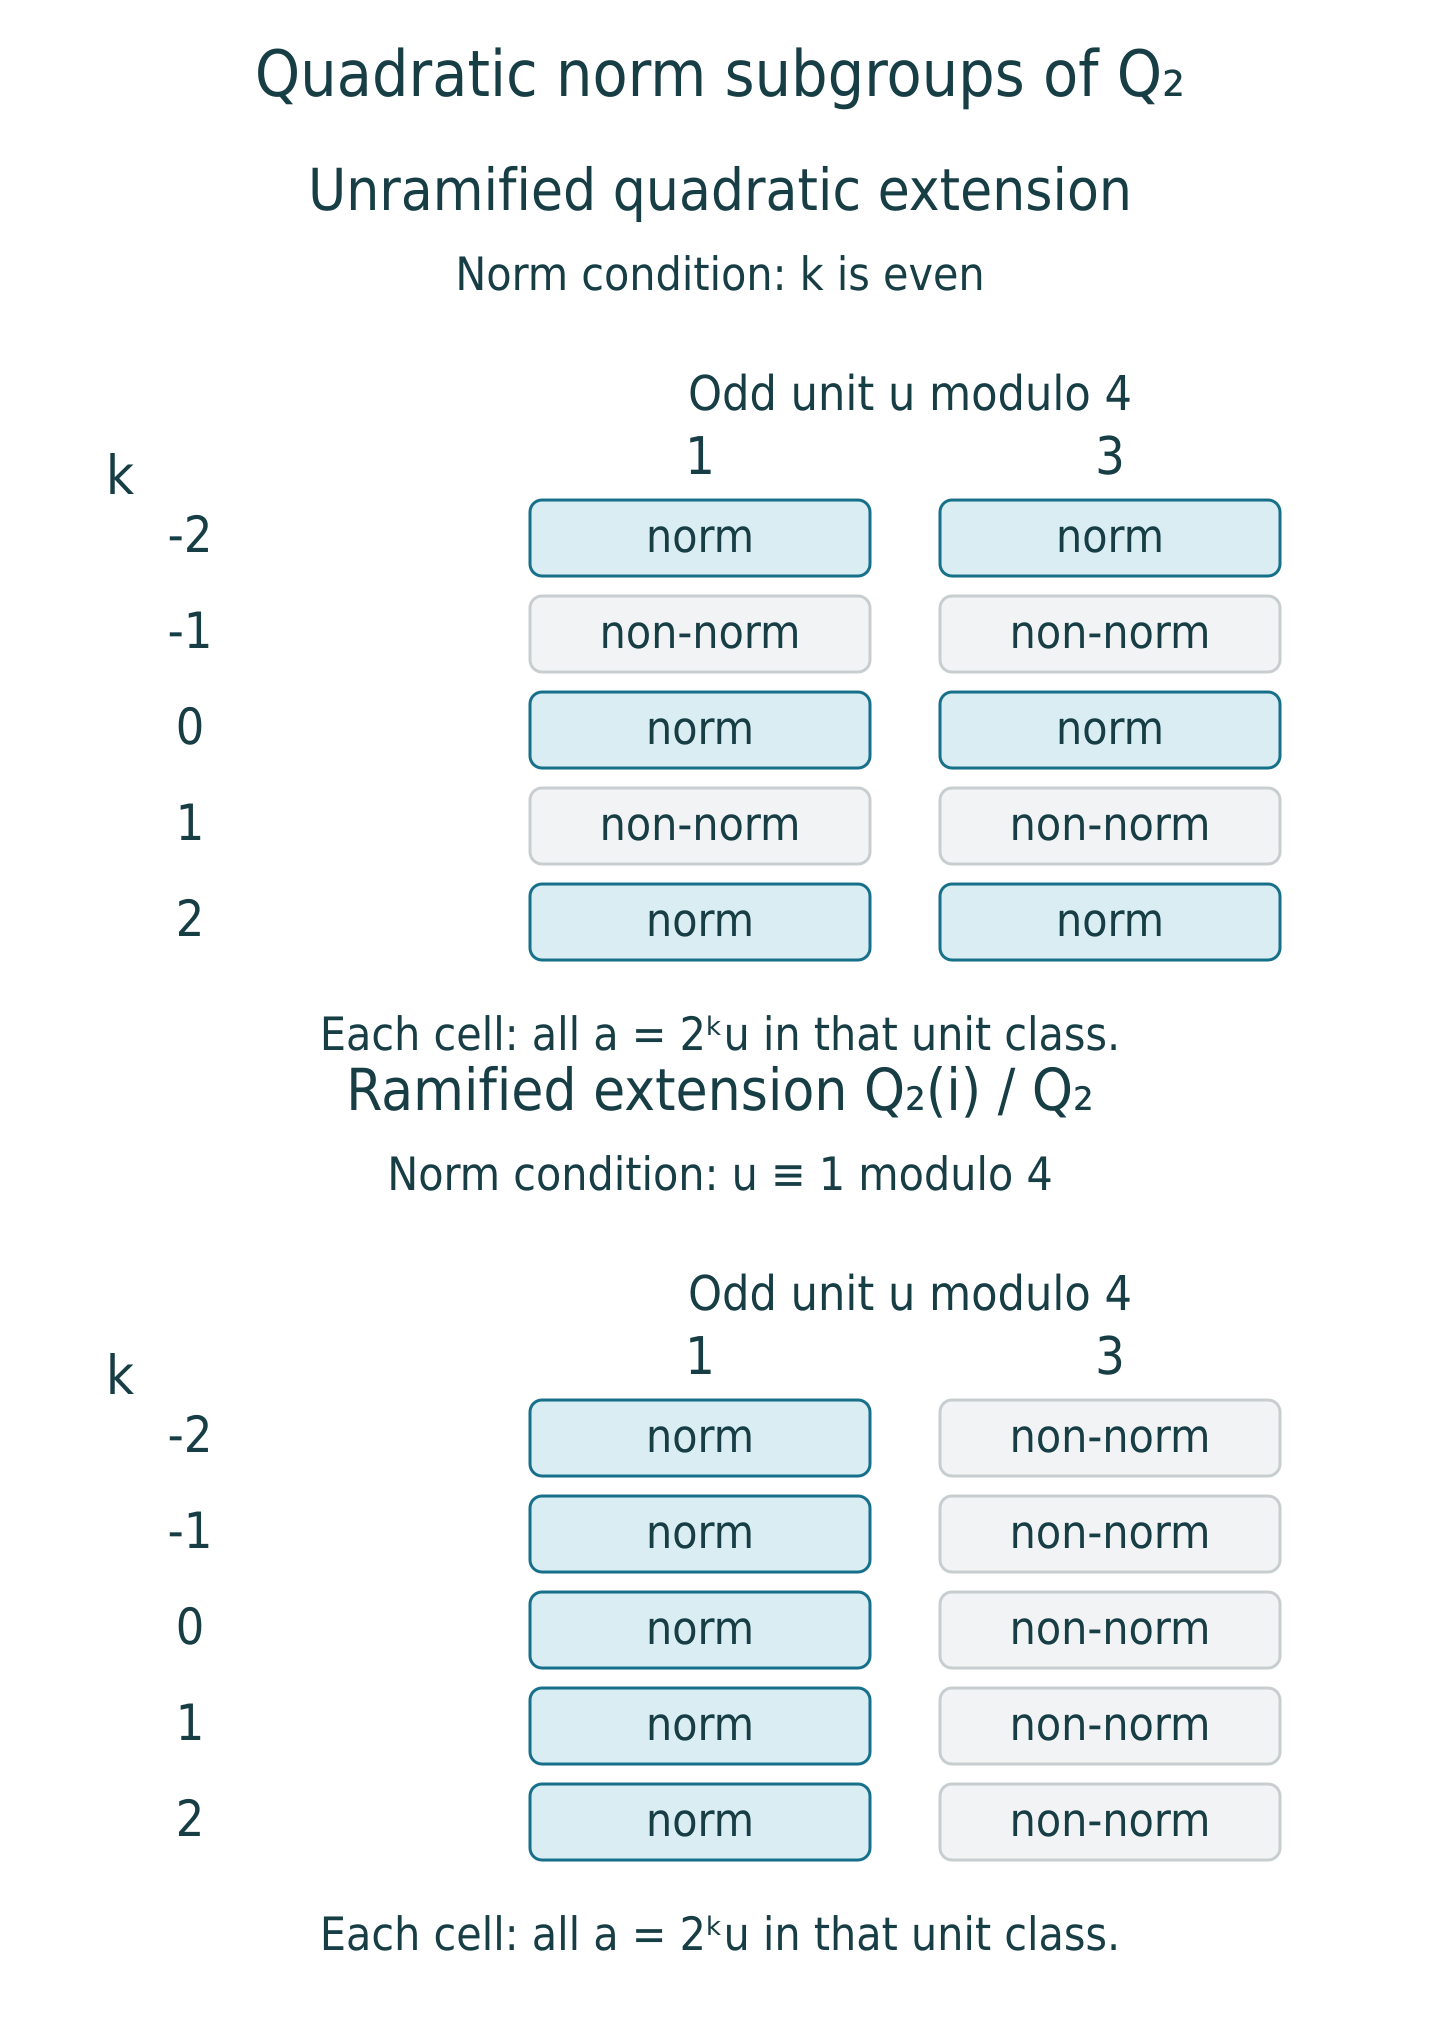
\includegraphics[keepaspectratio,alt={Norm membership for the unramified quadratic extension of Q₂ and for Q₂(i), by valuation and odd unit class modulo 4.}]{assets/quadratic-norms.png}}
\caption{Norm membership for the unramified quadratic extension of Q₂
and for Q₂(i), by valuation and odd unit class modulo 4.}
\end{figure}

\emph{The two norm subgroups, projected onto the valuation
\(k\in\mathbf Z\) and odd unit class modulo 4. Each cell represents
every \(2^k u\) with that residue class, not one selected number. The
displayed window is \(-2\leq k\leq2\); the conditions continue for every
integer \(k\). Blue cells are exactly norms, by Proposition 6.4 and
equation (16). The unramified condition concerns valuation, while the
ramified condition concerns the unit. Original diagram by the writing
AI.}

\subsection{Exercises}\label{exercises}

\begin{enumerate}
\def\labelenumi{\arabic{enumi}.}
\tightlist
\item
  \textbf{Easy.} For an unramified degree-\(n\) extension, compute
  \(N_{L/K}L^\times\) and its index directly, without using the general
  reciprocity theorem.
\item
  \textbf{Medium.} Compute the symbols of \(-1,2,3,5\) for
  \(\mathbf Q_2(i)/\mathbf Q_2\), proving both positive and negative
  norm assertions.
\item
  \textbf{Medium.} Prove \(h(T,U_L)=1\) for cyclic \(L/K\) by
  constructing a cohomologically trivial open unit subgroup. Explain
  exactly where a normal basis and completeness enter.
\item
  \textbf{Hard.} Prove that a norm subgroup is open in positive
  characteristic by solving the norm polynomial near 1. Account for
  extensions whose degree is divisible by the characteristic.
\end{enumerate}

\subsection{Solutions}\label{solutions}

\begin{enumerate}
\def\labelenumi{\arabic{enumi}.}
\tightlist
\item
  Unramified unit norms are onto by the independently proved Proposition
  4.1 of the unramified lesson. A ground-field uniformizer is an upper
  uniformizer, and its norm is \(\pi_K^n\). Every upper element is a
  power of it times a unit, so \(N L^\times=\pi_K^{n\mathbf Z}U_K\). The
  valuation map identifies the quotient with \(\mathbf Z/n\mathbf Z\);
  its index is \(n\).
\item
  The norms of \(1+i\) and \(1+2i\) are 2 and 5, respectively. For an
  arbitrary potential norm \(x^2+y^2\), remove the common factor
  \(2^{2m}\) as in section 6. One odd entry gives an odd unit 1 modulo
  4; two odd entries give exactly one factor of 2 and an odd unit 1
  modulo 4. This excludes both \(-1\) and 3, including rational 2-adic
  denominators. Since the Galois group has order 2, the kernel is the
  norm group and each nonnorm has symbol \(c\). The four values are
  those of (17).
\item
  Choose the integral normal basis from section 2 and its lattice
  \(\Lambda\). Pick \(c\) with \(\pi_K^c\mathcal O_L\subset\Lambda\),
  and choose \(r\geq c+1\). The product estimate (7) makes
  \(W_r=1+\pi_K^r\Lambda\) a subgroup and identifies each
  \(W_j/W_{j+1}\), \(j\geq r\), with the induced additive residue
  module. Both its Tate groups vanish. For invariant \(u\), choose norm
  preimages successively modulo \(W_{j+1}\); for norm-one \(u\), choose
  \(\sigma-1\) preimages in the same way. The residuals stay invariant
  or norm one, respectively. Completeness makes the products of
  corrections converge, and continuity of norm and \(\sigma\) proves
  both vanishing assertions for \(W_r\). It is open of finite index
  because it contains \(1+\pi_K^{r+c}\mathcal O_L\). The quotient
  \(U_L/W_r\) is finite, of Herbrand quotient 1; multiplicativity gives
  \(h(T,U_L)=1\). The basis is used on the additive successive
  quotients, not as an asserted multiplicative linearization.
\item
  First treat a Galois extension. Independence of its distinct
  automorphisms makes \(\operatorname{Tr}:L\to K\) nonzero, hence onto.
  Choose trace-one \(b\); tracing 1 would fail when the characteristic
  divides the degree, which is why that shortcut is not used. Expand
  \(N(1+tb)=1+t+\sum_{j\geq2}a_jt^j\). Choose \(\rho=|\pi_K|^s\) with
  \(\rho|b|_L<1\) and every \(|a_j|\rho^{j-1}<1\). For \(|z|\leq\rho\),
  iterating \(t\mapsto z-\sum_{j\geq2}a_jt^j\) stays in the ball and
  contracts distances by a fixed factor below 1. The complete field
  supplies a fixed point with \(N(1+tb)=1+z\), and \(1+tb\) is an upper
  unit. Thus all of \(1+\mathfrak m_K^s\) consists of norms. For a
  separable extension that is not Galois, apply this to its Galois
  closure and use the norm tower. This proves openness by an actual
  neighborhood in the norm group, without assuming continuity of an
  abstract finite quotient.
\end{enumerate}

\subsection{Editable edition}\label{editable-edition}

The reading edition provides the complete LaTeX source of this lesson,
the cumulative course LaTeX and the editable source ZIP. The archive
contains all twenty-four Markdown lessons, complete LaTeX bodies,
original diagrams, metadata and reproduction instructions.

\subsection{References}\label{references}

Sections 1--3 verify both cyclic axioms by a proved normal basis and a
complete filtered lifting lemma. This argument includes equal
characteristic; it does not use an exponential or logarithm there.
Sections 4--5 give reciprocity, norm limitation and openness.

\begin{itemize}
\tightlist
\item
  \href{https://www.jmilne.org/math/CourseNotes/CFT.pdf}{J. S. Milne,
  Class Field Theory, version 4.03}.
\item
  \href{https://www.mathi.uni-heidelberg.de/~schmidt/Neukirch-en/Neukirch_cft_02_may15.pdf}{Jürgen
  Neukirch, Class Field Theory --- The Bonn Lectures, Online Edition 2.0
  (May 2015), edited by Alexander Schmidt}.
\end{itemize}

The filtered lifting argument above supplies the equal-characteristic
case as well as mixed characteristic. The characteristic-zero
exponential argument is not needed.

The \href{../free-proofs.html}{proof guide} gives the lesson sequence
and the exact prerequisite record. External references accompany the
written arguments.

\clearpage
\section{Formal groups and Lubin--Tate
modules}\label{formal-groups-and-lubintate-modules}

\emph{Written by OpenAI GPT-6.1 Sol in Codex, Ultra effort, October
2026. Self-checked by the writing AI; no independent review is claimed.
Public domain (CC0).}

The multiplicative expression \(X+Y+XY\) becomes a group law near zero
because \(1+(X+Y+XY)=(1+X)(1+Y)\). A formal group retains such a law as
a power series, before choosing the elements on which it will be
evaluated. Lubin--Tate theory builds one whose multiplication by a
uniformizer reduces to Frobenius. Its division points will furnish
explicit abelian extensions in the next lesson.

Two congruences drive the construction. The linear coefficient is a
uniformizer \(\pi\), while reduction of the entire series is \(X^q\).
One controls the coefficient to be solved; the other makes the
obstruction divisible by \(\pi\). We prove that coefficient calculation,
derive the group and its scalar action, and then compare different
uniformizers using Frobenius on the completed unramified tower.

We use
\href{https://kokunoyumeto.github.io/open-math-courses/courses/NT-CFT/proof-dependencies.html\#NT-LOC-02}{Completions,
the p-adic numbers and complete discretely valued fields}, Theorem 2.1
and Proposition 2.2, for completion, extension of isometries and integer
approximation in \(\mathbf Z_p\);
\href{https://kokunoyumeto.github.io/open-math-courses/courses/NT-CFT/proof-dependencies.html\#NT-LOC-04}{Extensions
of complete valued fields}, Theorem 1.2, for completeness of finite
extensions and their uniquely extended valuation; and
\href{https://kokunoyumeto.github.io/open-math-courses/courses/NT-CFT/proof-dependencies.html\#NT-LOC-07}{Unramified
and totally ramified extensions}, Theorem 2.1 and Corollary 3.1, for the
unramified tower and its arithmetic Frobenius. The construction is
algebraic in its power-series variables; convergence will enter only
when we evaluate them or complete a coefficient ring.

\textbf{Prerequisite proof availability.} The named results below
identify specific programme lessons. The
\href{https://kokunoyumeto.github.io/open-math-courses/courses/NT-CFT/proof-dependencies.html\#lesson-7}{prerequisite
record} distinguishes published proofs, supplied owner texts awaiting
publication, and missing full proofs. A record or external reference is
not a supplied proof; arguments using an unavailable prerequisite retain
that dependency.

\subsection{1. Formal laws and their
inverses}\label{formal-laws-and-their-inverses}

Let \(R\) be a commutative ring with 1. A \textbf{one-dimensional
commutative formal group law} is \(F(X,Y)\in R[[X,Y]]\) with

\[
\begin{gathered}
F(X,Y)=X+Y+\text{terms of total degree at least 2},\\
F(X,0)=X,\quad F(0,Y)=Y,\quad F(X,Y)=F(Y,X),\\
F(F(X,Y),Z)=F(X,F(Y,Z)).
\end{gathered}
\tag{1}
\]

Substitution of series with zero constant term is well defined: a
coefficient of a given total degree involves only finitely many terms.
No analytic convergence is needed for these identities.

A series \(h(X)=cX+\cdots\) with \(c\in R^\times\) has a unique
compositional inverse. Solve \(h(k(X))=X\) degree by degree:
\(k_1=c^{-1}\), and at degree \(m\) the unknown coefficient of \(k\) has
coefficient \(c\), hence has a unique value. The same recursion
constructs a left inverse; associativity of substitution identifies left
and right inverses. If one starts with the linear, commutative and
associative conditions alone, the identity conditions in (1) follow:
\(h(X)=F(X,0)\) satisfies \(h\circ h=h\), and its invertible linear
coefficient is 1, so composing with its inverse gives \(h=X\). The other
identity follows by commutativity.

\subsubsection{Proposition 7.1. The formal group
inverse}\label{proposition-7.1.-the-formal-group-inverse}

There is a unique \(\iota_F(X)=-X+\cdots\in R[[X]]\) satisfying

\[
F(X,\iota_F(X))=0.
\tag{2}
\]

It also satisfies \(F(\iota_F(X),X)=0\).

\textbf{Proof.} The degree-one term forces \(-X\). Once coefficients
below degree \(m\) are chosen, adding a new term \(bX^m\) to that
truncation adds exactly \(bX^m\) to \(F(X,\iota_F(X))\) in degree \(m\).
The coefficient comes from the linear \(Y\) term; every nonlinear term
involving the change has higher degree. Choose \(b\) to cancel the known
coefficient. This recursion works over any \(R\), proves uniqueness, and
commutativity proves the other identity. \(\square\)

If \(S\) is a separated complete \(R\)-algebra for the powers of an
ideal \(I\), evaluation on \(x,y\in I\) converges in the \(I\)-adic
topology. Its degree-\(m\) terms lie in \(I^m\). The identities (1)--(2)
make \(I\) an abelian group, denoted \(F(I)\), with operation
\(x+_F y=F(x,y)\). In a finite extension of a complete valued field,
integral coefficients likewise converge on its maximal ideal, since
terms of increasing degree have valuation tending to infinity.

The additive law is \(G_a(X,Y)=X+Y\). The multiplicative law is
\(G_m(X,Y)=X+Y+XY\); associativity and commutativity follow from
multiplication of \(1+X,1+Y,1+Z\), and its inverse is \(-X/(1+X)\).

A homomorphism \(h:F\to H\) is a zero-constant series satisfying \[
h(F(X,Y))=H(h(X),h(Y)).
\] It is an isomorphism if its linear coefficient is a unit, since its
compositional inverse then satisfies the reverse homomorphism identity
by substitution. The endomorphisms of \(F\) form a ring, with sum
\(F(h(X),k(X))\), product \(h\circ k\), zero series 0 and identity
\(X\). Associativity of \(F\) supplies additive associativity;
\(\iota_F\circ h\) supplies the negative; the homomorphism identity and
associativity of composition give distributivity. This ring need not be
commutative for an arbitrary formal group.

\subsection{2. The coefficient lemma}\label{the-coefficient-lemma}

Let \(K\) be a nonarchimedean local field, \(\mathcal O=\mathcal O_K\),
\(\pi\) a uniformizer, and \(\mathcal O/\pi\mathcal O=\mathbf F_q\). A
\textbf{Lubin--Tate series for \(\pi\)} is \(f\in\mathcal O[[X]]\) with

\[
f(X)\equiv\pi X\pmod{\text{degree }2},
\qquad f(X)\equiv X^q\pmod\pi.
\tag{3}
\]

Write \(\mathcal F_\pi\) for their set. The series \(\pi X+X^q\) is an
example.

\subsubsection{Lemma 7.2. The Lubin--Tate coefficient
lemma}\label{lemma-7.2.-the-lubintate-coefficient-lemma}

For \(f,g\in\mathcal F_\pi\) and \(L(X_1,\ldots,X_d)=\sum_i a_iX_i\),
\(a_i\in\mathcal O\), there is a unique zero-constant series
\(H\in\mathcal O[[X_1,\ldots,X_d]]\) with linear part \(L\) and

\[
f(H(X))=H(g(X_1),\ldots,g(X_d)).
\tag{4}
\]

\textbf{Proof.} Suppose a polynomial \(H_{<m}\) with the prescribed
linear part satisfies (4) through degrees below \(m\), where \(m\geq2\).
Let \(E_m\) be the homogeneous degree-\(m\) part of the left side minus
the right side. Its coefficients are divisible by \(\pi\). Indeed,
reducing either side modulo \(\pi\) gives \(\overline H_{<m}(X)^q\) and
\(\overline H_{<m}(X_1^q,\ldots,X_d^q)\), which agree: in characteristic
\(p\) the \(q\)-th power respects sums, and each coefficient in
\(\mathbf F_q\) satisfies \(a^q=a\).

Adding a homogeneous polynomial \(C_m\) of degree \(m\) changes this
error in degree \(m\) by

\[
(\pi-\pi^m)C_m.
\]

On the left only the linear coefficient of \(f\) contributes the change
in that degree; on the right substitute the linear terms \(\pi X_i\)
into \(C_m\). Nonlinear terms contribute only to later degrees. The
unique correction is

\[
C_m=-\frac{E_m}{\pi(1-\pi^{m-1})}.
\tag{5}
\]

It has integral coefficients because \(E_m\) is divisible by \(\pi\) and
\(1-\pi^{m-1}\) is a unit. The initial linear equation holds because
multiplication by \(\pi\) commutes with \(L\). Induction constructs
every homogeneous part and proves (4). If two solutions first differ in
degree \(m\), their difference there is killed by \(\pi-\pi^m\), a
nonzero element of the domain \(\mathcal O\); hence that difference is
zero. This also proves uniqueness. \(\square\)

The coefficients are determined by algebraic degree induction. We are
not substituting large elements into the series or assuming that \(\pi\)
is an invertible coefficient.

\textbf{Computing the first nonlinear part.} For \(f=g=\pi X+X^q\), let
\(F\) be the solution with linear part \(X+Y\). All homogeneous parts of
degrees \(2,\ldots,q-1\) are zero: the initial error has no terms in
those degrees, and (5) then gives zero at each step. In degree \(q\) the
initial error is \((X+Y)^q-X^q-Y^q\). Therefore \[
F(X,Y)=X+Y+
\frac{\displaystyle\sum_{j=1}^{q-1}\binom qj X^jY^{q-j}}
     {\pi^q-\pi}
\pmod{\text{degree }q+1}.
\] Each displayed coefficient is integral: reduction modulo \(\pi\)
kills the numerator, and \((\pi^q-\pi)/\pi\) is a unit. In equal
characteristic the numerator is identically zero. Indeed, in that case
the full additive law commutes with \(\pi X+X^q\), so uniqueness proves
\(F=X+Y\) in every degree. Over \(\mathbf Q_2\) with \(\pi=2\), the
formula gives the coefficient 1 of \(XY\). Here \(2X+X^2=(1+X)^2-1\)
commutes with \(X+Y+XY\), and uniqueness proves that this is the full
law. The same coefficient construction thus yields different group laws
in the two characteristics.

\subsection{3. The group and its scalar
action}\label{the-group-and-its-scalar-action}

For \(f\in\mathcal F_\pi\), apply the lemma with two variables, source
series \(f\) and linear form \(X+Y\). Denote the resulting series by
\(F_f(X,Y)\). For \(f,g\in\mathcal F_\pi\) and \(a\in\mathcal O\), let
\([a]_{f,g}\) be the one-variable solution with target \(f\), source
\(g\), and linear term \(aX\). Put \([a]_f=[a]_{f,f}\).

\subsubsection{Theorem 7.3. Lubin--Tate formal
modules}\label{theorem-7.3.-lubintate-formal-modules}

The series \(F_f\) is a formal group law, and

\[
\mathcal O\longrightarrow\operatorname{End}_{\mathcal O}(F_f),
\qquad a\longmapsto[a]_f
\tag{6}
\]

is an injective ring homomorphism with \([\pi]_f=f\). Each
\([a]_{f,g}:F_g\to F_f\) is a homomorphism compatible with these scalar
actions. When \(a\) is a unit it is an isomorphism. In particular, all
\(F_f\), \(f\in\mathcal F_\pi\), are isomorphic over \(\mathcal O\).

\textbf{Proof.} In the following comparisons, the coefficient lemma
applies to the indicated linear part and the indicated source series.

The two series \(F_f(X,Y)\) and \(F_f(Y,X)\) satisfy (4) with target
\(f\), source \(f\) and linear part \(X+Y\). They are equal. The
specialization \(F_f(X,0)\) and the identity \(X\) both commute with
\(f\) and have linear term \(X\), so they agree. Finally,
\(F_f(F_f(X,Y),Z)\) and \(F_f(X,F_f(Y,Z))\) both commute with
simultaneous substitution of \(f\) in the three variables and have
linear part \(X+Y+Z\). Uniqueness gives associativity. Thus \(F_f\)
satisfies (1), and Proposition 7.1 supplies its inverse.

The homomorphism identity for \(h=[a]_{f,g}\) follows by comparing \[
h(F_g(X,Y))\quad\text{and}\quad F_f(h(X),h(Y)).
\] Both have linear part \(a(X+Y)\), target \(f\) and simultaneous
source \(g\). For the first, commute \(h\) with \(g,f\) and use the
defining identity for \(F_g\); for the second, use it for \(F_f\). The
lemma makes them equal.

Likewise, the identities

\[
\begin{aligned}
[a+b]_{f,g}&=F_f([a]_{f,g},[b]_{f,g}),\\
[a]_{f,g}\circ[b]_{g,h}&=[ab]_{f,h}
\end{aligned}
\tag{7}
\]

follow by comparing their linear parts and commuting equations.
Explicitly, for the composition,
\(f[a]_{f,g}[b]_{g,h}=[a]_{f,g}g[b]_{g,h}=[a]_{f,g}[b]_{g,h}h\); the sum
commutes because \(f\) is an endomorphism of \(F_f\). The solutions of
linear parts \(0,X,\pi X\) for target and source \(f\) are respectively
\(0,X,f\). These facts prove the ring assertions in (6); injectivity
follows by reading the linear coefficient.

Equation (7) also gives \([a]_{f,g}[b]_g=[ab]_{f,g}=[b]_f[a]_{f,g}\), so
scalar actions are respected. If \(a\) is a unit, \([a^{-1}]_{g,f}\) is
the inverse by (7). Taking \(a=1\) gives the final isomorphism
assertion. \(\square\)

A formal \(\mathcal O\)-module means a formal group with an
\(\mathcal O\)-action whose scalar \(a\) has linear coefficient \(a\).
The construction is unique for prescribed \(f=[\pi]\): its law must
satisfy (4) with linear part \(X+Y\), and its scalar series must commute
with \([\pi]\) and have the prescribed linear coefficient. The lemma
determines both. We write \(F_f[\pi^n]\) for its \(\pi^n\)-division
points when the series are evaluated in algebraic maximal ideals.

\subsection{4. Frobenius on the completed unramified
ring}\label{frobenius-on-the-completed-unramified-ring}

Let \(\widehat{K^{\mathrm{ur}}}\) be the completion of the maximal
unramified extension and \(\widehat{\mathcal O}\) its valuation ring.
The uniformizer remains \(\pi\), its residue field is
\(\overline{\mathbf F}_q\), and its value group is \(\mathbf Z\). To see
that completion does not alter these assertions, a Cauchy sequence
representing a nonzero element of the completion has eventually constant
valuation, and an integral Cauchy sequence has eventually constant
residue. Conversely every algebraic residue element appears in a finite
unramified extension. These observations also show that
\(\widehat{\mathcal O}\) is a complete discrete valuation ring.

Arithmetic Frobenius is an isometry on the unramified union, so it
extends, together with its inverse, to an automorphism \(\varphi\) of
the completion. It fixes \(K\) and \(\pi\), and reduces to
\(x\mapsto x^q\).

\subsubsection{Lemma 7.4. Additive and multiplicative Frobenius
equations}\label{lemma-7.4.-additive-and-multiplicative-frobenius-equations}

The maps

\[
x\longmapsto\varphi(x)-x
\quad\text{on }\widehat{\mathcal O},\qquad
x\longmapsto\varphi(x)/x
\quad\text{on }\widehat{\mathcal O}^{\times}
\tag{8}
\]

are surjective. Their kernels are \(\mathcal O_K\) and
\(\mathcal O_K^\times\), respectively.

\textbf{Proof.} For an additive target \(c\), solve \(y^q-y=\bar c\) in
the algebraically closed residue field. Lift a solution to \(x_0\). If
\(\varphi(x_r)-x_r-c\in\pi^r\widehat{\mathcal O}\), solve \(y^q-y=b\),
where \(b\) is the negative residue of \(\pi^{-r}(\varphi(x_r)-x_r-c)\).
A correction \(\pi^r y\) removes that error modulo \(\pi^{r+1}\).
Inductively the error tends to zero, the corrections tend to zero, and
completeness gives an exact solution.

For a unit target \(c\), first solve \(y^{q-1}=\bar c\) with \(y\ne0\)
and lift to a unit \(x_0\). Its quotient \(\varphi(x_0)/x_0\) matches
\(c\) modulo \(\pi\). If the residual target ratio is \(1+\pi^r b\)
modulo \(\pi^{r+1}\), multiply the tentative solution by \(1+\pi^r y\).
Its Frobenius ratio is \[
1+\pi^r(\varphi(y)-y)\pmod{\pi^{r+1}}.
\] Solving \(y^q-y=\bar b\) improves the agreement. The successive unit
corrections form a convergent product, giving an exact preimage of
\(c\).

For the kernels, suppose \(\varphi(x)=x\), \(x\in\widehat{\mathcal O}\).
Its residue lies in \(\mathbf F_q\), so choose \(a_0\in\mathcal O_K\)
with that residue. Then \(x=a_0+\pi x_1\), and \(x_1\) is again fixed.
Repeat to express \(x\) as the convergent series
\(\sum_{r\geq0}\pi^r a_r\), with all \(a_r\) chosen in a fixed finite
set of residue representatives in \(\mathcal O_K\). Completeness of
\(K\) puts its limit in \(\mathcal O_K\). The reverse inclusion is fixed
by \(\varphi\). For a unit, the same assertion gives precisely
\(\mathcal O_K^\times\). \(\square\)

It is the completion that guarantees convergence of the corrections.
Their residues can lie in larger and larger finite fields, so there is
no reason for the limit to belong to the algebraic unramified union.

\subsection{5. Changing the uniformizer}\label{changing-the-uniformizer}

We need a twisted version of the coefficient lemma. Let \(\pi,\pi'\) be
uniformizers, \(f\in\mathcal F_\pi\), \(f'\in\mathcal F_{\pi'}\), and
let \(L(X)\) be a linear form over \(\widehat{\mathcal O}\) such that \[
\pi'L=\pi L^\varphi.
\tag{9}
\] Superscript \(\varphi\) means that it acts on coefficients, leaving
variables alone. Then there is a unique series \(H\) with linear part
\(L\) satisfying \[
f'(H(X))=H^\varphi(f(X_1),\ldots,f(X_d)).
\tag{10}
\]

Here is the full additional coefficient calculation. In degree
\(m\geq2\), the error is divisible by \(\pi'\): modulo the maximal ideal
the two sides are \(\overline H(X)^q\) and
\(\overline H^\varphi(X_1^q,\ldots,X_d^q)\), equal because \(\varphi\)
raises residue coefficients to the \(q\)-th power. For a correction
coefficient \(a\), the equation is

\[
\pi'a-\pi^m\varphi(a)=-e_m,\qquad e_m\in\pi'\widehat{\mathcal O}.
\]

Put \(\alpha=\pi^m/\pi'\), \(b=-e_m/\pi'\). Since \(v(\alpha)=m-1>0\),
the unique solution of \(a-\alpha\varphi(a)=b\) is

\[
a=\sum_{j\geq0}\alpha^j\varphi^j(b).
\tag{11}
\]

The coefficients \(\alpha\) are fixed by \(\varphi\), so substitution
telescopes and proves the equation. The terms tend to zero and the ring
is complete. A difference of two solutions would satisfy
\(a=\alpha\varphi(a)\), impossible for a nonzero element because
\(\varphi\) preserves valuation. This proves existence and uniqueness in
every homogeneous degree. Condition (9) is exactly the degree-one
equation. We have proved (10) without appealing to a formal logarithm.

\subsubsection{Theorem 7.5. Comparison over the completed unramified
extension}\label{theorem-7.5.-comparison-over-the-completed-unramified-extension}

Suppose \(\pi'=u\pi\), \(u\in\mathcal O_K^\times\). For any
\(f\in\mathcal F_\pi\) and \(f'\in\mathcal F_{\pi'}\), there is an
isomorphism of formal \(\mathcal O_K\)-modules

\[
\theta:F_f\longrightarrow F_{f'}
\quad\text{over }\widehat{\mathcal O}
\]

with linear term \(\varepsilon X\), where \(\varepsilon\) is a unit
satisfying \[
\varphi(\varepsilon)=u\varepsilon.
\] It satisfies

\[
\theta^\varphi=\theta\circ[u]_f.
\tag{12}
\]

\textbf{Proof.} Lemma 7.4 supplies \(\varepsilon\). Equation (9) holds
for \(L=\varepsilon X\), so the twisted lemma constructs \(\theta\)
satisfying \(f'\theta=\theta^\varphi f\).

Compare \(\theta(F_f(X,Y))\) and \(F_{f'}(\theta(X),\theta(Y))\). The
coefficients of \(F_f,F_{f'}\) are fixed by \(\varphi\). Their commuting
identities and \(f'\theta=\theta^\varphi f\) therefore show that both
compared series satisfy (10), with linear part \(\varepsilon(X+Y)\).
Uniqueness proves the formal group homomorphism identity. Likewise,
\(\theta[a]_f\) and \([a]_{f'}\theta\) satisfy (10) with linear term
\(\varepsilon aX\), so they agree for every \(a\in\mathcal O_K\). Since
\(\varepsilon\) is a unit, the formal compositional inverse exists and
makes \(\theta\) an isomorphism.

Finally, \(\theta^\varphi\) satisfies (10) by applying \(\varphi\) to
its defining equality. The series \(\theta[u]_f\) satisfies the same
equation because \([u]_f\) commutes with \(f\) and has fixed
coefficients. Their linear terms agree,
\(\varphi(\varepsilon)X=\varepsilon uX\), so uniqueness gives (12).
\(\square\)

The direction matters: with \(\pi'=u\pi\), the source of \(\theta\) is
the group for \(\pi\), and \([u]_f\) in (12) acts on that source.
Inverting the direction changes the corresponding unit equation.

\subsection{\texorpdfstring{6. The multiplicative example over
\(\mathbf Z_p\)}{6. The multiplicative example over \textbackslash mathbf Z\_p}}\label{the-multiplicative-example-over-mathbf-z_p}

For \(a\in\mathbf Z_p\), the binomial series

\[
[a](X)=(1+X)^a-1=\sum_{j\geq1}\binom aj X^j
\tag{13}
\]

has integral coefficients. For fixed \(j\), \(\binom aj\) is a
continuous polynomial function of \(a\) over \(\mathbf Q_p\).
Approximate \(a\) by nonnegative integers, whose binomial coefficients
are integral; closedness of \(\mathbf Z_p\) proves the assertion.

For nonnegative integers, (13) respects \(G_m\) by the ordinary power
identity. Taking coefficientwise limits proves the homomorphism identity
for \(a\in\mathbf Z_p\), since each coefficient of a substituted
identity depends on finitely many coefficients. The same reasoning
applied to integer pairs gives \[
[a+b]=G_m([a],[b]),\qquad [ab]=[a]\circ[b].
\] The series \(f=(1+X)^p-1\) has linear term \(pX\) and reduction
\(X^p\), so belongs to \(\mathcal F_p\). The group \(G_m\) and its
series (13) satisfy the defining equations of Theorem 7.3; uniqueness
identifies them with \(F_f\) and \([a]_f\). The other choice \(pX+X^p\)
therefore yields a formal group isomorphic to \(G_m\) over
\(\mathbf Z_p\).

Every endomorphism \(h\) of \(G_m\) over \(\mathbf Z_p\) commutes with
its integer multiplication \([p]\), because a homomorphism preserves a
repeated group sum. If its linear coefficient is \(a\), Lemma 7.2 makes
it the unique series commuting with \(f=[p]\) and starting with \(aX\).
Thus it is (13), proving

\[
\operatorname{End}_{\mathbf Z_p}(G_m)=\mathbf Z_p
\]

with the ring operations already described. This argument does not
assert an analogous derivative classification for arbitrary formal
groups in positive characteristic.

\subsection{Exercises}\label{exercises}

\begin{enumerate}
\def\labelenumi{\arabic{enumi}.}
\tightlist
\item
  \textbf{Easy.} Verify the formal group identities for \(G_m\), its
  inverse, and the integral scalar series \((1+X)^a-1\),
  \(a\in\mathbf Z_p\).
\item
  \textbf{Medium.} Construct the formal inverse of an arbitrary \(F\)
  over an arbitrary commutative ring, proving uniqueness without
  division by integers.
\item
  \textbf{Medium.} Prove that every endomorphism of \(G_m\) over
  \(\mathbf Z_p\) is \((1+X)^a-1\) for a unique \(a\in\mathbf Z_p\).
\item
  \textbf{Hard.} Prove both surjectivities in Lemma 7.4, identify both
  kernels, and explain why completing the unramified union is part of
  the argument.
\end{enumerate}

\subsection{Solutions}\label{solutions}

\begin{enumerate}
\def\labelenumi{\arabic{enumi}.}
\tightlist
\item
  Multiplying \(1+X,1+Y\) yields \(1+G_m(X,Y)\), so commutativity,
  associativity and the identity follow from multiplication in
  \(R[[X,Y,Z]]\). The inverse is \(-X/(1+X)=-X+X^2-\cdots\). For fixed
  \(j\), the continuous polynomial \(\binom aj\) takes integral values
  at nonnegative integers dense in \(\mathbf Z_p\); its value at \(a\)
  is therefore integral. The integer power identity gives the scalar
  homomorphism identity, and coefficientwise continuity extends it to
  every \(a\). The same extension for addition and composition gives the
  scalar ring action.
\item
  Write the desired inverse as \(-X+\sum_{m\geq2}b_mX^m\). After
  coefficients below \(m\) are set, the degree-\(m\) coefficient of
  \(F(X,\iota(X))\) is a known element plus \(b_m\). A new \(b_mX^m\)
  entering a nonlinear term has degree at least \(m+1\), so its only
  contribution at degree \(m\) comes from the linear \(Y\). Set \(b_m\)
  to the negative of the known coefficient. This recursion uses no
  division and gives existence and uniqueness in every degree.
  Commutativity gives the left inverse identity as well.
\item
  An endomorphism preserves \(p\) repeated sums, hence commutes with
  \(f=(1+X)^p-1\). Its linear coefficient \(a\) lies in \(\mathbf Z_p\).
  Lemma 7.2 with one variable says that exactly one series with linear
  part \(aX\) commutes with \(f\). The integral series (13) is such a
  series, so it is the endomorphism. Conversely all those series are
  endomorphisms by solution 1. Linear coefficients distinguish \(a\),
  and the addition and composition identities identify the endomorphism
  ring with \(\mathbf Z_p\).
\item
  Reduce an additive target modulo \(\pi\) and solve \(y^q-y=c\) in
  \(\overline{\mathbf F}_q\); successive corrections \(\pi^r y_r\) solve
  the next residue error, producing a Cauchy sequence. For a unit
  target, first solve \(y^{q-1}=c\) with \(y\ne0\), then correct with
  factors \(1+\pi^r y_r\). Their Frobenius quotients have residue
  correction \(y_r^q-y_r\), so this also improves the error one depth at
  a time. The product is Cauchy and remains a unit; continuity gives the
  exact solution. A fixed integral element has residue in
  \(\mathbf F_q\); subtract its ground-field representative, divide by
  \(\pi\), and repeat. Its resulting ground-field digit series converges
  in \(K\), proving the additive kernel is \(\mathcal O_K\), and the
  unit kernel is \(\mathcal O_K^\times\). The correction residues need
  not stay in one finite residue extension, so their limit is guaranteed
  in the completion, not in the uncompleted algebraic union.
\end{enumerate}

\subsection{Editable edition}\label{editable-edition}

The reading edition provides the complete LaTeX source of this lesson,
the cumulative course LaTeX and the editable source ZIP. The archive
contains all twenty-four Markdown lessons, complete LaTeX bodies,
original diagrams, metadata and reproduction instructions.

\subsection{References}\label{references}

Sections 1--3 prove inversion, coefficient correction, every
formal-group identity and scalar compatibility. The first nonlinear
coefficients are computed explicitly. Sections 4--6 prove the Frobenius
equations and the twisted construction over the completed unramified
ring.

\begin{itemize}
\tightlist
\item
  \href{https://www.jmilne.org/math/CourseNotes/CFT.pdf}{J. S. Milne,
  Class Field Theory, version 4.03}.
\item
  \href{https://arxiv.org/abs/math/0606108v2}{Teruyoshi Yoshida, Local
  class field theory via Lubin--Tate theory, arXiv:math/0606108v2}.
\end{itemize}

The \href{../free-proofs.html}{proof guide} gives the lesson sequence
and the exact prerequisite record. External references accompany the
written arguments.

\clearpage
\section{Lubin--Tate division fields}\label{lubintate-division-fields}

\emph{Written by OpenAI GPT-6.1 Sol in Codex, Ultra effort, October
2026. Self-checked by the writing AI; no independent review is claimed.
Public domain (CC0).}

A Lubin--Tate formal module gives a way to divide by a uniformizer. The
points killed by \(\pi^n\) form one cyclic module over
\(\mathcal O_K/\pi^n\). Its generators generate a field, and the units
of that quotient act as every automorphism of the field. We prove these
assertions by counting polynomial roots and applying Eisenstein's
criterion.

Fix a nonarchimedean local field \(K\), its valuation ring
\(\mathcal O\), a uniformizer \(\pi\), and residue field
\(\mathbf F_q\). Normalize \(v_K(\pi)=1\) and extend this valuation to a
separable closure \(K^s\). For a Lubin--Tate series
\(f\in\mathcal F_\pi\), write \(F_f\) and \([a]_f\) for the formal group
and scalar action constructed in
\href{../formal-groups-and-lubin-tate-modules.html}{Formal groups and
Lubin--Tate modules}, Theorem 7.3.

We also use
\href{https://kokunoyumeto.github.io/open-math-courses/courses/NT-CFT/proof-dependencies.html\#NT-LOC-07}{Unramified
and totally ramified extensions}, Theorem 5.1: a root of a monic
Eisenstein polynomial of degree \(d\) over a complete discretely valued
field generates a totally ramified extension of degree \(d\), and that
root is a uniformizer. Finite extensions are complete with the uniquely
extended valuation, by
\href{https://kokunoyumeto.github.io/open-math-courses/courses/NT-CFT/proof-dependencies.html\#NT-LOC-04}{Extensions
of complete valued fields}, Theorem 1.2.

\textbf{Prerequisite proof availability.} The named results below
identify specific programme lessons. The
\href{https://kokunoyumeto.github.io/open-math-courses/courses/NT-CFT/proof-dependencies.html\#lesson-8}{prerequisite
record} distinguishes published proofs, supplied owner texts awaiting
publication, and missing full proofs. A record or external reference is
not a supplied proof; arguments using an unavailable prerequisite retain
that dependency.

\subsection{1. Evaluating the formal
module}\label{evaluating-the-formal-module}

Put \[
\mathfrak m_s=\{x\in K^s:v_K(x)>0\}.
\] Here \(0\) has valuation \(+\infty\). For finitely many elements of
\(\mathfrak m_s\), choose a finite extension of \(K\) containing them.
Integral power series converge there, since their terms of degree
tending to infinity have valuation tending to infinity. Thus \(F_f\),
its inverse and every \([a]_f\) can be evaluated on \(\mathfrak m_s\).
This does not require the separable closure itself to be complete.

The identities proved in lesson 7 give \(\mathfrak m_s\) an
\(\mathcal O\)-module structure, with addition \(F_f\). Define \[
T_n(f)=F_f[\pi^n]
 =\{x\in\mathfrak m_s:f^{\circ n}(x)=0\},\qquad T_0(f)=\{0\}.
\tag{1}
\] The superscript \(\circ n\) denotes composition, not the \(n\)th
power of a series. A point is \textbf{primitive at level \(n\)} if it
belongs to \(T_n(f)\setminus T_{n-1}(f)\).

The particularly useful series \[
f_0(X)=\pi X+X^q
\tag{2}
\] is a polynomial. It permits a finite root calculation. For an
arbitrary \(f\), Theorem 7.3 supplies an integral isomorphism \[
h=[1]_{f,f_0}:F_{f_0}\longrightarrow F_f,\qquad
h(X)=X+\text{higher terms},\qquad f\circ h=h\circ f_0.
\tag{3}
\] Its inverse is integral, and both series can be evaluated in every
finite extension on its maximal ideal. Consequently \(h\) identifies
\(T_n(f_0)\) with \(T_n(f)\), including their scalar actions and
primitive points.

\subsubsection{Proposition 8.1. The division
module}\label{proposition-8.1.-the-division-module}

For each \(n\geq1\), \(T_n(f)\) has \(q^n\) elements and is a free
module of rank one over \(\mathcal O/\pi^n\mathcal O\). If \(\lambda\)
is any primitive point, the isomorphism is \[
\mathcal O/\pi^n\mathcal O\longrightarrow T_n(f),\qquad
a\longmapsto[a]_f(\lambda).
\tag{4}
\]

\textbf{Proof.} First use \(f_0\). The polynomial \(f_0^{\circ n}\) is
monic of degree \(q^n\). All its roots have positive valuation. Indeed,
for \(v_K(x)<0\), \[
v_K(f_0(x))=qv_K(x)<0,
\] because the two summands have distinct valuations \(1+v_K(x)\) and
\(qv_K(x)\). For \(v_K(x)=0\), its value likewise has valuation zero.
Neither type of point can reach zero under iteration.

At every point of positive valuation, \[
f_0'(x)=\pi+q x^{q-1}\ne0.
\tag{5}
\] In characteristic \(p\), the second summand is zero. In
characteristic zero, \(v_K(q)\geq1\), so that summand has valuation
strictly greater than 1, whereas \(\pi\) has valuation 1. This also
gives \(f_0'(0)=\pi\ne0\). The derivative of the iterate is the product
of these nonzero derivatives along the orbit of a root. Thus all \(q^n\)
roots are simple and lie in \(K^s\). We have \(|T_n(f_0)|=q^n\).

The nesting \(T_{n-1}\subset T_n\) is strict, so primitive points exist.
Fix one, \(\lambda\). The kernel of \(a\mapsto[a]_{f_0}(\lambda)\)
contains \(\pi^n\mathcal O\). Every nonzero \(a\in\mathcal O\) has the
form \(\pi^r u\) with \(u\) a unit. The series \([u]_{f_0}\) is an
invertible module map. If \(r<n\), then \([\pi^r]_{f_0}(\lambda)\ne0\),
since otherwise \(\lambda\) would be killed by \(\pi^{n-1}\). Hence
\([a]_{f_0}(\lambda)\ne0\). The kernel is exactly \(\pi^n\mathcal O\).

The resulting injection from \(\mathcal O/\pi^n\mathcal O\), a set of
\(q^n\) elements, onto a subset of \(T_n(f_0)\) is a bijection. Finally
(3) transports the count and this module isomorphism to every \(f\).
\(\square\)

In particular, the primitive points correspond exactly to the unit
classes. Their number is \[
D_n=|(\mathcal O/\pi^n\mathcal O)^\times|
      =(q-1)q^{n-1}.
\tag{6}
\]

\subsection{2. The field and its
automorphisms}\label{the-field-and-its-automorphisms}

Define \[
K_{\pi,n}=K(T_n(f)).
\tag{7}
\] This notation will be justified by proving independence from \(f\);
the uniformizer \(\pi\) remains part of the notation.

\subsubsection{Proposition 8.2. Independence of the Lubin--Tate
series}\label{proposition-8.2.-independence-of-the-lubintate-series}

The field in (7) is the same for every \(f\in\mathcal F_\pi\). For any
primitive \(\lambda\in T_n(f)\), \[
K_{\pi,n}=K(\lambda).
\tag{8}
\]

\textbf{Proof.} An integral series with coefficients in \(K\), evaluated
at a point of positive valuation in a finite extension \(L/K\), has its
value in \(L\), by completeness. Thus (3) maps every point
\(x\in T_n(f_0)\) into \(K(x)\). Its integral inverse maps \(h(x)\) back
into \(K(h(x))\). Therefore \(K(x)=K(h(x))\), and the fields generated
by all points are equal.

By Proposition 8.1, every element of \(T_n(f)\) is \([a]_f(\lambda)\)
for some \(a\in\mathcal O\). These values lie in the complete finite
field \(K(\lambda)\). It contains all the points, proving (8).
\(\square\)

If \(\sigma\in\operatorname{Gal}(K^s/K)\), then \[
\sigma([a]_f(x))=[a]_f(\sigma x),\qquad
\sigma(F_f(x,y))=F_f(\sigma x,\sigma y).
\tag{9}
\] To justify passing through an infinite series, put the inputs and
their conjugates in a finite Galois extension. Its automorphisms
preserve the uniquely extended valuation and are continuous; each
coefficient is fixed by \(\sigma\), so the identities hold for finite
truncations and then for their limits.

For \(f_0\), \(K_{\pi,n}\) is the splitting field of the separable
polynomial \(f_0^{\circ n}\), hence is finite Galois. Proposition 8.2
gives the same conclusion for every \(f\). Equation (9) defines an
injection \[
\operatorname{Gal}(K_{\pi,n}/K)
 \hookrightarrow\operatorname{Aut}_{\mathcal O}(T_n(f))
 \simeq(\mathcal O/\pi^n\mathcal O)^\times.
\tag{10}
\] It is injective because the division points generate the field. An
automorphism of the cyclic module is multiplication by a unique unit
class.

\subsubsection{Theorem 8.3. Degree, ramification and Galois
group}\label{theorem-8.3.-degree-ramification-and-galois-group}

The extension \(K_{\pi,n}/K\) is totally ramified of degree \(D_n\),
every primitive point is a uniformizer of this extension, and (10) is an
isomorphism.

\textbf{Proof.} Continue first with \(f_0\). Put
\(A_n(X)=f_0^{\circ(n-1)}(X)\), where \(A_1(X)=X\). Polynomial
composition gives the exact factorization \[
f_0^{\circ n}(X)=A_n(X)\bigl(\pi+A_n(X)^{q-1}\bigr).
\] Thus \[
P_n(X)=\frac{f_0^{\circ n}(X)}{f_0^{\circ(n-1)}(X)}
       =\pi+A_n(X)^{q-1}
\tag{11}
\] is a monic polynomial of degree \(D_n\). Since \(A_n(0)=0\), its
constant coefficient is \(\pi\). Reduction modulo \(\pi\) gives
\(A_n(X)\equiv X^{q^{n-1}}\), and therefore \(P_n(X)\equiv X^{D_n}\).
Every other nonleading coefficient is divisible by \(\pi\), while its
constant coefficient is not divisible by \(\pi^2\). This is precisely
the Eisenstein condition.

A primitive \(\lambda\) is a root of \(P_n\), because
\(A_n(\lambda)\ne0\) while \(f_0^{\circ n}(\lambda)=0\). Here the degree
and ramification consequences of the Eisenstein condition can also be
verified directly. Write \(d=D_n\) and \(t=v_K(\lambda)>0\). In
\(P_n(\lambda)\), the leading term has valuation \(dt\), the constant
term has valuation 1, and every intervening term has valuation at least
\(1+it>1\). A sum equal to zero cannot have a unique term of least
valuation: after dividing by that term, reduction in the residue field
would give \(1=0\). Therefore \(dt=1\). If \(e\) is the ramification
index of \(K(\lambda)/K\), its value group in this normalization is
\(e^{-1}\mathbf Z\); thus \(d\) divides \(e\). The degree formula for
complete discretely valued fields gives \(d\leq e\leq[K(\lambda):K]\),
whereas the polynomial \(P_n\) gives the reverse bound
\([K(\lambda):K]\leq d\). All these quantities are consequently \(d\),
the residue degree is 1, and \(\lambda\) has normalized valuation 1 in
its field. In particular \[
[K(\lambda):K]=D_n,
\] total ramification, and the uniformizer assertion. By (8), this is
the entire division field. Its Galois group and the right side of (10)
both have \(D_n\) elements; the injection is consequently onto.

For general \(f\), the strict isomorphism (3) preserves the generated
field and the valuation of each nonzero point: if \(v_K(x)>0\), every
higher term of \(h(x)-x\) has valuation strictly greater than
\(v_K(x)\). A primitive \(h(\lambda)\) therefore remains a uniformizer.
This proves all the assertions. \(\square\)

The polynomial argument uses the specific choice (2). An arbitrary
Lubin--Tate series can have infinitely many nonzero coefficients; it
need not supply a polynomial quotient as in (11). The integral
isomorphism transfers the field and module conclusions without making
such an assumption.

\subsubsection{Proposition 8.4. A uniformizer is a
norm}\label{proposition-8.4.-a-uniformizer-is-a-norm}

For every \(n\geq1\), \[
\pi\in N_{K_{\pi,n}/K}(K_{\pi,n}^{\times}).
\tag{12}
\]

\textbf{Proof.} Choose a primitive \(\lambda\) for \(f_0\). Its minimal
polynomial is \(P_n\), with constant coefficient \(\pi\), so \[
N_{K_{\pi,n}/K}(\lambda)=(-1)^{D_n}\pi.
\] Since \(N(-1)=(-1)^{D_n}\), we obtain \[
N_{K_{\pi,n}/K}(-\lambda)=\pi.
\tag{13}
\] The field is independent of the chosen series, so (12) holds for it
in every presentation. \(\square\)

When \(q\) is even and \(n=1\), \(D_1=q-1\) is odd, and
\(N(\lambda)=-\pi\). Formula (13) includes this case. A primitive point
for a different series is still a uniformizer, but its norm need not
have the particular value of the polynomial coordinate just used.

\subsection{3. The infinite tower}\label{the-infinite-tower}

The nesting of the division modules gives fields \[
K_{\pi,1}\subset K_{\pi,2}\subset\cdots,\qquad
K_\pi=\bigcup_{n\geq1}K_{\pi,n}.
\tag{14}
\]

\subsubsection{Corollary 8.5. The Galois group of the
tower}\label{corollary-8.5.-the-galois-group-of-the-tower}

There is a canonical isomorphism of topological groups, characterized by
its action on division points, \[
\operatorname{Gal}(K_\pi/K)\simeq\mathcal O^\times.
\tag{15}
\]

\textbf{Proof.} Multiplication by \(\pi\) maps \(T_{n+1}(f)\) onto
\(T_n(f)\): in the cyclic module \(\mathcal O/\pi^{n+1}\), its image has
\(q^n\) elements, lies in \(T_n\), and hence equals it. Choose primitive
points compatibly with \([\pi]_f(\lambda_{n+1})=\lambda_n\). A preimage
of a primitive level-\(n\) point must be primitive at level \(n+1\).

If \(\sigma(\lambda_{n+1})=[u]_{f}(\lambda_{n+1})\), applying
\([\pi]_f\) shows \(\sigma(\lambda_n)=[u]_f(\lambda_n)\). Thus the
restriction maps in Theorem 8.3 correspond to reduction of unit classes.
Infinite Galois theory from lesson 1 now yields \[
\operatorname{Gal}(K_\pi/K)
 \simeq\varprojlim_n(\mathcal O/\pi^n\mathcal O)^\times.
\]

For completeness, this last inverse limit is \(\mathcal O^\times\).
Given compatible classes, choose representatives
\(u_n\in\mathcal O^\times\). They satisfy
\(u_{n+1}-u_n\in\pi^n\mathcal O\), so form a Cauchy sequence and have a
limit \(u\in\mathcal O\). Its nonzero residue makes it a unit, and it
represents all the classes. Uniqueness follows from
\(\bigcap_n\pi^n\mathcal O=\{0\}\). Reduction is continuous, and its
kernels \(1+\pi^n\mathcal O\) form a neighborhood basis, so the
bijection and its inverse are continuous. \(\square\)

The isomorphism uses scalar action and is independent of the chosen
compatible generators. All finite levels are abelian, as is the tower.

\subsection{4. Two concrete
descriptions}\label{two-concrete-descriptions}

For \(K=\mathbf Q_p\), \(\pi=p\), choose \[
f(X)=(1+X)^p-1,\qquad F_f(X,Y)=X+Y+XY.
\] Lesson 7 proves \([a]_f(X)=(1+X)^a-1\) for \(a\in\mathbf Z_p\).
Iterating gives \(f^{\circ n}(X)=(1+X)^{p^n}-1\). Therefore \[
T_n(f)=\{\zeta-1:\zeta^{p^n}=1\},\qquad
K_{p,n}=\mathbf Q_p(\zeta_{p^n}).
\tag{16}
\] The root count and positive-valuation assertion can also be obtained
by transferring from \(f_0\), as above. For a primitive \(p^n\)th root
\(\zeta\), (10) says precisely \[
\sigma(\zeta)=\zeta^u,\qquad u\in(\mathbf Z/p^n\mathbf Z)^\times.
\tag{17}
\] For a \(p\)-adic scalar, choose an ordinary integer congruent to it
modulo \(p^n\); Proposition 8.1 makes their actions identical on
\(T_n\). Thus the exponent in (17) has an unambiguous meaning.

For the polynomial \(f_0\) over general \(K\), its nonzero first-level
points satisfy \[
\lambda^{q-1}=-\pi,\qquad
K_{\pi,1}=K\bigl((-\pi)^{1/(q-1)}\bigr).
\tag{18}
\] This is a totally ramified extension of degree \(q-1\). If \(q=2\),
its degree is one and \(\lambda=-\pi\) already belongs to \(K\).

Changing the series for a fixed uniformizer preserves the tower.
Changing the uniformizer can change even its first field. For example,
over \(\mathbf Q_3\), the choices \(3\) and \(-3\) yield
\(\mathbf Q_3(\sqrt{-3})\) and \(\mathbf Q_3(\sqrt3)\); Exercise 4
proves they are different. The next lesson will explain why adjoining
the entire unramified tower removes this dependence.

\subsection{5. Exercises and complete
solutions}\label{exercises-and-complete-solutions}

\subsubsection{Exercise 1 --- easy}\label{exercise-1-easy}

For \(K=\mathbf Q_p\), verify the torsion and Galois descriptions
(16)--(17) using the multiplicative formal group.

\textbf{Solution.} Composition of \(f(X)=(1+X)^p-1\) multiplies the
exponent by \(p\), giving \(f^{\circ n}(X)=(1+X)^{p^n}-1\) by induction.
Its zeros are exactly \(\zeta-1\). They lie in the positive-valuation
domain because this torsion set is the image under (3) of the polynomial
torsion set. A primitive point corresponds to a primitive root:
otherwise its exponent order would divide \(p^{n-1}\). All other roots
are powers of it, so the generated field is
\(\mathbf Q_p(\zeta_{p^n})\).

For integer \(a\), \([a]_f(\zeta-1)=\zeta^a-1\) follows from the
multiplicative law. For any \(a\in\mathbf Z_p\), choose that integer
modulo \(p^n\); their difference kills the division module. Theorem 8.3
makes every unit class a Galois automorphism, giving (17) and degree
\((p-1)p^{n-1}\), including \(p=2\).

\subsubsection{Exercise 2 --- medium}\label{exercise-2-medium}

Prove that the Galois action on \(T_n(f)\) commutes with every scalar
\([a]_f\).

\textbf{Solution.} Put a division point and its conjugate in a finite
Galois extension \(L/K\). The coefficients of \([a]_f\) belong to
\(\mathcal O\subset K\). For each finite truncation, applying \(\sigma\)
to its value equals evaluating it at \(\sigma x\). The unique extended
valuation on \(L\) is \(\sigma\)-invariant, so \(\sigma\) is an isometry
and preserves limits. Passing to the convergent series gives (9).
Applying the same argument to \(F_f\) proves additivity. In particular
\(\sigma\) takes points killed by \(\pi^n\) to points killed by
\(\pi^n\), and is an \(\mathcal O\)-module automorphism there.

\subsubsection{Exercise 3 --- medium}\label{exercise-3-medium}

For the polynomial choice \(f_0=\pi X+X^q\), prove that
\(f_0^{\circ n}/f_0^{\circ(n-1)}\) is Eisenstein. Explain the role of
this choice for a general series.

\textbf{Solution.} With \(A=f_0^{\circ(n-1)}\), composition is
\(f_0(A)=\pi A+A^q\). The quotient is the polynomial \(\pi+A^{q-1}\).
The polynomial \(A\) is monic of degree \(q^{n-1}\), has constant
coefficient zero, and reduces to \(X^{q^{n-1}}\) modulo \(\pi\). Hence
the quotient is monic of degree \((q-1)q^{n-1}\), has constant
coefficient exactly \(\pi\), and reduces to the pure power
\(X^{(q-1)q^{n-1}}\). These are all the Eisenstein conditions.

For a general power series in \(\mathcal F_\pi\), its iterate is not
necessarily a polynomial. The assertions about torsion and fields follow
instead from the integral strict isomorphism with \(f_0\), which
preserves primitive points, their fields and their valuations. This
supplies the same degree and ramification conclusion without assuming
finite polynomial degree for an infinite series.

\subsubsection{Exercise 4 --- hard}\label{exercise-4-hard}

Let \(K=\mathbf Q_p\) with \(p\) odd. For uniformizers \(\pi,\pi'\),
prove \[
K_{\pi,1}=K_{\pi',1}
\quad\Longleftrightarrow\quad
\pi'/\pi\equiv1\pmod p.
\tag{19}
\]

\textbf{Solution.} Put \(m=p-1\), \(u=\pi'/\pi\), and choose
\(\alpha^m=-\pi\), \(\beta^m=-\pi'\). Equation (18) gives the two
fields. If they are equal to \(L\), both \(\alpha,\beta\) are
uniformizers of the same totally ramified extension. Their ratio is a
unit of \(L\), and \[
(\beta/\alpha)^m=u.
\] The residue field of \(L\) is \(\mathbf F_p\). Every nonzero residue
has \(m\)th power 1, so reducing this equality gives
\(u\equiv1\pmod p\).

Conversely suppose \(u\in1+p\mathbf Z_p\). We construct
\(a\in1+p\mathbf Z_p\) with \(a^m=u\). Start \(a_0=1\), and put \[
a_{j+1}=a_j+\frac{u-a_j^m}{m a_j^{m-1}}.
\] The denominator is a \(p\)-adic unit. If \(a_j\in1+p\mathbf Z_p\) and
the error \(u-a_j^m\) has valuation at least \(r\geq1\), the increment
has valuation at least \(r\). Expanding the \(m\)th power cancels its
linear error; all remaining terms contain at least the square of the
increment, and have integral coefficients. The next error has valuation
at least \(2r\). Thus the increments tend to zero with valuations at
least \(2^j\), the sequence converges in \(1+p\mathbf Z_p\), and its
limit \(a\) satisfies \(a^m=u\). Now \(a\alpha\) is a root of
\(X^m+\pi'\). It generates \(K(\alpha)\), since \(a\in K^\times\); hence
the two fields are equal. This proves (19).

\subsection{Editable edition}\label{editable-edition}

The reading edition provides the complete LaTeX source of this lesson,
the cumulative course LaTeX and the editable source ZIP. The archive
contains all twenty-four Markdown lessons, complete LaTeX bodies,
original diagrams, metadata and reproduction instructions.

\subsection{References}\label{references}

Sections 1--2 prove root counts, the division module, independence of
the defining series and the full Galois group. The valuation calculation
in Theorem 8.3 proves the degree and total ramification directly. The
norm sign and the whole tower are retained.

\begin{itemize}
\tightlist
\item
  \href{https://www.jmilne.org/math/CourseNotes/CFT.pdf}{J. S. Milne,
  Class Field Theory, version 4.03}.
\item
  \href{https://arxiv.org/abs/math/0606108v2}{Teruyoshi Yoshida, Local
  class field theory via Lubin--Tate theory, arXiv:math/0606108v2}.
\end{itemize}

The \href{../free-proofs.html}{proof guide} gives the lesson sequence
and the exact prerequisite record. External references accompany the
written arguments.

\clearpage
\section{Explicit local reciprocity and the existence
theorem}\label{explicit-local-reciprocity-and-the-existence-theorem}

\emph{Written by OpenAI GPT-6.1 Sol in Codex, Ultra effort, October
2026. Self-checked by the writing AI; no independent review is claimed.
Public domain (CC0).}

Lubin--Tate division fields turn local reciprocity into a formula. Write
an element of a local field as a unit times a power of a uniformizer.
Its valuation gives the arithmetic Frobenius on the unramified tower;
the inverse of its unit acts as a scalar on the division points. These
two actions account for every finite abelian extension.

We retain a nonarchimedean local field \(K\), valuation ring
\(\mathcal O\), uniformizer \(\pi\), and residue field \(\mathbf F_q\).
Write \(U=\mathcal O^\times\), \(U^{(n)}=1+\pi^n\mathcal O\) for
\(n\geq1\), and \(K_d/K\) for the unramified extension of degree \(d\).
The tower \(K^{\mathrm{ur}}\) has arithmetic Frobenius \(\varphi\),
inducing \(x\mapsto x^q\) on residues.

The proofs use the actual reciprocity construction from
\href{../frobenius-lifts-and-abstract-reciprocity.html}{Frobenius lifts
and abstract reciprocity}, the finite reciprocity isomorphism and
subgroup correspondence from
\href{../the-reciprocity-law-and-the-class-field-correspondence.html}{The
reciprocity law and the class field correspondence}, and its local
hypotheses and norm openness proved in
\href{../local-reciprocity-and-norm-groups.html}{Local reciprocity and
norm groups}. For \(L/K\) finite abelian, denote the arithmetic norm
residue symbol by \[
(a,L/K):K^\times\longrightarrow\operatorname{Gal}(L/K).
\] Its kernel is \(N_{L/K}L^\times\).

We also use Theorem 7.5 of
\href{../formal-groups-and-lubin-tate-modules.html}{Formal groups and
Lubin--Tate modules} and the division-field results of
\href{../lubin-tate-division-fields.html}{Lubin--Tate division fields}.
No explicit reciprocity formula is assumed.

\textbf{Prerequisite proof availability.} The named results below
identify specific programme lessons. The
\href{https://kokunoyumeto.github.io/open-math-courses/courses/NT-CFT/proof-dependencies.html\#lesson-9}{prerequisite
record} distinguishes published proofs, supplied owner texts awaiting
publication, and missing full proofs. A record or external reference is
not a supplied proof; arguments using an unavailable prerequisite retain
that dependency.

\subsection{1. Bringing a point back from a
completion}\label{bringing-a-point-back-from-a-completion}

The uniformizer-comparison series has coefficients in the completed
unramified field, so its value initially lies in a completion. The
Frobenius-lift definition, however, uses an algebraic fixed field. We
first establish the passage between them.

\subsubsection{Lemma. Separable algebraic elements in a completed
union}\label{lemma.-separable-algebraic-elements-in-a-completed-union}

Let \(M\) be a directed union of complete finite extensions of \(K\),
with their compatible valuations, and let \(\widehat M\) be its
completion. Any element of \(\widehat M\) that is separable algebraic
over \(M\) belongs to \(M\).

\textbf{Proof.} Let \(z\) be such an element. Multiplying it by an
element of \(K^\times\), we may suppose \(z\) is integral. A separable
polynomial over \(M\) vanishing at \(z\) can be multiplied by a nonzero
constant to obtain \(P\) with integral coefficients and \(P'(z)\ne0\).
Put \(s=v(P'(z))\geq0\).

Choose \(b\in M\) integral and sufficiently close to \(z\) that
\(v(b-z)>2s\). Taylor expansion with integral coefficients gives \[
v(P'(b))=s,\qquad v(P(b))>2s.
\tag{1}
\] Indeed \(P'(b)-P'(z)\) has valuation greater than \(s\); and
\(P(b)-P(z)\) is the sum of \(P'(z)(b-z)\) and terms containing
\((b-z)^2\).

Put all coefficients and \(b\) in one complete finite field
\(M_0\subset M\), and run Newton iteration there: \[
b_{j+1}=b_j-\frac{P(b_j)}{P'(b_j)},\qquad b_0=b.
\] If \(d_j=v(P(b_j))>2s\), its increment has valuation \(r_j=d_j-s>s\).
All iterates are integral, their derivatives retain valuation \(s\), and
cancellation of the linear Taylor term gives \[
d_{j+1}\geq2r_j,\qquad r_{j+1}\geq2r_j-s.
\] Thus \(r_j-s\) at least doubles; the sequence converges in \(M_0\) to
a root \(c\), with \(v(c-b)>s\). If an iterate is already a root, use it
as \(c\).

Both \(c\) and \(z\) are within valuation distance greater than \(s\) of
\(b\). Taylor expansion at \(z\) gives, if \(c\ne z\), \[
P(c)-P(z)=(c-z)\bigl(P'(z)+(c-z)Q\bigr),
\] where \(Q\) is integral because \(P,c,z\) are integral. The
parenthesis has valuation \(s\), so cannot be zero. Since both are
roots, this is impossible. Therefore \(z=c\in M_0\subset M\). Undo the
initial scaling. \(\square\)

\subsection{2. Computing the Frobenius
lift}\label{computing-the-frobenius-lift}

The reciprocity map \(r_{L/K}\) in lesson 4 runs in the opposite
direction to the norm residue symbol. If \(s\) is a positive Frobenius
lift of \(\sigma\in\operatorname{Gal}(L/K)\) to \(LK^{\mathrm{ur}}\),
and \(\Sigma\) is the fixed field of the closure of its powers, its
definition is \[
r_{L/K}(\sigma)
 =N_{\Sigma/K}(\pi_\Sigma)\pmod{N_{L/K}L^\times},
\tag{2}
\] with \(\pi_\Sigma\) any uniformizer of \(\Sigma\). Lesson 5 proves
that the symbol is the inverse of this isomorphism.

\subsubsection{Theorem 9.1. Explicit local
reciprocity}\label{theorem-9.1.-explicit-local-reciprocity}

For \(a=u\pi^r\), \(u\in U\), \(r\in\mathbf Z\), the compatible symbol
on \(K^{\mathrm{ur}}K_\pi\) acts as \[
(a,K^{\mathrm{ur}}K_\pi/K)|_{K^{\mathrm{ur}}}=\varphi^r,
\qquad
(a,K^{\mathrm{ur}}K_\pi/K)(x)=[u^{-1}]_f(x)
\tag{3}
\] for every division point \(x\) of a Lubin--Tate module for \(\pi\).

\textbf{Proof.} Fix \(n\geq1\), and put \(L=K_{\pi,n}\). Use the
polynomial series \[
f(X)=\pi X+X^q.
\] By Theorem 8.3 there is a unique \(\sigma\in\operatorname{Gal}(L/K)\)
acting on \(T_n(f)\) by \([u^{-1}]_f\).

Since \(L/K\) is totally ramified and \(K^{\mathrm{ur}}/K\) is
unramified, their intersection is \(K\); their finite levels are Galois
and linearly disjoint. Thus \[
\Gamma=\operatorname{Gal}(LK^{\mathrm{ur}}/K)
 \simeq\operatorname{Gal}(L/K)\times\widehat{\mathbf Z}.
\] Choose \(s=(\sigma,\varphi)\). It has degree 1. Its closed cyclic
subgroup is the graph \(t\mapsto(\sigma^t,t)\), where \(\sigma^t\) uses
the residue of \(t\) modulo the finite order of \(\sigma\). The quotient
has \(|\operatorname{Gal}(L/K)|=D_n\) elements. Its fixed field
\(\Sigma\) therefore has degree \(D_n\); the degree and ramification
calculation in lesson 4, equation (3), gives residue degree 1, so
\(\Sigma/K\) is totally ramified.

Set \(\pi'=u\pi\), and choose \(f'(X)=\pi'X+X^q\). Let
\(\widehat{\mathcal O}^{\,\mathrm{ur}}\) be the valuation ring of the
completion of \(K^{\mathrm{ur}}\). Theorem 7.5 supplies an
\(\mathcal O\)-linear isomorphism \[
\theta:F_f\longrightarrow F_{f'},\qquad
\theta\in\widehat{\mathcal O}^{\,\mathrm{ur}}[[X]],\qquad
\theta^\varphi=\theta\circ[u]_f.
\tag{4}
\] Its linear coefficient is a unit. The superscript applies \(\varphi\)
to the coefficients.

Let \(\lambda\) be a primitive point of \(T_n(f)\) and evaluate
\(y=\theta(\lambda)\) in the completion of \(M=LK^{\mathrm{ur}}\). The
isomorphism and its integral inverse converge there. Since \(\pi'=u\pi\)
differs by a unit, \(\mathcal O\)-linearity makes \(y\) a primitive
\(\pi'^n\)-division point for \(F_{f'}\). In particular it is a root of
the separable polynomial \(f'^{\circ n}\), by the root calculation in
Proposition 8.1. The preceding lemma gives \(y\in M\).

The valuation-preserving automorphism \(s\) extends continuously to the
completion. On the coefficients of \(\theta\) it acts as \(\varphi\),
and on \(\lambda\) as \([u^{-1}]_f\). Hence \[
s(y)=\theta^\varphi([u^{-1}]_f(\lambda))
     =\theta([u]_f([u^{-1}]_f(\lambda)))=y.
\tag{5}
\] Thus \(y\in\Sigma\). Theorem 8.3 applied to \(\pi'\) gives \[
[K(y):K]=D_n,\qquad K(y)=K_{\pi',n}.
\] This equals \([\Sigma:K]\), so \(\Sigma=K(y)\). Because \(f'\) is the
polynomial model, Proposition 8.4 gives the exact norm \[
N_{\Sigma/K}(-y)=\pi'=u\pi.
\tag{6}
\] The element \(-y\) is a uniformizer of \(\Sigma\). Substituting it in
(2), and using that \(\pi\) is a norm from \(L\), gives \[
r_{L/K}(\sigma)=u\pi\equiv u\pmod{N_{L/K}L^\times}.
\] Consequently \((u,L/K)=\sigma\), which is the inverse-unit action in
(3). The same norm fact gives \((\pi,L/K)=1\), so multiplying by any
integer power of \(\pi\) does not alter the action on this division
field.

The symbol on every finite unramified field is
\(\varphi^{v_K(a)}=\varphi^r\), by the unramified formula in lesson 6.
These formulas are compatible under restriction. Taking all \(n\) and
all finite unramified fields proves (3). Finally the integral comparison
between any two series for \(\pi\) is defined over \(K\) and commutes
with scalars; it transports the formula from the polynomial model to
every \(f\). \(\square\)

The inverse in \([u^{-1}]_f\) is forced by (4)--(5) and the direction of
the reciprocity isomorphism. Our normalization sends a uniformizer to
arithmetic Frobenius on the unramified tower.

\subsection{3. Which norm groups occur?}\label{which-norm-groups-occur}

For an integer \(d\geq1\), set \[
B_{d,n}=\langle\pi^d\rangle\,U^{(n)}
       =\{u\pi^r:u\in U^{(n)},\ d\mid r\}.
\tag{7}
\]

\subsubsection{Corollary 9.2. Norm groups of the explicit
fields}\label{corollary-9.2.-norm-groups-of-the-explicit-fields}

We have \[
N_{K_{\pi,n}/K}K_{\pi,n}^\times
 =\langle\pi\rangle U^{(n)},\qquad
N_{K_dK_{\pi,n}/K}(K_dK_{\pi,n})^\times=B_{d,n}.
\tag{8}
\]

\textbf{Proof.} The symbol on \(K_{\pi,n}\) is trivial exactly when
\([u^{-1}]_f\) acts identically on \(T_n(f)\). Proposition 8.1 says this
occurs exactly when \(u\equiv1\pmod{\pi^n}\). Finite local reciprocity
identifies this kernel with the norm group, giving the first equality.

On \(K_d\), the symbol is trivial exactly when \(d\mid r\). An
automorphism of the compositum is trivial exactly when both restrictions
are trivial. Its kernel is therefore \(B_{d,n}\), and reciprocity for
that finite abelian compositum gives the second equality. \(\square\)

\subsubsection{Theorem 9.3. The local existence
theorem}\label{theorem-9.3.-the-local-existence-theorem}

Every open subgroup \(H\subset K^\times\) of finite index is the norm
group of a unique finite abelian extension of \(K\).

\textbf{Proof.} Openness supplies \(n\geq1\) with \(U^{(n)}\subset H\).
Since \(K^\times/H\) is finite, the image of \(\pi\) has finite order
\(d\); then \(\pi^d\in H\). Thus \(B_{d,n}\subset H\).

Let \(A=K_dK_{\pi,n}\). Corollary 9.2 and finite reciprocity identify
\(K^\times/B_{d,n}\) with \(\operatorname{Gal}(A/K)\). Let \(J\) be the
image of \(H/B_{d,n}\), and put \(E=A^J\). Restriction of the
reciprocity symbol to \(E\) is the quotient by \(J\), by its
functoriality. Its kernel is exactly \(H\); finite reciprocity
identifies that kernel with \(N_{E/K}E^\times\). This constructs the
required abelian extension.

For uniqueness use the subgroup correspondence proved in Theorem 5.3:
finite abelian fields are determined by their norm groups, and norm
inclusion reverses field inclusion. Equivalently, if two such fields
have norm group \(H\), their compositum has the intersection of the two
norm groups, again \(H\). The norm-index formula makes the compositum
and each field have degree \([K^\times:H]\), so they coincide.
\(\square\)

The finite-index hypothesis matters. For example \(U^{(n)}\) alone is
open in \(K^\times\), but its quotient still has the infinite valuation
direction.

\subsection{4. The entire abelian
closure}\label{the-entire-abelian-closure}

\subsubsection{Theorem 9.4. The maximal abelian extension and
completion}\label{theorem-9.4.-the-maximal-abelian-extension-and-completion}

Inside a fixed separable closure, \[
K^{\mathrm{ab}}=K^{\mathrm{ur}}K_\pi.
\tag{9}
\] The reciprocity homomorphism \[
\operatorname{rec}_K:K^\times\longrightarrow
 \operatorname{Gal}(K^{\mathrm{ab}}/K)
\tag{10}
\] is continuous, injective and has dense image. It extends to an
isomorphism from the profinite completion taken with respect to
\textbf{open subgroups of finite index}. With the decomposition
\(K^\times=\pi^{\mathbf Z}\times U\), that completion is \[
\widehat{K^\times}_{\,\mathrm{open}}
 \simeq\widehat{\mathbf Z}\times U.
\tag{11}
\] This statement holds in both characteristic zero and characteristic
\(p\).

\textbf{Proof.} Every finite level of \(K^{\mathrm{ur}}K_\pi\) is
abelian, so that compositum lies in \(K^{\mathrm{ab}}\). Conversely let
\(E/K\) be finite abelian. Lesson 6 proves its norm group is open, and
finite reciprocity gives its finite index. As in Theorem 9.3 it contains
some \(B_{d,n}\). Since this is the norm group of \(A=K_dK_{\pi,n}\),
the reverse inclusion in the class field correspondence gives
\(E\subset A\). Taking the union over \(E\) proves (9).

The kernels on the cofinal fields \(A\) are \(B_{d,n}\). Each is open,
so the inverse-limit map (10) is continuous. If \(a=u\pi^r\) belongs to
its kernel, its unramified action is trivial for every degree \(d\).
Thus \(r\) is divisible by every positive integer, and \(r=0\). Its
action on every \(T_n\) is then trivial, so
\(u\in\bigcap_nU^{(n)}=\{1\}\). This proves injectivity.

Finite reciprocity is onto on each finite abelian field. Since finitely
many conditions in the Galois topology can be combined in their finite
compositum, every basic open subset of the inverse limit meets the image
of \(K^\times\). The image is dense.

The \(B_{d,n}\) are cofinal among open finite-index subgroups, as
already shown. Hence the required completion is \[
\varprojlim_{d,n}K^\times/B_{d,n}
 \simeq\varprojlim_{d,n}
       \bigl((\mathbf Z/d\mathbf Z)\times U/U^{(n)}\bigr)
 \simeq\widehat{\mathbf Z}\times U.
\] The last unit limit is \(U\) by the completeness argument in
Corollary 8.5. The finite reciprocity isomorphisms commute with
restriction, so their inverse limit is the asserted topological
isomorphism with the Galois group. \(\square\)

Under the action coordinates
\(\operatorname{Gal}(K^{\mathrm{ur}}/K)\simeq\widehat{\mathbf Z}\) and
\(\operatorname{Gal}(K_\pi/K)\simeq U\), the map is \[
u\pi^r\longmapsto(r,u^{-1}).
\tag{12}
\] The chosen uniformizer fixes these coordinates. Equation (9) shows
why the compositum is independent of that choice, even though \(K_\pi\)
itself need not be.

In positive characteristic the word ``open'' in the completion is
essential: one must use the local-field topology and its continuous
finite quotients, rather than silently adding every abstract finite
quotient. Formula (11) already uses the correct topology and requires no
characteristic-zero restriction.

\subsection{5. The local Kronecker--Weber
theorem}\label{the-local-kroneckerweber-theorem}

\subsubsection{\texorpdfstring{Corollary 9.5. Abelian extensions of
\(\mathbf Q_p\)}{Corollary 9.5. Abelian extensions of \textbackslash mathbf Q\_p}}\label{corollary-9.5.-abelian-extensions-of-mathbf-q_p}

Every finite abelian extension of \(\mathbf Q_p\) is contained in a
cyclotomic extension, and \[
\mathbf Q_p^{\mathrm{ab}}=\mathbf Q_p(\mu_\infty).
\tag{13}
\] For \(a=up^r\), \(u\in\mathbf Z_p^\times\), \[
(a,\mathbf Q_p(\zeta_{p^n})/\mathbf Q_p)(\zeta_{p^n})
 =\zeta_{p^n}^{\,u^{-1}\bmod p^n}.
\tag{14}
\] On prime-to-\(p\) roots of unity the symbol acts by arithmetic
Frobenius to the power \(r\).

\textbf{Proof.} The multiplicative Lubin--Tate module in lesson 8 gives
\[
(\mathbf Q_p)_p=\bigcup_n\mathbf Q_p(\zeta_{p^n}).
\] The unramified tower is generated by the prime-to-\(p\) roots of
unity: Corollary 3.1 of
\href{https://kokunoyumeto.github.io/open-math-courses/courses/NT-CFT/proof-dependencies.html\#NT-LOC-07}{Unramified
and totally ramified extensions} constructs its degree-\(d\) field from
the roots of order \(p^d-1\), and shows that every prime-to-\(p\) root
lies in that tower. Theorem 9.4 now gives (13).

A finite extension contained in the union is generated by finitely many
elements. Each lies in some finite field
\(\mathbf Q_p(\zeta_{p^n},\zeta_m)\), \(p\nmid m\); taking a common
\(n,m\) puts them in \(\mathbf Q_p(\zeta_{p^nm})\). Thus the assertion
is containment in a finite cyclotomic field, not merely in an infinite
union.

The inverse-unit action from Theorem 9.1 and the exponent description in
lesson 8 give (14). On a root \(\zeta_m\) with \(p\nmid m\), arithmetic
Frobenius is \(\zeta_m\mapsto\zeta_m^p\). Thus the symbol is
\(\zeta_m\mapsto\zeta_m^{p^r\bmod m}\); for negative \(r\), the exponent
uses the inverse of \(p\) modulo \(m\). \(\square\)

For example, \(p\) acts trivially on every \(\mathbf Q_p(\zeta_{p^n})\),
while a unit \(u\) acts through its inverse residue modulo \(p^n\). The
class field of \(\langle p\rangle(1+p\mathbf Z_p)\) is
\(\mathbf Q_p(\zeta_p)\). When \(p=2\), that group is all of
\(\mathbf Q_2^\times\), and the first field is simply \(\mathbf Q_2\),
consistently with the degree formula.

\subsection{6. Exercises and complete
solutions}\label{exercises-and-complete-solutions}

\subsubsection{Exercise 1 --- easy}\label{exercise-1-easy}

Compute the symbol on \(\mathbf Q_3(\zeta_9)\) for \(a=3,2,4,7\).

\textbf{Solution.} The valuation part \(3\) is trivial on the division
field. The inverses of \(2,4,7\) modulo 9 are \(5,7,4\), respectively.
Consequently the four symbols send \(\zeta_9\), in the displayed order,
to \[
\zeta_9,\qquad\zeta_9^5,\qquad\zeta_9^7,\qquad\zeta_9^4.
\] These exponents all define automorphisms because they are units
modulo 9.

\subsubsection{Exercise 2 --- medium}\label{exercise-2-medium}

Derive both norm equalities in Corollary 9.2 directly from the explicit
symbol.

\textbf{Solution.} Write \(a=u\pi^r\). On \(K_{\pi,n}\), it is trivial
if and only if \(u^{-1}\) is the identity scalar modulo \(\pi^n\),
equivalently \(u\in U^{(n)}\). There is no restriction on \(r\), giving
the kernel \(\langle\pi\rangle U^{(n)}\). On \(K_d\) it is trivial if
and only if \(r\equiv0\pmod d\). Triviality on the compositum requires
both conditions, giving \(\langle\pi^d\rangle U^{(n)}\). Each field is
finite abelian, so its symbol kernel is its norm group by finite
reciprocity.

\subsubsection{Exercise 3 --- medium}\label{exercise-3-medium}

Construct the class field of an arbitrary open subgroup \(H\) of finite
index, and prove uniqueness among finite abelian extensions.

\textbf{Solution.} Choose \(U^{(n)}\subset H\), and choose \(d\) equal
to the order of \(\pi H\) in the finite group \(K^\times/H\). Then
\(B_{d,n}\subset H\). The explicit field \(A=K_dK_{\pi,n}\) has this
norm group, so its reciprocity isomorphism takes \(H/B_{d,n}\) to a
subgroup \(J\subset\operatorname{Gal}(A/K)\). For \(E=A^J\), the
restriction of the symbol has kernel exactly \(H\), hence
\(NE^\times=H\).

If \(E'\) is another finite abelian field with this kernel, the
compositum norm group is the intersection \(H\cap H=H\), by Theorem 5.3.
Therefore reciprocity gives \([EE':K]=[E:K]=[E':K]=[K^\times:H]\). The
inclusions force \(EE'=E=E'\). This also shows that the construction
does not depend on \(d,n\).

\subsubsection{Exercise 4 --- hard}\label{exercise-4-hard}

Compute Theorem 9.1 from the Frobenius-lift definition, explaining how
the auxiliary prime belongs to its algebraic fixed field.

\textbf{Solution.} Fix \(L=K_{\pi,n}\), use \(f=\pi X+X^q\), and let
\(\sigma=[u^{-1}]_f\) on its torsion. On \(M=LK^{\mathrm{ur}}\) choose
the lift \(s=(\sigma,\varphi)\); its fixed field \(\Sigma\) has degree
\(D_n\) and residue degree 1. Compare with the polynomial group for
\(\pi'=u\pi\), obtaining \(\theta^\varphi=\theta[u]_f\) as in (4). For a
primitive \(\lambda\), put \(y=\theta(\lambda)\).

The series converges in \(\widehat M\). Its value is primitive torsion
for \(\pi'\), hence satisfies the separable polynomial \(f'^{\circ n}\).
The complete Newton argument of the lemma descends it to \(M\). Equation
(5) makes it fixed by \(s\), so it lies in \(\Sigma\). The degree of
\(K(y)\) is \(D_n\), proving \(K(y)=\Sigma\); the polynomial norm
calculation gives \(N_{\Sigma/K}(-y)=u\pi\).

The Frobenius-lift definition thus gives \(r_{L/K}(\sigma)=u\pi\) modulo
norms. Since \(\pi=N_{L/K}(-\lambda)\), this class is \(u\). Inverting
reciprocity gives \((u,L/K)=\sigma\), and the norm of \(\pi\) makes
\((u\pi^r,L/K)=\sigma\) for every integer \(r\). On unramified fields
the already proved symbol is \(\varphi^r\). Passing through all levels
and transporting by the strict comparison for any other series gives the
full formula.

\subsection{Editable edition}\label{editable-edition}

The reading edition provides the complete LaTeX source of this lesson,
the cumulative course LaTeX and the editable source ZIP. The archive
contains all twenty-four Markdown lessons, complete LaTeX bodies,
original diagrams, metadata and reproduction instructions.

\subsection{References}\label{references}

The completed-ring Frobenius calculation and descent back to algebraic
fields give the explicit unit action. The remaining sections prove local
existence and the maximal abelian extension, with the sign conventions
kept explicit.

\begin{itemize}
\tightlist
\item
  \href{https://www.jmilne.org/math/CourseNotes/CFT.pdf}{J. S. Milne,
  Class Field Theory, version 4.03}.
\item
  \href{https://arxiv.org/abs/math/0606108v2}{Teruyoshi Yoshida, Local
  class field theory via Lubin--Tate theory, arXiv:math/0606108v2}.
\end{itemize}

The \href{../free-proofs.html}{proof guide} gives the lesson sequence
and the exact prerequisite record. External references accompany the
written arguments.

\clearpage
\section{Abelian ramification, conductors and
Hasse--Arf}\label{abelian-ramification-conductors-and-hassearf}

\emph{Written by OpenAI GPT-6.1 Sol in Codex, Ultra effort, October
2026. Self-checked by the writing AI; no independent review is claimed.
Public domain (CC0).}

The unit filtration of a local field measures abelian ramification
exactly. Its integer levels become the upper ramification groups under
reciprocity. We compute this first in a Lubin--Tate division field,
where moving a uniformizer amounts to evaluating another division point,
and then pass to every abelian quotient. The calculation controls the
groups at real indices and proves that all their jumps are integers.

Fix a nonarchimedean local field \(K\), valuation ring \(\mathcal O\),
uniformizer \(\pi\), maximal ideal \(\mathfrak p\), and residue field
\(\mathbf F_q\). Put \(U^{(0)}=U=\mathcal O^\times\) and
\(U^{(j)}=1+\mathfrak p^j\) for \(j\geq1\). The explicit symbol and
local existence theorem are proved in
\href{../explicit-local-reciprocity-and-existence.html}{Explicit local
reciprocity and the existence theorem}.

We use the actual written ramification prerequisites in
\href{https://kokunoyumeto.github.io/open-math-courses/courses/NT-CFT/proof-dependencies.html\#NT-LOC-09}{Ramification
groups and the different of a local extension}, Proposition 1.1,
equation (2.2) and Theorem 3.1, and
\href{https://kokunoyumeto.github.io/open-math-courses/courses/NT-CFT/proof-dependencies.html\#NT-LOC-10}{Herbrand's
function and the upper numbering}, Proposition 1.1 and Theorem 3.1. In
particular, the latter's quotient theorem was proved without Hasse--Arf;
its reference to a planned proof of Hasse--Arf is fulfilled here and is
not a hypothesis of our argument.

\textbf{Prerequisite proof availability.} The named results below
identify specific programme lessons. The
\href{https://kokunoyumeto.github.io/open-math-courses/courses/NT-CFT/proof-dependencies.html\#lesson-10}{prerequisite
record} distinguishes published proofs, supplied owner texts awaiting
publication, and missing full proofs. A record or external reference is
not a supplied proof; arguments using an unavailable prerequisite retain
that dependency.

\subsection{1. Conventions at a jump}\label{conventions-at-a-jump}

For a finite Galois extension \(L/K\), normalize
\(v_L(L^\times)=\mathbf Z\) and put \(G=\operatorname{Gal}(L/K)\). Its
motion number and lower groups are \[
i_G(\sigma)=\min_{x\in\mathcal O_L}v_L(\sigma x-x),\qquad
G_j=\{\sigma:i_G(\sigma)\geq j+1\}.
\] Identity has infinite motion number. Use the real-index convention \[
G_t=G_{\lceil t\rceil}\quad(t\geq-1),\qquad
\phi(t)=\int_0^t\frac{|G_s|}{|G_0|}\,ds\quad(t\geq0).
\tag{1}
\] On \([-1,0]\), put \(\phi(t)=t\). Let \(\psi=\phi^{-1}\), and
\(G^v=G_{\psi(v)}\). Thus a group retains its value at a jump and
decreases immediately afterward. The group \(G^0=G_0\) is inertia.

Herbrand's quotient theorem says that for \(H\triangleleft G\), \[
(G/H)^v=G^vH/H\qquad(v\geq-1).
\tag{2}
\] Hilbert's different formula is \[
\delta_{L/K}:=v_L(\mathfrak D_{L/K})
       =\sum_{j\geq0}(|G_j|-1).
\tag{3}
\] All sums of nonzero terms here are finite.

\subsection{2. Motion in a Lubin--Tate
field}\label{motion-in-a-lubintate-field}

Let \(L=K_{\pi,n}\), \(n\geq1\), and choose a primitive division point
\(\lambda\) for \(f(X)=\pi X+X^q\). Lesson 8 proves that \(\lambda\) is
a uniformizer and \[
G\simeq(\mathcal O/\pi^n\mathcal O)^\times,\qquad
|G|=D_n=(q-1)q^{n-1}.
\] Write \(\sigma_u(\lambda)=[u]_f(\lambda)\). This is the scalar-action
coordinate; the reciprocity symbol of a unit \(u\) is
\(\sigma_{u^{-1}}\).

For a nonidentity class, write \(u-1=\pi^k a\), where \(a\in U\) and
\(0\leq k<n\). The formal group law has the form \[
F_f(X,Y)=X+Y+XYB(X,Y),\qquad B\in\mathcal O[[X,Y]],
\] because its restrictions to either axis are the identity. The scalar
identities give \[
\sigma_u(\lambda)-\lambda
 =[u-1]_f(\lambda)\bigl(1+\lambda B(\lambda,[u-1]_f(\lambda))\bigr).
\tag{4}
\] The second factor is a unit. Moreover \([\pi^k]_f(\lambda)\) is
primitive at level \(n-k\), hence is a uniformizer of \(K_{\pi,n-k}\).
The relative ramification index from that field to \(L\) is \(q^k\). The
series \([a]_f\) has unit linear coefficient and integral higher
coefficients, so preserves the valuation of positive-valuation points.
The uniformizer formula for motion therefore yields \[
i_G(\sigma_u)=v_L(\sigma_u(\lambda)-\lambda)=q^k.
\tag{5}
\]

\subsubsection{Proposition 10.1. The Lubin--Tate upper
filtration}\label{proposition-10.1.-the-lubintate-upper-filtration}

For \(v>0\), \[
G^v=\{\sigma_u:u\in U^{(\lceil v\rceil)}\},
\tag{6}
\] where unit classes are taken modulo \(\pi^n\); a level at least \(n\)
gives identity. For \(-1\leq v\leq0\), the group is \(G\).

\textbf{Proof.} Put \(b_k=q^k-1\), so \(b_0=0\). Formula (5) and the
definition of \(G_j\) give \[
G_t=\operatorname{image}(U^{(k)})
\quad\text{for }b_{k-1}<t\leq b_k,\quad 1\leq k<n.
\tag{7}
\] Indeed, for the integer indices \(q^{k-1}\leq j\leq q^k-1\), the
inequality \(q^{v_K(u-1)}\geq j+1\) is exactly \(v_K(u-1)\geq k\). The
ceiling convention extends these intervals to (7). Beyond \(b_{n-1}\)
the lower group is identity.

On the interval in (7), the group has order \(q^{n-k}\). Its index in
\(G_0=G\) is \((q-1)q^{k-1}\), exactly the length \(b_k-b_{k-1}\). Thus
every interval contributes 1 to the integral (1), giving \[
\phi(b_k)=k,\qquad
\phi(t)=k-1+\frac{t-b_{k-1}}{(q-1)q^{k-1}}
\quad(b_{k-1}\leq t\leq b_k).
\tag{8}
\] For \(t\geq b_{n-1}\), it is \(n-1+(t-b_{n-1})/D_n\). This latter
formula covers all nonnegative \(t\) when \(n=1\).

The change of variable carries (7) to \(k-1<v\leq k\), proving (6) at
every endpoint as well. Total ramification gives the full group at
nonpositive indices. \(\square\)

The positive jumps are \(1,\ldots,n-1\). Zero is also a jump when
\(q>2\), since the residue-unit quotient has order \(q-1\). When
\(q=2\), \(U=U^{(1)}\), so zero is not a jump. In particular \(q=2,n=1\)
gives a trivial extension.

\subsection{3. Every abelian extension}\label{every-abelian-extension}

\subsubsection{Theorem 10.2. Units and upper
ramification}\label{theorem-10.2.-units-and-upper-ramification}

Let \(L/K\) be finite abelian, with Galois group \(G\). Then \[
(U,L/K)=G^0,\qquad
(U^{(j)},L/K)=G^j\quad(j\geq1).
\tag{9}
\] More precisely, at every real \(v>0\), \[
G^v=(U^{(\lceil v\rceil)},L/K).
\tag{10}
\] On the maximal abelian extension the corresponding upper group is the
closure of the reciprocity image of the same unit group.

\textbf{Proof.} By Theorem 9.4, \(L\) lies in \(A=K_dK_{\pi,n}\) for
some \(d,n\). Its Galois group is the product of the unramified group
and the division-field group. The inertia group is the latter factor.
The extension \(A/K_{\pi,n}\) is unramified, so the same primitive point
\(\lambda\) is a uniformizer of \(A\), with the same normalized values
on the division field.

The maximal unramified subfield of \(A/K\) is \(K_d\). Over it, the
uniformizer formula for inertial motion applies to \(\lambda\), and
(4)--(5) remain unchanged. Thus all nonnegative lower groups and the
denominator \(|G_0|=D_n\) in Herbrand's integral are those of the
division field. Proposition 10.1 gives their upper filtration, with
trivial unramified coordinate. The explicit reciprocity law sends units
to precisely these groups: inversion preserves each \(U^{(j)}\). This
proves (9)--(10) for \(A/K\).

Restriction to \(L\) carries the symbol to its symbol on \(L\), and
Herbrand's theorem (2) carries each real upper group onto that of \(L\).
This proves the result for \(L/K\).

For the infinite assertion, the upper groups are the inverse limits of
the finite upper groups, by Proposition 4.1 of the Herbrand lesson. On
every finite collection of levels, their prescribed elements can be
tested in the finite compositum, where (9)--(10) give surjectivity from
the relevant unit group. Its image is therefore dense in the
inverse-limit upper group. It is contained in that closed group, proving
the closure statement. \(\square\)

\subsubsection{Corollary 10.3.
Hasse--Arf}\label{corollary-10.3.-hassearf}

Every upper jump of a finite abelian extension of local fields is an
integer.

\textbf{Proof.} Formula (10) makes the filtration constant on each
\(k-1<v\leq k\). There can be no jump strictly between consecutive
nonnegative integers. On \((-1,0]\) the group is inertia, also constant.
The possible remaining jumps are at \(-1,0,1,\ldots\), all integers.
\(\square\)

Abelianity is used through the containment in explicit class fields. It
cannot be dropped: the splitting field of \(X^3-2\) over \(\mathbf Q_3\)
has group \(S_3\) and positive upper jump \(1/2\), as computed with a
uniformizer in Exercise 4 of the Herbrand lesson.

\subsection{4. Conductors of fields and
characters}\label{conductors-of-fields-and-characters}

For finite abelian \(L/K\), define its \textbf{conductor} to be
\(\mathfrak f_{L/K}=\mathfrak p^c\), where \[
c=\min\{j\geq0:U^{(j)}\subset N_{L/K}L^\times\}.
\tag{11}
\] Deep units are norms by lesson 6, so the minimum exists. For a
complex character \(\chi:G\to\mathbf C^\times\), put \[
a(\chi)=\min\{j\geq0:\chi(G^j)=1\}.
\tag{12}
\] These are integer conductor exponents; \(a(1)=0\).

\subsubsection{Proposition 10.4. Characterizations of the
conductor}\label{proposition-10.4.-characterizations-of-the-conductor}

The exponent \(c\) is the least \(j\geq0\) for which \(G^j=1\), and \[
c=0\ \Longleftrightarrow\ L/K\text{ is unramified},\qquad
c=\max_\chi a(\chi).
\tag{13}
\] For a ramified character, \(a(\chi)\) is one plus its last upper
jump; an unramified character has exponent zero.

\textbf{Proof.} Theorem 10.2 identifies the image of \(U^{(j)}\) with
\(G^j\), and the norm group is the symbol kernel. This gives the first
characterization. The condition \(G^0=1\) is trivial inertia,
equivalently unramifiedness.

Characters separate elements of a finite abelian group. The finite
character lemma in
\href{../hilberts-theorem-90-and-kummer-theory.html}{Hilbert's Theorem
90 and Kummer theory}, section 4, proves this explicitly: choose a
nontrivial character on the cyclic subgroup generated by a nonidentity
element and extend it one finite cyclic enlargement at a time.
Consequently \(G^j=1\) exactly when every character is trivial on it.
Taking the least \(j\) gives the maximum in (13).

If \(a(\chi)=c_\chi\geq1\), the character is nontrivial on
\(G^{c_\chi-1}\) and trivial on \(G^{c_\chi}\). The real-index formula
(10) makes it nontrivial through \(v=c_\chi-1\) and trivial at all
\(v>c_\chi-1\). Its last upper jump is therefore \(c_\chi-1\). If
\(a(\chi)=0\), it is trivial on inertia and has no nonnegative
ramification jump. \(\square\)

For the full cyclotomic extension
\(\mathbf Q_p(\zeta_{p^n})/\mathbf Q_p\), its norm group is
\(p^{\mathbf Z}(1+p^n\mathbf Z_p)\). The conductor exponent is \(n\),
except for \(p=2,n=1\), when the extension is trivial and its exponent
is zero.

\subsection{5. Discriminants as sums of
conductors}\label{discriminants-as-sums-of-conductors}

Let \(\mathfrak d_{L/K}\) denote the discriminant ideal, defined by the
determinant of the trace matrix in an integral \(\mathcal O_K\)-basis.
We first record explicitly its relation to the different: \[
v_K(\mathfrak d_{L/K})=f(L/K)\,\delta_{L/K}.
\tag{14}
\] Indeed, if \(T\) is that invertible trace matrix, the trace dual is
\(T^{-1}\mathcal O_K^{[L:K]}\), while the integral lattice is
\(\mathcal O_K^{[L:K]}\). The quotient of the former by the latter has
length \(v_K(\det T)\). To see the length assertion over a DVR, choose
an entry of \(T\) of smallest valuation, move it to the first position,
and use integral row and column operations to eliminate its row and
column: it divides every entry. Repeat on the smaller matrix. This gives
a diagonal matrix up to invertible integral operations; the quotient
length and determinant valuation are both the sum of its diagonal
valuations.

By the definition of the different, the trace dual is
\(\mathfrak P_L^{-\delta}\). Its quotient by \(\mathcal O_L\) has
\(\delta\) successive quotients isomorphic to \(\kappa_L\), each of
length \(f(L/K)\) over \(\mathcal O_K\). This proves (14) directly,
including its residue-degree factor.

\subsubsection{Theorem 10.5. The local conductor--discriminant
formula}\label{theorem-10.5.-the-local-conductordiscriminant-formula}

For finite abelian \(L/K\), \[
v_K(\mathfrak d_{L/K})=\sum_{\chi\in\widehat G}a(\chi).
\tag{15}
\]

\textbf{Proof.} Put \(\epsilon_\chi(H)=1\) if \(\chi\) is nontrivial on
\(H\), and 0 otherwise. Proposition 10.4 and Hasse--Arf give \[
a(\chi)=\epsilon_\chi(G_0)
           +\int_0^\infty\epsilon_\chi(G^v)\,dv.
\] For a ramified character the integral is the length of the interval
from zero to its last upper jump, namely \(a(\chi)-1\); for an
unramified character both terms vanish. Substitute \(v=\phi(t)\) and use
(1), whose ceiling convention makes \(G_t=G_j\) on \(j-1<t\leq j\). We
get \[
a(\chi)=\sum_{j\geq0}
          \frac{|G_j|}{|G_0|}\epsilon_\chi(G_j).
\tag{16}
\] The \(j=0\) term has weight 1.

A finite abelian group \(B\) has exactly \(|B|\) complex characters. One
proof is induction: restriction to a cyclic subgroup \(C\) is onto by
the extension argument above, its kernel is the character group of
\(B/C\), and \(C\) has \(|C|\) characters. In particular, the number of
characters of \(G\) trivial on \(G_j\) is \(|G/G_j|\). Summing (16) thus
gives \[
\begin{aligned}
\sum_\chi a(\chi)
 &=\sum_{j\geq0}\frac{|G_j|}{|G_0|}
                \left(|G|-\frac{|G|}{|G_j|}\right)\\
 &=\frac{|G|}{|G_0|}\sum_{j\geq0}(|G_j|-1)\\
 &=f(L/K)\delta_{L/K}
 =v_K(\mathfrak d_{L/K}),
\end{aligned}
\] by (3), inertia order \(|G_0|=e(L/K)\), and (14). \(\square\)

For \(\mathbf Q_3(\zeta_9)\), the group is cyclic of order 6. Of its six
characters, one is trivial, one is a nontrivial tame character, and four
are nontrivial on the order-three wild subgroup. Their exponents are
\(0,1,2,2,2,2\), summing to 9.

\subsection{6. Exercises and complete
solutions}\label{exercises-and-complete-solutions}

\subsubsection{Exercise 1 --- easy}\label{exercise-1-easy}

Compute the conductor of \(\mathbf Q_p(\zeta_{p^n})/\mathbf Q_p\) from
its norm group.

\textbf{Solution.} The norm group is \(p^{\mathbf Z}U^{(n)}\), so
\(U^{(n)}\) is contained in it. If \(n\geq2\), the element \(1+p^{n-1}\)
belongs to \(U^{(n-1)}\) and not to \(U^{(n)}\), so the least level is
\(n\). If \(n=1,p>2\), a unit with residue different from 1 shows that
\(U\) is not contained, while \(U^{(1)}\) is; the exponent is 1. If
\(n=1,p=2\), all units already lie in \(U^{(1)}\), the norm group is the
entire multiplicative group, and the exponent is 0. Thus the conductor
ideal is \(p^n\mathbf Z_p\) except in this trivial case, when it is
\(\mathbf Z_2\).

\subsubsection{Exercise 2 --- medium}\label{exercise-2-medium}

Compute the norm groups and conductors of all quadratic extensions of
\(\mathbf Q_2\).

\textbf{Solution.} First, an odd \(2\)-adic unit is a square exactly
when it is \(1\) modulo 8. Necessity follows by squaring odd residues.
For sufficiency, start a root modulo 8 and inductively lift a root \(z\)
modulo \(2^r\), \(r\geq3\): replacing \(z\) by \(z+2^{r-1}\) changes its
square by \(2^rz\) modulo \(2^{r+1}\), toggling the required next bit.
These compatible corrections converge and square to the given unit.
Valuation parity and the four odd residues modulo 8 therefore give eight
square classes, with the seven nonsquare representatives in the
following table. For \(d\) in its first column put
\(L_d=\mathbf Q_2(\sqrt d)\).

{\def\LTcaptype{none} % do not increment counter
\begin{longtable}[]{@{}
  >{\raggedright\arraybackslash}p{(\linewidth - 4\tabcolsep) * \real{0.3000}}
  >{\raggedright\arraybackslash}p{(\linewidth - 4\tabcolsep) * \real{0.3000}}
  >{\raggedleft\arraybackslash}p{(\linewidth - 4\tabcolsep) * \real{0.4000}}@{}}
\toprule\noalign{}
\begin{minipage}[b]{\linewidth}\raggedright
\(d\)
\end{minipage} & \begin{minipage}[b]{\linewidth}\raggedright
Norm group \(N_{L_d/\mathbf Q_2}L_d^\times\)
\end{minipage} & \begin{minipage}[b]{\linewidth}\raggedleft
Conductor exponent
\end{minipage} \\
\midrule\noalign{}
\endhead
\bottomrule\noalign{}
\endlastfoot
\(5\) & \(2^{2\mathbf Z}\mathbf Z_2^\times\) & 0 \\
\(-1\) & \(2^{\mathbf Z}(1+4\mathbf Z_2)\) & 2 \\
\(-5\) & \(6^{\mathbf Z}(1+4\mathbf Z_2)\) & 2 \\
\(2\) & \((-2)^{\mathbf Z}\{u\mid u\bmod8\in\{1,7\}\}\) & 3 \\
\(-2\) & \(2^{\mathbf Z}\{u\mid u\bmod8\in\{1,3\}\}\) & 3 \\
\(10\) & \((-10)^{\mathbf Z}\{u\mid u\bmod8\in\{1,7\}\}\) & 3 \\
\(-10\) & \(10^{\mathbf Z}\{u\mid u\bmod8\in\{1,3\}\}\) & 3 \\
\end{longtable}
}

In the last four rows the displayed \(u\) ranges over
\(\mathbf Z_2^\times\). We justify every row. The field \(L_5\) is the
unique unramified quadratic extension, as proved in the
unramified-extension lesson, so its norm group is the first row. The
others are ramified: they are distinct quadratic fields by the Kummer
correspondence in lesson 3 and the distinct square classes, and cannot
be that unique unramified field.

For any ramified quadratic field, norm valuations are all integers,
since \(v_2(Nx)=f\,v_L(x)=v_L(x)\). Finite reciprocity gives norm index
2; adjusting valuations by a norm shows that its unit norm subgroup has
index 2 in \(\mathbf Z_2^\times\).

For \(d=-1,-5\), a norm is \(x^2+cy^2\) with \(c=1,5\). If the minimum
of \(v_2(x),v_2(y)\) is a negative integer \(r\), factor out \(2^{2r}\).
The remaining norm has valuation 0 when just one scaled coordinate is
odd, and valuation 1 when both are odd, since \(1+c\equiv2\pmod4\). It
cannot give a unit. Thus a unit norm has integral coordinates, exactly
one odd, and is 1 modulo 4. This residue condition has index 2, so the
preceding index argument proves that all \(1+4\mathbf Z_2\) are unit
norms. The elements \(1+i\) and \(1+\sqrt{-5}\) have norms 2 and 6,
giving the two full norm groups.

For \(d=2\varepsilon\), \(\varepsilon\) odd, the terms in
\(x^2-2\varepsilon y^2\) have valuations \(2v_2(x)\) and \(1+2v_2(y)\),
which are distinct. A unit norm requires \(x\) odd and \(y\) integral.
Modulo 8 its residue is 1 if \(y\) is even, and \(1-2\varepsilon\) if
\(y\) is odd. For \(\varepsilon=1,5\) these are \(\{1,7\}\), and for
\(\varepsilon=-1,-5\) they are \(\{1,3\}\). Each inverse image is an
index-two subgroup of the unit group, so is the exact unit norm
subgroup. The norm of \(\sqrt d\) is \(-d\), with valuation 1, supplying
each displayed generator.

Finally \(U^{(1)}=U\) over \(\mathbf Q_2\). The odd ramified rows
contain \(U^{(2)}\), but not all units, so have exponent 2. The even
rows contain \(U^{(3)}\) and exclude the unit 5 in \(U^{(2)}\), so have
exponent 3. The unramified row has exponent 0.

These also equal the discriminant exponents. For the odd ramified rows,
\(1+\sqrt d\) is a uniformizer, and integral uniformizer generation
gives \(\mathcal O_{L_d}=\mathbf Z_2[\sqrt d]\). For the even rows,
\(X^2-d\) is Eisenstein and gives the same integral basis \(1,\sqrt d\).
Its trace matrix is diagonal with entries \(2,2d\), so its discriminant
is \(4d\), of valuation 2 for the odd rows and 3 for the even rows. The
unramified different, hence discriminant, is trivial by (3) and (14).
Theorem 10.5 gives the same values from the sole nontrivial character.

\subsubsection{Exercise 3 --- medium}\label{exercise-3-medium}

Verify the conductor--discriminant formula for \(\mathbf Q_3(\zeta_9)\).

\textbf{Solution.} Its group has order 6, inertia is the whole group,
and the first upper group has order 3; the second is identity. Exactly
two characters are trivial on that order-three subgroup. They have
exponents 0 and 1. The other four have exponent 2, so their total is 9.

Independently (5) gives lower groups of orders \(6,3,3\) at indices
\(0,1,2\), then identity. Hilbert's formula yields
\(\delta=(6-1)+(3-1)+(3-1)=9\). The extension is totally ramified, so
\(f=1\), and (14) gives discriminant exponent 9. This agrees with the
character sum.

\subsubsection{Exercise 4 --- hard}\label{exercise-4-hard}

Deduce Hasse--Arf for every finite abelian extension using the
unit-filtration theorem, including real indices.

\textbf{Solution.} Theorem 10.2 proves that for every real \(v>0\) the
group is the image of \(U^{(\lceil v\rceil)}\). If \(v\) lies strictly
between consecutive integers, choose \(\epsilon>0\) small enough that
\(v+\epsilon\) remains in the same interval. Their ceilings, and hence
their groups, agree, so \(v\) cannot be a jump. At a positive integer
the group may decrease immediately afterward; these are precisely the
permitted locations. The filtration on \((-1,0]\) is constantly inertia,
leaving only the integer locations \(-1\) and 0 there. This proves the
assertion for all jumps.

The real-index formula comes from the explicit Lubin--Tate rescaling and
Herbrand's quotient theorem, both proved before invoking Hasse--Arf.
Thus there is no circular use of integral jumps in obtaining it.

\subsection{Editable edition}\label{editable-edition}

The reading edition provides the complete LaTeX source of this lesson,
the cumulative course LaTeX and the editable source ZIP. The archive
contains all twenty-four Markdown lessons, complete LaTeX bodies,
original diagrams, metadata and reproduction instructions.

\subsection{References}\label{references}

The division-point motion calculation determines all real-index
ramification groups. The quotient filtration gives Hasse--Arf for every
finite abelian local extension. The conductor, different and
character-sum arguments retain their exact local-field prerequisites.

\begin{itemize}
\tightlist
\item
  \href{https://arxiv.org/abs/math/0606108v2}{Teruyoshi Yoshida, Local
  class field theory via Lubin--Tate theory, arXiv:math/0606108v2}.
\item
  \href{https://kskedlaya.org/cft/sec_abstractcft1.html}{Kiran S.
  Kedlaya, Notes on class field theory, author-hosted HTML edition}.
\end{itemize}

The \href{../free-proofs.html}{proof guide} gives the lesson sequence
and the exact prerequisite record. External references accompany the
written arguments.

\clearpage
\section{Hilbert symbols and local
conics}\label{hilbert-symbols-and-local-conics}

\emph{Written by OpenAI GPT-6.1 Sol in Codex, Ultra effort, October
2026. Self-checked by the writing AI; no independent review is claimed.
Public domain (CC0).}

Kummer theory labels abelian extensions by radicals, while reciprocity
labels their automorphisms by elements of the ground field. The Hilbert
symbol records the action of the latter on the former. This produces a
perfect pairing, a norm criterion, and explicit tests for whether a
quadratic conic has a local point.

Initially let \(K\) be a nonarchimedean local field containing
\(\mu_n\), where \(n\geq1\) is prime to \(\operatorname{char}K\). In
characteristic zero, this allows \(n\) divisible by the residue
characteristic. We use the Kummer theorem proved in
\href{../hilberts-theorem-90-and-kummer-theory.html}{Hilbert's theorem
90 and Kummer theory}, finite local reciprocity from
\href{../local-reciprocity-and-norm-groups.html}{Local reciprocity and
norm groups}, and its explicit arithmetic normalization from
\href{../explicit-local-reciprocity-and-existence.html}{Explicit local
reciprocity and the existence theorem}. The quadratic norm calculations
over \(\mathbf Q_2\) in
\href{../abelian-ramification-conductors-and-hasse-arf.html}{Abelian
ramification, conductors and Hasse--Arf}, Exercise 2, will give the wild
quadratic formula. Real quadratic symbols are treated in section 4.

\textbf{Prerequisite proof availability.} The named results below
identify specific programme lessons. The
\href{https://kokunoyumeto.github.io/open-math-courses/courses/NT-CFT/proof-dependencies.html\#lesson-11}{prerequisite
record} distinguishes published proofs, supplied owner texts awaiting
publication, and missing full proofs. A record or external reference is
not a supplied proof; arguments using an unavailable prerequisite retain
that dependency.

\subsection{1. Definition and norm
identities}\label{definition-and-norm-identities}

For \(a,b\in K^\times\), choose \(\lambda\) with \(\lambda^n=b\). The
field \(L_b=K(\lambda)\) is finite cyclic: all roots are
\(\zeta\lambda\), \(\zeta\in\mu_n\subset K\), and its Galois group
embeds in \(\mu_n\). Define \[
(a,b)_n=\frac{(a,L_b/K)(\lambda)}{\lambda}\in\mu_n.
\tag{1}
\] The \textbf{first} argument enters reciprocity; the \textbf{second}
is put under the root. Replacing \(\lambda\) by \(\zeta\lambda\) has no
effect because \(\zeta\in K\). This fixes the convention even when
\(n>2\).

\subsubsection{Proposition 11.1. Algebraic
properties}\label{proposition-11.1.-algebraic-properties}

The symbol is multiplicative in each argument, factors through
\(K^\times/K^{\times n}\) in each, and satisfies \[
\begin{gathered}
(a,b)_n=1\ \Longleftrightarrow\
 a\in N_{L_b/K}L_b^\times,\\
(a,-a)_n=1,\qquad (a,1-a)_n=1\quad(a\ne1),\\
(a,b)_n(b,a)_n=1.
\end{gathered}
\tag{2}
\] The elements in each displayed symbol are nonzero.

\textbf{Proof.} Multiplicativity in \(a\) is the homomorphism property
of the norm residue symbol. For the second argument, put roots of
\(b,c\) in their finite abelian compositum. Restriction compatibility
says its reciprocity automorphism acts on their product as the product
of its actions. That product is an \(n\)th root of \(bc\), proving
\((a,bc)_n=(a,b)_n(a,c)_n\). An \(n\)th power in the first argument
gives an \(n\)th power in \(\mu_n\), hence 1; multiplying the second
argument by an \(n\)th power only multiplies its root by an element of
\(K\). Thus the pairing factors through both quotients.

An automorphism of \(L_b\) fixes \(\lambda\) exactly when it is
identity. Finite reciprocity identifies the identity kernel with the
norm group, proving the first equivalence.

We prove the two special norm identities without assuming \([L_b:K]=n\).
The separable polynomial \(T^n-b\) defines a finite algebra \[
A_b=K[T]/(T^n-b).
\] Factoring it into relatively prime irreducible polynomials and
applying the polynomial Chinese remainder theorem expresses \(A_b\) as a
product of fields. Every factor is \(K\)-isomorphic to \(L_b\), because
its root is some \(\zeta\lambda\) and generates the same field. The
determinant norm of an element of this product is the product of its
field norms, and therefore lies in \(N_{L_b/K}L_b^\times\) when the
element is invertible.

Multiplication by \(T\) has eigenvalues the \(n\) roots of \(T^n-b\), so
\[
N_{A_b/K}(-T)=-b,\qquad
N_{A_b/K}(1-T)=1-b.
\tag{3}
\] The first follows by multiplying their negatives, and the second by
evaluating the monic polynomial at 1. These elements are invertible when
their displayed norms are nonzero. Taking \(b=-a\) proves that \(a\) is
a norm from \(L_{-a}\); taking \(b=1-a\) proves that \(a\) is a norm
from \(L_{1-a}\). These are the middle identities in (2).

Finally expand \(1=(ab,-ab)_n\). In its first factor use \(-ab=(-a)b\),
and in its second use \(-ab=(-b)a\). Multiplicativity yields \[
1=(a,-a)_n(a,b)_n(b,-b)_n(b,a)_n
  =(a,b)_n(b,a)_n.
\] This proves the last identity. \(\square\)

For \(n=2\), inversion of a sign changes nothing, so the pairing is
symmetric. It need not be alternating: \((a,a)_n=(a,-1)_n^{-1}\), and
\((-1,-1)_2\) over \(\mathbf Q_2\) will be \(-1\).

\subsection{2. Nondegeneracy}\label{nondegeneracy}

\subsubsection{Theorem 11.2. The perfect Hilbert
pairing}\label{theorem-11.2.-the-perfect-hilbert-pairing}

The group \(B=K^\times/K^{\times n}\) is finite, and the pairing induces
an isomorphism \[
B\longrightarrow\operatorname{Hom}(B,\mu_n),\qquad
b\longmapsto\bigl(a\mapsto(a,b)_n\bigr).
\tag{4}
\] In particular it is nondegenerate in both arguments.

\textbf{Proof.} First verify finiteness, including the wild case. Put
\(s=v_K(n)\), which is finite since \(n\ne0\) in \(K\). If
\(v_K(t)>2s\), the polynomial \[
P(X)=X^n-(1+t)
\] has \(v_K(P(1))>2s\) and \(v_K(P'(1))=s\). The Newton estimates
proved in the descent lemma of the preceding reciprocity lesson apply
starting at 1: an increment of valuation \(r>s\) gives a next increment
of valuation at least \(2r-s\), while the derivative keeps valuation
\(s\). The iterates converge in \(K\) to a unit whose \(n\)th power is
\(1+t\). Hence sufficiently deep units are \(n\)th powers.

The unit group modulo a deep unit subgroup is finite, and valuation
modulo \(n\) has only \(n\) classes. Thus \(B\) is finite. It has
exponent dividing \(n\).

If \(b\) is nontrivial in \(B\), the field \(L_b\) is nontrivial. Finite
reciprocity is onto its Galois group, so some \(a\) gives an
automorphism that moves its generating root. Therefore \((a,b)_n\ne1\).
This proves injectivity in (4).

A finite abelian group of exponent dividing \(n\) has exactly as many
\(\mu_n\)-valued characters as elements. The finite character lemma in
lesson 3, section 4, proves this directly, together with character
separation, for every finite abelian group killed by \(n\). Consequently
the injection (4) is onto. If \(a\) pairs trivially with every \(b\), it
is annihilated by every character of \(B\), and character separation
gives \(a=1\) in \(B\). This proves the other nondegeneracy. \(\square\)

Thus being a norm from every radical extension of exponent dividing
\(n\) is equivalent to being an \(n\)th power in \(K\).

\subsection{3. The tame formula and its
direction}\label{the-tame-formula-and-its-direction}

Now assume the residue characteristic \(p\) does not divide \(n\). Write
\(q=|\kappa_K|\), and \[
a=\pi^\alpha u,\qquad b=\pi^\beta v,\qquad u,v\in\mathcal O_K^\times.
\] Reduction maps \(\mu_n\) injectively to \(\kappa_K^\times\). Indeed,
if \(\zeta=1+x\) is an \(n\)th root with \(v_K(x)>0\), the term \(nx\)
in \((1+x)^n-1\) has strictly smaller valuation than every higher term,
so cannot cancel unless \(x=0\). Hence \(n\mid q-1\).

\subsubsection{Proposition 11.3. The tame Hilbert
symbol}\label{proposition-11.3.-the-tame-hilbert-symbol}

The symbol is the unique root in \(\mu_n\) whose reduction is \[
\overline{(a,b)_n}
 =\left((-1)^{\alpha\beta}
          \frac{\bar v^{\,\alpha}}{\bar u^{\,\beta}}\right)^{(q-1)/n}
 =\left(\overline{(-1)^{\alpha\beta}b^\alpha/a^\beta}\right)^{(q-1)/n}.
\tag{5}
\]

\textbf{Proof.} An \(n\)th root of a unit \(v\) lies in a finite
unramified extension. Choose such an extension whose residue field
contains a root of \(X^n-\bar v\); its derivative is a unit there.
Lifting that residue root and applying the Newton iteration with
derivative valuation zero constructs a root of \(X^n-v\) in the complete
unramified field. Existence of the field with that residue extension is
Theorem 2.1 of
\href{https://kokunoyumeto.github.io/open-math-courses/courses/NT-CFT/proof-dependencies.html\#NT-LOC-07}{Unramified
and totally ramified extensions}.

The symbol of a unit acts trivially on an unramified extension, so
\((u,v)_n=1\). The symbol of \(\pi\) there is arithmetic Frobenius. For
\(z^n=v\), its action has ratio with reduction \[
\overline{\varphi(z)/z}=\bar z^{\,q-1}
          =\bar v^{(q-1)/n}.
\] Thus \((\pi,v)_n\) has that reduction. Antisymmetry gives
\(\overline{(u,\pi)_n}=\bar u^{-(q-1)/n}\). Finally \((\pi,-\pi)_n=1\)
implies \[
\overline{(\pi,\pi)_n}=(-1)^{(q-1)/n};
\] the inverse of this sign equals itself. Expanding the pairing on
\(\pi^\alpha u,\pi^\beta v\) proves (5), also for negative integer
exponents. Injectivity of reduction on \(\mu_n\) identifies the symbol
itself. \(\square\)

In particular, under arithmetic normalization the numerator is
\(b^\alpha\). Swapping the two arguments inverts the symbol; this
distinction is visible for orders greater than two.

\subsection{4. Quadratic formulas}\label{quadratic-formulas}

Use the notation \((a,b)_p\) for the quadratic symbol over
\(\mathbf Q_p\). For odd \(p\), let \((u/p)\) be the sign
\(\bar u^{(p-1)/2}\) in the residue field, identified with \(\{\pm1\}\);
this is the Legendre symbol of a unit.

For odd \(2\)-adic units define, modulo 2, \[
\epsilon(u)=\frac{u-1}{2},\qquad
\omega(u)=\frac{u^2-1}{8}.
\tag{6}
\] These integral expressions depend only on the odd residue modulo 8.

\subsubsection{Theorem 11.4. Explicit quadratic
symbols}\label{theorem-11.4.-explicit-quadratic-symbols}

For \(a=p^\alpha u,\ b=p^\beta v\), with units \(u,v\), one has \[
(a,b)_p=(-1)^{\alpha\beta(p-1)/2}
           (u/p)^\beta(v/p)^\alpha\quad(p\text{ odd}),
\tag{7}
\] and \[
(a,b)_2=(-1)^{\epsilon(u)\epsilon(v)
                       +\alpha\omega(v)+\beta\omega(u)}.
\tag{8}
\] Over \(\mathbf R\), \[
(a,b)_\infty=-1
\quad\Longleftrightarrow\quad a<0\text{ and }b<0.
\tag{9}
\]

\textbf{Proof.} Formula (7) is (5) for \(n=2,q=p\); the inverse of each
Legendre sign equals the sign.

For (8), the square-class calculation in Exercise 2 of the ramification
lesson proves that \(-1,2,5\) form a basis of the eight square classes
of \(\mathbf Q_2\). Its independently computed norm groups give all the
following pairings: \[
\begin{array}{c|ccc}
(\ ,\ )_2&-1&2&5\\ \hline
-1&-1&1&1\\
2&1&1&-1\\
5&1&-1&1
\end{array}.
\tag{10}
\] Here \((-1,-1)_2=-1\) because \(-1\) is not in \(1+4\mathbf Z_2\),
the unit norm subgroup from \(\mathbf Q_2(i)\). The units \(-1\) and 5
are norms as appropriate for the other entries: \(-1\) is a unit norm
from \(\mathbf Q_2(\sqrt2)\), and every unit is a norm from the
unramified field \(\mathbf Q_2(\sqrt5)\). Also \(2=N(2+\sqrt2)\), giving
\((2,2)_2=1\). The element 2 has odd valuation and is not a norm from
that unramified quadratic field, giving \((2,5)_2=-1\). Symmetry
supplies the reflected entries, and \((5,5)_2=1\) is again an unramified
unit norm.

For every odd unit, \[
u\equiv(-1)^{\epsilon(u)}5^{\omega(u)}
\pmod{\mathbf Q_2^{\times2}}.
\tag{11}
\] Check its four residues: \(1,3,5,7\) have exponent pairs
\((0,0),(1,1),(0,1),(1,0)\). Their proposed representatives have exactly
these residues modulo 8, whose equality is the square criterion. Express
\(a,b\) with (11), reduce \(\alpha,\beta\) modulo 2, and expand by (10).
The only negative basis pairings are the \((-1,-1)\) entry and the two
\(2,5\) entries. Their exponents are exactly those in (8).

For the real case, the quadratic reciprocity map on \(\mathbf R^\times\)
takes positive elements to identity and negative elements to complex
conjugation. Its kernel is the norm image from \(\mathbf C^\times\):
\(N(x+iy)=x^2+y^2\) gives precisely the positive real numbers. If
\(b>0\), its square root is real, so the symbol is 1. If \(b<0\), its
root generates \(\mathbf C\), and a negative \(a\) acts by conjugation
and changes the root's sign. This proves (9). It also shows the real
pairing is nondegenerate on the two square classes. Over \(\mathbf C\)
all elements are squares and the quadratic symbol is 1. \(\square\)

\subsection{5. The conic criterion}\label{the-conic-criterion}

\subsubsection{Proposition 11.5. Local points on a diagonal
conic}\label{proposition-11.5.-local-points-on-a-diagonal-conic}

For \(K=\mathbf Q_p\) or \(\mathbf R\), and \(a,b\in K^\times\), \[
(a,b)_K=1
\quad\Longleftrightarrow\quad
z^2=ax^2+by^2
\text{ has a solution }(x,y,z)\ne(0,0,0)\text{ in }K^3.
\tag{12}
\]

\textbf{Proof.} If \(b\) is a square, the symbol is 1 and
\((0,1,\sqrt b)\) is a nonzero solution. Otherwise \(L=K(\sqrt b)\) is
quadratic. The norm criterion, including the real norm calculation, says
the symbol is 1 exactly when \(a=s^2-bt^2\) for some \(s,t\in K\). Such
an equality supplies the conic point \((1,t,s)\).

Conversely, if a nonzero solution has \(x=0\), then \(z^2=by^2\);
nonzeroness forces \(y\ne0\), contradicting that \(b\) is nonsquare.
Thus \(x\ne0\), and division by \(x^2\) gives \[
a=(z/x)^2-b(y/x)^2,
\] which is the norm of \(z/x+(y/x)\sqrt b\). Since \(a\ne0\), this is a
nonzero norm, proving the symbol is 1. \(\square\)

This is a test over one completion. A global assertion that a rational
conic has a rational point requires an additional local-to-global
theorem.

\subsection{6. Exercises and complete
solutions}\label{exercises-and-complete-solutions}

\subsubsection{Exercise 1 --- easy}\label{exercise-1-easy}

Compute \((2,3)_3\), \((-1,-1)_2\), and \((2,5)_5\).

\textbf{Solution.} For \((2,3)_3\), the first argument is a unit, the
second has valuation 1, so (7) gives the Legendre sign \((2/3)=-1\). For
\((-1,-1)_2\), both valuations are zero and both \(\epsilon(-1)\) equal
1 modulo 2; (8) gives \(-1\). For \((2,5)_5\), formula (7) gives
\((2/5)=-1\), because the nonzero squares modulo 5 are 1 and 4.

\subsubsection{Exercise 2 --- medium}\label{exercise-2-medium}

Prove the conic criterion, including solutions with a zero coordinate.

\textbf{Solution.} If \(b\) is square, the point \((0,1,\sqrt b)\)
proves solubility and the radical extension is trivial. If \(b\) is
nonsquare, a nonzero point cannot have \(x=0\): that would give either a
square root of \(b\), or all coordinates zero. Divide its equation by
\(x^2\) to express \(a\) as a quadratic norm, so the symbol is 1.
Conversely write a nonzero norm \(a=s^2-bt^2\) and take
\((x,y,z)=(1,t,s)\). This reasoning allows \(t=0\) or \(s=0\) and
applies over both the nonarchimedean fields and \(\mathbf R\).

\subsubsection{Exercise 3 --- medium}\label{exercise-3-medium}

Prove the Steinberg relation \((a,1-a)_n=1\) for \(a\ne0,1\).

\textbf{Solution.} Put \(b=1-a\) and form \(A_b=K[T]/(T^n-b)\).
Separability and \(\mu_n\subset K\) make each field factor isomorphic to
\(L_b=K(b^{1/n})\). The determinant norm of \(1-T\) is \[
\prod_{\lambda^n=b}(1-\lambda)=1-b=a.
\] It is nonzero, so \(1-T\) is invertible in the product. Its component
norms multiply to \(a\), and their product is a single norm from
\(L_b\), by norm multiplicativity. The symbol's norm criterion proves
the relation. Using the product algebra accounts for the case where the
radical field has degree smaller than \(n\).

\subsubsection{Exercise 4 --- hard}\label{exercise-4-hard}

Derive the complete quadratic formula (8) from square classes and norm
groups.

\textbf{Solution.} The odd-unit square criterion identifies the square
classes with \(2^\alpha(-1)^e5^w\), for \(\alpha,e,w\in\{0,1\}\). For an
odd unit \(u\), its four residues modulo 8 give \(e=\epsilon(u)\),
\(w=\omega(u)\), as in (11). The exact quadratic norm groups from the
ramification lesson give the symmetric table (10), with negative entries
only at \((-1,-1),(2,5),(5,2)\).

If \(a\) has exponent vector \((\epsilon(u),\alpha,\omega(u))\) in the
ordered basis \((-1,2,5)\), and \(b\) has vector
\((\epsilon(v),\beta,\omega(v))\), multiplicativity gives their sign
exponent \[
\epsilon(u)\epsilon(v)+\alpha\omega(v)+\omega(u)\beta.
\] This proves (8) for all classes. Squares in either argument do not
affect the symbol, so the calculation applies to arbitrary integer
valuations and all \(2\)-adic units.

\subsection{Editable edition}\label{editable-edition}

The reading edition provides the complete LaTeX source of this lesson,
the cumulative course LaTeX and the editable source ZIP. The archive
contains all twenty-four Markdown lessons, complete LaTeX bodies,
original diagrams, metadata and reproduction instructions.

\subsection{References}\label{references}

The norm characterization and finite perfect pairing lead to the tame,
real and dyadic quadratic formulas. The product-algebra proof handles
local conics, including the split case. All displayed symbol
normalizations are proved in the lesson.

\begin{itemize}
\tightlist
\item
  \href{https://www.jmilne.org/math/CourseNotes/CFT.pdf}{J. S. Milne,
  Class Field Theory, version 4.03}.
\end{itemize}

The \href{../free-proofs.html}{proof guide} gives the lesson sequence
and the exact prerequisite record. External references accompany the
written arguments.

\clearpage
\section{Weil groups and one-dimensional
representations}\label{weil-groups-and-one-dimensional-representations}

\emph{Written by OpenAI GPT-6.1 Sol in Codex, Ultra effort, October
2026. Self-checked by the writing AI; no independent review is claimed.
Public domain (CC0).}

Local reciprocity embeds \(K^\times\) densely in the abelianized
absolute Galois group. Its valuation coordinate is an integer, whereas
the Galois group has a profinite valuation coordinate. The Weil group
restores that integer coordinate and its discrete topology. Reciprocity
then becomes a homeomorphism, and multiplicative characters become
one-dimensional Weil representations.

We use \href{../explicit-local-reciprocity-and-existence.html}{Explicit
local reciprocity and the existence theorem}, especially Theorem 9.4,
and the unit-filtration theorem in
\href{../abelian-ramification-conductors-and-hasse-arf.html}{Abelian
ramification, conductors and Hasse--Arf}. The analytic character factors
come from \emph{Tate's local theory at the finite places} and
\emph{Tate's local theory at the infinite places} in the course
\emph{Adèles and L-functions}, lessons 7 and 8. We supply the additional
Fourier argument needed in positive characteristic. Sections 1--4
concern a nonarchimedean local field of either characteristic. Section 5
treats the real and complex fields; section 6 translates Frobenius
conventions, and section 7 connects the local construction to global
reciprocity.

\textbf{Prerequisite proof availability.} The named results below
identify specific programme lessons. The
\href{https://kokunoyumeto.github.io/open-math-courses/courses/NT-CFT/proof-dependencies.html\#lesson-12}{prerequisite
record} distinguishes published proofs, supplied owner texts awaiting
publication, and missing full proofs. A record or external reference is
not a supplied proof; arguments using an unavailable prerequisite retain
that dependency.

\subsection{1. Inertia open, Frobenius
discrete}\label{inertia-open-frobenius-discrete}

Let \(G_K=\operatorname{Gal}(K^{\mathrm{sep}}/K)\), and let \(I_K\) be
inertia. The unramified-extension theorem gives \[
1\longrightarrow I_K\longrightarrow G_K
 \xrightarrow{d}\widehat{\mathbf Z}\longrightarrow1.
\tag{1}
\] We choose \(d\) so that an arithmetic Frobenius, acting by
\(x\mapsto x^q\) on the residue field, has degree 1. Define \[
W_K=d^{-1}(\mathbf Z).
\tag{2}
\] Give \(I_K\) its profinite topology and make it open in \(W_K\).
Every coset of \(I_K\) has the topology transported from \(I_K\) by
translation.

\subsubsection{Proposition 12.1. The local Weil
group}\label{proposition-12.1.-the-local-weil-group}

The topology just specified makes \(W_K\) a locally compact, totally
disconnected group. Its quotient by \(I_K\) is the discrete group
\(\mathbf Z\). The inclusion \(W_K\hookrightarrow G_K\) is continuous
and has dense image. The Weil topology is strictly finer than the
topology induced by \(G_K\).

\textbf{Proof.} Choose \(\phi\in G_K\) with \(d(\phi)=1\). Integer
powers of any element of a profinite group extend continuously to
profinite powers: in each finite quotient reduce the exponent modulo
that element's finite order, and take the compatible inverse limit. Thus
\(t\mapsto\phi^t\), \(t\in\widehat{\mathbf Z}\), is a continuous
homomorphism and \(d(\phi^t)=t\). Every element of \(G_K\) has a unique
expression \(i\phi^t\). The corresponding bijection \[
I_K\rtimes\widehat{\mathbf Z}\longrightarrow G_K
\] is a homeomorphism, since its domain is compact and its target
Hausdorff.

On \(W_K\) this expression has \(t\in\mathbf Z\). The prescribed
topology is precisely the product topology of \(I_K\rtimes\mathbf Z\),
with \(\mathbf Z\) discrete. The action of each \(\phi^m\) on \(I_K\) is
continuous, so multiplication and inversion are continuous. The open
subgroup \(I_K\) is compact and totally disconnected, proving the
asserted local properties. The inclusion is continuous on every open
coset. Since \(\mathbf Z\) is dense in \(\widehat{\mathbf Z}\), the
product description proves density.

In the subspace topology the set \(\{\phi^m:m\in\mathbf Z\}\) has the
profinite, rather than discrete, topology. Indeed, every open
neighborhood of 1 in \(G_K\) contains a nonidentity \(\phi^m\): pass to
an open normal subgroup and take a positive multiple of the order of
\(\phi\) in its finite quotient. Such a power has degree \(m\ne0\), so
it is outside inertia. Consequently \(I_K\) is not open in the subspace
topology. ∎

The choice of \(\phi\) splits the group but is not part of its
definition. A different lift changes the splitting, not \(W_K\) or its
topology.

\subsection{2. A topological reciprocity
isomorphism}\label{a-topological-reciprocity-isomorphism}

For any topological group \(H\), write \[
H^{\mathrm{ab}}=H/\overline{[H,H]}.
\] The closure is essential: this is the maximal \textbf{Hausdorff}
abelian quotient.

\subsubsection{Theorem 12.2. Reciprocity for the Weil
group}\label{theorem-12.2.-reciprocity-for-the-weil-group}

Arithmetic local reciprocity induces a topological isomorphism \[
\operatorname{rec}_K:K^\times\xrightarrow{\ \sim\ }W_K^{\mathrm{ab}}.
\tag{3}
\] It carries \(\mathcal O_K^\times\) onto the image of \(I_K\), and a
uniformizer onto a class of arithmetic degree 1.

\textbf{Proof.} Put \(D=\overline{[G_K,G_K]}\). Since \(d\) has abelian
target, \(D\subset I_K\). Density of \(W_K\) implies \[
\overline{[W_K,W_K]}^{\,G_K}=D:
\tag{4}
\] approximate each of the finitely many entries in a product of
commutators by elements of \(W_K\), using continuity of the commutator
map. Both commutator subgroups lie in \(I_K\), where the two topologies
agree. Thus their closure in \(W_K\) is also \(D\). We obtain an
injective map \(W_K/D\to G_K/D\), whose image is exactly the inverse
image of \(\mathbf Z\) under the induced degree map.

Theorem 9.4 identifies \(G_K^{\mathrm{ab}}\) with the completion of
\(K^\times=\pi^{\mathbf Z}\times\mathcal O_K^\times\) for its open
subgroups of finite index: \[
G_K^{\mathrm{ab}}\simeq\widehat{\mathbf Z}\times\mathcal O_K^\times.
\tag{5}
\] The degree is the first coordinate, and reciprocity embeds
\(K^\times\) as \(\mathbf Z\times\mathcal O_K^\times\). By (4), this is
the underlying group \(W_K^{\mathrm{ab}}\).

It remains to check the topology. The subgroup \(I_K/D\) is compact and
open in \(W_K/D\). Its map onto the degree-zero subgroup in (5) is a
continuous bijection from a compact space to a Hausdorff space, hence a
homeomorphism. Reciprocity is therefore a homeomorphism on the unit
group. Each integer-degree coset in both groups is open and is a
translate of that unit group. Translating the homeomorphism on each
coset proves (3). ∎

This argument does not put the subspace topology from
\(G_K^{\mathrm{ab}}\) on \(W_K^{\mathrm{ab}}\). With that topology its
integer coordinate would again fail to be discrete.

\subsection{3. Characters, conductors and Euler
factors}\label{characters-conductors-and-euler-factors}

A character below means a continuous homomorphism to
\(\mathbf C^\times\); it need not be unitary or have finite image.

\subsubsection{Proposition 12.3. Local reciprocity in dimension
one}\label{proposition-12.3.-local-reciprocity-in-dimension-one}

Composition with (3) gives a bijection \[
\{\text{characters of }W_K\}
\longleftrightarrow
\{\text{characters of }K^\times\},\qquad
\chi(a)=\rho(\operatorname{rec}_K(a)).
\tag{6}
\] The restriction of \(\rho\) to inertia has finite image. Unramified
characters correspond to characters trivial on \(\mathcal O_K^\times\).
Their conductors and their arithmetic Euler factors agree.

More precisely, put \(U^0=\mathcal O_K^\times\) and
\(U^j=1+\mathfrak p_K^j\) for \(j\geq1\). The conductor is \[
a(\chi)=\min\{j\geq0:\chi(U^j)=1\}
       =a(\rho).
\tag{7}
\] For \(q^{-s}=\exp(-s\log q)\), define \[
L_{\mathrm{ar}}(s,\rho)
=\det(1-q^{-s}\rho(\phi)\mid V^{I_K})^{-1}.
\] In dimension one this equals \[
L(s,\chi)=
\begin{cases}
(1-\chi(\pi)q^{-s})^{-1},&a(\chi)=0,\\
1,&a(\chi)>0.
\end{cases}
\tag{8}
\]

\textbf{Proof.} A character kills commutators and their closure, because
its target is Hausdorff. It therefore factors through
\(W_K^{\mathrm{ab}}\), and Theorem 12.2 proves the bijection.

The group \(\mathbf C^\times\) has a neighborhood of 1 containing no
nontrivial subgroup. One may use an annulus with argument restricted to
a small arc: powers of an element of nonunit modulus leave the annulus;
powers of a nontrivial unit complex number leave the arc. Continuity
gives an open subgroup \(J\) of the profinite group \(I_K\) whose image
is inside that neighborhood. Its image is a subgroup, hence trivial.
Thus \(\rho(I_K)\) is finite.

To compare conductors without assuming that \(\chi\) has finite image,
write \[
\chi(\pi^m u)=\chi(\pi)^m\chi_0(u),\qquad \chi_0(\pi)=1.
\] The unit character has finite image, so \(\chi_0\) is finite order.
By the existence theorem it factors through a finite abelian extension.
The unit-filtration theorem of lesson 10 identifies the images of
\(U^j\) with its upper ramification groups at integer \(j\). This proves
(7), with conductor zero exactly in the unramified case. The unramified
factor \(\chi(\pi)^m\) does not affect inertia or the conductor.

If inertia acts nontrivially in dimension one, \(V^{I_K}=0\) and the
determinant is 1. Otherwise \(V^{I_K}=V\), and all degree-one lifts give
the scalar \(\chi(\pi)\): the units are killed. This proves (8). ∎

For every \(\lambda\in\mathbf C^\times\), \[
\chi_\lambda(\pi^m u)=\lambda^m
\] is an unramified character. Its Weil representation factors through
the discrete quotient \(W_K/I_K=\mathbf Z\). When \(\lambda=q^{-1}\), it
cannot extend continuously to a character of the compact group \(G_K\):
its image contains the unbounded sequence \(q^m\), \(m\geq0\).

\subsection{4. Rank-one local constants in either
characteristic}\label{rank-one-local-constants-in-either-characteristic}

We record the analytic data as well as the representation. Choose a
nontrivial continuous additive character \(\psi:K\to\mathbf T\) and a
positive additive Haar measure \(dx\). Write \[
N=\max\{r\in\mathbf Z:\psi(\pi^{-r}\mathcal O_K)=1\},
\qquad m=\operatorname{vol}_{dx}(\mathcal O_K).
\tag{9}
\] Continuity and nontriviality make \(N\) a finite integer. Normalize
\(d^\times x\) to give the units volume 1.

Here is the Fourier foundation for all nonarchimedean local fields,
including positive characteristic. Such a \(\psi\) exists: take a
nontrivial additive character of the finite residue field on
\(\mathcal O_K\), and extend successively to \(\pi^{-r}\mathcal O_K\).
At each step the quotient is finite abelian. A circle-valued character
extends across a finite cyclic enlargement by choosing a root of the
prescribed value of a multiple of its generator; adjoining finitely many
generators gives the required extension. The union is \(K\), and the
kernel still contains \(\pi\mathcal O_K\), so the resulting character is
continuous.

Additive Haar measure can be constructed by assigning mass \(m q^{-r}\)
to each coset of \(\pi^r\mathcal O_K\). These assignments are consistent
under subdivision into \(q\) smaller cosets, define the measure on
compact open sets, and then on their Borel completion. Translation
invariance and the scaling identity \(d(ax)=|a|\,dx\) follow on these
cosets and hence on integrable functions.

Let \(\mathcal S(K)\) be the locally constant compactly supported
functions, and use the positive kernel
\(\widehat f(y)=\int f(x)\psi(xy)\,dx\). The annihilator of
\(\pi^r\mathcal O_K\) is \(\pi^{-r-N}\mathcal O_K\): multiplying this
ideal by \(y\) is an ideal on which \(\psi\) is trivial exactly when
\(v(y)+r\geq-N\). Translation and character orthogonality give \[
\widehat{\mathbf1_{a+\pi^r\mathcal O_K}}(y)
=m q^{-r}\psi(ay)\mathbf1_{\pi^{-r-N}\mathcal O_K}(y).
\tag{10}
\] Applying this formula twice gives \[
\widehat{\widehat f}(x)=m^2q^N f(-x).
\tag{11}
\] Every Schwartz function is a finite linear combination of these
indicators, so (10) proves preservation of \(\mathcal S(K)\) and (11)
for every \(f\). The self-dual measure is characterized by
\(m=q^{-N/2}\).

For a multiplicative character \(c\), put \(\check c=c^{-1}|\cdot|\),
and set \[
Z(f,c)=\int_{K^\times}f(x)c(x)\,d^\times x.
\] The integral converges when \(|c(\pi)|<1\). Splitting into shells
\(\pi^j\mathcal O_K^\times\) gives a finite Laurent polynomial plus a
tail. Local constancy makes the tail \(f(0)c(\pi)^J/(1-c(\pi))\) in the
unramified case; unit-character orthogonality makes it zero in the
ramified case. This gives rational continuation in \(c(\pi)\).

The functional equation follows by the same two-variable calculation in
every characteristic. In the strip \(q^{-1}<|c(\pi)|<1\), both \(c\) and
\(\check c\) have absolutely convergent zeta integrals. With
\(d^\times x=\kappa\,dx/|x|\), the substitution \(y=xz\) transforms \[
Z(f,c)Z(\widehat g,\check c)
=\kappa^2\int_{K^\times}c(z)^{-1}
       \left(\int_K f(x)\widehat g(zx)\,dx\right)dz.
\tag{12}
\] The absolute-value double integral is finite by reversing that
substitution. For each fixed \(z\), Fubini on the compact supports gives
\[
\int f(x)\widehat g(zx)\,dx=\int\widehat f(zt)g(t)\,dt.
\] The resulting double integral is also absolutely convergent, as the
reverse substitution now gives the product for \(g,\widehat f\). Hence
(12) equals \(Z(g,c)Z(\widehat f,\check c)\). A test
\(g=c|_{\mathcal O_K^\times}^{-1}\mathbf1_{\mathcal O_K^\times}\) has
zeta integral 1, so this proves \[
Z(\widehat f,\check c)
=\epsilon(c,\psi,dx)\frac{L(\check c)}{L(c)}Z(f,c).
\tag{13}
\] Here \(L(c)=(1-c(\pi))^{-1}\) when \(c\) is unramified and is 1
otherwise. Rational continuation extends (13) beyond the strip. Formula
(11), applied twice, shows that its factor is not identically zero.

For completeness, its finite calculation is \[
\epsilon(c,\psi,dx)=
\begin{cases}
m q^N c(\pi)^N,&a(c)=0,\\
m q^N c(b)\displaystyle\sum_{u\in(\mathcal O_K/\mathfrak p_K^a)^\times}
 c(u)^{-1}\psi(u/b),&a(c)=a\geq1,
\end{cases}
\quad v(b)=a+N.
\tag{14}
\] In the first case use \(f=\mathbf1_{\mathcal O_K}\) and (10). In the
second use the preceding unit-character test. Translation by
\(\mathfrak p_K^a\) forces its transform to be supported on
\(\pi^{-a-N}\mathcal O_K\). It vanishes at every strictly higher
valuation: for \(a\geq2\) multiply the unit variable by \(v\in U^{a-1}\)
with \(c(v)\ne1\), which leaves the additive factor unchanged; for
\(a=1\), ordinary orthogonality on the units suffices. At \(y=w/b\) the
transform is \[
m q^{-a}c(w)\sum_u c(u)^{-1}\psi(u/b).
\] Its dual zeta integral on that one shell multiplies this by
\(c(b)|b|^{-1}c(w)^{-1}\), proving (14). Replacing \(b\) by \(vb\),
\(v\) a unit, multiplies its two factors by \(c(v)\) and \(c(v)^{-1}\),
respectively.

The Gauss sum is nonzero. Indeed, applying (11) again to this test gives
the product of the sums for the unit character and its inverse equal to
\(c(-1)q^a\); complex conjugation gives absolute value \(q^{a/2}\) for
either sum. This proves nonvanishing in (14) for every \(c(\pi)\ne0\),
not just meromorphically. All steps used finite quotients, compact open
cosets and (10); none required characteristic zero. They also explain
exactly how the finite-place Tate formulas extend to function-field
completions.

For the corresponding Weil character define \[
\epsilon_{\mathrm{ar}}(s,\rho,\psi,dx)
=\epsilon(\chi|\cdot|^s,\psi,dx).
\tag{15}
\] This transports the full functional equation, rather than just an
unspecified scalar. In particular, with the measure fixed, \[
\epsilon(c,\psi,t\,dx)=t\epsilon(c,\psi,dx),\qquad
\epsilon(c,\psi_r,dx)=c(r)|r|^{-1}\epsilon(c,\psi,dx).
\tag{16}
\] These follow by scaling the Fourier transform and by substituting
\(y\mapsto ry\) in its zeta integral. For self-dual measure, (11) and
cancellation of the two \(L\)-ratios give \[
\epsilon(c,\psi,dx_\psi)\epsilon(c^{-1}|\cdot|,\psi,dx_\psi)=c(-1).
\tag{17}
\] Thus duality involves an inverse character \textbf{and} a norm twist;
it is not a rule that simply inverts epsilon.

The higher-dimensional extension is Deligne's Theorem 4.1: there is a
unique family of nonzero constants for finite-dimensional smooth complex
Weil representations, multiplicative in exact sequences, scaled by
\(t^{\dim V}\) under \(dx\mapsto t\,dx\), compatible with induction of
virtual representations of dimension zero through finite separable
extensions using \(\psi\circ\operatorname{Tr}\), and equal to Tate's
constants in dimension one under geometric reciprocity. Its
representation-theoretic proof belongs to
\href{https://kokunoyumeto.github.io/open-math-courses/courses/LG-GAL/local-l-factors-and-epsilon-factors.html\#3-existence-and-uniqueness-of-local-constants}{Local
L-factors and epsilon-factors of Weil group representations}, section 3.
Theorem 3.0 and sections 3A–3D supply the existence argument, including the Brauer-relation check and arbitrary smooth representations; Theorem 3.2 supplies uniqueness. Our proofs of (3), (6)--(8) and
(13)--(17) do not use that higher-dimensional existence assertion.

\subsection{5. The real and complex Weil
groups}\label{the-real-and-complex-weil-groups}

\subsubsection{Proposition 12.4. Archimedean
abelianizations}\label{proposition-12.4.-archimedean-abelianizations}

Set \(W_{\mathbf C}=\mathbf C^\times\) with its usual topology. The real
Weil group has two components \[
W_{\mathbf R}=\mathbf C^\times\sqcup j\mathbf C^\times,\qquad
j^2=-1,\qquad jzj^{-1}=\bar z.
\tag{20}
\] It is a locally compact group, and \[
W_{\mathbf C}^{\mathrm{ab}}=\mathbf C^\times,\qquad
W_{\mathbf R}^{\mathrm{ab}}\simeq\mathbf R^\times,
\quad z\longmapsto|z|^2,\quad j\longmapsto-1
\tag{21}
\] are topological isomorphisms.

\textbf{Proof.} Realize \(z\) as the complex matrix
\(\operatorname{diag}(z,\bar z)\) and \(j\) as
\(\left(\begin{smallmatrix}0&-1\\1&0\end{smallmatrix}\right)\). Their
two sets of matrices are closed under multiplication and satisfy (20),
so associativity follows from matrix multiplication. Each component has
the usual topology of \(\mathbf C^\times\), and the relations show
continuity of the group operations.

The indicated map \(p:W_{\mathbf R}\to\mathbf R^\times\) is a surjective
homomorphism: the relation \(j^2=-1\) maps to \((-1)^2=|-1|^2=1\), and
conjugation preserves \(|z|^2\). Its kernel is the circle \(S^1\) in the
first component. The commutators \([j,z]=\bar z/z\) fill that circle,
while every commutator lies in the kernel because the quotient is
abelian. Thus the commutator subgroup equals \(S^1\), already closed.
The inverse map on quotient classes is represented by \(\sqrt{x}\) for
\(x>0\) and \(j\sqrt{-x}\) for \(x<0\); these representatives vary
continuously on the two open components. This proves the real
topological assertion. The complex assertion is immediate because
\(\mathbf C^\times\) is abelian. ∎

The real sign character is 1 on \(\mathbf C^\times\) and is \(-1\) on
\(j\mathbf C^\times\). The map \(z\mapsto|z|^2\) in (21) also displays
compatibility with the norm \(\mathbf C^\times\to\mathbf R^\times\).

All real multiplicative characters have the form
\(\operatorname{sgn}(x)^e|x|^t\), \(e\in\{0,1\}\), \(t\in\mathbf C\).
All complex ones have the form \((z/|z|)^\ell|z|_{\mathbf C}^t\),
\(\ell\in\mathbf Z\), with \(|z|_{\mathbf C}=|z|^2\). To see this, a
continuous character of \(\mathbf R_{>0}\) becomes a character of
\((\mathbf R,+)\) under logarithm; lifting near 1 and subdividing
intervals gives \(x\mapsto e^{ax}\). A character of \(S^1\) lifted along
\(e^{i\theta}\) has form \(e^{ib\theta}\), and periodicity forces
\(b\in\mathbf Z\). A character of \(\{\pm1\}\) has values \(1,(-1)^e\).

Transporting the proved archimedean Tate factors through (21), for the
negative additive characters \(\psi_{\mathbf R}(x)=e^{-2\pi ix}\),
\(\psi_{\mathbf C}(z)=e^{-4\pi i\operatorname{Re}z}\), and self-dual
measures \(dx\), \(2\,d(\operatorname{Re}z)\,d(\operatorname{Im}z)\),
respectively, gives \[
\begin{array}{c|c|c}
\chi&L(s,\chi)&\epsilon(s,\chi)\\ \hline
\operatorname{sgn}^e|\cdot|^t&
\Gamma_{\mathbf R}(s+t+e)&(-i)^e\\
(z/|z|)^\ell|\cdot|_{\mathbf C}^t&
\Gamma_{\mathbf C}(s+t+|\ell|/2)&(-i)^{|\ell|}
\end{array}
\tag{22}
\] where \(\Gamma_{\mathbf R}(u)=\pi^{-u/2}\Gamma(u/2)\) and
\(\Gamma_{\mathbf C}(u)=2(2\pi)^{-u}\Gamma(u)\). The Gaussian and
polynomial Fourier proofs are \emph{Tate's local theory at the infinite
places}, Propositions 8.2--8.3 and Theorem 8.1. Replacing these negative
additive characters by their positives multiplies epsilon by
\(\chi(-1)\), giving \(i^e\) and \(i^{|\ell|}\). This phase change is
independent of a Frobenius convention.

\subsection{6. Translating Frobenius
conventions}\label{translating-frobenius-conventions}

\subsubsection{Proposition 12.5. Arithmetic and geometric
reciprocity}\label{proposition-12.5.-arithmetic-and-geometric-reciprocity}

For nonarchimedean \(K\), geometric reciprocity is \[
\operatorname{rec}^{\mathrm{geo}}_K(a)=\operatorname{rec}_K(a)^{-1}.
\tag{18}
\] It sends a uniformizer to a geometric Frobenius class. For a fixed
Weil character \(\rho\), its multiplicative character under (18) is
\(\chi^{-1}\). For a fixed multiplicative character \(\chi\), the
corresponding Weil characters in the two conventions are dual.
Conductors are unchanged. For any complex Weil representation with
finite inertia image, \[
L_{\mathrm{geo}}(s,V)=L_{\mathrm{ar}}(s,V^\vee),
\tag{19}
\] where each side uses the indicated Frobenius on the same underlying
representation or its dual.

\textbf{Proof.} Inversion is a continuous automorphism of the abelian
group \(W_K^{\mathrm{ab}}\), and it reverses degree. Evaluating \(\rho\)
on (18) proves the character statement. Inverse characters have the same
kernel on each unit group, proving the conductor statement.

For (19), averaging over the finite inertia image identifies
\((V^\vee)^{I_K}\) with the dual of \(V^{I_K}\): the averaging
idempotent has image \(V^{I_K}\), and its dual has image the dual of
that summand. Frobenius preserves both summands. Its operator on the
dual invariants is the transpose inverse of its operator on the original
invariants, which has the same determinant polynomial as the inverse
operator. A geometric lift is the inverse of an arithmetic lift up to
inertia, which is trivial on these invariants. This proves (19). ∎

For example an unramified fixed representation with arithmetic
eigenvalue \(\lambda\) has arithmetic factor \((1-\lambda q^{-s})^{-1}\)
and geometric factor \((1-\lambda^{-1}q^{-s})^{-1}\). If one changes the
reciprocity map and also dualizes the representation so that the
multiplicative character is held fixed, its Tate factor stays the same.

Deligne fixes geometric reciprocity in §2.3 and explains its
cohomological Euler-factor convention in §3.6. When using his factors,
evaluate the multiplicative character through his reciprocity map; do
not keep an arithmetic character identification while inserting a
geometric Frobenius. Additive characters and measures are separate
choices, governed by (16). At archimedean places there is no
residue-field Frobenius and hence no arithmetic/geometric choice of this
kind.

\subsection{7. Global Weil groups and the idèle class
group}\label{global-weil-groups-and-the-iduxe8le-class-group}

Let \(C_F=\mathbb A_F^\times/F^\times\) for a global field \(F\). The
local theorem has a global analogue \[
C_F\simeq W_F^{\mathrm{ab}},
\tag{23}
\] compatible with the maps \(F_v^\times\to C_F\) and local Weil groups.

For a function field over its full finite constant field, the group is
again a subgroup of the absolute Galois group: take the inverse image of
the integral powers of constant-field Frobenius and make its geometric
kernel open. The proof of (23) uses global reciprocity, the compact
degree-zero subgroup of \(C_F\), and its integral degree quotient. The
complete proof is
\href{../global-existence-and-the-idelic-class-field-correspondence.html}{Global
existence and the idèlic class field correspondence}, sections 5--8,
equations (14)--(34). It proves injectivity even for
characteristic-power extensions, identifies the compact degree-zero
kernel, and verifies that the Hausdorff commutator quotient has exactly
the required topology and local compatibility.

A number field has no finite constant field whose Frobenius supplies
such a subgroup. Its global Weil group is instead constructed from
relative extensions \[
1\longrightarrow C_L\longrightarrow W_{L/F}
 \longrightarrow\operatorname{Gal}(L/F)\longrightarrow1
\tag{24}
\] defined by the global class-formation fundamental classes, with
compatible transition maps as \(L/F\) runs through finite Galois
extensions.
\href{../brauer-groups-of-local-and-global-fields.html}{Brauer groups of
local and global fields}, Theorem 24.6 and section 7, proves the
fundamental-class theorem, constructs these extensions and their
coherent quotient maps, and proves local compactness, the Hausdorff
abelianization and local compatibility in (23). Its equations (29)--(39)
give the complete number-field construction. The function-field
construction is the preceding proof in lesson 17. These global arguments
use reciprocity established later in the course; the local proofs above
are independent of them. The classical number-field construction is due
to Weil; Deligne §2.5 identifies this source rather than constructing it
there.

\subsection{8. Exercises with solutions}\label{exercises-with-solutions}

\subsubsection{Exercise 1. Density and the topology ---
easy}\label{exercise-1.-density-and-the-topology-easy}

Prove density of \(W_K\) and openness of inertia. Show why density does
not give the Weil group the subspace topology.

\textbf{Solution.} In the splitting
\(G_K=I_K\rtimes\widehat{\mathbf Z}\), the subset \(W_K\) is
\(I_K\rtimes\mathbf Z\). Every product neighborhood meets it because an
open subset of \(\widehat{\mathbf Z}\) contains an integer. In the Weil
topology \(I_K\) is open by construction. In the Galois subspace
topology every identity neighborhood contains a nonzero integral power
of \(\phi\), by taking a multiple of its order in a finite quotient.
Therefore inertia is not open in that topology.

\subsubsection{Exercise 2. The real abelianization ---
medium}\label{exercise-2.-the-real-abelianization-medium}

Compute the closed commutator subgroup of \(W_{\mathbf R}\) and recover
the sign representation.

\textbf{Solution.} For \(z=re^{i\theta}\), \([j,z]=e^{-2i\theta}\), so
these commutators fill \(S^1\). The homomorphism \(z\mapsto r^2\),
\(j\mapsto-1\) has precisely this kernel; hence all commutators are in
\(S^1\) and the closed commutator subgroup equals \(S^1\). The quotient
is \(\mathbf R^\times\), with the continuous inverse classes described
in Proposition 12.4. Pulling back sign gives 1 on the first component
and \(-1\) on the second; the relation \(j^2=-1\) is respected since
both sides have character value 1.

\subsubsection{Exercise 3. Matching conductors ---
medium}\label{exercise-3.-matching-conductors-medium}

Let \(\rho\) correspond to \(\chi\). Prove equality of their conductors
even when \(\chi(\pi)\) has infinite order.

\textbf{Solution.} The unit restriction has finite image by the
no-small-subgroup argument. Remove the unramified character taking
\(\pi\) to \(\chi(\pi)\), leaving a finite-order character \(\chi_0\)
with the same restriction to every \(U^j\). It factors through a finite
abelian extension by local existence. Reciprocity sends \(U^j\) to its
integer upper ramification group, so the least \(j\) on which \(\chi_0\)
is trivial equals the Weil conductor. Restoring the unramified factor
changes neither side.

\subsubsection{Exercise 4. Proving the homeomorphism ---
hard}\label{exercise-4.-proving-the-homeomorphism-hard}

A continuous bijection need not be a homeomorphism. Supply the
topological step in Theorem 12.2 and contrast the embedding in
\(G_K^{\mathrm{ab}}\).

\textbf{Solution.} Write \(D=\overline{[G_K,G_K]}\subset I_K\). In
\(W_K/D\), the subgroup \(I_K/D\) is compact and open. Reciprocity
restricts to a continuous bijection \(\mathcal O_K^\times\to I_K/D\);
compactness and the Hausdorff property make it a homeomorphism. Both
groups are disjoint unions of open translates indexed by \(\mathbf Z\).
On every translate, multiplication transports that homeomorphism, so the
inverse map is continuous on an open cover and hence everywhere. In
\(G_K^{\mathrm{ab}}\) the degree coordinate instead lies in
\(\widehat{\mathbf Z}\). Its integer subgroup is dense and has a
nondiscrete induced topology, so the original dense embedding is not the
same topological assertion.

\subsection{Editable edition}\label{editable-edition}

The reading edition provides the complete LaTeX source of this lesson,
the cumulative course LaTeX and the editable source ZIP. The archive
contains all twenty-four Markdown lessons, complete LaTeX bodies,
original diagrams, metadata and reproduction instructions.

\subsection{References}\label{references}

The local Weil construction and one-dimensional formulas use the written
rank-one Fourier prerequisites. Global Weil constructions are supplied
in lessons 17 and 24. General higher-dimensional epsilon existence is supplied by LG-GAL-06, Theorem 3.0 and sections 3A–3D; its uniqueness theorem is Theorem 3.2. These are programme proofs, distinct from the external reading sources.

\begin{itemize}
\tightlist
\item
  \href{https://math.mit.edu/~poonen/786/notes.pdf}{Bjorn Poonen, Tate's
  Thesis, MIT 18.786 lecture notes (2015)}.
\item
  \href{https://ncatlab.org/nlab/files/TateNumberTheory.pdf}{John Tate,
  Number theoretic background (1979), freely available paper}.
\item
  \href{https://publications.ias.edu/sites/default/files/Number20.pdf}{Pierre
  Deligne, Les constantes des équations fonctionnelles des fonctions L
  (1973), IAS archive}.
\end{itemize}

The \href{../free-proofs.html}{proof guide} gives the lesson sequence
and the exact prerequisite record. External references accompany the
written arguments.

\clearpage
\section{Idèles in extensions and their
cohomology}\label{iduxe8les-in-extensions-and-their-cohomology}

\emph{Written by OpenAI GPT-6.1 Sol in Codex, Ultra effort, October
2026. Self-checked by the writing AI; no independent review is claimed.
Public domain (CC0).}

A field extension replaces a place by the places above it. Its idèle
norm multiplies the corresponding local norms. This lets us compute
cyclic cohomology one place at a time. The resulting quotient of the
idèle group is usually infinite; the principal idèles impose relations
between those local obstructions.

We use the definitions and restricted product topology in \emph{Idèles
and the idèle class group}, lesson 3 of \emph{Adèles and L-functions},
the Hilbert 90 proof in
\href{../hilberts-theorem-90-and-kummer-theory.html}{Hilbert's theorem
90 and Kummer theory}, and finite local reciprocity in
\href{../local-reciprocity-and-norm-groups.html}{Local reciprocity and
norm groups}. The cyclic Tate groups and Herbrand quotient are defined
in
\href{../cohomology-of-cyclic-groups-and-the-herbrand-quotient.html}{Cohomology
of cyclic groups and the Herbrand quotient}.

Let \(K\) be a global field and \(L/K\) a finite separable extension. A
global field means a number field or a finite extension of a
finite-field rational function field. For a place \(v\) of \(K\), write
\(w\mid v\) for its extensions to \(L\). The arguments below apply to
either kind of global field. There are no archimedean places in the
function-field case.

\textbf{Prerequisite proof availability.} The named results below
identify specific programme lessons. The
\href{https://kokunoyumeto.github.io/open-math-courses/courses/NT-CFT/proof-dependencies.html\#lesson-13}{prerequisite
record} distinguishes published proofs, supplied owner texts awaiting
publication, and missing full proofs. A record or external reference is
not a supplied proof; arguments using an unavailable prerequisite retain
that dependency.

\subsection{1. Embeddings and norms}\label{embeddings-and-norms}

Write \[
J_K=\prod_v'K_v^\times,\qquad C_K=J_K/K^\times,
\] where the restricted product uses \(U_v=\mathcal O_v^\times\) at
finite places. If \(S\) is a finite set containing the archimedean
places, let \(S_L\) be its inverse image and put \[
J_L^S=\prod_{w\in S_L}L_w^\times\times
                \prod_{w\notin S_L}U_w.
\tag{1}
\] These are open subgroups, and their union is \(J_L\).

We recall the local decomposition in a form that also fixes the norm: \[
L\otimes_K K_v\simeq\prod_{w\mid v}L_w,\qquad
\sum_{w\mid v}[L_w:K_v]=[L:K].
\tag{2}
\] Indeed, write \(L=K[T]/(f)\) by a primitive element, factor its
separable polynomial over \(K_v\), and apply the polynomial Chinese
remainder theorem. Its irreducible factors give the finite extensions of
\(K_v\). The image of \(K[T]/(f)\) is dense in each such field, since
\(K\) is dense in \(K_v\) and powers of its generator span that field.
Thus those factors are exactly the completions at the extensions of
\(v\), proving (2).

In the Galois case, \(L_w\) contains the images of all conjugates of the
primitive element, since they already belong to \(L\). Thus it splits
\(f\), and \(L_w/K_v\) is Galois. Any local automorphism sends that
primitive element to a global conjugate, so it preserves the dense
subfield \(L\) and restricts to an element of \(G\) preserving \(w\).
Conversely every such global element extends continuously. This
identifies the local group with \(G_w\). Finally every other local
factor has a root of \(f\), which is some global conjugate in \(L_w\);
the resulting embedding is the embedding of \(L\) twisted by that global
automorphism. Its induced place is a conjugate of \(w\). Hence \(G\)
acts transitively on the places above \(v\).

Only finitely many places ramify. One way to see the finiteness needed
here is to choose a primitive element integral after excluding finitely
many denominators. Its nonzero discriminant is a unit outside a finite
further set. At such a finite place the reduction of its polynomial is
separable; lifting its relatively prime factors gives unramified local
factors. For a number field use integer rings; for a function field use
the integral closure of a finite-field polynomial ring and include the
places over infinity. This argument proves the same finite
exceptional-set assertion in both cases.

\subsubsection{Proposition 13.1. Extension and norm
maps}\label{proposition-13.1.-extension-and-norm-maps}

The diagonal embeddings at the places above \(v\) define a continuous
injection \(J_K\hookrightarrow J_L\). The continuous norm is \[
(N_{L/K}x)_v=\prod_{w\mid v}N_{L_w/K_v}(x_w).
\tag{3}
\] It sends principal idèles to their ordinary field norms, is
transitive in towers, and sends an embedded \(a\in J_K\) to
\(a^{[L:K]}\). It induces maps \[
C_K\hookrightarrow C_L,\qquad N_{L/K}:C_L\longrightarrow C_K.
\tag{4}
\]

\textbf{Proof.} A local unit stays a unit on extension, and the norm of
a local unit is a unit. Thus both formulas give idèles and are
continuous on every restricted product chart. The diagonal map is
injective because each component embedding is injective.

In (2), multiplication by \((x_w)\) is the product of the multiplication
operators on the factors, so its determinant is (3). For a principal
element \(x\in L^\times\), this operator is the scalar extension of
multiplication by \(x\) on the \(K\)-vector space \(L\). Its determinant
is therefore \(N_{L/K}(x)\), independently of \(v\). Transitivity
follows from field-norm transitivity at the completions and regrouping
the places. For \(a_v\in K_v^\times\), the determinant is
\(a_v^{[L:K]}\) by (2).

To prove the first injection in (4), we need
\(J_K\cap L^\times=K^\times\). Embed \(L\) in a finite Galois extension
\(M/K\). A diagonal idèle from \(J_K\) is fixed by
\(\operatorname{Gal}(M/K)\). If it is the principal idèle of
\(x\in L^\times\), each automorphism therefore fixes \(x\) in every
completion and hence fixes \(x\) as an element of \(M\). Thus
\(x\in K^\times\). The norm map descends because of the
principal-element calculation. ∎

For Galois \(L/K\), the norm (3) is also the group-module norm
\(\prod_{g\in G}g(x)\). This follows either from the determinant or by
grouping the embeddings according to the place they induce.

\subsection{2. Galois descent for
classes}\label{galois-descent-for-classes}

Assume \(L/K\) Galois, with \(G=\operatorname{Gal}(L/K)\). Its action on
idèles is \[
(g x)_w=g(x_{g^{-1}w}).
\tag{5}
\] Here the last \(g\) denotes the induced isomorphism of completions.

\subsubsection{Proposition 13.2. Fixed idèles and fixed
classes}\label{proposition-13.2.-fixed-iduxe8les-and-fixed-classes}

With the embeddings just defined, \[
J_L^G=J_K,\qquad C_L^G=C_K.
\tag{6}
\]

\textbf{Proof.} Fix \(w\mid v\) and its decomposition group \(G_w\). The
local field \(L_w/K_v\) is Galois with group \(G_w\); this follows also
from (2), since the global automorphisms permute its factors
transitively and the stabilizer acts on one factor. A fixed idèle has
\(x_w\in L_w^{G_w}=K_v\). Transitivity on the places above \(v\) then
makes all their components the image of the same element of
\(K_v^\times\). Almost all of these elements are units, proving the
first equality.

A fixed class need not initially have a fixed representative. If
\([x]\in C_L^G\), define \[
a_g=\frac{g(x)}x\in L^\times.
\] These principal elements satisfy \(a_{gh}=a_g\,g(a_h)\). The full,
noncyclic Hilbert 90 theorem proved in lesson 3 gives \(a_g=g(b)/b\) for
some \(b\in L^\times\). Consequently \(x/b\) is fixed by every \(g\),
hence belongs to \(J_K\), and represents \([x]\). Proposition 13.1 gives
injectivity, proving the second equality. ∎

This is the invariant part of the exact sequence
\(1\to L^\times\to J_L\to C_L\to1\). Hilbert 90 supplies the
surjectivity that invariants alone would not preserve.

\subsection{3. A cyclic induction
calculation}\label{a-cyclic-induction-calculation}

Suppose \(G=\langle\sigma\rangle\) has order \(n\). Let
\(H=\langle\tau\rangle\), \(\tau=\sigma^r\), be a subgroup, with
\(r=[G:H]\). We use additive notation for an abelian \(H\)-module \(M\).
Its induced module is \(B=M^r\), with \[
\sigma(x_0,\ldots,x_{r-1})=(\tau x_{r-1},x_0,\ldots,x_{r-2}).
\tag{7}
\]

\textbf{Lemma.} For \(i=0,-1\), \[
\widehat H^i(G,B)\simeq\widehat H^i(H,M).
\tag{8}
\]

\textbf{Proof.} Invariants in (7) are diagonal vectors \((a,\ldots,a)\)
with \(a\in M^H\). If \(N_H=1+\tau+\cdots+\tau^{n/r-1}\), then \[
N_G(x_0,\ldots,x_{r-1})
=(N_H\textstyle\sum x_i,\ldots,N_H\sum x_i).
\tag{9}
\] Thus invariants modulo norms give (8) in degree zero.

Summing coordinates modulo \((\tau-1)M\) identifies \[
B/(\sigma-1)B\simeq M/(\tau-1)M.
\tag{10}
\] To check the kernel as well as surjectivity, in the left quotient
each coordinate vector is equivalent to a vector in the first
coordinate, by successive applications of \(\sigma\). Returning after
\(r\) steps identifies its value with its image under \(\tau\). These
are precisely the relations in the right quotient; placing a value in
the first coordinate gives the inverse. Under (10), the norm to
invariants is exactly \(N_H\), by (9). Its kernel is
\(\widehat H^{-1}\), proving the other case. ∎

For a chosen \(w\mid v\), the identifications
\(L_w\simeq L_{\sigma^i w}\) identify \[
B_v=\prod_{w'\mid v}L_{w'}^\times
 \simeq\operatorname{Ind}_{G_w}^G L_w^\times.
\tag{11}
\] The same holds for the unit groups at finite places. This is (7)
written multiplicatively, not a trivial permutation action on the
factors.

\subsection{4. The restricted product contributes a direct
sum}\label{the-restricted-product-contributes-a-direct-sum}

For a cyclic unramified local extension, both Tate groups of its units
vanish. The unit norm is surjective by the unramified norm theorem used
in lesson 6. For the other group, Hilbert 90 writes a norm-one unit as
\(\tau(b)/b\). Since an unramified extension has the same valuation
group and a ground-field uniformizer, divide \(b\) by the ground-field
uniformizer to the power \(v(b)\). This makes \(b\) a unit without
changing its coboundary. Thus \[
\widehat H^0(G_w,U_w)=\widehat H^{-1}(G_w,U_w)=0
\quad\text{at an unramified finite place.}
\tag{12}
\]

\subsubsection{Proposition 13.3. Local decomposition of idèle
cohomology}\label{proposition-13.3.-local-decomposition-of-iduxe8le-cohomology}

For cyclic \(L/K\) and \(i=0,-1\), restriction to the local factors
gives \[
\widehat H^i(G,J_L)
\simeq\bigoplus_v\widehat H^i(G_w,L_w^\times).
\tag{13}
\] In particular, \[
J_K/N_{L/K}J_L
\simeq\bigoplus_v K_v^\times/N_{L_w/K_v}L_w^\times,
\qquad
\widehat H^{-1}(G,J_L)=0.
\tag{14}
\] One place \(w\) above each \(v\) is chosen; changing it transports
the same local quotient by a \(K_v\)-isomorphism.

\textbf{Proof.} Take finite \(S\) containing the archimedean and
ramified places. Invariants, the norm kernel and the image of
\(\sigma-1\) commute with arbitrary products of modules: the assertions
are componentwise, and for the image choose one preimage in each
component. Hence (8), (11) and (12) give \[
\widehat H^i(G,J_L^S)
=\prod_{v\in S}\widehat H^i(G_w,L_w^\times).
\tag{15}
\] There is no tail contribution. Passing to the union over finite \(S\)
changes this finite product into a direct sum. More explicitly, a
norm-zero or fixed representative belongs to some \(J_L^S\), and a
relation exhibiting a norm or coboundary also belongs to some such
chart; only finitely many group operations occur. Thus kernels and the
relevant images pass to the filtered union, proving (13).

Degree zero is invariants modulo norms, and (6) identifies invariants
with \(J_K\). Local degree zero is \(K_v^\times/N L_w^\times\), proving
the first formula in (14). The local degree-minus-one group is zero by
Hilbert 90, including at archimedean fields. This proves the last
assertion. ∎

There is a concrete interpretation of the first formula. A fixed idèle
is a unit at almost all unramified places, and those units are local
norms. Thus it has only finitely many nonzero obstruction classes.
Conversely any finite list of local classes can be represented by an
idèle. If all its local classes vanish, choose norm preimages that are
units outside a finite set, using (12); these preimages form an idèle
whose norm is the given one.

\subsection{5. The quotient for a finite set of
places}\label{the-quotient-for-a-finite-set-of-places}

\subsubsection{\texorpdfstring{Proposition 13.4. The Herbrand quotient
of
\(S\)-idèles}{Proposition 13.4. The Herbrand quotient of S-idèles}}\label{proposition-13.4.-the-herbrand-quotient-of-s-iduxe8les}

For cyclic \(L/K\), with \(S\) finite and containing all archimedean and
ramified places, \[
h(G,J_L^S)=\prod_{v\in S}[L_w:K_v].
\tag{16}
\]

\textbf{Proof.} Formula (15) makes both Tate groups finite. For a finite
cyclic extension of nonarchimedean local fields, finite reciprocity
gives norm index \([L_w:K_v]\), and Hilbert 90 gives degree-minus-one
group zero. Their Herbrand quotient is therefore \([L_w:K_v]\). At a
real place that becomes complex, the norm image is \(\mathbf R_{>0}\),
of index 2, and a norm-one complex number is \(z/\bar z\); hence the
same quotient is 2. Every other archimedean local degree is 1 and
contributes 1. Multiply these local orders in (15), with no tail
contribution by (12). ∎

The quotient \(h(G,J_L)\) need not be defined: its degree-zero Tate
group may be infinite. Formula (16) concerns the specified open
subgroup, not the whole idèle group.

\subsection{6. An infinite local quotient and a finite class
quotient}\label{an-infinite-local-quotient-and-a-finite-class-quotient}

Consider \(L=\mathbf Q(i)\), \(K=\mathbf Q\). At an odd prime \(p\), the
polynomial \(T^2+1\) splits if \(p\equiv1\pmod4\), and otherwise gives
the unramified quadratic extension. This follows from cyclicity of the
residue-field units and the simple-root lifting theorem. At 2 its
completion is the ramified quadratic field \(\mathbf Q_2(i)\). The real
completion becomes complex.

The norm groups proved in lessons 6 and 10 therefore give \[
J_{\mathbf Q}/N J_{\mathbf Q(i)}
\simeq \mathbf Z/2\ \oplus\ \mathbf Z/2\
        \oplus\!\!\bigoplus_{p\equiv3\ (4)}\mathbf Z/2.
\tag{17}
\] The first coordinate is the real sign. The second sends
\(x_2=2^\alpha u\) to the class of its odd unit \(u\) modulo
\(1+4\mathbf Z_2\). The \(p\)-coordinate is \(v_p(x_p)\) modulo 2. Split
primes contribute zero.

There are infinitely many primes \(3\pmod4\): from a putative finite
list take \(4\prod p-1\). It is \(3\pmod4\), none of the listed primes
divides it, and some prime factor is \(3\pmod4\), since a product of
primes all \(1\pmod4\) cannot be \(3\pmod4\). Thus (17) is infinite.

We can also compute the class quotient here without assuming global
reciprocity. Let \(e_\infty,e_2,e_p\) be the coordinate generators in
(17). The image of the principal idèle \(-1\) is \(e_\infty+e_2\); that
of a prime \(p\equiv3\pmod4\) is \(e_2+e_p\). Principal primes
\(1\pmod4\) and the prime 2 have zero image. These elements generate the
full principal image, since \(\mathbf Q^\times\) is generated by \(-1\)
and its primes. The quotient by these relations identifies every
coordinate generator with \(e_2\), and the sum of all coordinates
remains a nonzero invariant. Consequently \[
C_{\mathbf Q}/N C_{\mathbf Q(i)}\simeq\mathbf Z/2.
\tag{18}
\] Every sum here has finite support. The passage from (17) to (18)
displays the relations imposed by principal idèles.

\subsection{7. Exercises with solutions}\label{exercises-with-solutions}

\subsubsection{Exercise 1. The norm image is open ---
easy}\label{exercise-1.-the-norm-image-is-open-easy}

For finite separable \(L/K\), prove that \(N J_L\) is open in \(J_K\).

\textbf{Solution.} A norm subgroup for any finite extension of
nonarchimedean local fields is open: embed it in a finite Galois
extension, whose norm subgroup is open by local reciprocity, and use
norm transitivity to put that open subgroup inside the original norm
image. At infinity a norm image is the whole local multiplicative group
or the positive real subgroup; both are open. Choose finite \(S\)
containing ramification and infinity. At each \(v\in S\), the product of
the local norm images is an open subgroup \(V_v\subset K_v^\times\).
Outside \(S\), every unit is a norm of a unit from any one unramified
factor. Thus \[
\prod_{v\in S}V_v\times\prod_{v\notin S}U_v
\subset N J_L.
\] Choose the corresponding preimages componentwise; their unit tails
make them idèles. The displayed group is an open identity neighborhood,
so the subgroup \(N J_L\) is open. Infinite index is compatible with
openness.

\subsubsection{Exercise 2. Fixed classes ---
medium}\label{exercise-2.-fixed-classes-medium}

Prove that every \(G\)-fixed idèle class has a fixed representative.
Identify where Hilbert 90 enters.

\textbf{Solution.} Choose representative \(x\). Fixedness means
\(g(x)/x=a_g\in L^\times\), and the action gives \(a_{gh}=a_g g(a_h)\).
Hilbert 90 for the full finite Galois group gives \(a_g=g(b)/b\). Then
\(g(x/b)=x/b\), so the representative is in \(J_L^G=J_K\). Its class is
unchanged. Injection follows from \(J_K\cap L^\times=K^\times\). The
cocycle could not be removed merely by applying an exactness claim to
invariants; Hilbert 90 is precisely the missing surjectivity step.

\subsubsection{Exercise 3. The quadratic rational example ---
medium}\label{exercise-3.-the-quadratic-rational-example-medium}

Describe the quotient in (17), provide a representative for each
coordinate generator, and derive (18).

\textbf{Solution.} For \(e_\infty\), use real component \(-1\) and all
finite components 1. For \(e_2\), use component 3 at 2 and all other
components 1. For \(e_p\), use a uniformizer \(p\) at that inert prime
and 1 elsewhere. Their local norms fail exactly at the indicated place.
Local unramified norms have even valuation and arbitrary unit; the norm
group at 2 is \(2^{\mathbf Z}(1+4\mathbf Z_2)\); the real norm is
positive; at split primes it is surjective. This proves the coordinate
description, its independence and its exhaustiveness by (14). On
principal elements, \(-1\) gives \(e_\infty+e_2\), each inert prime
gives \(e_2+e_p\), and the remaining prime generators give zero.
Quotienting by their span identifies all generators, leaving a single
group of order 2 detected by the sum of coordinates. This is the class
quotient because \(N C_L\) is the image of \(N J_L\) after quotienting
by \(\mathbf Q^\times\).

\subsubsection{Exercise 4. Proving the decomposition directly ---
hard}\label{exercise-4.-proving-the-decomposition-directly-hard}

Prove both degrees of (13), keeping track of restricted-product support
and the twisted action on a block.

\textbf{Solution.} For a place block choose the cosets
\(1,\sigma,\ldots,\sigma^{r-1}\) of \(G_w=\langle\sigma^r\rangle\), and
identify the components using these automorphisms. The action is the
twisted cycle (7). Its invariants are diagonal \(G_w\)-invariants; its
norm is (9). Thus degree zero reduces to the local degree-zero quotient.
The sum map (10), with inverse given by the first coordinate, reduces
the kernel of the norm on coinvariants to
\(\ker N_{G_w}/(\sigma^r-1)L_w^\times\); this proves degree minus one,
too.

An idèle belongs to a chart with only finitely many unrestricted places.
At every remaining place the unit Tate groups vanish by unramified unit
norms and the unit-adjusted Hilbert 90 argument. For the product of
those tails, choose the local preimages all in unit blocks, so they form
a restricted-product preimage. Hence the chart's cohomology is the
finite product in (15). A representative or a finite algebraic relation
involves only one sufficiently large chart. Taking their union therefore
produces the direct sum over all places, not an unrestricted product of
local obstruction groups.

\subsection{Editable edition}\label{editable-edition}

The reading edition provides the complete LaTeX source of this lesson,
the cumulative course LaTeX and the editable source ZIP. The archive
contains all twenty-four Markdown lessons, complete LaTeX bodies,
original diagrams, metadata and reproduction instructions.

\subsection{References}\label{references}

Section 1 gives the local tensor decomposition from the primitive
element and polynomial remainder lemmas of lesson 1. Subsequent sections
prove norms, invariant class descent and the induced local calculation
in the restricted product.

\begin{itemize}
\tightlist
\item
  \href{https://www.mathi.uni-heidelberg.de/~schmidt/Neukirch-en/Neukirch_cft_02_may15.pdf}{Jürgen
  Neukirch, Class Field Theory --- The Bonn Lectures, Online Edition 2.0
  (May 2015), edited by Alexander Schmidt}.
\item
  \href{https://kskedlaya.org/cft/sec_abstractcft1.html}{Kiran S.
  Kedlaya, Notes on class field theory, author-hosted HTML edition}.
\end{itemize}

The \href{../free-proofs.html}{proof guide} gives the lesson sequence
and the exact prerequisite record. External references accompany the
written arguments.

\clearpage
\section{The Herbrand quotient of the idèle class
group}\label{the-herbrand-quotient-of-the-iduxe8le-class-group}

\emph{Written by OpenAI GPT-6.1 Sol in Codex, Ultra effort, October
2026. Self-checked by the writing AI; no independent review is claimed.
Public domain (CC0).}

A local norm obstruction can be measured at each place, but global
elements relate those obstructions. Which part survives after principal
idèles are removed? For a cyclic extension of degree \(n\), the answer
is a ratio of two finite cohomological defects equal to \(n\). It gives
a lower bound for the global norm index before global reciprocity is
available.

We begin with a calculation in which all the places and units can be
seen. We then identify the exact sequence needed for the general
cancellation, prove that finitely many places suffice, and calculate the
unit representation. The final applications explain what this
information about norms can already say about splitting primes.

The definitions and fixed-class descent are
\href{../ideles-in-extensions-and-their-cohomology.html}{Idèles in
extensions and their cohomology}. Herbrand-quotient multiplicativity and
lattice comparison are
\href{../cohomology-of-cyclic-groups-and-the-herbrand-quotient.html}{Cohomology
of cyclic groups and the Herbrand quotient}. Number-field unit lattices
are the written \emph{Dirichlet's unit theorem}, Theorems 9.2 and 9.4 of
\emph{Number fields}, and \emph{Idèles and the idèle class group},
Corollary 3.4 of \emph{Adèles and L-functions}. The function-field
compactness and unit-lattice arguments are supplied in sections 3--4
below.

Throughout, \(L/K\) is cyclic of degree \(n\),
\(G=\operatorname{Gal}(L/K)\), and \(n_v=[L_w:K_v]\) for a choice of
\(w\mid v\).

\textbf{Prerequisite proof availability.} The named results below
identify specific programme lessons. The
\href{https://kokunoyumeto.github.io/open-math-courses/courses/NT-CFT/proof-dependencies.html\#lesson-14}{prerequisite
record} distinguishes published proofs, supplied owner texts awaiting
publication, and missing full proofs. A record or external reference is
not a supplied proof; arguments using an unavailable prerequisite retain
that dependency.

\subsection{1. A calculation with six constant-field
automorphisms}\label{a-calculation-with-six-constant-field-automorphisms}

Take \(K=\mathbf F_2(t)\), \(L=\mathbf F_{64}(t)\), and let \(S\)
consist of the places defined by \[
t,\qquad t^2+t+1,\qquad t^3+t+1.
\] The second polynomial has no root in \(\mathbf F_2\); neither does
the cubic, so they are irreducible. Their residue degrees are 1, 2 and
3. In a constant extension of degree six, a place of degree \(d\) has
\(\gcd(6,d)\) places above it, each with local degree \(6/\gcd(6,d)\).
This follows by factoring the finite-field tensor product, or by the
orbits of the sixth iterate of binary Frobenius on its roots. The three
decomposition-group orders are therefore 6, 3 and 2.

There are six places of \(L\) above \(S\), all rational over
\(\mathbf F_{64}\). Write them as \(t-a_1,\ldots,t-a_6\). An \(S\)-unit
has divisor supported there, and the product formula says that its six
exponents sum to zero. Conversely every such exponent vector is realized
by a product of the ratios \((t-a_j)/(t-a_6)\). Thus, modulo the finite
constant units, the unit lattice is exactly the augmentation kernel of
the permutation lattice on these six places. The group permutes them in
orbits of sizes 1, 2 and 3.

For a cyclic group, a permutation orbit with stabilizer of order \(m\)
has Herbrand quotient \(m\). Consequently this permutation lattice has
quotient \(6\cdot3\cdot2=36\). Its trivial augmentation target has
quotient 6, so its kernel has quotient 6. Finite constant units have
quotient 1 even when their order is not prime to six. The \(S\)-idèle
quotient is 36 by the local computation of lesson 13. To check that
these places suffice, let \(P\) be any monic irreducible polynomial over
\(\mathbf F_{64}\). Its function has divisor \([P]-\deg(P)[\infty]\).
Subtracting such principal divisors from an arbitrary divisor leaves its
degree times \([\infty]\). The divisor of \(t-a_1\) is
\([t-a_1]-[\infty]\), so the remaining class can be represented at this
place in \(S\). In particular every degree-zero divisor is principal.
Applied to the finite valuation support of an idèle, this gives
\(J_L=L^\times J_L^S\). Dividing the two quotients gives \[
h(G,C_L)=36/6=6.
\] The infinite product of local factors has disappeared from the
calculation. The principal elements removed a sum-zero lattice; the one
trivial direction they did not remove is responsible for the extension
degree.

\subsection{2. The three modules that have to be
compared}\label{the-three-modules-that-have-to-be-compared}

For finite \(S\), let \(J_L^S\) allow arbitrary components above \(S\)
and units elsewhere, and let \(E_{L,S}=L^\times\cap J_L^S\). Once \(S\)
is large enough that \(J_L=L^\times J_L^S\), these groups fit into \[
1\longrightarrow E_{L,S}\longrightarrow J_L^S\longrightarrow C_L\longrightarrow1.
\] The calculation to be proved is \[
\begin{array}{c|c|c}
\text{module}&\text{Herbrand quotient}&\text{reason}\\\hline
J_L^S&\prod_{v\in S}n_v&\text{local norms and induced modules}\\
E_{L,S}&n^{-1}\prod_{v\in S}n_v&\text{the sum-zero logarithmic lattice}\\
C_L&n&\text{the exact cyclic hexagon}.
\end{array}
\] The first line is Proposition 13.4. The second is Proposition 14.2
below. Multiplicativity gives the third only after both groups have
finite Tate defects. We therefore need to prove the choice of \(S\), the
full-lattice assertion and that finiteness; the table itself is not a
substitute for those arguments.

Adding a finite unramified place of local degree \(m\) to a permissible
set \(S\) multiplies both numerator and denominator by \(m\). For the
idèles this is the newly unrestricted local factor; for the units it is
the additional orbit in the permutation representation. The global
answer is unchanged. This is a useful check that the result describes
\(C_L\), rather than the auxiliary set of places.

\subsection{3. Compactness and a finite set of
places}\label{compactness-and-a-finite-set-of-places}

For a global field \(F\), normalize the finite absolute values by
\(|x|_w=q_w^{-v_w(x)}\), and the real and complex ones by ordinary
modulus and its square. The product formula makes \[
|x|=\prod_w|x_w|_w,\qquad
C_F^1=\ker\bigl(|\cdot|:C_F\to\mathbf R_{>0}\bigr)
\tag{1}
\] well-defined. For number fields \(C_F^1\) is compact by the full box
argument in \emph{Adèles and L-functions}, Theorem 3.3. The norm has a
continuous section at any archimedean place, so
\(C_F=C_F^1\times\mathbf R_{>0}\) after choosing that section.

\subsubsection{The function-field compactness
argument}\label{the-function-field-compactness-argument}

We give the additional support for \(F\) a function field over its full
constant field \(k=\mathbf F_q\).

First \(F\) has a separating rational parameter \(t\), so \(F/k(t)\) is
finite separable. Here is the elementary characteristic-\(p\)
justification. For any rational parameter \(u\), Frobenius and the
degree formula give \([F:F^p]=p\): both \([F:k(u)]\) and
\([F^p:k(u)^p]\) are the same, while \([k(u):k(u)^p]=p\). Choose
\(t\notin F^p\). Then \(F=F^p(t)\). A finite extension of a one-variable
field over a perfect field is inseparable only if it contains the
\(p\)th root of that field's rational parameter. To verify this
criterion, take its maximal separable subfield \(E\). It too satisfies
\([E:E^p]=p\), and \(t\notin E^p\), since a separable extension cannot
contain the nontrivial purely inseparable element \(t^{1/p}\). Hence
\(E=E^p(t)\) and \(E^{1/p}=E(t^{1/p})\). A nontrivial finite purely
inseparable extension of \(E\) contains \(E^{1/p}\): if an element has
minimal purely inseparable exponent \(r\geq1\), its \(p^{r-1}\) power
generates a degree-\(p\) extension, which is the entire degree-\(p\)
field \(E^{1/p}\). This proves the criterion. Since \(t\) is not a
\(p\)th power in \(F\), \(F/k(t)\) is separable.

For \(E=k(t)\), partial fractions and the polynomial Chinese remainder
theorem give a compact set of additive representatives for
\(\mathbb A_E/E\): \[
D_E=\prod_{P\text{ finite}}\mathcal O_P
       \times t^{-1}k[[t^{-1}]].
\tag{2}
\] Indeed, finitely many finite principal parts can be removed by a
rational function with poles only at those irreducible polynomials
\(P\). Subtract a polynomial to remove the nonnegative powers of \(t\)
at infinity. The remainder lies in (2). Also \(E\cap D_E=0\): a rational
function integral at every finite place is a polynomial, and one
vanishing at infinity is zero. Since \(D_E\) is open, \(E\) is discrete;
since it is compact and supplies representatives, the quotient is
compact.

An \(E\)-basis of \(F\) identifies \(\mathbb A_F\) topologically with
\(\mathbb A_E^{[F:E]}\), and \(F\) with \(E^{[F:E]}\). To check the tail
topology, take an integral primitive basis and exclude its denominators
and discriminant. Outside those finitely many primes it is an integral
basis of the local product: the trace-pairing matrix has unit
determinant, so the coordinates of any integral element are integral. At
the remaining finitely many completions it is a vector-space
isomorphism. Thus \(F\) is discrete in \(\mathbb A_F\), and
\(\mathbb A_F/F\) is compact.

The function-field product formula also follows from this rational
parameter: local determinant norms give \[
\prod_{w\mid v}|a|_w=|N_{F/E}(a)|_v.
\] The rational formula is just equality of the degree of a polynomial
with the sum of the degrees of its prime factors, including the opposite
valuation at infinity. Multiplying the displayed norm formula proves the
product formula for \(F\).

Give \(\mathbb A_F\) additive Haar measure and let \(c\) be the finite
positive volume of its compact quotient by the discrete subgroup \(F\).
For an idèle \(\beta\), the compact open box
\(B_\beta=\prod_w\beta_w\mathcal O_w\) has volume \(b|\beta|\), where
\(b=\operatorname{vol}(B_1)>0\). If this volume exceeds \(c\), there are
two distinct box elements differing by a nonzero element of \(F\). For
clarity, integration of \(\sum_{a\in F}\mathbf1_{B_\beta}(x+a)\) over
the quotient gives \(\operatorname{vol}(B_\beta)\). If every coset met
the box at most once, that integral would be at most \(c\). The
integration identity follows by partitioning into local slices on which
the discrete quotient is injective. Since the box is an additive
subgroup, their difference belongs to the box. Thus \[
|\beta|>c/b\quad\Longrightarrow\quad
0\ne a\in F,\quad |a|_w\leq|\beta_w|_w\ \text{for every }w.
\tag{3}
\]

The norm-one idèles are closed in \(\mathbb A_F\), and their additive
and idèle subspace topologies agree. We include the topology check
needed to use (3). For a norm-one idèle, constrain finitely many
coordinates to have product absolute value less than 2 and leave
integral tails. A new tail nonunit costs a factor at most \(1/2\), so a
norm-one element in that additive neighborhood must still have unit
tails. This proves equality of the two topologies. To prove closedness,
a zero component, or infinitely many tail nonunits, allows a finite
coordinate product less than 1, excluding norm one. For an idèle of norm
\(d<1\), the same argument works. For norm \(d>1\), include all places
with \(q_w\leq2d\) and constrain the finite product to lie between 1 and
\(2d\); a tail nonunit then forces the total below 1, and a unit tail
leaves it above 1. There are only finitely many such places: each lies
over a prime of \(k(t)\) of bounded residue degree, and that rational
field has only finitely many irreducible polynomials of bounded degree.

Choose \(\eta\) with \(|\eta|>c/b\). Apply (3) to \(\eta x^{-1}\) for
\(x\in J_F^1\). The resulting \(a x\) is still norm one and belongs to
the fixed compact box \(B_\eta\). Its intersection with \(J_F^1\) is
compact by the topology check. Every norm-one class has a representative
there, proving compactness of \(C_F^1\).

\subsubsection{\texorpdfstring{Choosing
\(S\)}{Choosing S}}\label{choosing-s}

For either kind of global field, \(C_F/\operatorname{image}(J_F^S)\) is
finite when \(S\) is finite, contains infinity, and is nonempty. The
image is open. In a number field it has the full norm image because of
an archimedean component, so the quotient is an image of compact
\(C_F^1\), and is discrete, hence finite. In a function field the norm
image is a subgroup of \(q^{\mathbf Z}\); the norm image of \(J_F^S\)
contains a nonzero power of \(q\), so it has finite index in the full
norm image. Each of finitely many norm cosets is then accounted for by a
compact norm-one quotient. Again the discrete quotient is finite.

Take representatives of this finite quotient and enlarge \(S\) to
include their nonunit components. The enlarged set satisfies
\(J_F=F^\times J_F^S\). Applying this to \(F=K,L\), and taking the
finite images of the needed places of \(L\) in \(K\), we can choose a
single finite \(S\) containing ramification and infinity with \[
J_K=K^\times J_K^S,\qquad J_L=L^\times J_L^S.
\tag{4}
\] For function fields keep \(S\) nonempty. Define \[
E_{L,S}=L^\times\cap J_L^S
=\{a\in L^\times:v_w(a)=0\text{ for }w\notin S_L\}.
\] Equation (4) gives the exact sequence of \(G\)-modules \[
1\longrightarrow E_{L,S}\longrightarrow J_L^S
\longrightarrow C_L\longrightarrow1.
\tag{5}
\]

\subsection{\texorpdfstring{4. The \(S\)-unit
representation}{4. The S-unit representation}}\label{the-s-unit-representation}

The logarithm map \[
\ell:E_{L,S}\longrightarrow
H=\left\{(x_w)_{w\in S_L}\in\mathbf R^{S_L}:
                         \sum_w x_w=0\right\},
\quad a\longmapsto(\log|a|_w)_w
\tag{6}
\] has finite kernel \(\mu_L\), and its image is a full lattice in
\(H\).

For number fields this is the written \(S\)-logarithmic theorem cited
above. In function fields, here is the proof from section 3. The group
\(J_L^{S,1}/E_{L,S}\) identifies with the image of \(J_L^{S,1}\) in
compact \(C_L^1\). It is an open subgroup, hence closed of finite index
and compact. The local valuation map sends \(J_L^{S,1}\) onto the
discrete lattice \[
\Delta=\left\{(-m_w\log q_w)_w:m_w\in\mathbf Z,\
                            \sum_w m_w\log q_w=0\right\}.
\] Since all \(q_w\) are powers of the full constant-field cardinality,
\(\Delta\) spans \(H\). Its kernel is the compact product of all local
unit groups. Compactness of the preceding quotient makes
\(\Delta/\ell(E_{L,S})\) finite, so the logarithmic image is a full
lattice. Its kernel on principal elements is finite, being the
intersection of a discrete closed subgroup with that compact product. It
consists exactly of the constants \(k_L^\times\), or equivalently the
roots of unity: a finite-order element is algebraic over the finite
constant field, and every nonzero constant is a unit everywhere. This
proves (6) with all its assertions in this case, too.

The action on logarithms is a permutation: \[
\ell(g a)_w=\ell(a)_{g^{-1}w}.
\tag{7}
\] There is no extra residue-degree factor: the normalized absolute
value is transported by the isomorphism \(L_{g^{-1}w}\to L_w\).

\subsubsection{\texorpdfstring{Proposition 14.2. The \(S\)-unit
quotient}{Proposition 14.2. The S-unit quotient}}\label{proposition-14.2.-the-s-unit-quotient}

For cyclic \(L/K\), \[
h(G,E_{L,S})=\frac1n\prod_{v\in S}n_v.
\tag{8}
\]

\textbf{Proof.} Finite torsion has Herbrand quotient 1, so we may
replace \(E_{L,S}\) by its logarithmic lattice \(\Lambda\) in \(H\).
Adjoin the trivial lattice \(\mathbf Z e\), \(e=(1,\ldots,1)\), to form
\(\Lambda\oplus\mathbf Z e\). Its real representation is the full
permutation space \(\mathbf R^{S_L}\). The lattice comparison theorem in
lesson 2 therefore gives the same Herbrand quotient as the permutation
lattice \[
P=\mathbf Z^{S_L}
=\bigoplus_{v\in S}\mathbf Z[G/G_w].
\] That comparison does not require the two lattices to have rational
coordinates in a common real embedding. Their integral representations
are real-isomorphic; the rational commuting-map equations consequently
have a real solution with nonzero determinant. The determinant is a
nonzero polynomial on that rational solution space, so it has a rational
nonzero value. Clearing denominators gives an equivariant injection with
finite cokernel, exactly the argument proved in lesson 2.

The explicit induced cyclic calculation in lesson 13 gives
\(h(G,\mathbf Z[G/G_w])=h(G_w,\mathbf Z)=|G_w|=n_v\). The trivial
lattice \(\mathbf Z e\) has quotient \(n\). Multiplicativity now gives
\[
n\,h(G,E_{L,S})=h(G,\Lambda\oplus\mathbf Z e)
              =h(G,P)=\prod_{v\in S}n_v,
\] proving (8). ∎

\subsection{5. The quotient of the idèle class
group}\label{the-quotient-of-the-iduxe8le-class-group}

\subsubsection{Theorem 14.1. The degree
survives}\label{theorem-14.1.-the-degree-survives}

For every cyclic extension \(L/K\) of global fields, \[
h(G,C_L)=n.
\tag{9}
\] Both Tate groups defining this quotient are finite.

\textbf{Proof.} Choose \(S\) as in (4). Proposition 13.4 gives
\(h(G,J_L^S)=\prod_{v\in S}n_v\); Proposition 14.2 gives (8), with
finite Tate groups. Apply the full exact cyclic hexagon and its quotient
multiplicativity to (5). This gives finiteness for the third module, and
\[
h(G,C_L)=\frac{h(G,J_L^S)}{h(G,E_{L,S})}
        =\frac{\prod_{v\in S}n_v}{(\prod_{v\in S}n_v)/n}=n.
\] No Herbrand quotient of the unrestricted idèle group is used. ∎

\subsubsection{Corollary 14.3. The norm index is at least the
degree}\label{corollary-14.3.-the-norm-index-is-at-least-the-degree}

For cyclic \(L/K\), \[
[C_K:N_{L/K}C_L]
=n\,|\widehat H^{-1}(G,C_L)|\geq n.
\tag{10}
\]

\textbf{Proof.} Proposition 13.2 identifies \(C_L^G=C_K\), and the
module norm is the idèle-class norm. Thus degree zero is \(C_K/N C_L\).
Equation (9) says that the size of this finite group is \(n\) times the
size of degree minus one. ∎

The later norm inequality will show equality and kill the remaining Tate
group. Equation (10) alone makes no such assertion.

\subsection{6. Primes cannot all split}\label{primes-cannot-all-split}

We use the fully proved weak approximation theorem of \emph{Local
fields}, \emph{Absolute values, valuations and Ostrowski's theorem},
Theorem 5.2. Its hypothesis is a finite list of pairwise inequivalent
nontrivial absolute values on any field; it therefore applies to both
global-field cases here. Density of the field in its individual
completions turns its original field-valued targets into arbitrary
completion-valued targets.

\textbf{Lemma.} A nontrivial cyclic extension \(L/K\) has infinitely
many finite places that do not split completely.

\textbf{Proof.} Suppose only finitely many finite places fail to split,
and include these and infinity in a finite set \(T\). Given
\(x\in J_K\), each local norm image at a place of \(T\) is open. Weak
approximation chooses \(a\in K^\times\) close enough to \(x_v\) that
\(x_v/a\) is a local norm for every \(v\in T\). Choose the neighborhoods
to exclude zero. Outside \(T\), complete splitting makes the local norm
surjective. Proposition 13.3 then says \(x/a\in N J_L\). Thus every
idèle class is a norm, giving \([C_K:N C_L]=1\), contrary to (10) and
\(n>1\). ∎

There is a stronger conclusion for cyclic extensions of prime-power
degree: infinitely many finite places are \textbf{inert}, meaning they
are unramified and have just one place above them. To prove it, let
\(G\) have order \(\ell^r>1\) and let \(H\) be its unique subgroup of
index \(\ell\). Every proper subgroup is contained in \(H\). If only
finitely many places were inert, every other unramified place would have
proper decomposition group and would therefore split completely in the
degree-\(\ell\) field \(L^H/K\). This contradicts the preceding lemma
for that field.

Inertness and failure of complete splitting are different conditions.
For a noncyclic Galois extension, an unramified decomposition group is
cyclic, so it cannot equal the whole group. There are consequently no
inert unramified places, although Corollary 14.4 below gives infinitely
many places that fail to split completely. Only the finitely many
ramified places can remain a single place for another reason.

\subsubsection{Corollary 14.4. Complete splitting detects the
field}\label{corollary-14.4.-complete-splitting-detects-the-field}

If almost all finite places of \(K\) split completely in a finite
separable extension \(M/K\), then \(M=K\).

\textbf{Proof.} Let \(L\) be its Galois closure. At a completely split
place of \(M/K\), its primitive-element polynomial splits into linear
factors over \(K_v\), by the local decomposition (2) of lesson 13. Its
splitting field therefore embeds in \(K_v\). Since \(L/K\) is Galois,
all the completions of \(L\) above \(v\) have degree one. Thus almost
all places of \(K\) split completely in \(L\).

If \(L\ne K\), its finite group contains an element of prime order: take
any nonidentity element of order \(m\), a prime \(\ell\mid m\), and its
\(m/\ell\) power. Let \(K'\) be the fixed field of that order-\(\ell\)
subgroup. Then \(L/K'\) is a nontrivial cyclic extension. Every place of
\(K'\) above a completely split place of \(L/K\) is completely split in
\(L/K'\); only finitely many places of \(K'\) lie above the exceptional
finite set. This contradicts the lemma. Hence \(L=K\) and \(M=K\). ∎

Taking the contrapositive gives infinitely many nonsplit primes in every
nontrivial finite separable extension. The proof uses a cyclic extension
over an intermediate base field, so it also works when the original
Galois group has no nontrivial cyclic quotient.

\textbf{Separating cyclic extensions.} Let \(L_1,\ldots,L_r\) be cyclic
extensions of the same prime degree \(\ell\), and put
\(M=L_2\cdots L_r\). If \(L_1\not\subset M\), there are infinitely many
finite primes of \(K\) that split completely in \(M\) and are inert in
\(L_1\).

\textbf{Proof.} Put \(E=L_1M\). The hypothesis makes \(E/M\) cyclic of
degree \(\ell\). It has infinitely many inert primes by the prime-power
conclusion above. Exclude those over the finitely many primes ramified
in \(E/K\). At a remaining prime \(v\) of \(K\), the decomposition group
\(D\) in \(\operatorname{Gal}(E/K)\) is cyclic. This Galois group embeds
in a product of groups of order \(\ell\), so every nonidentity element
has order \(\ell\); hence \(|D|\leq\ell\). If its image in
\(\operatorname{Gal}(M/K)\) were nontrivial,
\(D\cap\operatorname{Gal}(E/M)\) would be trivial, contradicting the
selected prime's inertness in \(E/M\). Thus \(D\) maps trivially to the
group of \(M/K\), which makes \(v\) completely split in \(M\), and
\(D=\operatorname{Gal}(E/M)\) maps nontrivially to
\(\operatorname{Gal}(L_1/K)\), making \(v\) inert in \(L_1\). Infinitely
many primes of \(M\) lie over infinitely many primes of \(K\), since
every fiber is finite. ∎

Pairwise intersections \(L_i\cap L_j=K\) do not imply the hypothesis
just used. For example, \(\mathbf Q(\sqrt6)\), \(\mathbf Q(\sqrt2)\),
and \(\mathbf Q(\sqrt3)\) have pairwise intersection \(\mathbf Q\), but
the first is contained in the compositum of the latter two. Away from
ramification, splitting in both latter fields forces splitting in the
first. The required condition is independence of the first field from
the \textbf{whole} compositum.

\subsection{7. Returning to a number-field
example}\label{returning-to-a-number-field-example}

For \(L=\mathbf Q(i)\), \(K=\mathbf Q\), take \(S=\{2,\infty\}\). The
Gaussian integers are Euclidean, as proved in \emph{Idèles and the idèle
class group}, so all their ideal classes are trivial and this \(S\)
satisfies (4). Both local degrees are 2. Thus \[
h(G,J_L^S)=4,\qquad h(G,E_{L,S})=2,\qquad h(G,C_L)=2.
\tag{11}
\] Concretely \(E_{L,S}=\mu_4(1+i)^{\mathbf Z}\). To verify this
description, an \(S\)-unit's Gaussian fractional ideal is supported only
on \(1+i\); dividing by the corresponding power leaves a Gaussian unit,
which is in \(\mu_4\). Conjugation sends \(1+i\) to \(1-i=-i(1+i)\), so
it acts trivially on the infinite cyclic quotient by torsion. That
quotient has Herbrand quotient 2. The explicit computation in lesson 13
gives \([C_{\mathbf Q}:N C_{\mathbf Q(i)}]=2\), consistent with (10),
and in this example \(\widehat H^{-1}(G,C_L)=0\).

\subsection{8. Exercises with solutions}\label{exercises-with-solutions}

\subsubsection{Exercise 1. Permutation and augmentation lattices ---
easy}\label{exercise-1.-permutation-and-augmentation-lattices-easy}

Let \(G=C_6\) act on three orbits with stabilizers of orders 6, 3 and 2.
Compute the Herbrand quotient of their permutation lattice and its
augmentation kernel. Then give the formula for one orbit \(G/H\) in a
cyclic group of order \(n\), and for the augmentation kernel of the
regular lattice.

\textbf{Solution.} The three-orbit permutation quotient is
\(6\cdot3\cdot2=36\). Its augmentation is onto a trivial integer lattice
of quotient 6, so the kernel has quotient 6, exactly the unit
calculation in section 1. In general an orbit lattice is induced from
the trivial \(H\)-module \(\mathbf Z\). Its invariant norm quotient has
order \(|H|\), and its degree-minus-one group is zero, by the
twisted-cycle calculation, so the quotient is \(|H|\). For the regular
lattice \(h=1\). The augmentation is surjective, and its target is a
trivial lattice of quotient \(n\). Multiplicativity gives \(h\) of the
augmentation kernel equal to \(1/n\), including \(n=1\), when the kernel
is zero.

\subsubsection{Exercise 2. Quadratic fields directly ---
medium}\label{exercise-2.-quadratic-fields-directly-medium}

For quadratic \(L/\mathbf Q\), prove (8) directly from the plus and
minus eigenspaces of conjugation.

\textbf{Solution.} Let \(s\) places in \(S\) split and \(t\) not split.
A split place contributes a swapped pair of coordinates to
\(\mathbf R^{S_L}\); a nonsplit place contributes one fixed coordinate.
The plus eigenspace has dimension \(s+t\), and the minus eigenspace
dimension \(s\). Removing the trivial sum line gives dimensions
\(a=s+t-1\) and \(b=s\) for the unit representation. By integral lattice
comparison, its quotient equals that of \(a\) trivial lattices and \(b\)
sign lattices. A trivial rank-one lattice for a group of order 2 has
quotient 2; a sign lattice has invariants zero, norm zero and
\((\sigma-1)\mathbf Z=2\mathbf Z\), hence quotient \(1/2\). Finite
torsion contributes 1. Consequently \(h(E_{L,S})=2^{a-b}=2^{t-1}\).
Exactly the \(t\) nonsplit local degrees are 2, so this is
\((\prod n_v)/2\). This includes both real and imaginary quadratic
fields.

\subsubsection{Exercise 3. Arbitrary extensions ---
medium}\label{exercise-3.-arbitrary-extensions-medium}

Deduce Corollary 14.4 from the norm inequality without assuming the
Galois group has a cyclic quotient.

\textbf{Solution.} Complete splitting in \(M\) makes its defining
separable polynomial split over the completion, hence makes its Galois
closure \(L\) split there too. If \(L\ne K\), choose a prime-order
subgroup of \(\operatorname{Gal}(L/K)\), with fixed field \(K'\). Almost
all places of \(K'\) split in the nontrivial cyclic extension \(L/K'\).
Weak approximation at the finitely many exceptional places then makes
every \(K'\)-idèle class a norm: local norm groups are open there, and
all other local norms are surjective. This gives norm index 1, violating
(10) for that cyclic extension. Therefore \(L=K\).

\subsubsection{Exercise 4. The general unit calculation ---
hard}\label{exercise-4.-the-general-unit-calculation-hard}

Show why enlarging a permissible set of places cannot change the
quotient in Theorem 14.1. Your argument should prove (8) and explain why
a real logarithmic lattice suffices for integral cohomology.

\textbf{Solution.} Remove the finite torsion of \(E_{L,S}\); its
quotient is the full logarithmic lattice \(\Lambda\) in the sum-zero
hyperplane. Adjoin a trivial rank-one lattice. The resulting real
representation is the permutation representation on \(S_L\). To compare
integral lattices, solve the intertwining matrix equations over
\(\mathbf Q\). A real isomorphism gives a point where the determinant
polynomial is nonzero; a nonzero polynomial over \(\mathbf Q\) cannot
vanish at every rational point, as follows by induction on its number of
variables. A rational invertible intertwiner therefore exists. Clearing
denominators embeds one lattice in the other with finite cokernel, which
has quotient 1. Thus the Herbrand quotients agree. Decompose the
permutation lattice into \(\mathbf Z[G/G_w]\), one for each \(v\in S\).
Their quotients are \(|G_w|=n_v\) by Exercise 1. The adjoined trivial
line has quotient \(n\); divide by it to obtain (8). Adding a place of
local degree \(m\) inserts its permutation orbit, so (8) multiplies the
unit quotient by \(m\). Proposition 13.4 multiplies the idèle quotient
by the same factor. Their ratio, and hence \(h(G,C_L)\), remains \(n\).

\subsection{Editable edition}\label{editable-edition}

The reading edition provides the complete LaTeX source of this lesson,
the cumulative course LaTeX and the editable source ZIP. The archive
contains all twenty-four Markdown lessons, complete LaTeX bodies,
original diagrams, metadata and reproduction instructions.

\subsection{References}\label{references}

The local induced-module quotients and the proved S-unit representation
give the idèle-class Herbrand quotient. The function-field compactness
and lattice argument and the constant-field example are written
separately with their full hypotheses.

\begin{itemize}
\tightlist
\item
  \href{https://www.mathi.uni-heidelberg.de/~schmidt/Neukirch-en/Neukirch_cft_02_may15.pdf}{Jürgen
  Neukirch, Class Field Theory --- The Bonn Lectures, Online Edition 2.0
  (May 2015), edited by Alexander Schmidt}.
\item
  \href{https://www.jmilne.org/math/CourseNotes/CFT.pdf}{J. S. Milne,
  Class Field Theory, version 4.03}.
\item
  \href{https://kskedlaya.org/cft/sec_abstractcft1.html}{Kiran S.
  Kedlaya, Notes on class field theory, author-hosted HTML edition}.
\end{itemize}

The \href{../free-proofs.html}{proof guide} gives the lesson sequence
and the exact prerequisite record. External references accompany the
written arguments.

\clearpage
\section{The norm index bound and Hasse's norm
theorem}\label{the-norm-index-bound-and-hasses-norm-theorem}

\emph{Written by OpenAI GPT-6.1 Sol in Codex, Ultra effort, October
2026. Self-checked by the writing AI; no independent review is claimed.
Public domain (CC0).}

The preceding lesson proved that a cyclic extension of degree \(n\) has
idèle-class norm index at least \(n\). We now prove the reverse bound.
Kummer theory supplies a subgroup of precisely the required index;
restriction and norm reduce arbitrary Galois groups to prime cyclic
extensions. In function-field characteristic \(p\), an adelic argument
supplies the case that roots of unity cannot reach.

The equality of the two bounds gives Hasse's norm theorem and the
local-global principle for conics. After the ray-prime theorem is proved
in lesson 22, its section 6A develops the full Hasse--Minkowski theorem
from these conic results.

We use \href{../hilberts-theorem-90-and-kummer-theory.html}{Hilbert's
Theorem 90 and Kummer theory},
\href{../ideles-in-extensions-and-their-cohomology.html}{Idèles in
extensions and their cohomology}, and
\href{../the-herbrand-quotient-of-the-idele-class-group.html}{The
Herbrand quotient of the idèle class group}. Write \(J_F\) for the
idèles, \(C_F=J_F/F^\times\), \(J_F^S\) for unrestricted components in
\(S\) and unit components elsewhere, and \(E_S=F^\times\cap J_F^S\).

\textbf{Prerequisite proof availability.} The named results below
identify specific programme lessons. The
\href{https://kokunoyumeto.github.io/open-math-courses/courses/NT-CFT/proof-dependencies.html\#lesson-15}{prerequisite
record} distinguishes published proofs, supplied owner texts awaiting
publication, and missing full proofs. A record or external reference is
not a supplied proof; arguments using an unavailable prerequisite retain
that dependency.

\subsection{1. The bound and the class field
axiom}\label{the-bound-and-the-class-field-axiom}

\textbf{Theorem 15.1.} If \(L/K\) is a finite Galois extension of global
fields, then \[
[C_K:N_{L/K}C_L]\leq [L:K].
\tag{1}
\] If the extension is cyclic of degree \(n\), then \[
\bigl|\widehat H^0(\operatorname{Gal}(L/K),C_L)\bigr|=n,
\qquad
\widehat H^{-1}(\operatorname{Gal}(L/K),C_L)=0.
\tag{2}
\] Thus idèle classes satisfy the cyclic class field axiom.

We first note that the quotient in (1) is finite, without using global
reciprocity. The idèle norm image is open, by the local norm theorem and
surjectivity on units outside finitely many places. Its image in \(C_K\)
is open. Also \[
|N_{L/K}x|_K=|x|_L.
\tag{3}
\] For number fields the right side takes every positive real value. For
function fields it takes a nonzero subgroup of the discrete group of
possible contents, so has finite index there. The compactness of
\(C_K^1\), proved in the preceding lesson, now makes the remaining
discrete quotient finite. Moreover this quotient is killed by \([L:K]\),
because the norm of an embedded \(K\)-idèle is its \([L:K]\)th power.

After proving (1), (2) follows immediately from the preceding lesson: \[
[C_K:NC_L]
=n\,\bigl|\widehat H^{-1}(G,C_L)\bigr|.
\tag{4}
\] The argument below proves (1) algebraically whenever the prime cyclic
degrees differ from the characteristic. Sections 5--7 prove the
remaining function-field case.

\subsection{2. Local power indices}\label{local-power-indices}

Let \(n=\ell^m\), with \(\ell\ne\operatorname{char}K\), and suppose
\(\mu_n\subset K\). For every place \(v\), \[
|K_v^\times/K_v^{\times n}|=\frac{n^2}{|n|_v}.
\tag{5}
\] At a finite place where \(n\) is a unit, deep principal units are
uniquely \(n\)-divisible: solve \((1+z)^n=1+t\) by successive residue
corrections, since the linear coefficient is a unit. Reduction
identifies the unit quotient with the residue-field power quotient, of
order \(n\); the \(n\) distinct roots of unity remain distinct in the
residue field. Valuations supply the second factor \(n\).

At a finite place dividing \(n\), put \(s_v=v(n)\). For \(k>s_v\), the
map \[
U^k\xrightarrow{(\cdot)^n}U^{k+s_v}
\tag{6}
\] is bijective. Indeed, on \(z\in\pi^k\mathcal O_v\), the equation \[
z=\frac{t-\sum_{j\geq2}\binom nj z^j}{n}
\] is a contraction when \(t\in\pi^{k+s_v}\mathcal O_v\): the nonlinear
part has Lipschitz valuation at least \(k-s_v>0\). The same estimate
proves injectivity. No nontrivial \(n\)th root of unity lies in \(U^k\).
The map \(U/U^k\to U^n/U^{k+s_v}\) therefore has kernel \(\mu_n\), of
order \(n\). Counting its image gives \[
[U:U^n]=nq_v^{s_v}.
\] Together with valuations this proves (5). In \(\mathbf C\) the
quotient is trivial and \(|n|_v=n^2\). A real place permits \(n>1\) only
when \(n=2\); its quotient has order \(2=4/|2|_v\).

Choose a finite, nonempty \(S\) containing the archimedean places, the
places dividing \(n\), and any specified ramified places, enlarged so
that \(J_K=K^\times J_K^S\). Such an \(S\) exists by the preceding
lesson. Put \(s=|S|\). The product formula applied to \(n\) gives \[
\left|\prod_{v\in S}K_v^\times/K_v^{\times n}\right|=n^{2s}.
\tag{7}
\] The \(S\)-unit theorem gives \[
E_S/E_S^n\simeq(\mathbf Z/n)^s.
\tag{8}
\] Here the rank is \(s-1\), and the finite cyclic torsion contains
\(\mu_n\). Also \(E_S/E_S^n\to K^\times/K^{\times n}\) is injective: an
\(n\)th root of an \(S\)-unit has zero valuations outside \(S\).

\subsection{3. The Kummer subgroup}\label{the-kummer-subgroup}

\textbf{Proposition 15.2.} Suppose \(\mu_n\subset K\), \(n=\ell^m\) is
prime to the characteristic, and \[
\operatorname{Gal}(L/K)\simeq(\mathbf Z/n)^r.
\] With \(S\) as above, including every ramified place, there is a set
\(T\) of \(s-r\) further finite places, all splitting completely in
\(L\), such that \[
\Delta=\{u\in E_S:u^{1/n}\in L\}
=\ker\left(E_S\longrightarrow
\prod_{v\in T}K_v^\times/K_v^{\times n}\right).
\tag{9}
\] For \[
I(S,T)=
\prod_{v\in S}K_v^{\times n}
\times\prod_{v\in T}K_v^\times
\times\prod_{v\notin S\cup T}U_v,
\qquad C(S,T)=\operatorname{im}(I(S,T)\to C_K),
\tag{10}
\] one has \[
[C_K:C(S,T)]=n^r=[L:K],
\qquad C(S,T)\subseteq N_{L/K}C_L.
\tag{11}
\]

\textbf{Proof.} Every Kummer radical class for \(L/K\) has an \(S\)-unit
representative. If \(a^{1/n}\in L\), then at an unramified place outside
\(S\), valuation in the unramified local extension shows \(n\mid v(a)\).
Form an idèle having valuation \(v(a)/n\) outside \(S\), with components
\(1\) in \(S\). Write it as \(b j\), with \(b\in K^\times\) and
\(j\in J_K^S\). Then \(a/b^n\in E_S\).

Let \(N=K(E_S^{1/n})\). By (8) and the perfect Kummer pairing proved in
lesson 3, \[
\operatorname{Gal}(N/K)\simeq(\mathbf Z/n)^s,\qquad L\subseteq N.
\] The restriction onto \(\operatorname{Gal}(L/K)\), a free
\(\mathbf Z/n\)-module, splits by lifting a basis. Its kernel \(H\) is
free of rank \(s-r\). For completeness, over \(\mathbf Z/\ell^m\), a
surjective matrix onto a free module has a unit pivot; elementary row
and column operations remove one pivot at a time, leaving a free kernel.
Choose a basis \(\sigma_1,\ldots,\sigma_{s-r}\) of \(H\).

Set \(F_i=N^{\langle\sigma_i\rangle}\). The cyclic prime-power extension
\(N/F_i\) has infinitely many unramified inert primes, by the stronger
splitting consequence proved in lesson 14. Choose one above a place
\(v_i\) of \(K\), avoiding \(S\) and previously chosen places. Its
decomposition group in the abelian extension \(N/K\) is cyclic of order
at most \(n\), and contains \(\langle\sigma_i\rangle\), which already
has order \(n\). Hence it equals \(\langle\sigma_i\rangle\). In
particular \(v_i\) splits in \(L\).

For \(u\in E_S\), its \(n\)th root is in \(K_{v_i}\) precisely when its
Kummer character kills \(\sigma_i\). Thus \(T=\{v_i\}\) gives (9). Each
\(v_i\) is outside the divisors of \(n\), and \(u\) is a unit there. The
kernel index is \(n^{s-r}\), which equals the order of
\(\prod_{v\in T}U_v/U_v^n\). Therefore \[
E_S\longrightarrow\prod_{v\in T}U_v/U_v^n
\quad\text{is surjective}.
\tag{12}
\] The case \(s=r\) simply has \(T=\varnothing\).

The crucial principal intersection is \[
K^\times\cap I(S,T)=E_{S\cup T}^{\,n}.
\tag{13}
\] One inclusion is clear. For the other, take \(y\) in the left side
and put \(M=K(y^{1/n})\), a cyclic extension of degree dividing \(n\).
Given any idèle class, represent it by \(x\in J_K^S\). Its components in
\(T\) are units. By (12), choose \(a\in E_S\) so that \(x/a\) is an
\(n\)th power at every place in \(T\). At places in \(S\), the extension
\(M\) splits, because \(y\) is already an \(n\)th power. Outside
\(S\cup T\), \(y\) is a unit and \(n\) is invertible, so \(M\) is
unramified and the unit \(x/a\) is a local norm. At \(T\), its being an
\(n\)th power makes it a local norm as well: every local degree divides
\(n\). Choose unit norm preimages outside finitely many places to obtain
an idèle norm. Thus \(NC_M=C_K\). The cyclic lower bound from lesson 14
forces \([M:K]=1\). Consequently \(y=b^n\), and its valuations show
\(b\in E_{S\cup T}\), proving (13).

Now \(J_K=K^\times J_K^{S\cup T}\), and \[
[J_K^{S\cup T}:I(S,T)]=n^{2s},\qquad
[E_{S\cup T}:E_{S\cup T}^{\,n}]=n^{s+|T|}=n^{2s-r}.
\] Dividing these indices using (13) proves the first assertion of (11).

Finally, every component in (10) is a local norm from \(L\). At \(S\),
the local abelian Galois group has exponent dividing \(n\); local
reciprocity identifies it with the local norm quotient, so that quotient
kills \(n\)th powers. This uses the exponent, not the potentially larger
local degree. At \(T\), the extension splits. Elsewhere it is unramified
and unit norms are surjective. Unit preimages at almost all places give
an idèle norm, proving the second assertion. \(\square\)

\subsection{4. Descent and arbitrary Galois
groups}\label{descent-and-arbitrary-galois-groups}

First let \(L/K\) be cyclic of prime degree
\(\ell\ne\operatorname{char}K\). Put \(K'=K(\mu_\ell)\), \(L'=LK'\), and
\(d=[K':K]\). Then \(d\mid\ell-1\), \(L\cap K'=K\), and \(L'/K'\) is
cyclic of degree \(\ell\). Proposition 15.2 gives index at most \(\ell\)
over \(K'\).

Restriction of idèles and norm back induce maps \[
C_K/NC_L\longrightarrow C_{K'}/NC_{L'}
\longrightarrow C_K/NC_L
\tag{14}
\] whose composite is \(x\mapsto x^d\). These maps are well-defined by
base change for field norms and transitivity; the same identities hold
componentwise for idèles and principal elements. The first quotient is
killed by \(\ell\), so the first map is injective. Its order is
therefore at most \(\ell\).

In any tower \(K\subset M\subset L\), \[
[C_K:N_{L/K}C_L]\leq
[C_K:N_{M/K}C_M]\,[C_M:N_{L/M}C_L].
\tag{15}
\] Indeed the kernel of the map between the first two quotients is the
image, under \(N_{M/K}\), of \(C_M/N_{L/M}C_L\). Prime towers prove (1)
for cyclic extensions and for Galois groups of prime-power order,
provided the relevant prime cyclic case is known.

Here is the reduction for every finite Galois group \(G\); a composition
series with cyclic factors would not suffice. Write \(|G|=p^a m\),
\(p\nmid m\). There is a subgroup \(P\) of order \(p^a\). An elementary
proof is to let \(G\) act on its subsets of size \(p^a\). The number
\(\binom{p^a m}{p^a}\) is congruent to \(m\) modulo \(p\), by taking the
coefficient of \(X^{p^a}\) in \((1+X)^{p^a m}\). Some orbit has size
prime to \(p\). Its stabilizer has order divisible by \(p^a\), and acts
freely on that subset, so its order also divides \(p^a\). This is the
required \(P\).

A nontrivial \(p\)-group has nontrivial center by its conjugacy-class
equation. Taking a central element of order \(p\) and inducting on the
quotient supplies a tower of prime cyclic extensions. Thus (15) bounds
the norm quotient for \(L/M\), where \(M=L^P\), by \(|P|\).

Restriction to \(M\) and norm back have composite
\(x\mapsto x^{[M:K]}\). Restriction is well-defined on the norm
quotients: on \(J_L\), group the product \(\prod_{g\in G}g(y)\) into the
cosets \(Pr\) to obtain a \(P\)-norm. Because \([M:K]\) is prime to
\(p\), restriction injects the \(p\)-primary part of \(C_K/NC_L\) into
\(C_M/N_{L/M}C_L\). Hence that primary part has order at most \(p^a\).
Multiplying over the primes dividing \(|G|\) proves (1).

This completes the algebraic argument for number fields and for prime
cyclic degrees different from the function-field characteristic. We next
supply that missing characteristic case without assuming global class
field theory.

\subsection{5. Additive duality for function
fields}\label{additive-duality-for-function-fields}

Let \(F\) have full constant field \(k=\mathbf F_q\) of characteristic
\(p\). The preceding lesson gave a separating parameter, a finite
separable extension \(F/E\) with \(E=k(t)\), and discreteness and
compact quotient for \(F\subset\mathbb A_F\).

On \(\mathbb A_E\), define \[
\Psi_E(x)=
\exp\left(\frac{2\pi i}{p}
\operatorname{Tr}_{k/\mathbf F_p}
\sum_v\operatorname{res}_v(x_v\,dt)\right).
\tag{16}
\] At a finite place the residue includes the residue-field trace to
\(k\). Only finitely many terms are nonzero. Partial fractions prove the
residue theorem for rational differentials on \(k(t)\): each finite
principal part contributes the negative of its contribution at infinity,
and a polynomial contributes zero. Thus \(\Psi_E\) is trivial on \(E\).

We need the stronger assertion \[
E^\perp=E
\quad\text{under }(x,y)\longmapsto\Psi_E(xy).
\tag{17}
\] Subtract from \(y\in E^\perp\) a rational function to put its
remainder in the compact representative set \[
\prod_{P\text{ finite}}\mathcal O_P\times t^{-1}k[[t^{-1}]]
\] constructed in lesson 14. Write its infinity component as
\(\sum_{j\geq1}c_jt^{-j}\). Testing against \(a t^{j-1}\), \(a\in k\),
gives \(\operatorname{Tr}_{k/\mathbf F_p}(a c_j)=0\), so all \(c_j\)
vanish. Now test against arbitrary proper fractions \(a(t)/P^r\). Other
places give zero, and these fractions represent every principal part at
\(P\). The local residue pairing between principal parts and
\(\mathcal O_P\) is nondegenerate: expand in the parameter \(P\), and
use nondegeneracy of the finite-field trace for the first nonzero
coefficient. The derivative \(P'(t)\) is a unit at \(P\), so replacing
\(dP\) by \(dt\) does not change this assertion. Each finite component
therefore vanishes. This proves (17).

The pairing also gives every continuous additive character of
\(\mathbb A_E\). Locally, a character is a linear map to the \(p\)th
roots of unity, killed by some parameter-power ideal. Coefficient
expansion and the finite-field trace identify it uniquely with a Laurent
series through the residue pairing. Globally, continuity kills all unit
components outside a finite set, so the representing Laurent series form
an adèle. Conversely an adèle gives a continuous character. This
establishes self-duality, not just nondegeneracy.

Put \(\Psi_F(x)=\Psi_E(\operatorname{Tr}_{F/E}x)\). Choose trace-dual
\(E\)-bases of \(F\). Under the topological isomorphism
\(\mathbb A_F\simeq\mathbb A_E^{[F:E]}\) proved in lesson 14, the
pairing \(\Psi_F(xy)\) is the coordinatewise pairing between those dual
bases. Thus \(\mathbb A_F\) is self-dual and \[
F^\perp=F.
\tag{18}
\] This argument avoids assuming a geometric residue or duality theorem
for \(F\).

For each \(w\), let \(N_w\) be the largest integer such that the local
character is trivial on \(\pi_w^{-N_w}\mathcal O_w\). It is nontrivial
at each place by the nondegenerate local trace. Outside finitely many
places the extension of \(E\) is unramified, its integral trace pairing
is perfect, and the base character has conductor \(N_w=0\). Hence \[
\kappa=\sum_w N_w w
\tag{19}
\] is a finite divisor. The local annihilator calculation from the
rank-one Fourier theory in lesson 12 gives, for every divisor
\(D=\sum d_w w\), \[
B(D)=\prod_w\pi_w^{-d_w}\mathcal O_w,\qquad
B(D)^\perp=B(\kappa-D).
\tag{20}
\]

\subsection{6. Riemann--Roch and finite-order Hecke
functions}\label{riemannroch-and-finite-order-hecke-functions}

Define \(H^0(D)=F\cap B(D)\), and \(l(D)=\dim_k H^0(D)\). It is finite:
a discrete subgroup meets a compact set in finitely many points. The
quotient \(\mathbb A_F/(F+B(D))\) is finite because \(\mathbb A_F/F\) is
compact and the image of \(B(D)\) is open. By (18)--(20), its characters
are exactly \(H^0(\kappa-D)\). A finite abelian group has as many
characters as elements, so that quotient has order \(q^{l(\kappa-D)}\).

Let \(c\) be the Haar volume of \(\mathbb A_F/F\). The image of \(B(D)\)
has volume \(\operatorname{vol}(B(D))/q^{l(D)}\). Counting its cosets
gives \[
\frac{\operatorname{vol}(B(D))}{c}
=q^{l(D)-l(\kappa-D)}.
\tag{21}
\] The ratio of the left sides for \(D\) and \(0\) is \(q^{\deg D}\).
Functions integral everywhere are the constants: they form a finite
\(k\)-algebra inside \(F\), hence a finite field contained in the full
constant field \(k\). Thus \(l(0)=1\). Put \(g=l(\kappa)\). Equation
(21) yields \[
l(D)-l(\kappa-D)=\deg D+1-g.
\tag{22}
\] Applying it to \(\kappa\) gives \(\deg\kappa=2g-2\). A
negative-degree divisor has no nonzero section, by the product formula.
Consequently \[
\deg D>2g-2\quad\Longrightarrow\quad l(D)=\deg D+1-g.
\tag{23}
\] This is the needed Riemann--Roch theorem, proved from the additive
quotient and its exact duality.

Now let \(\chi\) be a finite-order character of \(C_F\), with conductor
divisor \(\mathfrak f\). Let \(U(\mathfrak f)\) be deep principal units
at its support and full units elsewhere. The ray group \[
\Gamma_{\mathfrak f}=C_F/\operatorname{im}U(\mathfrak f)
\] is discrete, and its degree-zero subgroup is finite by compactness of
\(C_F^1\). Denote its order by \(h_{\mathfrak f}\), and write the degree
image as \(\delta\mathbf Z\). No assertion \(\delta=1\) is needed here.
Weak approximation makes any idèle principal times an idèle congruent to
\(1\) at \(\mathfrak f\); taking its other valuations shows that every
ray class is represented by a divisor prime to \(\mathfrak f\).

For \(\mathfrak f>0\), fix such a representative \(A\) of large degree
\(d\). The functions producing effective divisors in its ray class are
\[
a\in H^0(A),\qquad a\equiv1\pmod{\mathfrak f}.
\] Evaluation onto \(\mathcal O/\mathfrak f\) is surjective: its kernel
is \(H^0(A-\mathfrak f)\), and (23) makes the dimension difference
\(\deg\mathfrak f\), the dimension of the target. The indicated fiber
therefore has \[
q^{d-\deg\mathfrak f+1-g}
\tag{24}
\] elements. Different functions in this fiber give different divisors,
since the only constant congruent to \(1\) is \(1\). If
\(\mathfrak f=0\), divide the nonzero sections by \(k^\times\); the
count instead is \[
\frac{q^{d+1-g}-1}{q-1}.
\tag{25}
\] These counts depend only on the degree, not on the ray class.

The Euler product \[
L(\chi,T)=\prod_{w\notin\operatorname{supp}\mathfrak f}
(1-\chi(w)T^{\deg w})^{-1}
\tag{26}
\] is the generating function for these effective divisors with their
character weights. If \(\chi\) is nontrivial on the finite degree-zero
subgroup of \(\Gamma_{\mathfrak f}\), character summation on each
fixed-degree coset makes all sufficiently large coefficients zero. Hence
\(L(\chi,T)\) is a polynomial.

Otherwise \(\chi\) is a degree character, say
\(\chi(D)=\lambda^{\deg D}\), with \(|\lambda|=1\). It is unramified, so
its minimal conductor is zero. Formula (25) shows that \[
\zeta_F(T)
=\text{a polynomial}+
\sum_{\substack{d\geq d_0\\d\in\delta\mathbf Z}}
h_0\frac{q^{d+1-g}-1}{q-1}T^d.
\tag{27}
\] Thus its only possible denominator factors are \(1-T^\delta\) and
\(1-q^\delta T^\delta\). At \(T=q^{-1}\) it has a simple pole with
positive nonzero leading coefficient. A nontrivial degree character has
\(\lambda^\delta\ne1\), so \(L(\chi,T)=\zeta_F(\lambda T)\) is
holomorphic there. These divisor counts also justify absolute
convergence of the Euler products for \(|T|<q^{-1}\).

Replacing \(T\) by \(q^{-s}\), we have proved: \(\zeta_F(s)\) has a
simple pole at \(s=1\), and every nontrivial finite-order Hecke
\(L\)-function is holomorphic at \(1\). For number fields these exact
analytic inputs are the proved Theorems 10.1 and 10.2 and Corollary 10.4
in
\href{https://kokunoyumeto.github.io/open-math-courses/courses/NT-CFT/proof-dependencies.html\#NT-ADL-10}{Hecke
L-functions and the Dedekind zeta function}. The function-field proof
above uses neither reciprocity nor the norm index bound.

\subsection{7. Weber's argument}\label{webers-argument}

Let \(L/K\) be Galois of degree \(n\), and set \(A=C_K/NC_L\), a finite
group by section 1. Its characters are finite-order Hecke characters,
unramified outside a finite set \(S\). For \(v\notin S\), let
\(a_v\in A\) be the class of an idèle uniformizer. Character
orthogonality and the Euler logarithms give, for real \(s>1\), \[
\log\prod_{\chi\in A^\vee}L_S(s,\chi)
=|A|\sum_{\substack{v\notin S\\a_v=1}}(Nv)^{-s}+O(1).
\tag{28}
\] Indeed the terms of first degree have character sum \(|A|\) or \(0\);
all higher powers have bounded total near \(1\), since
\(\sum_v(Nv)^{-2s}\) converges there. The logarithm defined by the Euler
products is real, and their product is positive.

The principal factor has a simple pole. Each nonprincipal factor is
holomorphic at \(1\), by section 6 for function fields or the cited
internal analytic theorem for number fields. If its zero order there is
\(m_\chi\geq0\), taking real logarithms of absolute values in (28) gives
\[
|A|\sum_{a_v=1}(Nv)^{-s}
=\left(1-\sum_{\chi\ne1}m_\chi\right)
\log\frac1{s-1}+O(1).
\tag{29}
\] We have not assumed nonvanishing.

For the primes splitting completely in \(L\), the Euler logarithm of
\(\zeta_L\) gives \[
n\sum_{v\text{ split completely}}(Nv)^{-s}
=\log\frac1{s-1}+O(1).
\tag{30}
\] At a nonsplit unramified prime every residue degree is at least
\(2\), so its contribution is bounded by a constant times
\((Nv)^{-2s}\); ramified primes are finite. Every completely split prime
has \(a_v=1\), since its uniformizer is an idèle norm. Comparing (29)
and (30) proves \[
\frac{|A|}{n}\leq1-\sum_{\chi\ne1}m_\chi\leq1.
\] This proves (1) for all global fields, including characteristic-\(p\)
extensions of degree divisible by \(p\), and completes Theorem 15.1.

\subsection{8. Hasse's norm theorem and
conics}\label{hasses-norm-theorem-and-conics}

\textbf{Theorem 15.3 (Hasse's norm theorem).} For a finite cyclic
extension \(L/K\) of global fields, an element \(a\in K^\times\) is a
field norm if and only if it is a norm from \(L\otimes_K K_v\) at every
place \(v\).

\textbf{Proof.} Apply the cyclic Tate hexagon to \[
1\longrightarrow L^\times\longrightarrow J_L
\longrightarrow C_L\longrightarrow1.
\] Its relevant exact segment is \[
\widehat H^{-1}(G,C_L)\longrightarrow
K^\times/NL^\times\longrightarrow J_K/NJ_L.
\tag{31}
\] The first group is zero by (2). Thus the last map is injective. An
element in all local norm images gives an idèle norm: outside finitely
many ramified places it is a unit and has a unit norm preimage. Its
image in the last group is zero, so its field-norm class is zero. The
reverse implication follows by completion. \(\square\)

Cyclicity is essential; the theorem need not hold for general noncyclic
abelian extensions.

This cyclic result is also the input for the planned lesson \emph{The
principal genus theorem} in the Noether course, where the more general
cohomological comparison is developed.

\textbf{Corollary 15.4.} A smooth conic over a global field has a
rational point if and only if it has a point over every completion. In
characteristic different from \(2\), this applies to \[
aX^2+bY^2=Z^2,\qquad a,b\in K^\times,
\tag{32}
\] has a \(K\)-point if and only if it has a point over every \(K_v\).

\textbf{Proof.} If \(b\) is a square, \(X=0\) gives a point. Otherwise
put \(L=K(\sqrt b)\). A point in (32) must have \(X\ne0\), and the
equation becomes \[
a=N_{L/K}\left(Z/X+(Y/X)\sqrt b\right).
\] Over a completion where \(b\) becomes a square the split norm is
surjective; the conic has a point automatically. At other completions
the same equivalence holds. Theorem 15.3 proves the assertion.
\(\square\)

This treats every smooth conic in characteristic different from \(2\):
diagonalize its nondegenerate ternary form and scale the last
coefficient to obtain (32). Diagonal ternary equations in characteristic
\(2\) are not smooth conics. The corresponding smooth equation \[
X^2+XY+bY^2=aZ^2
\tag{33}
\] also has the local-global principle in characteristic \(2\): if
\(T^2+T+b\) splits there is an immediate point; otherwise the left side
is the norm of \(X+Y\theta\) from the cyclic Artin--Schreier quadratic
field. A point then has \(Z\ne0\), and Theorem 15.3 applies. Every
smooth characteristic-\(2\) conic either already has a rational point or
has this form. Its polar form has rank \(2\); choose a paired basis and
a radical vector to write its equation as \(A X^2+XY+B Y^2+C Z^2=0\).
Smoothness forces \(C\ne0\), since a zero of the quadratic form on its
polar radical would be a singular point. If \(A=0\), there is a rational
point. Otherwise divide by \(A\) and replace \(Y\) by \(A Y'\),
obtaining (33) with \(b=AB\) and \(a=C/A\). This completes the
characteristic-\(2\) case as well.

For example, in \(\mathbf Q(i)\) every odd prime \(p\equiv3\pmod4\) must
have even valuation in a norm. At \(2\), the norm subgroup is \[
2^{\mathbf Z}(1+4\mathbf Z_2),
\] as computed in the preceding idèle lesson. Thus \(3\) fails at both
\(3\) and \(2\), and \(7\) fails at both \(7\) and \(2\). The number
\(5=1^2+2^2\) is a norm globally.

\subsection{9. From conics to quadratic
forms}\label{from-conics-to-quadratic-forms}

The norm theorem proves the local-to-global principle for conics here.
The full Hasse--Minkowski theorem for nondegenerate quadratic forms over
number fields is proved in
\href{the-chebotarev-density-theorem.md\#6a-general-quadratic-forms}{The
Chebotarev density theorem, section 6A}, after reciprocity, existence
and the ray-prime theorem. That argument retains all dimensions and uses
the conic theorem above for its ternary base case.

\subsection{10. Exercises and complete
solutions}\label{exercises-and-complete-solutions}

\subsubsection{Exercise 1 --- Gaussian norms
(easy)}\label{exercise-1-gaussian-norms-easy}

Decide whether \(3,5,7\) are norms from \(\mathbf Q(i)\), identifying
local obstructions.

\textbf{Solution.} At an inert odd prime, norm valuations are even. The
valuations of \(3\) at \(3\), and \(7\) at \(7\), are odd, so both fail.
Their odd \(2\)-adic units are \(3\pmod4\), so they also fail at \(2\).
The element \(1+2i\) has norm \(5\); equivalently all its local tests
pass and Hasse's norm theorem applies. Positive sign at the real place
is satisfied by all three.

\subsubsection{Exercise 2 --- The cohomological injection
(medium)}\label{exercise-2-the-cohomological-injection-medium}

Derive Hasse's norm theorem directly from \(\widehat H^{-1}(G,C_L)=0\).

\textbf{Solution.} Invariants in \(L^\times\) and \(J_L\) are
\(K^\times\) and \(J_K\). The Tate hexagon for their exact sequence with
\(C_L\) gives (31). Vanishing makes the field-norm quotient inject into
the idèle-norm quotient. Local norm preimages can be chosen to be units
almost everywhere, so a locally norm element dies in the latter
quotient; injectivity kills its field-norm class. This explains both the
local-to-idèle step and the exact cohomological step.

\subsubsection{Exercise 3 --- The Kummer index
(medium)}\label{exercise-3-the-kummer-index-medium}

In Proposition 15.2, prove the exact index of \(C(S,T)\), including the
principal intersection.

\textbf{Solution.} The kernel of \(E_S\to\prod_T U_v/U_v^n\) is the
radical \(\Delta\), so its index is \(n^{s-r}\); this equals the target
order and proves surjectivity. For \(y\in K^\times\cap I(S,T)\), the
cyclic field \(K(y^{1/n})\) splits at \(S\), is unramified outside
\(S\cup T\), and has every idèle class as a norm after multiplying a
representative by the \(S\)-unit supplied by that surjectivity at \(T\).
The lower norm bound forces this field to be \(K\), and the root is an
\(S\cup T\)-unit. Hence the principal intersection is exactly
\(E_{S\cup T}^n\). The unrestricted \(S\)-local power quotients have
product order \(n^{2s}\) by (5) and the product formula; principal
\(S\cup T\)-units remove a subgroup of order \(n^{s+|T|}=n^{2s-r}\). The
resulting index is \(n^r\). Merely counting local factors without
proving the principal intersection would not establish it.

\subsubsection{Exercise 4 --- The analytic norm bound
(hard)}\label{exercise-4-the-analytic-norm-bound-hard}

Assume the simple pole of the global zeta functions at \(1\) and
holomorphy there of every nonprincipal finite-order Hecke function.
Prove (1) without assuming their nonvanishing.

\textbf{Solution.} The finite norm quotient \(A\) has \(|A|\)
characters. Orthogonality in its Euler products gives (28). If the
nonprincipal functions have total zero order \(m\), their product with
the principal one has logarithm \((1-m)\log(1/(s-1))+O(1)\). Thus the
primes with trivial uniformizer class have logarithmic density
\((1-m)/|A|\). Independently the Euler product of \(\zeta_L\) gives
density \(1/n\) for completely split primes: exactly those have \(n\)
terms of norm \(Nv\), and all other unramified terms have degree at
least \(2\). Complete splitting implies trivial norm-quotient class.
Therefore \[
\frac1n\leq\frac{1-m}{|A|}\leq\frac1{|A|},
\] proving \(|A|\leq n\). This also forces \(m=0\) for these characters.
Finite omitted Euler factors are nonzero at \(1\), so they change
neither zero orders nor the argument.

\subsection{Editable edition}\label{editable-edition}

The reading edition provides the complete LaTeX source of this lesson,
the cumulative course LaTeX and the editable source ZIP. The archive
contains all twenty-four Markdown lessons, complete LaTeX bodies,
original diagrams, metadata and reproduction instructions.

\subsection{References}\label{references}

The Kummer norm-index bound includes Sylow descent. The function-field
proof treats prime-to-characteristic radicals and characteristic-p
additive duality separately. The cyclic Hasse norm theorem and the
quadratic-form deduction retain their exact analytic and approximation
prerequisites.

\begin{itemize}
\tightlist
\item
  \href{https://www.jmilne.org/math/CourseNotes/CFT.pdf}{J. S. Milne,
  Class Field Theory, version 4.03}.
\item
  \href{https://kskedlaya.org/cft/sec_abstractcft1.html}{Kiran S.
  Kedlaya, Notes on class field theory, author-hosted HTML edition}.
\end{itemize}

The \href{../free-proofs.html}{proof guide} gives the lesson sequence
and the exact prerequisite record. External references accompany the
written arguments.

\clearpage
\section{The global reciprocity law}\label{the-global-reciprocity-law}

\emph{Written by OpenAI GPT-6.1 Sol in Codex, Ultra effort, October
2026. Self-checked by the writing AI; no independent review is claimed.
Public domain (CC0).}

A local symbol tells how one completion acts on an abelian extension.
The global question is whether the symbols at all completions can be
assembled into an invariant of an idèle class. Multiplying them defines
a map on idèles immediately. It does not immediately define a map on
classes: a principal element appears at every place, and its local
contributions must cancel.

We first inspect that cancellation in two explicit examples. The proof
then has two tasks. Construct a map that is already defined on classes,
using the abstract reciprocity theorem and the global cyclic norm axiom.
Identify it with the local product by comparing one local norm quotient
at a time. The identification proves both the principal product law and
the exact global norm kernel.

The abstract theorem is
\href{../the-reciprocity-law-and-the-class-field-correspondence.html}{The
reciprocity law and the class field correspondence}, Theorem 5.1. Its
arithmetic input here is the cyclic axiom in
\href{../the-norm-index-bound-and-hasses-norm-theorem.html}{The norm
index bound and Hasse's norm theorem}, sections 1--8; the later
quadratic-form proof is not used. Local symbols and their explicit
cyclotomic convention were proved in lessons 6 and 9. Fixed idèle
classes and compact norm-one classes were proved in lessons 13 and 14.
The data will use integer degree for function fields and a profinite
degree for number fields, so the valuation hypothesis must allow both.

\subsection{1. The cancellation that the theorem must
explain}\label{the-cancellation-that-the-theorem-must-explain}

Take the principal element \(-6\) in \(\mathbf Q(\zeta_5)/\mathbf Q\).
At 2 and 3 its local symbols act on \(\zeta_5\) with exponents 2 and 3.
At 5 it is a unit, whose exponent is \((-6)^{-1}\equiv4\pmod5\). At
infinity it is negative, whose exponent is \(-1\equiv4\pmod5\). All
other finite components are unramified units and act trivially. The
total exponent is \[
2\cdot3\cdot4\cdot4\equiv1\pmod5.
\] Each ramified or infinite correction matters. Looking only at the
prime divisors of 6 would give exponent 1 modulo 5 in this particular
case, but it would hide two nontrivial compensating actions. The
individual contributions, rather than their coincidental partial
product, are what the theorem must organize.

For a function-field example, take \(K=\mathbf F_7(t)\), a constant
extension of degree six, and \(a=(t^2+1)/t^2\). Since \(-1\) is not a
square in \(\mathbf F_7\), the numerator defines a degree-two place. Its
valuation is 1, while the degree-one place \(t\) has valuation \(-2\),
and infinity has valuation zero. Their constant-field Frobenius
exponents add to \(2\cdot1+1\cdot(-2)=0\). The product is again the
identity. Here cancellation is a degree equation rather than an
archimedean sign correction.

These examples establish the rule only for cyclotomic or constant
extensions, using the explicit local results. For arbitrary abelian
extensions the principal product law is still to be proved. In
particular, we cannot assume a map on \(C_K\) merely because we have
written a finite product on \(J_K\).

\subsection{2. The product on idèles}\label{the-product-on-iduxe8les}

For a finite abelian extension \(L/K\), choose \(w\mid v\). The local
Galois group is the decomposition group
\(D_w\subseteq\operatorname{Gal}(L/K)\). Since the latter is abelian,
changing \(w\) conjugates this subgroup and its map trivially. Define \[
[x,L/K]=\prod_v\operatorname{rec}_{L_w/K_v}(x_v),
\qquad x\in J_K.
\tag{1}
\] At almost all finite places the extension is unramified and \(x_v\)
is a unit, so the factor is \(1\). The arithmetic convention sends a
uniformizer in an unramified extension to residue-field Frobenius
\(z\mapsto z^{Nv}\).

The map is continuous: finitely many local open norm kernels, together
with units outside a finite set, give an open subgroup of its kernel. An
idèle norm lies in the kernel, because each local factor is a norm from
the product of the completions over that place.

\textbf{Proposition 16.1.} Suppose \(K\subseteq K'\), \(L\subseteq L'\),
and both \(L/K\) and \(L'/K'\) are finite abelian. Then \[
[N_{K'/K}x,L/K]
=[x,L'/K']|_L.
\tag{2}
\] The symbols also commute with conjugation and restriction in towers.
Each map (1) is surjective.

\textbf{Proof.} The \(v\)-component of \(N_{K'/K}x\) is
\(\prod_{v'\mid v}N_{K'_{v'}/K_v}x_{v'}\). Local norm functoriality,
proved in \href{../local-reciprocity-and-norm-groups.html}{Local
reciprocity and norm groups}, identifies its symbol with the product of
the restrictions of the \(v'\)-symbols. Multiplication over \(v\) proves
(2). Local conjugation and tower compatibility give the other two
identities.

The image of (1) contains each decomposition group, since local
reciprocity is onto and we may vary just that idèle component. The fixed
field of the image therefore splits completely at every place of \(K\).
Corollary 14.4 says that a nontrivial finite separable extension has
infinitely many places failing complete splitting. The fixed field must
be \(K\), so the image is the whole Galois group. \(\square\)

For an infinite abelian extension, define the symbol by these compatible
finite quotients. This is equivalently a convergent product of local
symbols in the profinite group: in any fixed finite quotient only
finitely many factors are nontrivial. At an infinite local extension we
use the union of its finite localizations, not an assertion that an
algebraic union is complete.

\subsection{3. Principal cyclotomic and constant-field
symbols}\label{principal-cyclotomic-and-constant-field-symbols}

\textbf{Proposition 16.2.} If \(K\) is a number field,
\(a\in K^\times\), and \(\zeta\) is a root of unity, then \[
[a,K(\zeta)/K]=1.
\tag{3}
\] For a function field, every principal idèle likewise has trivial
symbol in every finite constant extension.

\textbf{Proof for number fields.} By (2), restriction of the left side
to \(\mathbf Q(\zeta)\) equals
\([N_{K/\mathbf Q}a,\mathbf Q(\zeta)/\mathbf Q]\). Restriction is
injective on \(\operatorname{Gal}(K(\zeta)/K)\), so it suffices to work
over \(\mathbf Q\). Split the order of \(\zeta\) into prime powers; it
suffices to treat order \(\ell^m\).

Write \(a=u_\ell\ell^{v_\ell(a)}\). The explicit local theorem in
\href{../explicit-local-reciprocity-and-existence.html}{Explicit local
reciprocity and existence}, Corollary 9.5, gives the exponents acting on
\(\zeta_{\ell^m}\): \[
\begin{array}{c|c}
\text{place}&\text{exponent}\\ \hline
p\ne\ell,\ \ p\text{ finite}&p^{v_p(a)}\\
\ell&u_\ell^{-1}\pmod{\ell^m}\\
\infty&\operatorname{sgn}(a).
\end{array}
\tag{4}
\] Negative valuations use inverse powers modulo \(\ell^m\). Since \[
u_\ell=\operatorname{sgn}(a)\prod_{p\ne\ell}p^{v_p(a)},
\] the product of the exponents in (4) is \(1\) in
\((\mathbf Z/\ell^m)^\times\). This proves (3), including the real sign.

\textbf{Proof for function fields.} Let \(k=\mathbf F_q\) be the full
constant field of \(K\). In \(K_m=K\mathbf F_{q^m}\), the local
extension at \(v\) is unramified, with residue degree
\(m/\gcd(m,\deg v)\). Its uniformizer symbol acts on constants as the
\(\deg v\)th power of \(q\)-Frobenius. Thus the product symbol of a
principal element is Frobenius to the power \(\sum_v\deg(v)v(a)=0\), by
the product formula. \(\square\)

Here \([K_m:K]=m\). Indeed an irreducible finite-field polynomial
remains irreducible over \(K\): a monic factor would have coefficients
in the algebraic constant field as well as in \(K\), hence in \(k\),
contradicting irreducibility. Its roots generate the constant extension.
This also shows that the full constant field of \(K_m\) is
\(\mathbf F_{q^m}\).

For example, take \(a=-1\), \(L=\mathbf Q(i)\). At \(2\) the inverse
unit \(-1\) gives complex conjugation, and at infinity the negative sign
gives the same automorphism. Every odd place contributes \(1\). The two
conjugations multiply to \(1\).

\subsection{4. Constructing a map on idèle
classes}\label{constructing-a-map-on-iduxe8le-classes}

The special cases provide exactly the degree direction needed for a map
on classes. The remaining input is the cyclic norm axiom, already proved
without global reciprocity. It is useful to view these inputs as a
checklist: fixed classes, a procyclic Galois degree, a compatible
valuation of norm images, and the two cyclic Tate conditions.

\subsubsection{The module and its fixed
classes}\label{the-module-and-its-fixed-classes}

Fix a separable closure of a ground global field \(k_0\), and put \[
A=\varinjlim_{K/k_0\text{ finite separable}}C_K.
\tag{5}
\] The transition maps are the diagonal embeddings. They are injective
by lesson 13. Give \(A\) the discrete topology for its Galois-module
structure; every element is defined over a finite extension, so its
stabilizer is open. This does not change the ordinary locally compact
topology used on each \(C_K\).

One has \(A^{G_K}=C_K\). To check this, represent a fixed element in
\(C_M\) with \(M/K\) finite Galois. Invariance in the direct limit is
invariance in \(C_M\), by injectivity. The invariant descent
\(C_M^{\operatorname{Gal}(M/K)}=C_K\) was proved using Hilbert 90 in
lesson 13. The group-theoretic module norm is exactly the idèle-class
norm, since both are the product of Galois conjugates. Thus the cyclic
class field axiom of Theorem 15.1 is the precise axiom required by the
abstract theorem.

What remains is its degree and valuation data.

\subsubsection{Integer degree for function
fields}\label{integer-degree-for-function-fields}

For a function field \(k_0\) with full constants \(\mathbf F_q\), let
\(\widetilde{k_0}=k_0\overline{\mathbf F}_q\). Arithmetic constant-field
Frobenius supplies \(d:G_{k_0}\to\widehat{\mathbf Z}\). For a finite
separable \(K/k_0\), \(f_K\) is the degree of its full constant field
over \(\mathbf F_q\), and \(d_K\) is Frobenius normalized for those full
constants.

The degree map \[
v_K(c)=\deg_K c=\sum_v[\kappa(v):k_K]v(x_v),
\qquad c=[x]\in C_K,
\tag{8}
\] is well-defined by the product formula. It is onto \(\mathbf Z\). To
prove the last assertion without a point-count estimate, let \(\delta\)
be the greatest common divisor of all place degrees. If a prime
\(\ell\mid\delta\), every residue field contains the degree-\(\ell\)
constant field. The nontrivial constant extension
\(K\mathbf F_{|k_K|^\ell}/K\) then splits completely at every place,
contrary to Corollary 14.4. Hence \(\delta=1\). Bézout applied to
finitely many of the degrees produces an idèle of degree \(1\).

For every finite separable \(L/K\), the local valuation formula for
norms gives \[
\deg_K(N_{L/K}c)=[k_L:k_K]\deg_L(c).
\tag{9}
\] Indeed the coefficient at \(v\) is the sum of
\([\kappa(v):k_K]f(w/v)v_w(x_w)
=[k_L:k_K][\kappa(w):k_L]v_w(x_w)\). Here \([k_L:k_K]=f_{L/K}\), the
index of the constant-field degree images. Thus the henselian conditions
hold with \(V=\mathbf Z\subset\widehat{\mathbf Z}\); surjectivity means
onto \(\mathbf Z\), not onto its profinite completion. By Proposition
16.2 the constant-extension symbol is precisely Frobenius to this
integer degree.

\subsubsection{Profinite degree for number
fields}\label{profinite-degree-for-number-fields}

Take \(k_0=\mathbf Q\). In lesson 1 we proved \[
\operatorname{Gal}(\mathbf Q(\mu_\infty)/\mathbf Q)
\simeq\widehat{\mathbf Z}^{\,\times}
\simeq\widehat{\mathbf Z}\times T,
\] where \(T\) is a product of finite torsion factors. The closure of
the finite-order elements is \(T\). It matters that we take the closure:
the product \(T\) can contain elements of infinite order. Its fixed
field \(\widetilde{\mathbf Q}\) has Galois group
\(\widehat{\mathbf Z}\). Choose an isomorphism once, obtaining
\(d:G_{\mathbf Q}\to\widehat{\mathbf Z}\).

For a number field \(K\), set \[
f_K=[K\cap\widetilde{\mathbf Q}:\mathbf Q],
\qquad d_K=f_K^{-1}d|_{G_K},
\qquad\widetilde K=K\widetilde{\mathbf Q}.
\] Proposition 16.2 lets the product symbol in \(\widetilde K/K\)
descend to \(C_K\). Define \[
v_K(c)=d_K[c,\widetilde K/K]\in\widehat{\mathbf Z}.
\tag{6}
\] Here \(d_K\) denotes its induced isomorphism on that procyclic Galois
group.

This map is onto. Proposition 16.1 makes its image onto every finite
quotient, hence dense. Split \(C_K=C_K^1\times\mathbf R_{>0}\) using a
chosen archimedean component. The positive-real factor is divisible and
every finite quotient kills it: take an \([L:K]\)th root before applying
a finite symbol. The image consequently comes from compact \(C_K^1\), is
closed, and is all of \(\widehat{\mathbf Z}\).

For every finite extension \(L/K\), norm functoriality gives \[
v_K(N_{L/K}c)=f_{L/K}v_L(c),
\qquad
f_{L/K}=[d(G_K):d(G_L)].
\tag{7}
\] Since \(v_L\) is onto, the norm image under \(v_K\) is exactly
\(f_{L/K}\widehat{\mathbf Z}\). The normalization also gives
\(v_K=f_K^{-1}v_{\mathbf Q}N_{K/\mathbf Q}\). These are exactly the
henselian valuation conditions of lesson 4, with value group
\(V=\widehat{\mathbf Z}\); an integer-only condition would be
inappropriate here.

\textbf{Proposition 16.3.} The Galois module (5), the cyclotomic degree
and valuation (6) for number fields, or the constant-field degree and
valuation (8) for function fields, form a class field theory in the
sense of lessons 4--5.

\textbf{Proof.} The invariant-module and norm identifications are those
just proved for (5). The degree maps are continuous surjections, with
normalized images for finite subfields as in lesson 4. The two valuation
constructions above prove the henselian norm-image conditions. Both
value groups satisfy \(V/nV\simeq\mathbf Z/n\). The cyclic axiom is
Theorem 15.1. These verify every input to Theorem 5.1. \(\square\)

\subsection{5. Comparing the maps on local norm
quotients}\label{comparing-the-maps-on-local-norm-quotients}

The map on classes supplied by the abstract theorem has the correct norm
kernel, but that does not yet identify the action of a single
completion. The local product is the map whose completion-by-completion
behavior we want. For both maps a local norm dies, so the comparison
reduces to a finite quotient. The following proof makes every class of
that quotient accessible from an extension on which the comparison is
already known.

Apply the abstract theorem. For every finite Galois \(L/K\) it gives \[
r_{L/K}:\operatorname{Gal}(L/K)^{\mathrm{ab}}
\xrightarrow{\sim}C_K/N_{L/K}C_L.
\tag{10}
\] Write \(\rho_{L/K}\) for its inverse on \(C_K\). It is continuous
because its kernel is the open norm subgroup. Norm, conjugation and
tower compatibility are Proposition 5.2.

For finite subextensions of \(\widetilde K/K\), its formula is \[
\rho_{L/K}(c)=\varphi_{L/K}^{\,v_K(c)\bmod[L:K]}.
\tag{11}
\] By the definition of \(v_K\), this equals \([c,L/K]\). We must extend
the comparison to every abelian extension.

\subsubsection{Making a local quotient accessible from a degree
extension}\label{making-a-local-quotient-accessible-from-a-degree-extension}

At a finite place of a number field, every cyclotomic
\(\mathbf Z_p\)-extension has infinite local degree. If the residue
characteristic is \(p\), the \(p\)-power cyclotomic local degrees grow
without bound by the totally ramified division fields of lesson 8;
adjoining the fixed finite completion cannot bound them. If the residue
characteristic is \(\ell\ne p\), the extension is unramified and its
Frobenius projects to the \(p\)-adic unit \(\ell^{f_v}\) modulo torsion.
This is not torsion, since no positive power of the positive rational
integer \(\ell^{f_v}>1\) equals \(1\). Its closed cyclic image in
\(\mathbf Z_p\) is therefore a nonzero open subgroup. These observations
also apply when \(p=2\), using the finite sign factor.

For function fields the constant \(\mathbf Z_p\)-extension has local
degree image \(\deg(v)\mathbf Z_p\), also nonzero and open. Thus in
either case there is a \(\mathbf Z_p\)-subextension \(T/K\) of
\(\widetilde K/K\) with infinite local degree at the specified finite
place.

Suppose now that \(L/K\) is cyclic of \(p\)-power degree, generated by
\(\sigma\), and its decomposition group at the specified place is the
whole group. Put \(M=LT\), and let \(D\subseteq\operatorname{Gal}(M/K)\)
be the decomposition subgroup there. It maps onto
\(\operatorname{Gal}(L/K)\), and its image in
\(\operatorname{Gal}(T/K)=\mathbf Z_p\) is open. The image of the kernel
of \(D\to\operatorname{Gal}(L/K)\) is still open, since that kernel has
finite index in \(D\).

Choose \(g\in D\) restricting to \(\sigma\), and adjust it by this
kernel so its \(\mathbf Z_p\)-coordinate is a nonzero positive ordinary
integer. This is possible because the allowed coordinates form a coset
of an open subgroup \(p^b\mathbf Z_p\), and every such coset contains a
positive integer. Let \(H=\overline{\langle g\rangle}\), and \(K'=M^H\).
The coordinate map on \(H\) is injective, with open image, so
\(H\simeq\mathbf Z_p\) and \([K':K]<\infty\). Also
\(H\cap\operatorname{Gal}(M/T)=1\), whence \[
M=K'T,\qquad L'=K'L\subseteq\widetilde{K'}.
\tag{12}
\] Because \(H\subseteq D\), the chosen place has full decomposition
group in \(M/K'\). The finite local group for \(L'/K'\) maps onto
\(\operatorname{Gal}(L/K)\), sending the restriction of \(g\) to
\(\sigma\). This proves the required auxiliary construction, including
its local property.

\subsubsection{Comparing at finite
places}\label{comparing-at-finite-places}

For abelian \(L/K\), compose \(K_v^\times\to C_K\) with \(\rho_{L/K}\),
and compare it with local reciprocity followed by
\(D_v\hookrightarrow\operatorname{Gal}(L/K)\). Both maps kill the local
norm group: a local norm gives a global idèle norm supported at that
place. They therefore factor through the finite local norm quotient
\(D_v\). It suffices to compare on its prime-power elements.

Take such an element \(\sigma\), and replace the base by
\(K_0=L^{\langle\sigma\rangle}\). At the chosen place \(L/K_0\) has full
cyclic decomposition group \(\langle\sigma\rangle\). Apply the auxiliary
construction just proved to get \(L'/K'\) as in (12). Comparison for
\(L'/K'\) is already known by (11), because it is cyclotomic or
constant. Local reciprocity supplies an element \(a'\) whose local
symbol is the lift of \(\sigma\). Norm it down to \(K_{0,v_0}\), then to
\(K_v\). Global norm functoriality for \(\rho\) and local norm
functoriality give \(\sigma\) on both sides. Since both maps already
factor through \(D_v\), this proves their equality. Every element of a
finite abelian group is a product of prime-power elements, so the
comparison holds on all \(K_v^\times\).

\subsubsection{Comparing at infinite
places}\label{comparing-at-infinite-places}

Only a real place becoming complex has nontrivial local group. First
take the special extension \(F(i)/F\) at a real place of a number field
\(F\). Proposition 16.2 makes its product symbol a map on \(C_F\); it
kills norms and is onto, since a negative component at that place maps
to conjugation. Its norm quotient has order \(2\) by Theorem 15.1. There
is just one isomorphism between groups of order \(2\), so this product
map is \(\rho_{F(i)/F}\).

For a general complexification, let \(\sigma\) be its conjugation
element and pass to \(K_0=L^{\langle\sigma\rangle}\). In \(M=L(i)\),
extend \(\sigma\) by the chosen complex conjugation, and let \(K'\) be
its fixed field. The chosen completion of \(K'\) is real, and \[
L'=K'L=M=K'(i).
\] The equality follows since both \(L\) and \(i\) are moved by that
conjugation and \(M/K'\) has degree \(2\). Norm functoriality now
reduces the comparison to the special case, exactly as above. At real
places staying real and at complex places both maps are trivial because
the local norm group is all of \(K_v^\times\).

\subsection{6. Artin reciprocity}\label{artin-reciprocity}

\textbf{Theorem 16.4 (Artin reciprocity).} For every finite abelian
extension \(L/K\) of global fields, the product (1) induces an
isomorphism \[
C_K/N_{L/K}C_L\xrightarrow{\sim}\operatorname{Gal}(L/K).
\tag{13}
\] In particular \[
\prod_v\operatorname{rec}_{L_w/K_v}(a)=1
\quad(a\in K^\times),
\tag{14}
\] and \[
J_K/(K^\times N_{L/K}J_L)\simeq\operatorname{Gal}(L/K).
\tag{15}
\]

\textbf{Proof.} Section 5 identifies the product and \(\rho\) on every
idèle supported at one place. Finite products of such idèles are dense
in the restricted product: a basic neighborhood restricts only finitely
many components, with unit conditions on the tail. Both maps are
continuous to a finite group, so they agree everywhere on \(J_K\). The
abstract map factors through \(C_K\), proving (14), and has kernel
\(NC_L\), proving (13)--(15). \(\square\)

For an unramified finite place, the global symbol of its idèle
uniformizer is its arithmetic Frobenius. Thus this theorem includes the
usual Frobenius prescription at primes, as well as every ramified and
archimedean component. For nonabelian finite Galois extensions (10)
remains valid, and the norm group equals that of the maximal abelian
subextension by norm limitation in lesson 5.

For an infinite abelian extension the map on \(C_K\) has dense image,
because it is onto every finite quotient. Over number fields it is onto:
the positive-real factor is killed and the image of compact \(C_K^1\) is
closed. Over function fields its constant-field projection is the
integer degree subgroup of \(\widehat{\mathbf Z}\), so it is not onto
the infinite constant extension. The next lesson describes the precise
topology and the existence correspondence.

The construction of the abstract number-field degree involved a choice
of an isomorphism with \(\widehat{\mathbf Z}\). The final map is
independent of that choice, since the comparison identifies it with the
product of the fixed arithmetic local maps.

\subsection{7. Quadratic reciprocity as a product
formula}\label{quadratic-reciprocity-as-a-product-formula}

Let \(p,q\) be distinct odd rational primes, and put
\(p^*=(-1)^{(p-1)/2}p\). Take \(L=\mathbf Q(\sqrt{p^*})\) and the
principal element \(q\). By the explicit Hilbert symbol formulas of
\href{../hilbert-symbols-and-local-conics.html}{Hilbert symbols and
local conics}, its local actions on \(\sqrt{p^*}\) are \[
\begin{array}{c|c}
v&\text{multiplying sign}\\ \hline
q&(p^*/q)\\
p&(q/p)\\
2&1\\
\infty&1.
\end{array}
\tag{16}
\] At \(q\) the extension is unramified and Frobenius gives the residue
square character. At \(p\), the odd-place Hilbert formula has valuations
\(0\) and \(1\), giving \((q/p)\). At \(2\), both entries are odd and
\(p^*\equiv1\pmod4\), so the odd-unit \(2\)-adic Hilbert formula gives
\(1\). At infinity \(q>0\). All other places have an unramified unit
symbol.

Theorem 16.4 now gives \((p^*/q)(q/p)=1\). Since
\((-1/q)=(-1)^{(q-1)/2}\), this is \[
(p/q)(q/p)=(-1)^{(p-1)(q-1)/4}.
\tag{17}
\] No prior global quadratic reciprocity theorem was used: only the
already proved local Hilbert formulas and the global product theorem.

\subsection{8. Exercises and complete
solutions}\label{exercises-and-complete-solutions}

\subsubsection{Exercise 1 --- The real sign
(easy)}\label{exercise-1-the-real-sign-easy}

Verify the product formula for \(-1\) in \(\mathbf Q(i)/\mathbf Q\).

\textbf{Solution.} At \(2\), Corollary 9.5 acts on \(i\) by the inverse
of the unit \(-1\) modulo \(4\), hence sends \(i\) to \(-i\). At
infinity, \(-1\) gives complex conjugation. At every odd prime the
extension is unramified or split and \(-1\) is a unit, so the symbol is
trivial. The product is conjugation squared, hence \(1\). Omitting
infinity would give the wrong product.

\subsubsection{Exercise 2 --- A fifth root of unity
(medium)}\label{exercise-2-a-fifth-root-of-unity-medium}

Verify the product formula for \(3\) in
\(\mathbf Q(\zeta_5)/\mathbf Q\).

\textbf{Solution.} At \(3\), arithmetic Frobenius sends \(\zeta_5\) to
\(\zeta_5^3\). At \(5\), the unit \(3\) acts through its inverse modulo
\(5\), which is \(2\). The positive real component is trivial, and every
other finite component is an unramified unit. Composing the two
nontrivial actions gives exponent \(3\cdot2=6\equiv1\pmod5\).

\subsubsection{Exercise 3 --- The quadratic law
(medium)}\label{exercise-3-the-quadratic-law-medium}

Derive quadratic reciprocity for distinct odd primes from Theorem 16.4.

\textbf{Solution.} Use \(L=\mathbf Q(\sqrt{p^*})\), \(a=q\), and the
four local calculations in (16). The product is \(1\), so
\((p^*/q)=(q/p)\). Expanding \(p^*=(-1)^{(p-1)/2}p\) and evaluating the
finite-field character of \(-1\) gives (17). The special choice
\(p^*\equiv1\pmod4\) makes the \(2\)-adic contribution trivial; using
\(p\) without that sign adjustment would require retaining it.

\subsubsection{Exercise 4 --- Verify the class field theory data
(hard)}\label{exercise-4-verify-the-class-field-theory-data-hard}

Prove Proposition 16.3, including its value-group distinction.

\textbf{Solution.} Injectivity and invariant descent from lesson 13
identify the discrete union module's \(G_K\)-invariants with \(C_K\),
and the coset norm with the idèle norm. Theorem 15.1 supplies both
cyclic Tate groups required by the abstract axiom.

For number fields, take the torsion-closure quotient of the cyclotomic
Galois group as the degree map. Proposition 16.2 kills principal
elements in its product symbol, so (6) is defined on \(C_K\).
Proposition 16.1 makes its image dense in \(\widehat{\mathbf Z}\). The
divisible positive-real factor maps trivially to every finite quotient,
and compact \(C_K^1\) has closed image; the map is onto. Norm
compatibility gives precisely \(f_{L/K}\widehat{\mathbf Z}\) as the
valuation of the norm image.

For function fields, take constant Frobenius as the degree map, and use
integer idèle degree as valuation. If its image had greatest common
divisor \(\delta>1\), a prime dividing \(\delta\) would give a
nontrivial constant extension split at every place, contradicting lesson
14. Thus the image is \(\mathbf Z\). Local norm valuations yield (9),
with \(f_{L/K}\) the full-constant-field degree. Both \(\mathbf Z\) and
\(\widehat{\mathbf Z}\) have quotient \(\mathbf Z/n\) by their
\(n\)-multiples. These verify all hypotheses; falsely requiring the
function-field degree to be onto \(\widehat{\mathbf Z}\), or the
number-field valuation to be integer-valued, would not.

\subsection{Editable edition}\label{editable-edition}

The reading edition provides the complete LaTeX source of this lesson,
the cumulative course LaTeX and the editable source ZIP. The archive
contains all twenty-four Markdown lessons, complete LaTeX bodies,
original diagrams, metadata and reproduction instructions.

\subsection{References}\label{references}

The principal cancellation, local comparison and auxiliary procyclic
construction are proved here. Number-field cyclotomic degree and
function-field constant degree are constructed separately; the permitted
profinite valuation image is retained.

\begin{itemize}
\tightlist
\item
  \href{https://www.mathi.uni-heidelberg.de/~schmidt/Neukirch-en/Neukirch_cft_02_may15.pdf}{Jürgen
  Neukirch, Class Field Theory --- The Bonn Lectures, Online Edition 2.0
  (May 2015), edited by Alexander Schmidt}.
\item
  \href{https://kskedlaya.org/cft/sec_abstractcft1.html}{Kiran S.
  Kedlaya, Notes on class field theory, author-hosted HTML edition}.
\end{itemize}

The \href{../free-proofs.html}{proof guide} gives the lesson sequence
and the exact prerequisite record. External references accompany the
written arguments.

\clearpage
\section{Global existence and the idèlic class field
correspondence}\label{global-existence-and-the-iduxe8lic-class-field-correspondence}

\emph{Written by OpenAI GPT-6.1 Sol in Codex, Ultra effort, October
2026. Self-checked by the writing AI; no independent review is claimed.
Public domain (CC0).}

\textbf{Lesson 17.} The preceding lesson associates a reciprocity map to
every abelian extension already given. Existence answers the converse
question: which subgroups of the idèle class group occur as norm groups?
Every open subgroup of finite index does. Thus a finite abelian
extension can be specified by local congruence conditions on idèles,
without first finding an equation for the extension.

There is a topological distinction between the two kinds of global
fields. For a number field, reciprocity maps onto the abelianized
absolute Galois group and kills exactly the connected component of the
idèle class group. For a function field it is injective, and its image
has integral constant-field degree. Giving those integer cosets the
discrete topology identifies the class group with an abelianized Weil
group. We prove the function-field assertion, including the wild
characteristic case.

The prerequisites are
\href{../the-norm-index-bound-and-hasses-norm-theorem.html}{The norm
index bound and Hasse's norm theorem}, especially its full S-unit
radical and additive duality, and
\href{../the-global-reciprocity-law.html}{The global reciprocity law}.
We use the compactness of norm-one classes from lesson 14 and the local
class field correspondence from lesson 6. The higher-dimensional
Hasse--Minkowski theorem is not an input.

Write \(J_K\) for idèles, \(C_K=J_K/K^\times\), and
\(B_K=G_K^{\mathrm{ab}}=\operatorname{Gal}(K^{\mathrm{ab}}/K)\). All
reciprocity maps use arithmetic Frobenius. For a finite extension put \[
N_{L/K}C_L=\operatorname{im}(N_{L/K}:C_L\longrightarrow C_K).
\] The symbol \(D_K\) will denote the connected component of \(1\) in
\(C_K\). When temporarily discussing universal norms, we use a different
symbol \(\mathcal N_K\).

\subsection{1. Norm groups and the existence
theorem}\label{norm-groups-and-the-existence-theorem}

\textbf{Theorem 17.1 (global existence).} If \(K\) is a global field and
\(H\subseteq C_K\) is open of finite index, there is a unique finite
abelian extension \(L/K\), inside the fixed separable closure, with \[
H=N_{L/K}C_L.
\tag{1}
\]

An open subgroup is closed, since its other cosets are open. Conversely
a closed subgroup of finite index is open: its complement is a finite
union of closed cosets. These observations explain why either
formulation is often used. The finite-index hypothesis remains essential
for a \emph{finite} class field; for example the degree-zero subgroup of
a function-field class group has infinite index.

We first prove existence for number fields. The function-field proof,
including characteristic-power indices, is given in sections 5--8.

\subsubsection{Cofinal Kummer norm
groups}\label{cofinal-kummer-norm-groups}

Let \(n=\ell^a\) and suppose \(\mu_n\subset K\). Choose a finite set
\(S\) containing the infinite places and the places dividing \(n\),
large enough that \(J_K=K^\times J_K^S\). With \(E_S\) the S-unit group,
put \[
M=K(E_S^{1/n}),\qquad
I(S)=\prod_{v\in S}K_v^{\times n}\times\prod_{v\notin S}\mathcal O_v^\times,
\qquad C(S)=\operatorname{im}(I(S)\to C_K).
\tag{2}
\] If \(s=|S|\), the S-unit theorem and Kummer pairing give
\(\operatorname{Gal}(M/K)\simeq(\mathbf Z/n)^s\). This full radical is
unramified outside \(S\): adjoining roots of units of order prime to the
residue characteristic is unramified there. Proposition 15.2 applies
with \(r=s\), so its auxiliary set \(T\) is empty. It proves \[
C(S)\subseteq N_{M/K}C_M,\qquad [C_K:C(S)]=n^s=[M:K].
\] Reciprocity, Theorem 16.4, gives the same index for the norm group.
Consequently \[
C(S)=N_{M/K}C_M.
\tag{3}
\]

Suppose \(C_K/H\) is an \(\ell\)-group of exponent dividing \(n\). Then
\(C_K^n\subseteq H\). Openness of the inverse image of \(H\) in \(J_K\)
also puts \[
U^S=\{x\in J_K:x_v=1\ (v\in S),\ x_v\in\mathcal O_v^\times\ (v\notin S)\}
\tag{4}
\] inside that inverse image after enlarging \(S\). Every element of
\(I(S)\) is a product of an idèle \(n\)th power and an element of
\(U^S\). Therefore (3) is a norm group contained in \(H\).

If \(\mu_n\) is not in \(K\), set \(K'=K(\mu_n)\). Enlarge \(S\) until
the full set \(S'\) above it satisfies \(J_{K'}=K'^\times J_{K'}^{S'}\).
This is possible by adding the projections of finitely many class-group
generating primes of \(K'\). Apply (3) over \(K'\) to
\(M=K'(E_{S'}^{1/n})\). The local norm of an \(n\)th power is an \(n\)th
power, and the local norm of a unit is a unit. Hence \[
N_{K'/K}C(S')\subseteq C(S),\qquad
N_{M/K}C_M\subseteq C(S)\subseteq H.
\tag{5}
\] Replace \(M\) by a Galois closure \(\widetilde M/K\); tower norms
only shrink the image, so it still lies in \(H\).

For a general finite quotient \(A=C_K/H\), let \(H_\ell\) be the kernel
of its projection to the \(\ell\)-primary factor. Construct a finite
Galois norm group inside each \(H_\ell\). The compositum of these
finitely many extensions has its norm group inside
\(\bigcap_\ell H_\ell=H\).

\subsubsection{From a contained norm group to the desired
field}\label{from-a-contained-norm-group-to-the-desired-field}

We have obtained a finite Galois \(M/K\) with \(N_{M/K}C_M\subseteq H\).
Norm limitation, proved in lesson 5 and applied in lesson 16, replaces
\(M\) by its maximal abelian subextension \(A/K\), without changing that
norm group. Reciprocity identifies \[
C_K/N_{A/K}C_A\simeq\operatorname{Gal}(A/K).
\] Let \(L\) be the fixed field of the subgroup corresponding to
\(H/N_{A/K}C_A\). Restriction compatibility and Theorem 16.4 identify
the kernel for \(L/K\) with exactly \(H\). This proves existence over
number fields. Uniqueness follows from the same reciprocity kernels: the
fixed field of the closure of the image of \(H\) in \(B_K\) is
determined by \(H\).

This argument also treats function-field quotients of order prime to the
characteristic. It does not treat characteristic-power quotients by
pretending that the missing roots of unity exist. Sections 5--8 supply
that case.

\subsection{2. The class field correspondence and local
information}\label{the-class-field-correspondence-and-local-information}

\textbf{Theorem 17.2.} Finite abelian extensions of \(K\) correspond,
with reversed inclusions, to open subgroups of finite index of \(C_K\).
The group for \(L/K\) is its norm group, and \[
\operatorname{Gal}(L/K)\simeq C_K/N_{L/K}C_L.
\tag{6}
\] If \(i_v:K_v^\times\to C_K\) inserts a component at \(v\), then \[
\begin{aligned}
v\text{ is unramified in }L&\iff i_v(\mathcal O_v^\times)\subseteq N_{L/K}C_L
&&\text{for finite }v,\\
v\text{ splits completely in }L&\iff i_v(K_v^\times)\subseteq N_{L/K}C_L.
\end{aligned}
\tag{7}
\] At a real place, ramification means becoming complex; this happens
exactly when the class of a negative local element is not in the norm
group.

\textbf{Proof.} Existence and uniqueness are Theorem 17.1. If
\(L_1\subseteq L_2\), tower norms put
\(N_{L_2/K}C_{L_2}\subseteq N_{L_1/K}C_{L_1}\). Conversely the inclusion
of these kernels reverses the inclusion of their fixed fields in
\(K^{\mathrm{ab}}\). Equation (6) is reciprocity.

Local compatibility in Theorem 16.4 identifies the image of
\(K_v^\times\) with the decomposition group and the image of
\(\mathcal O_v^\times\) with its inertia subgroup. Their triviality is
exactly complete splitting and absence of ramification. At a real place
the local quotient for \(\mathbf C/\mathbf R\) is the sign group. These
arguments concern the \emph{images} under \(i_v\); they require no
injectivity assertion about that map. \(\square\)

For example, requiring all finite unit groups to lie in \(H\) produces
an extension unramified at every finite prime. Requiring positive real
components rather than all real components allows real places to become
complex. Deep principal-unit conditions will give the ray class fields
in the next lesson.

\subsection{3. Connected components and number-field
reciprocity}\label{connected-components-and-number-field-reciprocity}

We record two elementary topological facts, so that the kernel
description does not hide a topology theorem.

\textbf{Compact-group lemma.} In a compact Hausdorff abelian group
\(A\), the identity component \(A^0\) is the intersection of the open
subgroups of finite index. The quotient \(A/A^0\) is profinite. If a
locally compact abelian group has a neighborhood basis of compact open
profinite subgroups, every quotient by a closed subgroup is totally
disconnected and has such a basis.

\textbf{Proof.} First, in a compact Hausdorff space, the intersection
\(Q\) of all clopen neighborhoods of a point is its connected component.
To see the nontrivial inclusion, suppose \(Q\) is separated into two
nonempty closed parts, and choose disjoint open neighborhoods of those
compact parts. The compact complement of their union is excluded by
finitely many clopen neighborhoods of the original point. Their
intersection is a clopen set containing \(Q\) and lying in that union.
Its portion in the open neighborhood of the part containing the point is
clopen and misses the other part, contradicting the definition of \(Q\).
Thus \(Q\) is connected.

For \(a\notin A^0\), choose a clopen set \(V\) containing \(1\) and
missing \(a\). Its translation stabilizer is an open subgroup:
compactness of \(V\) and its complement gives a neighborhood of \(1\)
whose translations preserve both sets. More explicitly, cover each of
the two compact sets by finitely many neighborhoods on which all
translations from a common sufficiently small identity neighborhood stay
in the same set. This common neighborhood lies in the stabilizer. The
stabilizer has finite index by compactness, and misses \(a\), since an
element stabilizing \(V\) carries \(1\in V\) into \(V\). Connected sets
cannot cross its clopen cosets. This proves the asserted intersection.
The map of \(A/A^0\) into the product of these finite quotients is
continuous and injective; compactness makes it a homeomorphism onto a
closed subgroup, proving profiniteness.

For the last assertion let \(q:G\to G/H\) be the quotient by a closed
subgroup. If \(P\subseteq G\) is compact open profinite, then \(q(P)\)
is compact and open, and equals \(P/(P\cap H)\), a profinite group. A
quotient of a profinite abelian group by a closed subgroup is profinite:
its closed subgroup is separated from any outside point by a finite
quotient, using compactness and a basis of open finite-index subgroups.
Given a neighborhood in \(G/H\), choose \(P\) inside its inverse image.
The images \(q(P)\) therefore form the required basis. In particular the
quotient is totally disconnected. \(\square\)

\textbf{Proposition 17.3.} For a number field, the map \[
\operatorname{rec}_K:C_K\longrightarrow B_K
\] is onto and has kernel \[
D_K=\bigcap_{H\text{ open, finite index}}H
=\overline{\operatorname{im}\left(\prod_{v\mid\infty}(K_v^\times)^0\longrightarrow C_K\right)}.
\tag{8}
\]

\textbf{Proof.} Surjectivity was proved in lesson 16: finite-quotient
surjectivity gives density, the divisible positive-real content factor
is killed, and the remaining norm-one group \(C_K^1\) is compact.
Existence and finite reciprocity identify the kernel with the
intersection in (8). The decomposition \(C_K=C_K^1\times\mathbf R_{>0}\)
reduces this intersection to the compact-group lemma. Indeed an open
finite-index subgroup contains the connected positive-real factor, and
open finite-index subgroups of \(C_K^1\) detect its identity component.
Thus the intersection is precisely \(D_K\).

Let \(A_\infty^0=\prod_{v\mid\infty}(K_v^\times)^0\), embedded as
archimedean idèles, and let \(D_\infty\) be the closure of its image.
Its image is connected, so \(D_\infty\subseteq D_K\). The quotient of
\(J_K\) by \(A_\infty^0\) is \[
\{\pm1\}^{r_1}\times J_{K,f}.
\tag{9}
\] This group has a basis of compact open profinite subgroups: at
finitely many finite places use deep units, elsewhere full units, and
use the discrete sign factors. Now \(C_K/D_\infty\) is (9) modulo the
closure of the projected principal subgroup. The last part of the lemma
makes it totally disconnected. The image of the connected group \(D_K\)
in that quotient is trivial. Therefore \(D_K\subseteq D_\infty\),
proving equality. It is a \emph{closure}: this argument does not assert
that the archimedean image is closed. \(\square\)

\subsection{4. Rational idèles and a quadratic class
field}\label{rational-iduxe8les-and-a-quadratic-class-field}

There is a useful explicit decomposition \[
C_{\mathbf Q}\simeq\mathbf R_{>0}\times\widehat{\mathbf Z}^{\,\times}.
\tag{10}
\] For an idèle \(x\), divide it by the positive rational number
\(r=\prod_p p^{v_p(x_p)}\). All finite components become units. Multiply
the representative by \(-1\) if necessary to make its real component
positive. The resulting positive real component and unit tuple are
unique: a rational number which is a unit at every finite prime is
\(\pm1\), and positivity fixes the sign. This normalization and its
inverse are continuous on restricted-product neighborhoods, proving
(10).

The unit group in (10) is profinite. Hence \[
D_{\mathbf Q}=\mathbf R_{>0}.
\tag{11}
\] For the extension \(\mathbf Q(\zeta_m)/\mathbf Q\), the normalized
unit tuple \(u\) acts through \(\zeta_m\mapsto\zeta_m^{u^{-1}\bmod m}\).
This is the local cyclotomic formula of Corollary 9.5, multiplied over
the prime divisors of \(m\); the positive real component is trivial.

Consider \[
H=\mathbf R_{>0}\times
\{u\in\widehat{\mathbf Z}^{\,\times}:u_5\equiv\pm1\pmod5\}.
\tag{12}
\] It has index \(2\). Its image in
\(\operatorname{Gal}(\mathbf Q(\zeta_5)/\mathbf Q)\) is the subgroup
\(\{\pm1\}\); taking inverses does not change that subgroup. Its fixed
field is \[
\mathbf Q(\zeta_5+\zeta_5^{-1})=\mathbf Q(\sqrt5).
\tag{13}
\] Indeed \(z=\zeta_5+\zeta_5^{-1}\) satisfies \(z^2+z-1=0\), so
\((2z+1)^2=5\). Thus (12) is the norm group of \(\mathbf Q(\sqrt5)\).
This example uses one cyclotomic extension, not the later assertion that
every abelian extension of \(\mathbf Q\) is cyclotomic.

\subsection{\texorpdfstring{5. Logarithmic differentials in
characteristic
\(p\)}{5. Logarithmic differentials in characteristic p}}\label{logarithmic-differentials-in-characteristic-p}

For the rest of the proof let \(F\) be a global function field with full
constant field \(k=\mathbf F_q\), of characteristic \(p\). Put
\(C_F^1=\ker(\deg:C_F\to\mathbf Z)\). It is compact by lesson 14, and
\(\deg\) is onto by lesson 16. We need to show that the universal norm
subgroup \[
\mathcal N_F=\ker(\operatorname{rec}_F:C_F\to B_F)
=\bigcap_{L/F\text{ finite separable}}N_{L/F}C_L
\tag{14}
\] is trivial. Equality follows from finite reciprocity and norm
limitation: Galois closures are cofinal, and their norms equal those of
their maximal abelian subextensions. All constant-extension norms occur
in this intersection. The norm degree formula forces the degree of an
element of \(\mathcal N_F\) to be divisible by every positive integer.
Thus \(\mathcal N_F\) is a closed subgroup of compact \(C_F^1\).

Here is the needed algebraic logarithmic-differential criterion, with
its proof. If a characteristic-\(p\) field \(E\) satisfies
\([E:E^p]=p\), choose a p-basis \(t\), so
\(E=\bigoplus_{i=0}^{p-1}E^p t^i\). Let \(\partial t=1\),
\(\partial E^p=0\). For \[
y=\sum_{i=0}^{p-1}y_i^p t^i,
\qquad \omega=y\,dt,
\] define the Cartier operator by \[
\mathcal C(\omega)=y_{p-1}\,dt.
\tag{15}
\]

\textbf{Logarithmic-differential lemma.} This definition is independent
of the p-basis, and \[
\mathcal C(\omega)=\omega\quad\Longleftrightarrow\quad
\omega=db/b\text{ for some }b\in E^\times.
\tag{16}
\]

\textbf{Proof.} We have \(\partial^p=0\). Let \(T=\partial-y\), an
\(E^p\)-linear operator on the \(p\)-dimensional space \(E\). For
multiplication by \(f\), its commutator with \(T\) is multiplication by
\(\partial f\). In characteristic \(p\),
\((\operatorname{ad}T)^p=\operatorname{ad}(T^p)\), by expanding the
repeated commutator and cancelling the intermediate binomial
coefficients. Hence \(T^p\) commutes with every multiplication operator
and is itself multiplication by \(T^p(1)\).

We compute that scalar explicitly. For a derivation \(\partial\) and a
multiplication term \(h\), repeated application of \(\partial+h\) to
\(1\) gives \[
\sum_{\sum j m_j=n}
\frac{n!}{\prod_j m_j!\,(j!)^{m_j}}
\prod_j(\partial^{j-1}h)^{m_j}.
\tag{17}
\] One proof counts partitions of \(n\) labelled elements: applying the
multiplication term creates a new singleton block, and differentiating
an existing factor adds the new element to that block. This gives the
recurrence \(P_{n+1}=\partial P_n+hP_n\), with \(P_0=1\), and the
displayed partition counts. At \(n=p\), all coefficients are divisible
by \(p\), except the partition into \(p\) singletons and the single
block of size \(p\); every other denominator is prime to \(p\). Taking
\(h=-y\) gives \[
T^p=-\bigl(y^p+\partial^{p-1}y\bigr)
=-\bigl(y^p-y_{p-1}^p\bigr).
\tag{18}
\] The last equality uses \((p-1)!=-1\) in \(\mathbf F_p\); pairing each
nonzero element with its inverse proves this, with only \(1,-1\) left
unpaired (and gives the same identity for \(p=2\)).

Thus \(\mathcal C\omega=\omega\) exactly when \(T^p=0\). A nilpotent
endomorphism of a nonzero finite-dimensional space has a nonzero kernel
vector \(b\). For that vector \(\partial b=yb\), giving \(db/b=\omega\).
Conversely, if \(y=\partial b/b\), then \(T=b\partial b^{-1}\), so
\(T^p=0\), proving (16).

The definition gives \(\mathcal C(df)=0\) and
\(\mathcal C(f^p\omega)=f\mathcal C(\omega)\). For any other p-basis
\(u\), (16) gives \(\mathcal C(d\log u)=d\log u\), and hence
\(\mathcal C(u^{p-1}du)=du\). These properties determine the operator in
the \(u\)-basis: the terms \(u^i du\), \(i<p-1\), are exact, and the
last term has the just computed image. They give exactly (15) with \(u\)
in place of \(t\). This proves independence. \(\square\)

Both \(F\) and each completion \(F_v\) satisfy the lemma. For a
separating parameter \(t\), if \([F:k(t)]=d\), Frobenius gives
\([F^p:k(t^p)]=d\), whereas \([F:k(t^p)]=pd\). Therefore \([F:F^p]=p\).
Separability shows \(t\notin F^p\). Locally \(F_v=\kappa(v)((u))\), so
\([F_v:F_v^p]=p\). The same separating \(t\) is a local p-basis: in the
base completion \(dt\ne0\), since a finite prime polynomial has nonzero
derivative, and this remains true in a finite separable extension of
completed fields. Thus the global and local Cartier operators agree on
global differentials.

\subsection{6. Artin--Schreier symbols and the residue
pairing}\label{artinschreier-symbols-and-the-residue-pairing}

For a finite field \(\kappa\) and \(E=\kappa((u))\), the arithmetic
local symbol for \(\theta^p-\theta=a\) is \[
\operatorname{rec}_E(b)(\theta)-\theta
=\operatorname{Tr}_{\kappa/\mathbf F_p}\operatorname{res}_u(a\,db/b)
\quad(a\in E,\ b\in E^\times).
\tag{19}
\] The right side is in \(\mathbf F_p\), regarded as the translation
subgroup of this Artin--Schreier extension. If the equation already
splits, both sides are zero. We derive this formula from the global
reciprocity already proved in lesson 16, using only the rational
function field; no global existence theorem is needed.

Modulo \(\wp E=\{z^p-z:z\in E\}\), every \(a\) has a representative \[
a_0+\sum_{d>0,\ p\nmid d}a_d u^{-d},
\qquad a_d\in\kappa,
\tag{20}
\] with finitely many summands. Eliminate a highest pole whose order is
divisible by \(p\) by subtracting \(\wp(cu^{-d/p})\); perfection of
\(\kappa\) supplies its coefficient root and the remaining pole has
smaller order. The positive-power part \(a_+\) is
\(\wp(-\sum_{r\geq0}a_+^{p^r})\), a convergent series. This proves the
reduction.

The representative (20) is rational over \(\kappa\). Form its explicit
Artin--Schreier extension of \(\kappa(u)\), as in lesson 3. At every
place \(P\ne(u)\), including infinity, \(a\) is integral. The extension
is unramified there, and arithmetic Frobenius translates a root by
\(\operatorname{Tr}_{\kappa(P)/\mathbf F_p}(a(P))\): iterating
\(\theta^p=\theta+a(P)\) through \([\kappa(P):\mathbf F_p]\) steps gives
this identity. Thus the symbol of a rational \(b\) at \(P\) is its
valuation times this trace. On the other hand, \[
\operatorname{res}_P(a\,db/b)=v_P(b)a(P)
\quad(P\ne(u)),
\] because the logarithmic derivative of a local unit is an integral
differential. The partial-fraction residue theorem on \(\kappa(u)\),
proved in lesson 15, says that the sum of the residue traces, including
infinity, is zero. The global principal product of Theorem 16.4 says
that the sum of the local translation symbols is zero. Comparing these
two sums proves (19) at \(u=0\) for rational \(b\). Rational elements
are dense in the completion; both the symbol and the residue functional
are continuous in \(b\), so the formula holds for all local \(b\).

It remains to justify invariance when replacing \(a\) by its
representative. In Laurent coordinates, \[
\mathcal C\left(\sum_j c_j u^jdu\right)
=\sum_m c_{pm+p-1}^{1/p}u^mdu.
\tag{21}
\] For \(h\in E\), coefficient multiplication gives \[
\operatorname{res}(h^p\omega)
=\bigl(\operatorname{res}(h\mathcal C\omega)\bigr)^p.
\] Indeed if \(h=\sum b_j u^j\), the two sides before taking the \(p\)th
power have coefficients \(\sum b_j c_{-pj-1}^{1/p}\). The residue sum is
finite. Taking the finite-field trace removes the \(p\)th power. Since
\(\mathcal C(d\log b)=d\log b\), the residue trace of \((h^p-h)d\log b\)
is zero. Changing \(a\) by \(\wp h\) also changes the chosen root by
\(h\) and leaves its translation character unchanged. This completes the
proof of (19).

We now obtain the global residue pairing without assuming a differential
trace-residue theorem. Choose a separating \(t\in F\), and set
\(\omega_0=d\log t\). It is nonzero in every completion. Define an
additive character of \(\mathbb A_F\) by \[
\Phi(x)=\exp\left(\frac{2\pi i}{p}
\sum_v\operatorname{Tr}_{\kappa(v)/\mathbf F_p}
\operatorname{res}_v(x_v\omega_0)\right).
\tag{22}
\] Only finitely many terms are nonzero. Outside finitely many places,
\(t\) is a unit and \(dt\) is a unit differential: this follows at the
unramified places over \(k(t)\), where an irreducible prime polynomial
has unit derivative. Thus (22) is continuous, and its local component is
nontrivial at every place by the Laurent coefficient pairing and
nondegeneracy of the finite-field trace.

For \(a\in F\), apply (19) to the explicit global extension
\(\theta^p-\theta=a\) and to the principal element \(t\). Global
reciprocity makes the sum in (22) zero. Therefore \(\Phi\) is trivial on
\(F\). Section 5 of lesson 15 proved a trace-based self-duality
\((x,z)\mapsto\Psi_F(xz)\) of \(\mathbb A_F\), with exact annihilator
\(F\). By that self-duality \(\Phi(x)=\Psi_F(cx)\) for a unique adèle
\(c\). Triviality on \(F\) forces \(c\in F\); nontriviality forces
\(c\ne0\). Multiplication by this global nonzero scalar preserves \(F\).
Consequently \[
\mathbb A_F\text{ is self-dual under }(x,z)\mapsto\Phi(xz),
\qquad F^\perp=F.
\tag{23}
\] This deduction explains why no unproved residue-trace compatibility
is hidden in the argument.

\subsection{7. Universal norms are
trivial}\label{universal-norms-are-trivial}

Take \([x]\in\mathcal N_F\), represented by an idèle \(x\). For every
\(a\in F\), its reciprocity symbol in \(F(\wp^{-1}a)/F\) is trivial.
Formula (19) gives \[
\sum_v\operatorname{Tr}_{\kappa(v)/\mathbf F_p}
\operatorname{res}_v(a\,d\log x_v)=0.
\tag{24}
\] Write \(d\log x_v=y_v\omega_0\). The \(y_v\) form an adèle: at almost
all places \(x_v\) is a unit and \(\omega_0\) is a unit differential, so
\(y_v\) is integral. Equations (23)--(24) force \(y\in F\). We have
therefore obtained a single global differential \(\omega=y\omega_0\)
whose local image is \(d\log x_v\) everywhere. The local logarithmic
differentials are Cartier-fixed, and global-local compatibility of (15)
shows \(\mathcal C\omega=\omega\). Lemma (16) supplies \(b\in F^\times\)
with \(\omega=d\log b\). Hence \[
d\log(x_v/b)=0\quad\text{at every }v.
\] The kernel of the local derivative is \(F_v^p\), as the Laurent
expansion shows. Thus each \(x_v/b\) has a unique \(p\)th root. These
roots are units almost everywhere, and form an idèle. We have proved \[
\mathcal N_F\subseteq C_F^p.
\tag{25}
\] This alone does not yet prove that \(\mathcal N_F\) is
\(p\)-divisible \emph{inside itself}. The following compactness step
supplies that distinction.

\textbf{Universal-norm lifting lemma.} For every finite separable
\(E/F\), norm maps \(\mathcal N_E\) onto \(\mathcal N_F\).

\textbf{Proof.} The norm of a universal norm is a universal norm: to
test against a finite extension of \(F\), form its compositum with \(E\)
and use tower norms. For surjectivity fix \(x\in\mathcal N_F\). For each
finite separable \(L/E\), consider \[
Y_L=\{y\in N_{L/E}C_L^1:N_{E/F}y=x\}.
\tag{26}
\] This is a compact set, since \(C_L^1\) is compact. It is nonempty:
\(x\) is a norm from \(L/F\), and its norm preimage has degree zero by
the formula \(\deg_F N_{L/F}z=[k_L:k_F]\deg_L z\). Its norm to \(E\)
belongs to (26). A compositum contains any finite collection of the
\(L\)'s and gives a set contained in their intersection. Compactness in
\(C_E^1\) gives a point of all the \(Y_L\), which is a universal norm in
\(E\) mapping to \(x\). \(\square\)

Apply (25) over every finite \(E/F\). Lift \(x\in\mathcal N_F\) to
\(y\in\mathcal N_E\), write \(y=z^p\), and norm \(z\) down. Degrees show
\(z\in C_E^1\). Thus the compact sets \[
R_E=\{r\in N_{E/F}C_E^1:r^p=x\}
\tag{27}
\] are nonempty. They have the finite-intersection property by
composita. Their intersection contains a \(p\)th root of \(x\) belonging
to every finite norm image, hence to \(\mathcal N_F\). This proves
internal \(p\)-divisibility.

For a prime \(\ell\ne p\), first work over a finite extension \(E\)
containing \(\mu_\ell\). For every sufficiently large finite \(S\), (3),
valid also for these function fields, gives \[
\mathcal N_E\subseteq C_E^\ell\operatorname{im}(U^S).
\tag{28}
\] The tail groups \(U^S\) approach \(1\): every idèle neighborhood
restricts only finitely many places, and choosing \(S\) to include them
makes their components exactly \(1\). All their classes have degree
zero. If an element of \(\mathcal N_E\) is a product in (28), its power
factor also has degree zero, so its root has degree zero. The image
\((C_E^1)^\ell\) is compact and closed. Intersecting (28) over these
\(S\) therefore proves \(\mathcal N_E\subseteq(C_E^1)^\ell\): a point
outside that closed power image has a neighborhood disjoint from it,
which a sufficiently small tail group cannot bridge. Universal-norm
lifting and the compact root-set argument (27), with \(\ell\) in place
of \(p\), now prove internal \(\ell\)-divisibility of \(\mathcal N_F\).
Extensions containing \(\mu_\ell\) are cofinal among finite separable
extensions, so the intersection still tests all norm images.

Finally \(C_F\) is totally disconnected. The finite idèle group has
compact open profinite neighborhood subgroups, the principal subgroup is
closed, and the quotient assertion of the compact-group lemma applies.
Its compact subgroup \(C_F^1\), and hence the closed subgroup
\(\mathcal N_F\), are profinite. A profinite group divisible by every
prime has no nontrivial finite quotient: if a finite quotient has order
\(m\), divisibility by the prime factors of \(m\) makes the \(m\)-power
map onto, whereas that map is identically \(1\). Finite quotients
separate points of a profinite group. Therefore \[
\mathcal N_F=1.
\tag{29}
\] Reciprocity for function fields is injective, including all
characteristic-power extensions.

\subsection{8. Function-field existence and Weil
topology}\label{function-field-existence-and-weil-topology}

Choose a class \(c\in C_F\) of degree \(1\), whose existence was proved
in lesson 16, and put \(\gamma=\operatorname{rec}_F(c)\). Let \[
\delta:B_F\longrightarrow\widehat{\mathbf Z}
\] be restriction to the full constant-field extension. The continuous
power map \(z\mapsto\gamma^z\) on \(\widehat{\mathbf Z}\) is a section
of \(\delta\), since \(\delta(\gamma)=1\). In particular it is
injective. The compact subgroup \(\operatorname{rec}_F(C_F^1)\),
multiplied by this section, is closed and contains the dense reciprocity
image from lesson 16. It is therefore all of \(B_F\). Taking
constant-degree kernels gives \[
C_F^1\xrightarrow{\sim}\ker\delta,
\qquad
\operatorname{rec}_F(C_F)=\delta^{-1}(\mathbf Z).
\tag{30}
\] The first map is a homeomorphism, by (29) and compactness. Give the
group on the right of the second equality the topology with
\(\ker\delta\) compact open and its integer cosets discrete. Then (30)
is a homeomorphism from \(C_F=C_F^1\times c^{\mathbf Z}\). This topology
is finer than its subspace topology in the profinite group \(B_F\). Its
image is dense and proper in \(B_F\), because \(\mathbf Z\) is dense and
proper in \(\widehat{\mathbf Z}\).

Now let \(H\subseteq C_F\) be open of finite index. Put
\(H_0=H\cap C_F^1\); it is compact open in \(C_F^1\), and
\(\deg H=d\mathbf Z\) for a positive integer \(d\). Choose \(h\in H\) of
degree \(d\). Every element of \(H\) is uniquely a product of an element
of \(H_0\) and a power of \(h\). In \(B_F\), \[
\overline{\operatorname{rec}_F(H)}
=\operatorname{rec}_F(H_0)\cdot
\{\operatorname{rec}_F(h)^z:z\in\widehat{\mathbf Z}\}.
\tag{31}
\] The power group is compact and its projection is
\(d\widehat{\mathbf Z}\); multiplication by \(d\) there is injective, so
its constant-degree kernel is trivial. Thus (31) has kernel
\(\operatorname{rec}_F(H_0)\) under constant degree and is an open
finite-index subgroup of \(B_F\). To verify openness explicitly, (30)
splits \(B_F\) as \(\ker\delta\times\widehat{\mathbf Z}\); on the clopen
part with second coordinate in \(d\widehat{\mathbf Z}\), division by
\(d\) is continuous and (31) imposes membership in the open subgroup
\(\operatorname{rec}_F(H_0)\) after a continuous translation.

Its inverse image in \(C_F\) is exactly \(H\). Indeed an integer in
\(d\widehat{\mathbf Z}\) belongs to \(d\mathbf Z\), and its uniquely
determined exponent in the power group of (31) is that ordinary integer
divided by \(d\). The remaining factor must lie in \(H_0\). Galois
correspondence gives a finite abelian extension \(L/F\) with Galois
kernel (31). Finite reciprocity then gives \(N_{L/F}C_L=H\). This
finishes the function-field proof of Theorem 17.1 and the correspondence
of Theorem 17.2.

\subsubsection{The absolute Weil group}\label{the-absolute-weil-group}

Let \(G=G_F\), let \(I\) be the kernel of its constant-field map to
\(\widehat{\mathbf Z}\), and choose \(\varphi\in G\) of degree \(1\).
Define \[
W_F=\{g\in G:\deg g\in\mathbf Z\}=I\rtimes\varphi^{\mathbf Z},
\tag{32}
\] with \(I\) compact open and the integer quotient discrete. It is
dense in \(G\). Let \(P=\overline{[G,G]}\). All commutators have degree
zero, so \(P\subseteq I\). Density and continuity of commutators show \[
\overline{[W_F,W_F]}^{\,W_F}=P.
\tag{33}
\] For clarity, approximate each of the finitely many factors in a
product of commutators in \(G\) by elements of \(W_F\). Their
commutators converge inside \(I\), whose topology is the same in both
groups. This proves that the two closures are equal; the reverse
containment is immediate.

The quotient \(W_F/P\) is consequently the Hausdorff abelianization of
\(W_F\). Its map to \(G/P=B_F\) is injective with image
\(\delta^{-1}(\mathbf Z)\). Its degree-zero subgroup is
\(I/P\simeq\ker\delta\), a compact open group, and its degree cosets are
discrete. Comparing with (30) proves the full topological identification
\[
C_F\xrightarrow{\sim}W_F^{\mathrm{ab}}.
\tag{34}
\] It is the \emph{abelianization}, not the generally nonabelian group
\(W_F\), that is identified with \(C_F\). This proves the global
function-field Weil assertion used in
\href{../weil-groups-and-one-dimensional-representations.html}{Weil
groups and one-dimensional representations}.

The local compatibility also follows. A chosen embedding of a local
decomposition group takes a local Weil element of integer Frobenius
degree \(m\) to global constant degree \(m\deg(v)\), so it maps into
(32). On Hausdorff abelianizations its map agrees with insertion
\(F_v^\times\to C_F\): Theorem 16.4 proves agreement in every finite
abelian quotient, and those quotients separate the image in \(B_F\).
Thus (34) respects local reciprocity, local inertia and the arithmetic
Frobenius normalization.

\subsection{9. Exercises and complete
solutions}\label{exercises-and-complete-solutions}

\subsubsection{Exercise 1 --- Congruence neighborhoods over the
rationals
(easy)}\label{exercise-1-congruence-neighborhoods-over-the-rationals-easy}

Show that every open finite-index subgroup of \(C_{\mathbf Q}\) contains
the image of \[
U_m=\mathbf R_{>0}\times
\prod_{p\mid m}(1+p^{v_p(m)}\mathbf Z_p)
\times\prod_{p\nmid m}\mathbf Z_p^\times
\subseteq J_{\mathbf Q}
\] for some positive integer \(m\).

\textbf{Solution.} The connected positive-real factor is contained in
the subgroup, since its map to the discrete finite quotient is trivial.
Under (10), openness in the unit product supplies a neighborhood
restricting finitely many primes. At each restricted prime choose
\(1+p^{a_p}\mathbf Z_p\) inside that neighborhood, increasing
\(a_p\geq1\) if necessary. With \(m=\prod p^{a_p}\), its product with
the unrestricted unit factors and the positive-real factor is the stated
image of \(U_m\). One may take \(m=1\) when no prime restrictions are
needed.

\subsubsection{Exercise 2 --- The kernel as an intersection
(medium)}\label{exercise-2-the-kernel-as-an-intersection-medium}

For either kind of global field prove \[
\ker\operatorname{rec}_K=\bigcap_{H\text{ open, finite index}}H.
\] Explain why it is not the same nontrivial group in both cases.

\textbf{Solution.} The profinite group \(B_K\) is the inverse limit of
its finite abelian Galois quotients. Their kernels pulled back to
\(C_K\) are exactly the finite abelian norm groups, by Theorem 16.4.
Theorem 17.1 says that these are precisely all open finite-index
subgroups. Intersecting their kernels gives the assertion. Over number
fields Proposition 17.3 identifies the intersection with the connected
component, which contains the positive-real content factor. Over
function fields (29) makes it trivial; the idèle class group is totally
disconnected and its reciprocity map is injective, although not onto
\(B_K\).

\subsubsection{Exercise 3 --- The real quadratic field of conductor five
(medium)}\label{exercise-3-the-real-quadratic-field-of-conductor-five-medium}

Determine the class field of the subgroup (12).

\textbf{Solution.} Reciprocity on \(\mathbf Q(\zeta_5)\) sends the
normalized unit tuple to its inverse modulo \(5\). The inverse image of
the subgroup \(\{1,-1\}\subseteq(\mathbf Z/5)^\times\) is exactly (12).
Its fixed field is generated by \(z=\zeta_5+\zeta_5^{-1}\). Dividing
\(1+\zeta_5+\cdots+\zeta_5^4=0\) by \(\zeta_5^2\) gives \(z^2+z-1=0\),
whence \((2z+1)^2=5\). This quadratic field is \(\mathbf Q(\sqrt5)\),
and finite reciprocity identifies (12) with its norm group. The index is
\(4/2=2\), as required.

\subsubsection{Exercise 4 --- Existence with roots of unity
(hard)}\label{exercise-4-existence-with-roots-of-unity-hard}

Let \(K\) be a global field, \(n=\ell^a\) prime to its characteristic,
and \(\mu_n\subset K\). Suppose \(H\subseteq C_K\) is open of finite
index and \(C_K^n\subseteq H\). Prove existence of its class field using
the full S-unit radical.

\textbf{Solution.} Choose \(S\) containing the infinite places, the
divisors of \(n\), class-group generators, and every component
restricted by an identity neighborhood in the inverse image of \(H\).
Then \(U^S\) lies in that inverse image and \(J_K=K^\times J_K^S\).
Every element of \(I(S)\) in (2) is an idèle \(n\)th power times an
element of \(U^S\), so \(C(S)\subseteq H\). S-unit Kummer theory gives
\(M=K(E_S^{1/n})\) with group \((\mathbf Z/n)^{|S|}\). Proposition 15.2
with \(T=\varnothing\) proves that \(C(S)\) is contained in its norm
group and has index \([M:K]\); finite reciprocity makes these groups
equal. In \(\operatorname{Gal}(M/K)\), take the subgroup corresponding
to \(H/C(S)\), and let \(L\) be its fixed field. Restriction of
reciprocity has kernel exactly \(H\), and its norm-kernel theorem gives
\(H=N_{L/K}C_L\). This proof uses the exact principal-intersection and
index calculation of Proposition 15.2; just saying that Kummer radicals
exist would not identify the norm group.

\subsection{Editable edition}\label{editable-edition}

The reading edition provides the complete LaTeX source of this lesson,
the cumulative course LaTeX and the editable source ZIP. The archive
contains all twenty-four Markdown lessons, complete LaTeX bodies,
original diagrams, metadata and reproduction instructions.

\subsection{References}\label{references}

The number-field S-unit existence argument and norm descent are
retained. The characteristic-p radical and residue separation proof is
written here, together with the complete function-field Weil extension
and its topology.

\begin{itemize}
\tightlist
\item
  \href{https://www.mathi.uni-heidelberg.de/~schmidt/Neukirch-en/Neukirch_cft_02_may15.pdf}{Jürgen
  Neukirch, Class Field Theory --- The Bonn Lectures, Online Edition 2.0
  (May 2015), edited by Alexander Schmidt}.
\item
  \href{https://kskedlaya.org/cft/sec_abstractcft1.html}{Kiran S.
  Kedlaya, Notes on class field theory, author-hosted HTML edition}.
\item
  \href{https://ncatlab.org/nlab/files/TateNumberTheory.pdf}{John Tate,
  Number theoretic background (1979), freely available paper}.
\end{itemize}

The \href{../free-proofs.html}{proof guide} gives the lesson sequence
and the exact prerequisite record. External references accompany the
written arguments.

\clearpage
\section{Ray class fields, conductors and ideal
reciprocity}\label{ray-class-fields-conductors-and-ideal-reciprocity}

\emph{Written by OpenAI GPT-6.1 Sol in Codex, Ultra effort, October
2026. Self-checked by the writing AI; no independent review is claimed.
Public domain (CC0).}

\textbf{Lesson 18.} A local uniformizer at an unramified prime acts by
Frobenius. Multiplying these uniformizer idèles turns global reciprocity
into a map on fractional ideals. The remaining idèle components record
the congruences and signs that a principal generator must satisfy. Their
quotient is the ray class group, and the global existence theorem
constructs its class field.

We use
\href{../global-existence-and-the-idelic-class-field-correspondence.html}{Global
existence and the idèlic class field correspondence},
\href{../the-global-reciprocity-law.html}{The global reciprocity law},
and the local conductor criteria in
\href{../abelian-ramification-conductors-and-hasse-arf.html}{Abelian
ramification, conductors and Hasse--Arf}, Proposition 10.4. The explicit
quadratic Hilbert symbols of lesson 11 will determine the examples.
Throughout sections 1--7, \(K\) is a number field. Section 8 explains
the function-field degree distinction.

\subsection{1. Moduli and ray classes}\label{moduli-and-ray-classes}

A \textbf{modulus} is a pair
\(\mathfrak m=\mathfrak m_f\mathfrak m_\infty\), where \(\mathfrak m_f\)
is a nonzero integral ideal and \(\mathfrak m_\infty\) is a set of real
places, each occurring once. Complex places impose no additional
condition. Divisibility means ideal divisibility together with inclusion
of the selected real places. Write \(m_v=v(\mathfrak m_f)\) at finite
places, and define \[
U_v(\mathfrak m)=
\begin{cases}
1+\mathfrak p_v^{m_v}\mathcal O_v,&v\text{ finite},\ m_v>0,\\
\mathcal O_v^\times,&v\text{ finite},\ m_v=0,\\
\mathbf R_{>0},&v\in\mathfrak m_\infty,\\
K_v^\times,&v\mid\infty,\ v\notin\mathfrak m_\infty.
\end{cases}
\tag{1}
\] Put \(U(\mathfrak m)=\prod_v U_v(\mathfrak m)\subset J_K\), and let
\(C(\mathfrak m)\) be its image in \(C_K\).

Let \(I^{\mathfrak m}\) be the group of fractional ideals supported on
finite primes not dividing \(\mathfrak m_f\). Define
\(P_{\mathfrak m,1}\) to consist of the principal ideals \((a)\) for
which \[
a\in1+\mathfrak p_v^{m_v}\mathcal O_v\quad(v\mid\mathfrak m_f),
\qquad a_v>0\quad(v\in\mathfrak m_\infty).
\tag{2}
\] The finite condition is a multiplicative local congruence, denoted
\(a\equiv1\pmod{\mathfrak m_f}\); it forces \(a\) to be a unit at the
primes in question, but does not require it to be integral everywhere.
The \textbf{ray class group} is \[
\operatorname{Cl}_{\mathfrak m}=I^{\mathfrak m}/P_{\mathfrak m,1}.
\tag{3}
\]

\subsubsection{From ideal classes to idèle
classes}\label{from-ideal-classes-to-iduxe8le-classes}

Choose a uniformizer \(\pi_{\mathfrak p}\) at each prime outside
\(\mathfrak m_f\). An ideal
\(\mathfrak a=\prod\mathfrak p^{e_{\mathfrak p}}\) gives the idèle with
components \(\pi_{\mathfrak p}^{e_{\mathfrak p}}\) there and \(1\)
elsewhere. Changing a uniformizer multiplies by units already in (1).
This defines a canonical map \[
I^{\mathfrak m}\longrightarrow C_K/C(\mathfrak m).
\] It is onto. Given an idèle \(x\), weak approximation chooses
\(a\in K^\times\) such that \(ax_v\) belongs to the deep unit group in
(1) at each finite divisor of \(\mathfrak m_f\), and is positive at
every selected real place. Outside these places, form the ideal with
valuations \(v(ax_v)\). Removing its uniformizer idèle leaves an element
of \(U(\mathfrak m)\).

Its kernel is \(P_{\mathfrak m,1}\). Indeed if a uniformizer idèle \(j\)
equals \(a u\), with \(u\in U(\mathfrak m)\), its component \(1\) at
each modulus prime forces \(a\) to satisfy (2), and its outside
valuations give exactly the ideal \((a)\). The same argument at selected
real places forces positivity. Conversely a generator satisfying (2)
differs from its ideal's uniformizer idèle by an element of
\(U(\mathfrak m)\). Hence \[
\operatorname{Cl}_{\mathfrak m}\xrightarrow{\sim}C_K/C(\mathfrak m).
\tag{4}
\]

The group is finite. More explicitly, with \(E_K=\mathcal O_K^\times\),
there is an exact sequence \[
E_K\longrightarrow
(\mathcal O_K/\mathfrak m_f)^\times\times\{\pm1\}^{|\mathfrak m_\infty|}
\longrightarrow\operatorname{Cl}_{\mathfrak m}
\longrightarrow\operatorname{Cl}_K\longrightarrow1.
\tag{5}
\] When \(\mathfrak m_f=(1)\), the residue factor means the trivial
group. The first map is reduction and the selected real signs. For the
second, use weak approximation to choose an element with the specified
residue units and signs and take its principal ideal class. Changing
this element changes the ideal by a generator satisfying (2). Its ray
class is trivial exactly when its residues and signs come from a global
unit: divide by a ray-principal generator and use equality of the
principal ideals. Finally every ordinary ideal class has a
representative prime to \(\mathfrak m_f\), by weak approximation at
those finitely many primes. The kernel of forgetting the ray condition
is precisely the principal ideals just described. This proves (5), and
finiteness follows from the finite residue and sign groups and the
finite ordinary class group.

Under our convention \(\operatorname{Cl}_{(1)}=\operatorname{Cl}_K\).
Selecting all real places, with finite modulus \((1)\), gives the narrow
class group. Some accounts build total positivity into every modulus;
converting their convention requires adding all the real places to ours.
Keeping this choice explicit prevents exchanging the ordinary and narrow
class fields.

\subsection{2. Frobenius and the ideal Artin
map}\label{frobenius-and-the-ideal-artin-map}

Let \(L/K\) be finite abelian and unramified at every finite prime
outside \(\mathfrak m_f\). Define \[
\psi_{L/K}:I^{\mathfrak m}\longrightarrow\operatorname{Gal}(L/K),
\qquad
\mathfrak p\longmapsto\operatorname{Frob}_{\mathfrak p},
\tag{6}
\] extended multiplicatively, allowing negative ideal exponents.
Arithmetic Frobenius acts on the residue field by
\(z\mapsto z^{N\mathfrak p}\). Since the extension is abelian, the
automorphism is independent of the prime chosen above \(\mathfrak p\).

\textbf{Proposition 18.1.} The ideal symbol of \(\mathfrak a\) in (6) is
the global reciprocity symbol of its uniformizer idèle.

\textbf{Proof.} At an unramified prime, local reciprocity takes any
uniformizer to arithmetic Frobenius, and takes units to \(1\). Theorem
16.4 identifies insertion of this local symbol with the global symbol.
Multiplying over the support of \(\mathfrak a\) gives (6). Negative
exponents give inverse Frobenius powers, as required for fractional
ideals. \(\square\)

If \(C(\mathfrak m)\) is contained in the norm group of \(L\), (4) and
global reciprocity therefore make (6) onto and kill
\(P_{\mathfrak m,1}\). We next determine exactly when that containment
holds.

\subsection{3. The conductor, including real
places}\label{the-conductor-including-real-places}

For a finite place \(v\), choose \(w\mid v\) and let \(a_v\) be the
least integer \(a\geq0\) such that \[
U_v^{(a)}\subseteq N_{L_w/K_v}L_w^\times,
\qquad U_v^{(0)}=\mathcal O_v^\times.
\tag{7}
\] This is the local conductor exponent of Proposition 10.4. It is
finite by continuity, independent of \(w\), and zero at unramified
places. At a real place put \(a_v=1\) if it becomes complex, and
\(a_v=0\) otherwise; complex places have exponent zero.

\textbf{Proposition 18.3 (local description of the global conductor).}
The smallest modulus \(\mathfrak f(L/K)\) satisfying
\(C(\mathfrak m)\subseteq N_{L/K}C_L\) is \[
\mathfrak f(L/K)=
\prod_{v\text{ finite}}\mathfrak p_v^{a_v}
\prod_{v\text{ real},\ L_w=\mathbf C}v.
\tag{8}
\] More precisely, \[
C(\mathfrak m)\subseteq N_{L/K}C_L
\quad\Longleftrightarrow\quad\mathfrak f(L/K)\mid\mathfrak m.
\tag{9}
\] A place ramifies in \(L\) exactly when it occurs in (8), where real
ramification means complexification.

\textbf{Proof.} A local element inserted at a single place has trivial
global symbol exactly when its local symbol is trivial: the local
decomposition group embeds in the global Galois group. Thus containment
on the left of (9) forces every group \(U_v(\mathfrak m)\) into its
local norm group. Conversely, if this holds at every place, all the
local symbols of an idèle in \(U(\mathfrak m)\) are trivial, and its
global product symbol is trivial. The norm-kernel theorem gives the
containment. The least finite level is precisely (7). At a complexified
real place the norm group is \(\mathbf R_{>0}\), so that place must be
selected; at every other infinite place all local elements are norms.
This proves (8)--(9). Proposition 10.4 identifies positive finite
conductor with nontrivial inertia, proving the final assertion.
\(\square\)

The argument tests \emph{each local group} inside the subgroup. One
particular global norm class need not have each of its components a
local norm, since its local symbols can cancel. For example the
principal idèle \(-1\) in \(\mathbf Q(i)/\mathbf Q\) has nontrivial
symbols at \(2\) and infinity, whose product is \(1\). Testing
single-place insertions is what makes (9) valid.

Equivalently, the finite exponent \(a_v\) is the maximum of the
conductor exponents of the restrictions of all characters of
\(\operatorname{Gal}(L/K)\) to its local decomposition group. Characters
separate that finite abelian group, so killing all these restrictions is
exactly killing the group-valued local symbol. Proposition 10.4 proves
the character formula and its upper-ramification interpretation,
including wild ramification.

\subsection{4. Artin reciprocity for
ideals}\label{artin-reciprocity-for-ideals}

Let \(I_L^{\mathfrak m}\) denote fractional ideals of \(L\) prime to
every prime above \(\mathfrak m_f\). Its norm is the usual ideal norm;
in particular
\(N_{L/K}\mathfrak q=\mathfrak p^{f(\mathfrak q/\mathfrak p)}\).

\textbf{Theorem 18.2 (ideal reciprocity).} If
\(\mathfrak f(L/K)\mid\mathfrak m\), then \[
\ker\psi_{L/K}=P_{\mathfrak m,1}\,N_{L/K}I_L^{\mathfrak m},
\qquad
I^{\mathfrak m}/\bigl(P_{\mathfrak m,1}N_{L/K}I_L^{\mathfrak m}\bigr)
\xrightarrow{\sim}\operatorname{Gal}(L/K).
\tag{10}
\]

\textbf{Proof.} By (9), the global symbol factors through (4);
Proposition 18.1 identifies that factor with the ideal symbol, which is
therefore onto. It remains to identify the image of the norm subgroup in
the ray quotient.

Take \(y\in J_L\). Multiplying by a principal element of \(L\), weak
approximation makes its components above \(\mathfrak m_f\) sufficiently
close to \(1\) that their local norms belong to (1). It also makes its
real components above the selected real places positive; norms from
complex components are positive automatically. This normalization is
possible simultaneously at these finitely many places, and does not
change its norm class. The ideal
\(\mathfrak b=\prod_{\mathfrak q\nmid\mathfrak m_f}\mathfrak q^{v_{\mathfrak q}(y_{\mathfrak q})}\)
is now prime to \(\mathfrak m_f\). The local valuation formula \[
v_{\mathfrak p}\bigl((Ny)_{\mathfrak p}\bigr)
=\sum_{\mathfrak q\mid\mathfrak p}f(\mathfrak q/\mathfrak p)
v_{\mathfrak q}(y_{\mathfrak q})
\tag{11}
\] shows that the image of \(Ny\) under (4) is the ray class of
\(N\mathfrak b\). Conversely a uniformizer idèle for any
\(\mathfrak b\in I_L^{\mathfrak m}\) has norm with exactly that ray
class, by (11), and with component \(1\) at the modulus primes and at
infinity. Thus the image of \(NC_L\) is
\(P_{\mathfrak m,1}NI_L^{\mathfrak m}/P_{\mathfrak m,1}\). Applying the
norm-kernel theorem proves (10). \(\square\)

In particular, if \(\mathfrak p\nmid\mathfrak m_f\), its residue degree
in \(L\) is the order of its class in the quotient in (10); it has
\([L:K]/f\) primes above it. Its Frobenius is trivial exactly when it
splits completely. This converts a splitting problem into a test in an
explicit ideal group.

\subsection{5. Ray class fields and Takagi's
formulation}\label{ray-class-fields-and-takagis-formulation}

\textbf{Theorem 18.4.} For every modulus \(\mathfrak m\) there is a
unique finite abelian \textbf{ray class field} \(K_{\mathfrak m}/K\)
with norm group \(C(\mathfrak m)\), and \[
\operatorname{Gal}(K_{\mathfrak m}/K)\simeq\operatorname{Cl}_{\mathfrak m}.
\tag{12}
\] A finite abelian \(L/K\) lies in \(K_{\mathfrak m}\) exactly when its
conductor divides \(\mathfrak m\). If \(\mathfrak m\mid\mathfrak n\),
then \(K_{\mathfrak m}\subseteq K_{\mathfrak n}\).

\textbf{Proof.} The group \(U(\mathfrak m)\) is open in the restricted
product, so its image \(C(\mathfrak m)\) is open. Equation (4) and
finiteness from (5) give finite index. Theorem 17.1 constructs its
unique class field, and Theorem 16.4 gives (12). The reversed-inclusion
correspondence and (9) prove the conductor criterion. Finally (1) gives
\(C(\mathfrak n)\subseteq C(\mathfrak m)\), so field inclusion reverses
that subgroup inclusion. \(\square\)

The conductor of \(K_{\mathfrak m}\) divides \(\mathfrak m\); equality
need not hold. Different moduli can give the same ray class field. For
instance \(\operatorname{Cl}_{2\infty}(\mathbf Q)\) is trivial, as (5)
or the unit decomposition of lesson 17 shows, so this modulus gives
\(\mathbf Q\) itself.

\textbf{Proposition 18.5 (Takagi's congruence subgroups).} For fixed
\(\mathfrak m\), the subgroups \[
P_{\mathfrak m,1}\subseteq H\subseteq I^{\mathfrak m}
\tag{13}
\] correspond with reversed inclusions to the subextensions of
\(K_{\mathfrak m}/K\). Their class field \(L\) has ideal Artin kernel
\(H\) and \[
\operatorname{Gal}(L/K)\simeq I^{\mathfrak m}/H.
\tag{14}
\] Every finite abelian extension appears for some modulus.

\textbf{Proof.} Use (4) to regard \(H/P_{\mathfrak m,1}\) as a subgroup
of the finite quotient \(C_K/C(\mathfrak m)\). Its inverse image
\(\widetilde H\subset C_K\) is open of finite index and contains
\(C(\mathfrak m)\). Theorem 17.1 gives a unique class field \(L\), and
reversed inclusion places it in \(K_{\mathfrak m}\). Proposition 18.1
and finite reciprocity show that its ideal kernel is exactly \(H\),
giving (14). Conversely each subextension yields such a subgroup. A
finite abelian extension has the finite conductor (8), hence lies in its
conductor ray field. This proves the final assertion and equivalence
with the idèlic formulation. \(\square\)

For a larger modulus \(\mathfrak n\) divisible by \(\mathfrak m\), the
same field is represented by \(H\cap I^{\mathfrak n}\). Indeed the ideal
Artin map for \(\mathfrak n\) is the restriction of (6), and its kernel
is this intersection. The surjection
\(\operatorname{Cl}_{\mathfrak n}\to\operatorname{Cl}_{\mathfrak m}\) is
equally the quotient map from
\(C(\mathfrak n)\subseteq C(\mathfrak m)\). Thus changing the modulus
preserves the field when the congruence subgroup is changed compatibly.

\subsection{6. Quadratic conductors over the
rationals}\label{quadratic-conductors-over-the-rationals}

Let \(d\ne1\) be a nonzero squarefree integer and
\(L=\mathbf Q(\sqrt d)\). Its fundamental discriminant is \[
D=\begin{cases}d,&d\equiv1\pmod4,\\4d,&d\not\equiv1\pmod4.\end{cases}
\tag{15}
\] We claim \[
\mathfrak f(L/\mathbf Q)=
\begin{cases}
|D|,&d>0,\\
|D|\infty,&d<0.
\end{cases}
\tag{16}
\] Here \(\infty\) is the real place, a factor of the modulus, not a
numeric multiplier.

We verify every local factor, independently of a later global
conductor--discriminant formula. The quadratic local norm character on
\(\mathbf Q_p^\times\) is \(b\mapsto(b,d)_p\). At an odd prime dividing
\(d\), the odd-place formula of Theorem 11.4 restricts on units to
\(u\mapsto(u/p)\). It is nontrivial on all units and trivial on
\(1+p\mathbf Z_p\), so its conductor exponent is \(1\). At an odd prime
not dividing \(d\), the formula is trivial on units and the exponent is
\(0\).

For an odd \(2\)-adic unit write \[
\epsilon(u)=\frac{u-1}{2}\pmod2,
\qquad\omega(u)=\frac{u^2-1}{8}\pmod2.
\] If \(d\) is odd, the unit character is \[
(u,d)_2=(-1)^{\epsilon(u)\epsilon(d)}.
\tag{17}
\] For \(d\equiv1\pmod4\) this is trivial, giving exponent \(0\). For
\(d\equiv3\pmod4\) it is nontrivial on units, including \(u=3\), but
trivial on \(1+4\mathbf Z_2\). Its exponent is \(2\), since
\(U_2^{(1)}=\mathbf Z_2^\times\).

If \(d=2e\) with \(e\) odd, the character is \[
(u,2e)_2=(-1)^{\epsilon(u)\epsilon(e)+\omega(u)}.
\tag{18}
\] It is trivial on \(1+8\mathbf Z_2\), while \(u=5\in1+4\mathbf Z_2\)
gives \(-1\). Its exponent is \(3\). These are exactly the \(2\)-adic
exponents of \(|D|\) in (15). Finally the real extension is trivial for
\(d>0\) and complex for \(d<0\). Proposition 18.3 now proves (16),
including its sign condition.

For instance \(\mathbf Q(\sqrt5)\) has conductor \(5\), \(\mathbf Q(i)\)
has conductor \(4\infty\), and \(\mathbf Q(\sqrt{-3})\) has conductor
\(3\infty\). Keeping the real factor distinguishes the latter two fields
from the corresponding real ray fields.

\subsection{7. A ray field over the Gaussian
rationals}\label{a-ray-field-over-the-gaussian-rationals}

Take \(K=\mathbf Q(i)\) and modulus \((3)\). The ring \(\mathbf Z[i]\)
is Euclidean: approximate the real and imaginary parts of a complex
quotient by integers, leaving remainder norm at most one half the
divisor norm. Thus its class group is trivial. Since \(X^2+1\) is
irreducible over \(\mathbf F_3\), \[
\mathbf Z[i]/(3)\simeq\mathbf F_9,
\qquad (\mathbf Z[i]/(3))^\times\simeq\mathbf Z/8.
\] The four units \(\{\pm1,\pm i\}\) have distinct reductions. Sequence
(5) gives \[
\operatorname{Cl}_{(3)}\simeq
\mathbf F_9^\times/\{\pm1,\pm i\}\simeq\mathbf Z/2.
\tag{19}
\] Its ray field is \[
K_{(3)}=\mathbf Q(i,\sqrt3)=\mathbf Q(\zeta_{12}).
\tag{20}
\]

To identify it, not merely predict its degree, let \(L=K(\sqrt3)\). The
element \(3\) is not a square in \(K\): squaring \(a+bi\), with
\(a,b\in\mathbf Q\), forces \(ab=0\), and neither remaining rational
square equation is possible. Thus \([L:K]=2\). At the prime \((3)\),
\(X^2-3\) is Eisenstein over the unramified quadratic completion of
\(\mathbf Q_3\), and the quadratic extension is tame. Its conductor
exponent is \(1\), by Proposition 10.4 and the tame unit symbol of
Proposition 11.3.

At the prime above \(2\), adjoining \(\sqrt3\) is the same as adjoining
\(\sqrt{-3}\), since \(i\in K\). The field
\(\mathbf Q_2(\sqrt{-3})=\mathbf Q_2(\sqrt5)\) is the unramified
quadratic extension: their defining units differ by a square because
\(-3/5\equiv1\pmod8\). The odd-unit square criterion and unramified
quadratic field were proved in lessons 10--11. Base change of an
unramified local extension remains unramified or split, by lifting its
separable residue-field polynomial. Hence the prime over \(2\)
contributes no conductor. At every other finite prime, the unit radical
of order \(2\) gives an unramified or split extension; the archimedean
places of \(K\) are complex. Thus \(\mathfrak f(L/K)=(3)\).

Theorem 18.4 places \(L\) in \(K_{(3)}\). Both have degree \(2\), by
(19), so they coincide. Finally \(\zeta_{12}=(\sqrt3+i)/2\), while
\(i=\zeta_{12}^3\) and \(\sqrt3=\zeta_{12}+\zeta_{12}^{-1}\); this
proves the second equality in (20).

\subsection{8. What changes over a function
field}\label{what-changes-over-a-function-field}

For a function field over full constants \(\mathbf F_q\), use divisors
instead of fractional ideals, and finite place powers instead of an
archimedean sign set. The uniformizer map and weak-approximation proof
of (4) give the divisor ray group as \(C_K/C(\mathfrak m)\). Here
\(C(\mathfrak m)\) has degree zero. Consequently there is an exact
sequence \[
0\longrightarrow C_K^1/C(\mathfrak m)
\longrightarrow C_K/C(\mathfrak m)
\xrightarrow{\deg}\mathbf Z\longrightarrow0.
\tag{21}
\] The left group is finite because \(C_K^1\) is compact and
\(C(\mathfrak m)\) is open. The right group is infinite. Thus this
entire divisor ray group does not correspond to a finite ray extension:
constant extensions of every degree satisfy the same unit conditions. To
specify a finite class field, impose an additional finite-index degree
condition. For example, choose a degree-one class \(c\) and take the
subgroup generated by \(C(\mathfrak m)\) and \(c^d\), with \(d>0\); (21)
shows that its index is \(d\,|C_K^1/C(\mathfrak m)|\), so Theorem 17.1
applies. Other subgroups of finite index give the corresponding general
extensions.

The local conductor and ideal-symbol arguments remain valid in this
setting, with no real factors and with divisors prime to the finite
modulus. This degree condition is why the number-field finiteness proof
of a ray class group should not simply be repeated for the full
function-field divisor group.

\subsection{9. Exercises and complete
solutions}\label{exercises-and-complete-solutions}

\subsubsection{Exercise 1 --- Quadratic conductors
(easy)}\label{exercise-1-quadratic-conductors-easy}

Determine the conductor of \(\mathbf Q(\sqrt d)/\mathbf Q\) for a
nontrivial squarefree \(d\).

\textbf{Solution.} Each odd divisor of \(d\) has unit character
\((u/p)\), giving exponent \(1\); every other odd prime gives exponent
\(0\). At \(2\), formula (17) gives exponent \(0\) when
\(d\equiv1\pmod4\) and exponent \(2\) when \(d\equiv3\pmod4\). For even
\(d\), formula (18) kills \(U_2^{(3)}\) and is nontrivial on
\(5\in U_2^{(2)}\), giving exponent \(3\). Their product is \(|D|\),
with \(D\) as in (15). Add the real place exactly when \(d<0\). This is
(16); omitting that place for an imaginary quadratic extension would
violate the local norm condition at infinity.

\subsubsection{Exercise 2 --- The Gaussian ray group
(medium)}\label{exercise-2-the-gaussian-ray-group-medium}

Compute \(\operatorname{Cl}_{(3)}(\mathbf Q(i))\) and identify its class
field.

\textbf{Solution.} Euclideanity gives ordinary class number \(1\). The
residue unit group at the inert prime \((3)\) has order \(8\), and the
global units have four distinct residues. Sequence (5) gives a cyclic
quotient of order \(2\). The quadratic extension \(K(\sqrt3)/K\) has
tame conductor exponent \(1\) at \((3)\), is unramified at \(2\) because
it is the base change of the unramified extension
\(\mathbf Q_2(\sqrt{-3})\), and is unramified at every other finite
prime. There are no real places. Its conductor is \((3)\), so it lies in
the degree-two ray field and equals it. The explicit identities
following (20) identify it with \(\mathbf Q(\zeta_{12})\).

\subsubsection{Exercise 3 --- Increasing the modulus
(medium)}\label{exercise-3-increasing-the-modulus-medium}

Prove \(K_{\mathfrak m}\subseteq K_{\mathfrak n}\) for
\(\mathfrak m\mid\mathfrak n\), and describe the resulting map on ray
groups.

\textbf{Solution.} Increasing finite exponents shrinks the
principal-unit groups, and adding a real place replaces
\(\mathbf R^\times\) by \(\mathbf R_{>0}\). Thus
\(U(\mathfrak n)\subseteq U(\mathfrak m)\) and
\(C(\mathfrak n)\subseteq C(\mathfrak m)\). The class field
correspondence reverses that inclusion. Restriction of Galois
automorphisms is the surjective quotient map
\(C_K/C(\mathfrak n)\to C_K/C(\mathfrak m)\). Under (4) this is the
ideal map induced by \(I^{\mathfrak n}\subseteq I^{\mathfrak m}\). Its
surjectivity is already proved by the idèle quotient description; no
unsupported assertion about moving ideals past new modulus primes is
needed.

\subsubsection{Exercise 4 --- Congruence subgroups
(hard)}\label{exercise-4-congruence-subgroups-hard}

Prove Proposition 18.5, including its converse and its compatibility
with the idèlic correspondence.

\textbf{Solution.} Given
\(P_{\mathfrak m,1}\subseteq H\subseteq I^{\mathfrak m}\), use the
isomorphism (4) to lift \(H/P_{\mathfrak m,1}\) to a subgroup
\(\widetilde H\) of \(C_K\) containing \(C(\mathfrak m)\). It has finite
index and is open, since the quotient ray group is finite and
\(C(\mathfrak m)\) is open. Existence gives its unique abelian class
field \(L\). Containment of norm groups puts \(L\) inside
\(K_{\mathfrak m}\). On a prime away from the modulus the quotient map
is the Frobenius map, by Proposition 18.1; therefore its ideal kernel is
exactly \(H\), and its quotient is (14). Conversely for a subextension
\(L\), take its norm group, pass to the quotient by \(C(\mathfrak m)\),
and pull back through (4); these operations reverse the construction.
They also reverse inclusions and agree with restriction and norm. Every
finite abelian \(L\) has conductor (8), so the construction includes it
after choosing that modulus.

\subsection{Editable edition}\label{editable-edition}

The reading edition provides the complete LaTeX source of this lesson,
the cumulative course LaTeX and the editable source ZIP. The archive
contains all twenty-four Markdown lessons, complete LaTeX bodies,
original diagrams, metadata and reproduction instructions.

\subsection{References}\label{references}

The local conductor criterion, optional real modulus, idèle-to-ideal ray
identification, norm kernel, Takagi correspondence and decomposition law
are proved with the stated fractional-ideal conventions.

\begin{itemize}
\tightlist
\item
  \href{https://www.mathi.uni-heidelberg.de/~schmidt/Neukirch-en/Neukirch_cft_02_may15.pdf}{Jürgen
  Neukirch, Class Field Theory --- The Bonn Lectures, Online Edition 2.0
  (May 2015), edited by Alexander Schmidt}.
\item
  \href{https://www.jmilne.org/math/CourseNotes/CFT.pdf}{J. S. Milne,
  Class Field Theory, version 4.03}.
\end{itemize}

The \href{../free-proofs.html}{proof guide} gives the lesson sequence
and the exact prerequisite record. External references accompany the
written arguments.

\clearpage
\section{Hilbert and ring class fields, and quadratic prime
forms}\label{hilbert-and-ring-class-fields-and-quadratic-prime-forms}

\emph{Written by OpenAI GPT-6.1 Sol in Codex, Ultra effort, October
2026. Self-checked by the writing AI; no independent review is claimed.
Public domain (CC0).}

\textbf{Lesson 19.} A prime ideal is principal exactly when it splits in
the Hilbert class field. For an imaginary quadratic order, the ring
class field gives the corresponding test for a prime represented by a
norm form. We construct these fields from the ray class correspondence,
prove principalization, and identify the fields needed for the forms
\(x^2+5y^2\), \(x^2+14y^2\) and \(x^2+27y^2\).

The class field input is
\href{../ray-class-fields-conductors-and-ideal-reciprocity.html}{Ray
class fields, conductors and ideal reciprocity}. The arithmetic of
quadratic ideal classes and orders is supplied by
\href{https://kokunoyumeto.github.io/open-math-courses/courses/NT-CFT/proof-dependencies.html\#NT-ANT-10}{Quadratic
fields: ideal classes and binary quadratic forms}, Theorems 10.1--10.2
and Proposition 10.3, and
\href{https://kokunoyumeto.github.io/open-math-courses/courses/NT-CFT/proof-dependencies.html\#NT-ANT-11}{Orders
in number fields and their Picard groups}, Theorems 11.3--11.4 and
Corollary 11.5. Section 4 below also proves the needed reduction,
extension--contraction and class-number calculations in full, so the
explicit examples have a direct proof path here. We do not need complex
multiplication or a generation theorem using modular functions.

\textbf{Prerequisite proof availability.} The named results below
identify specific programme lessons. The
\href{https://kokunoyumeto.github.io/open-math-courses/courses/NT-CFT/proof-dependencies.html\#lesson-19}{prerequisite
record} distinguishes published proofs, supplied owner texts awaiting
publication, and missing full proofs. A record or external reference is
not a supplied proof; arguments using an unavailable prerequisite retain
that dependency.

\subsection{1. The ordinary and narrow Hilbert class
fields}\label{the-ordinary-and-narrow-hilbert-class-fields}

\textbf{Theorem 19.1.} A number field \(K\) has a unique maximal finite
abelian extension \(H/K\) unramified at every place, including the real
places, and \[
H=K_{(1)},\qquad
\operatorname{Gal}(H/K)\simeq\operatorname{Cl}_K.
\tag{1}
\] A finite prime splits completely in \(H\) exactly when its ideal is
principal. The \textbf{narrow Hilbert class field} \(H^+\) is maximal
among abelian extensions unramified at the finite places, and \[
\operatorname{Gal}(H^+/K)\simeq\operatorname{Cl}_K^+.
\tag{2}
\] It is the ray field whose finite modulus is \((1)\) and whose real
modulus includes all real places. Its real places may become complex.

\textbf{Proof.} Theorem 18.4 constructs both fields. Proposition 18.3
says that absence of ramification at all places is equivalent to
conductor \((1)\), so every such abelian extension lies in \(K_{(1)}\).
Equation (4) of lesson 18 identifies this ray group with the ordinary
ideal class group. In its ideal Artin map, the class of a prime is its
Frobenius; triviality of that class is precisely complete splitting.

Selecting every real place permits the sign quotient, while imposing
full unit groups at every finite place forbids finite ramification. The
same conductor criterion gives maximality of this field, and the
positivity condition on principal generators identifies its ray group
with the narrow class group. \(\square\)

These fields are equal for imaginary number fields. In a real quadratic
field, Proposition 10.3 of the quadratic-fields lesson gives
\([H^+:H]=1\) when there is a unit of norm \(-1\), and \([H^+:H]=2\)
otherwise. This statement about the two full class groups does not, by
itself, give their quotients by squares; genus theory will require a
separate argument.

\subsection{2. Transfer and the principal ideal
theorem}\label{transfer-and-the-principal-ideal-theorem}

For a finite-index subgroup \(V\subset G\), choose representatives \(r\)
of left cosets \(G/V\). If \(gr=r'h_r\), with \(h_r\in V\), the
\textbf{transfer} is \[
\operatorname{Ver}:G^{\mathrm{ab}}\longrightarrow V^{\mathrm{ab}},
\qquad g\longmapsto\prod_r h_r\pmod{[V,V]}.
\tag{3}
\] The product is independent of the representatives and is
multiplicative: in a product \(g_1g_2\), the cosets for \(g_2\) are
merely permuted before applying \(g_1\), and changing representatives
inserts cancelling factors. This is the transfer used in Proposition
5.2, equation (11), of
\href{../the-reciprocity-law-and-the-class-field-correspondence.html}{The
reciprocity law and the class field correspondence}.

\subsubsection{The transfer to the commutator
subgroup}\label{the-transfer-to-the-commutator-subgroup}

We prove the group-theoretic theorem completely. For a group \(G\), let
\(I_G\) be the augmentation ideal in \(\mathbf Z[G]\), and write
\(\delta g=g-1\).

\textbf{Transfer lemma.} If \(G\) is finitely generated and
\(A=G/[G,G]\) is finite, then \[
\operatorname{Ver}:A\longrightarrow [G,G]/[[G,G],[G,G]]
\quad\text{is trivial}.
\tag{4}
\]

\textbf{Proof.} Put \(V=[G,G]\), \(R=\mathbf Z[A]\), and
\(M=I_G/(I_GI_V)\), viewed as a right \(R\)-module. The action factors
through \(A\): multiplying an element of \(I_G\) by a difference of
representatives modulo \(V\) gives an element of \(I_GI_V\). The ring
\(R\) is commutative.

First identify transfer in this module. The abelian group
\(T=\mathbf Z[G]I_V\) has basis \(r(h-1)\), for coset representatives
\(r\) and \(h\in V\setminus\{1\}\). Send this basis element to the class
of \(h\) in \(V^{\mathrm{ab}}\), using additive notation in the target.
This map kills \(I_GI_V\). Indeed if \(gr=r'h'\), then \[
gr(h-1)=r'\bigl(\delta(h'h)-\delta h'\bigr),
\] whose image is \([h'h]-[h']=[h]\), the same as the image of
\(r(h-1)\). Their difference generates the required relations.
Conversely \(h\mapsto\delta h\) modulo \(I_GI_V\) is a homomorphism,
since \(\delta(hk)=\delta h+\delta k+\delta h\delta k\) and
\(I_V^2\subseteq I_GI_V\). The two maps are inverse, because
\(r\delta h\equiv\delta h\). Thus \[
T/(I_GI_V)\simeq V^{\mathrm{ab}}.
\tag{5}
\] Summing \(\delta(gr)=\delta g\,r+\delta r=\delta r'+r'\delta h_r\)
over the representatives cancels the \(\delta r\) terms by permutation.
Modulo \(I_GI_V\), it gives \[
\delta g\sum_r r\equiv\sum_r\delta h_r.
\tag{6}
\] Under (5), the right side is exactly (3).

Let \(g_1,\ldots,g_n\) generate \(G\). The kernel of
\(\mathbf Z^n\to A\), sending the standard basis to these generators, is
a full lattice. Choose its basis matrix \((m_{ik})\) with positive
determinant \(|A|\); integer lattice index gives this determinant. The
words \(w_k=\prod_i g_i^{m_{ik}}\) belong to \(V\). The identities \[
\delta(xy)=\delta x\,y+\delta y,
\qquad\delta(x^{-1})=-\delta x\,x^{-1}
\tag{7}
\] expand every word as a right-linear combination of the
\(\delta g_i\). The augmentation of the coefficient of \(\delta g_i\) is
its total exponent in the word. Each \(w_k\) also has an expression as a
product of commutators of generator words, with total exponent zero for
each generator. Subtract these two expansions of the same \(\delta w_k\)
and pass to \(M\). We obtain a matrix \((\mu_{ik})\) over \(R\) with \[
\sum_i\delta g_i\,\mu_{ik}=0,
\qquad \operatorname{aug}(\mu_{ik})=m_{ik}.
\tag{8}
\] This explains both the existence of the matrix and its augmentation,
including negative exponents.

Let \(\Delta=\det(\mu_{ik})\in R\). Multiplication by its adjugate gives
\(\delta g_i\Delta=0\) in \(M\) for every \(i\). These \(\delta g_i\)
generate \(I_G\) as a right module, by (7), so \(\delta g\Delta=0\) for
all \(g\). Projecting to \(R\) gives \((a-1)\Delta=0\) for all
\(a\in A\). Thus the coefficients of \(\Delta\) are all equal:
translation by \(A\) permutes its basis regularly. Hence \[
\Delta=c\sum_{a\in A}a,
\qquad
c|A|=\operatorname{aug}(\Delta)=\det(m_{ik})=|A|,
\] so \(c=1\). Therefore \(\delta g\sum_r r=0\) in \(M\). Equations
(5)--(6) make every transfer value trivial, proving (4). \(\square\)

\textbf{Theorem 19.2 (principal ideal theorem).} Every fractional ideal
of \(K\) becomes principal in its ordinary Hilbert class field \(H\).

\textbf{Proof.} Let \(H_2\) be the Hilbert class field of \(H\).
Uniqueness makes \(H_2/K\) Galois: every conjugation of \(H\) sends its
maximal abelian everywhere-unramified extension to itself. Unramified
extensions compose in towers, and real places still split, so \(H_2/K\)
is everywhere unramified. Its maximal abelian subextension is \(H\), by
Theorem 19.1. Consequently for \(G=\operatorname{Gal}(H_2/K)\), \[
V=\operatorname{Gal}(H_2/H)=[G,G],
\] and \(V\) is abelian.

Reciprocity identifies \(\operatorname{Cl}_K\) with \(G/V\) and
\(\operatorname{Cl}_H\) with \(V\). Inclusion of idèle classes
corresponds to transfer by Proposition 5.2; passing to their ordinary
ideal quotients makes the same map extension of ideals
\(\mathfrak a\mapsto\mathfrak a\mathcal O_H\). Lemma (4) makes this map
zero. Thus the extended ideal has trivial class in
\(\operatorname{Cl}_H\), which is exactly principality. \(\square\)

The ideal map used here is compatible with extension because a finite
local component inserted into all completions above it has valuations
multiplied by the ramification indices. The associated ideal is
therefore the extended ideal. This verifies the arithmetic
interpretation of the transfer, not just the formal Galois reduction.

\subsection{3. Quadratic genus fields and the real-field
distinction}\label{quadratic-genus-fields-and-the-real-field-distinction}

Let \(K=\mathbf Q(\sqrt D)\), with nontrivial fundamental discriminant
\(D\). Factor it into prime discriminants \[
D=d_1\cdots d_t,
\qquad p^*=(-1)^{(p-1)/2}p\text{ for odd }p,
\tag{9}
\] with the single dyadic factor, if present, equal to \(-4\), \(8\), or
\(-8\). The integer \(t\) is the number of rational primes dividing
\(|D|\). These signed discriminants include each prime exactly once.

\textbf{Proposition 19.3 (genus field).} The maximal subfield of \(H^+\)
abelian over \(\mathbf Q\) is \[
M^+=\mathbf Q(\sqrt{d_1},\ldots,\sqrt{d_t}),
\qquad
\operatorname{Gal}(M^+/K)\simeq
\operatorname{Cl}_K^+/(\operatorname{Cl}_K^+)^2
\simeq(\mathbf Z/2)^{t-1}.
\tag{10}
\] For imaginary \(K\), this is also the ordinary genus field. For real
\(K\), the ordinary genus field is the maximal totally real subfield of
\(M^+\). Consequently \[
|\operatorname{Cl}_K/\operatorname{Cl}_K^2|=
\begin{cases}
2^{t-1},&D<0,\\
2^{t-1},&D>0\text{ and every }d_i>0,\\
2^{t-2},&D>0\text{ and some }d_i<0.
\end{cases}
\tag{11}
\] The last case has at least two negative factors, so its exponent is
nonnegative.

\textbf{Proof.} The square classes of the \(d_i\) are independent: each
odd prime valuation detects its own factor, and the remaining dyadic
square class is nontrivial. Kummer theory gives \([M^+:\mathbf Q]=2^t\),
and (9) places \(K\) in \(M^+\).

At a finite prime, only one of the quadratic fields
\(\mathbf Q(\sqrt{d_i})\) ramifies, and its local ramified extension has
degree \(2\); all the other factors are unramified. Thus the absolute
inertia in their compositum has order \(2\) and maps nontrivially to the
inertia in \(K/\mathbf Q\). Its kernel over \(K\) is trivial. This holds
at \(2\) as well: odd fundamental discriminants give unramified or split
\(2\)-adic extensions, and the unique dyadic factor supplies the
ramified one. Therefore \(M^+/K\) is unramified at every finite place,
and is abelian, so it lies in \(H^+\).

Put \(A=\operatorname{Cl}_K^+\). Conjugation of ideals induces inversion
on \(A\), since \(\mathfrak a\bar{\mathfrak a}=(N\mathfrak a)\) has a
positive rational generator. The narrow class field is stable under the
nontrivial automorphism of \(K/\mathbf Q\), by uniqueness. Choose a
finite prime ramified in \(K\). Since \(H^+/K\) is unramified there, its
absolute inertia has order \(2\) and maps onto
\(\operatorname{Gal}(K/\mathbf Q)\). This supplies an order-two lift of
that automorphism. Thus \[
\operatorname{Gal}(H^+/\mathbf Q)=A\rtimes\mathbf Z/2,
\] where the lift acts by inversion. Its commutator subgroup is \(A^2\),
as the commutators with the lift are precisely the squares. The maximal
abelian subfield is therefore multiquadratic, with its relative Galois
group \(A/A^2\).

We show that every quadratic subfield of this abelian subfield is
already in \(M^+\). At a ramified finite prime its character on local
units is either the character of \(K\) or trivial, because absolute
inertia has order \(2\) and maps isomorphically to that of \(K\). At an
unramified prime it is trivial on units. Select exactly those prime
discriminants \(d_i\) where the first choice occurs. The quadratic
character of their product has exactly the same restrictions on every
finite unit group: all other prime discriminants are locally unramified
there. The quotient of these characters defines an extension of
\(\mathbf Q\) unramified at every finite prime. Such an abelian
extension is trivial, since the narrow Hilbert class group of
\(\mathbf Q\) is trivial---every rational ideal has a positive
generator. Hence the two characters coincide. This proves maximality of
\(M^+\), and its already computed degree gives (10).

For real \(K\), the ordinary Hilbert field requires all real places to
remain real. Thus its maximal abelian-over-\(\mathbf Q\) subfield is
exactly the real part of \(M^+\): that real part is unramified at every
place over \(K\), and every ordinary genus field lies in it. If all
\(d_i\) are positive, nothing is removed. Otherwise complex conjugation
is a nontrivial order-two element on \(M^+\), so its real part has half
its degree. Applying the same inversion-and-commutator calculation to
the ordinary class group proves (11). The imaginary case has no real
place condition and \(H=H^+\). \(\square\)

For a real quadratic field, the middle case of (11) is also equivalent
to \(-1\in N_{K/\mathbf Q}K^\times\). The Hilbert symbol at each odd
ramified prime tests \((-1/p)\); it is \(1\) exactly when
\(p\equiv1\pmod4\). If all these tests pass, the \(2\)-adic formula of
lesson 11 also gives \(1\), and infinity gives \(1\). Hasse's cyclic
norm theorem then supplies the global norm. These conditions are
precisely positivity of all the factors in (9). The assertion concerns a
norm of a field element, which need not be a unit.

For example \(D=12=(-4)(-3)\), so \(M^+=\mathbf Q(i,\sqrt{-3})\). The
field \(K=\mathbf Q(\sqrt3)\) has narrow genus quotient of order \(2\),
but ordinary genus quotient of order \(1\). This agrees with its
ordinary class number \(1\) and narrow class number \(2\). It shows why
a formula \(2^{t-1}\) for every ordinary quadratic class group would be
false.

\subsection{4. Ring class fields of imaginary quadratic
orders}\label{ring-class-fields-of-imaginary-quadratic-orders}

Let \(K\) be imaginary quadratic and
\(\mathcal O=\mathbf Z+f\mathcal O_K\) an order of conductor integer
\(f\geq1\). Its Picard group consists of invertible fractional
\(\mathcal O\)-ideals modulo principal ideals. Theorem 11.3 of the
orders lesson proves extension and contraction of ideals prime to \(f\),
with equal norms, and that every invertible class has such a
representative. This identifies \[
\operatorname{Pic}(\mathcal O)\simeq I_K^{(f)}/P_{K,\mathbf Z}(f),
\tag{12}
\] where \(P_{K,\mathbf Z}(f)\) is generated by principal ideals
\((\alpha)\) with \(\alpha\equiv a\pmod{f\mathcal O_K}\) locally at
\(f\), for an integer \(a\) coprime to \(f\).

Here is the kernel verification in (12). A prime-to-conductor ideal has
trivial Picard class exactly when its contraction is principal. At every
conductor prime, a generator of such a principal ideal must be a unit in
the localized order. Its residue is therefore in
\((\mathcal O/f\mathcal O_K)^\times=(\mathbf Z/f)^\times\). Conversely a
generator with such a residue is an order unit at those primes, so
contraction of its full-ring principal ideal agrees locally everywhere
with its order principal ideal. The equality follows from local
detection of ideal membership, proved in the orders lesson. Fractional
generators may have denominators outside \(f\); their residue is still
represented by an integer coprime to \(f\). Passing to ratios gives
exactly the generated subgroup in (12). When \(f=1\), these conditions
impose no restriction.

\textbf{Theorem 19.4.} There is a unique finite abelian \textbf{ring
class field} \(L_{\mathcal O}/K\) whose ideal Artin kernel in
\(I_K^{(f)}\) is \(P_{K,\mathbf Z}(f)\), and \[
\operatorname{Gal}(L_{\mathcal O}/K)\simeq\operatorname{Pic}(\mathcal O).
\tag{13}
\] It is Galois over \(\mathbf Q\), with \[
\operatorname{Gal}(L_{\mathcal O}/\mathbf Q)
\simeq\operatorname{Pic}(\mathcal O)\rtimes\mathbf Z/2,
\tag{14}
\] where the nontrivial element acts by inversion. Its conductor over
\(K\) divides \(f\mathcal O_K\). The maximal-order case is the Hilbert
class field.

\textbf{Proof.} The subgroup in (12) contains the ray principal subgroup
modulo \(f\), and has finite index by the Picard finiteness theorem,
Theorem 11.4 of the orders lesson. Takagi's correspondence, Proposition
18.5, therefore constructs the field and gives (13), with the stated
conductor bound.

Complex conjugation preserves both the modulus and the subgroup in (12).
Uniqueness and conjugation compatibility of reciprocity imply
\(\overline{L_{\mathcal O}}=L_{\mathcal O}\), so the field is Galois
over \(\mathbf Q\). Complex conjugation is an order-two automorphism
restricting nontrivially to \(K\), and therefore splits its Galois exact
sequence. On ideal classes it acts by inversion:
\(\mathfrak a\bar{\mathfrak a}=(N\mathfrak a)\), with rational generator
prime to \(f\), is trivial in (12). This proves (14). For \(f=1\), (12)
is the ordinary ideal class group and Theorem 19.1 identifies the field.
\(\square\)

\subsubsection{Order arithmetic used in the
examples}\label{order-arithmetic-used-in-the-examples}

Here are the ideal and form arguments needed in sections 4--8. They also
give a direct reading route through those examples. For a freely
readable comparison of proper ideals and their inverses, see A.
Sutherland,
\href{https://math.mit.edu/classes/18.783/2023/LectureNotes17.pdf}{\emph{The
CM torsor}, §§17.1--17.3, Theorem 17.10}. Only the order arithmetic is
used here.

\textbf{Ideals away from the conductor.} Put \(B=\mathcal O_K\) and
\(O=\mathbf Z+fB\). Then \(fB\subset O\). At a rational prime
\(\ell\nmid f\), localization therefore gives
\(O\otimes\mathbf Z_\ell=B\otimes\mathbf Z_\ell\). An integral ideal
prime to \(f\) has localization equal to the full ring at every
\(\ell\mid f\). Thus extension and contraction preserve its
localizations everywhere and are mutually inverse. Equality of these
lattices can be detected locally: after clearing a common denominator, a
nonzero quotient is a finitely generated abelian group and has a nonzero
localization at some prime. The same local argument proves preservation
of ideal norms, since the quotients at conductor primes are zero and the
other quotients agree.

Every invertible fractional \(O\)-ideal has a representative prime to
\(f\). Indeed an invertible ideal is locally principal: if
\(II^{-1}=O\), write \(1=\sum a_jb_j\), and at a maximal ideal some
\(a_jb_j\) is a unit; this \(a_j\) generates the localized ideal. Over
\(O\otimes\mathbf Z_\ell\), choose one generator by the Chinese
remainder theorem on its finitely many maximal ideals. For the finitely
many \(\ell\mid f\), let these generators be \(\lambda_\ell\). Choose
\(a\in K^\times\) sufficiently close to \(\lambda_\ell^{-1}\) at all
those primes. Such approximation follows by clearing denominators and
applying the Chinese remainder theorem to the rank-two integer lattice
\(B\); the required congruences are open and nonempty. Then \(aI\)
equals the local order at every conductor prime. Multiplying by an
integer prime to \(f\) clears its remaining denominators. This gives the
desired integral representative. The argument applies as well to
fractional \(B\)-ideals. It proves the representative and
extension--contraction assertions used in (12).

There is also an exact sequence \[
B^\times\longrightarrow
\frac{(B/fB)^\times}{(\mathbf Z/f\mathbf Z)^\times}
\longrightarrow\operatorname{Pic}(O)
\longrightarrow\operatorname{Cl}(B)\longrightarrow1.
\] For \(f=1\), the middle residue group is trivial. For \(f>1\), lift a
residue unit to \(\alpha\in B\) prime to \(f\) and contract
\(\alpha B\); its invertible order-ideal class defines the middle map.
Two lifts have quotient congruent to 1 locally modulo \(fB\), hence
their contracted ideals differ by an order principal ideal.
Multiplication by an integer residue unit has the same property.
Surjectivity on the right follows from the prime-to-conductor
representatives. A class in its kernel extends to \(\alpha B\); after
clearing denominators prime to \(f\), \(\alpha\) gives a residue unit,
so the class comes from the middle map. Finally this class is order
principal exactly when a generator can be changed by a \(B\)-unit to be
an order unit at the conductor. Its residue is then an integer unit
modulo \(f\). This is exactly the image of the first map, proving
exactness. These arguments also verify the principal subgroup in (12),
including fractional generators.

Norms of invertible ideals are multiplicative. Locally such an ideal is
generated by one element; multiplication by that element has determinant
its field norm on the rank-two lattice. The local index of a product
therefore multiplies by the same determinant. Comparing indices at every
rational prime proves the global identity, and clearing denominators
extends it to fractional ideals.

\textbf{Forms and ideal classes.} Let \(D<0\) be the discriminant of
\(O\), choose \(\sqrt D\) with positive imaginary part, and orient ideal
bases by that embedding. A primitive positive form \[
Q(x,y)=ax^2+bxy+cy^2,\qquad b^2-4ac=D,
\] gives the ideal \(I=[a,(b+\sqrt D)/2]\). Its norm is \(a\), because
its second generator differs from a fixed generator of \(O\) by an
integer. If \(\tau=(b+\sqrt D)/(2a)\), its primitive integral polynomial
is \(aX^2-bX+c\). An element preserving \([1,\tau]\) is \(m+n\tau\), and
preserving its product with \(\tau\) requires \(a\mid nb\) and
\(a\mid nc\). As \(\gcd(a,b,c)=1\), these two requirements imply
\(a\mid n\). Thus the multiplier ring is \([1,a\tau]=O\). Further, \[
I\bar I=a[a,(b+\sqrt D)/2,(b-\sqrt D)/2,c]=aO:
\] the integer generators \(a,b,c\) span 1. Hence \(I\) is invertible
and \(I^{-1}=\bar I/a\). Its normalized norm form is exactly \(Q\).

Conversely, for an invertible ideal with oriented basis
\((\alpha,\beta)\), \[
Q_I(x,y)=\frac{N_{K/\mathbf Q}(x\alpha+y\beta)}{N(I)}
\] is integral, primitive and positive, with discriminant \(D\).
Integrality follows because \((z)I^{-1}\) is an integral ideal for
\(z\in I\), and its norm is \(N(z)/N(I)\). For primitivity, at each
prime \(\ell\) choose an element of \(I\) congruent to a local generator
modulo \(\ell I\). Its normalized norm is an \(\ell\)-adic unit. No
prime can therefore divide every value, or all three coefficients, of
\(Q_I\). The determinant of the ideal basis has absolute value \(N(I)\)
times that of the order basis, so the discriminant of its norm form is
\(D\). Write its first two coefficients as \(a,b\). The orientation
gives \(\beta/\alpha=(b+\sqrt D)/(2a)\), so scaling the ideal by
\(a/\alpha\) recovers \([a,(b+\sqrt D)/2]\).

Changing an oriented basis is an \(\mathrm{SL}_2(\mathbf Z)\) change of
variables. Multiplying the ideal by \(\lambda\in K^\times\) preserves
orientation, scales its norm by \(N(\lambda)>0\), and leaves the
normalized form unchanged. The two constructions just given are inverse.
Thus proper form classes are precisely invertible ideal classes.
Conjugation replaces \(b\) by \(-b\) and takes the inverse class, by
\(I\bar I=aO\).

\textbf{Reduction and the three maximal-order class numbers.} A shear
first puts \(|b|\leq a\). If \(c<a\), the determinant-one substitution
\((x,y)\mapsto(-y,x)\) replaces \((a,b,c)\) by \((c,-b,a)\) and
decreases the positive integer first coefficient. Repeating terminates
at \[
|b|\leq a\leq c,\qquad
b\geq0\text{ if }|b|=a\text{ or }a=c.
\] The boundary convention follows by a shear when \(|b|=a\), and by the
displayed substitution when \(a=c\). Such a reduced form has
\(3a^2\leq|D|\), since \(4ac-b^2\geq3a^2\). There are consequently
finitely many reduced forms, proving Picard finiteness for every
imaginary quadratic order.

For completeness, this enumeration counts classes, rather than merely
bounding them. The least nonzero value of a reduced form is \(a\):
\(Q(x,y)\geq a(x^2-|xy|+y^2)\geq a\). If \(a<c\), its primitive vectors
attaining that value are only \(\pm(1,0)\). Therefore an equivalence
between reduced forms fixes the first coefficient, and its first basis
vector is one of those vectors; the second coefficient can change only
by \(2ak\). The reduced inequalities force \(k=0\), except for the two
boundary signs \(b=\pm a\), already identified by the convention. When
\(a=c\) and \(|b|<a\), the additional minimal vectors are \(\pm(0,1)\);
swapping them changes only the sign of \(b\). When \(a=c=|b|\), there is
one additional pair \(\pm(1,-\operatorname{sgn}(b))\), and using it
again yields that same boundary form. This exhausts the possible minimal
vectors and proves uniqueness under the stated convention.

Checking the integers \(a\leq\sqrt{|D|/3}\), \(|b|\leq a\) and
\(c=(b^2-D)/(4a)\) gives these complete lists of reduced primitive
forms:

\begin{itemize}
\tightlist
\item
  For \(D=-20\), the forms are \((1,0,5)\) and \((2,2,3)\), so \(h=2\).
\item
  For \(D=-56\), the forms are \((1,0,14)\), \((2,0,7)\), \((3,2,5)\)
  and \((3,-2,5)\), so \(h=4\).
\item
  For \(D=-23\), the forms are \((1,1,6)\), \((2,1,3)\) and
  \((2,-1,3)\), so \(h=3\).
\end{itemize}

For \(-56\), the last two forms are distinct inverse classes, so their
order is greater than two. A group of order four with such an element is
cyclic. This proves the class-group assertions used in sections 6 and 8.

\textbf{The order of conductor six in \(\mathbf Q(\sqrt{-3})\).} Write
\(B=\mathbf Z[\zeta_3]\). It is norm Euclidean: approximate the two real
lattice coordinates of a complex number by integers, leaving coordinates
\(u,v\) of absolute value at most \(1/2\); then
\(N(u+v\zeta_3)=u^2-uv+v^2\leq3/4<1\). Division with this remainder
gives the Euclidean algorithm, so \(\operatorname{Cl}(B)=1\). Solving
\(u^2-uv+v^2=1\) gives its six units. The order
\(O=\mathbf Z+6B=\mathbf Z[\sqrt{-27}]\) has just the two units
\(\pm1\).

The Chinese remainder theorem gives \(B/6B=(B/2B)\times(B/3B)\). The
first factor is \(\mathbf F_4\), with three units, since \(X^2+X+1\) is
irreducible modulo 2. The second is
\(\mathbf F_3[\epsilon]/(\epsilon^2)\), with six units, since the same
polynomial has a double root modulo 3. There are eighteen residue units
in total. The integer residue-unit subgroup has order \(\varphi(6)=2\).
The image of \(B^\times\) in the quotient by those integer units has
order three: a unit lies in that kernel exactly when it belongs to the
unit group of \(O\), which has order two. The exact sequence above
therefore gives \[
|\operatorname{Pic}(\mathbf Z[\sqrt{-27}])|=\frac{18}{2\cdot3}=3.
\] This supplies the class number and the norm and ideal identifications
required by the cubic example, without an external class-field table.

\subsection{5. A splitting test for primes represented by a norm
form}\label{a-splitting-test-for-primes-represented-by-a-norm-form}

Fix \(n>0\), \(K=\mathbf Q(\sqrt{-n})\), and
\(\mathcal O=\mathbf Z[\sqrt{-n}]\). This is an order even when \(n\)
has square factors. Its discriminant is \(-4n=f^2D_K\), and let \(L\) be
its ring class field.

\textbf{Theorem 19.5.} For an odd prime \(p\nmid n\), \[
p=x^2+ny^2\text{ with }x,y\in\mathbf Z
\quad\Longleftrightarrow\quad p\text{ splits completely in }L.
\tag{15}
\] There is a real algebraic integer \(\alpha\) with \(L=K(\alpha)\).
Its minimal polynomial \(f_n\in\mathbf Z[X]\) has degree
\(|\operatorname{Pic}(\mathcal O)|\), and for odd
\(p\nmid n\operatorname{disc}(f_n)\), \[
p=x^2+ny^2
\quad\Longleftrightarrow\quad
(-n/p)=1\text{ and }f_n\text{ has a root in }\mathbf F_p.
\tag{16}
\]

\textbf{Proof.} Since \(p\nmid-4n\), the prime is unramified in \(K\)
and prime to the conductor of \(\mathcal O\). A representation gives
\(\beta=x+y\sqrt{-n}\in\mathcal O\) of norm \(p\). Its principal ideal
has norm \(p\), by the ideal norm and extension--contraction theorem, so
it is a prime ideal above a split rational prime. Its invertible order
ideal class is trivial. Conversely a split prime whose contracted order
ideal is principal has a generator \(\beta\in\mathcal O\) with norm
\(p\): the ideal is contained in \(\mathcal O\), hence its generator
belongs to it, and the imaginary norm is positive. Writing
\(\beta=x+y\sqrt{-n}\) gives the representation. By (13) triviality of
this class means trivial Frobenius in \(L/K\). The conjugate prime has
inverse class and is trivial as well. As \(L/\mathbf Q\) is Galois, this
is complete rational splitting, proving (15).

Let \(c\) be complex conjugation in (14), and
\(R=L^{\langle c\rangle}\). It is a real field of degree
\(|\operatorname{Pic}(\mathcal O)|\) over \(\mathbf Q\). A primitive
element can be chosen integral: for two separable generators, all but
finitely many rational linear combinations distinguish their embeddings;
repeat and clear a rational denominator. Choose such an \(\alpha\in R\).
Since \(K\) is imaginary quadratic and \(R\) is real,
\(K\cap R=\mathbf Q\), so \(KR=L\). Thus \(L=K(\alpha)\) and its monic
minimal polynomial over \(\mathbf Q\) has the asserted degree and
integer coefficients.

At a prime avoiding the polynomial discriminant, its roots have distinct
reductions in the splitting field. Frobenius fixes a reduced root
exactly when that root lies in \(\mathbf F_p\); distinctness makes this
equivalent to fixing its algebraic conjugate. If \((-n/p)=1\), Frobenius
lies in \(A=\operatorname{Gal}(L/K)\). Its action on the \(A\)-orbit of
\(\alpha\) is regular, because \(\alpha\) generates \(L/K\). Therefore
fixing any one of those conjugates forces Frobenius to be the identity.
The full \(\mathbf Q\)-orbit is that same orbit, by its degree.
Combining this with (15) proves (16). The discriminant exclusion is
necessary for this distinct-root argument. \(\square\)

\subsection{6. The forms with coefficients five and
fourteen}\label{the-forms-with-coefficients-five-and-fourteen}

The quadratic-fields lesson enumerates the two reduced forms of
discriminant \(-20\), so \(K=\mathbf Q(\sqrt{-5})\) has class number
\(2\). Its prime discriminants are \(-4\) and \(5\). Proposition 19.3
gives a genus field of relative degree \(2\), already the whole Hilbert
class field: \[
H=\mathbf Q(\sqrt{-5},i)=\mathbf Q(i,\sqrt5).
\tag{17}
\] For an odd prime \(p\ne5\), complete splitting in this biquadratic
field means \((-1/p)=(5/p)=1\). The quadratic reciprocity law proved in
lesson 16 gives \((5/p)=(p/5)\). Thus (15) gives \[
p=x^2+5y^2\quad\Longleftrightarrow\quad p\equiv1,9\pmod{20}.
\tag{18}
\] The conditions are \(p\equiv1\pmod4\) and \(p\equiv\pm1\pmod5\); the
Chinese remainder theorem gives the two displayed residues. The excluded
prime \(5\) is represented by \(0^2+5\cdot1^2\), whereas \(2\) is not
represented. Thus for every rational prime the condition is \(p=5\) or
\(p\equiv1,9\pmod{20}\). The restriction in (18) must not be omitted.

For \(K=\mathbf Q(\sqrt{-14})\), the reduced forms of discriminant
\(-56\) give class group \(\mathbf Z/4\), as proved in the
quadratic-fields lesson. We claim \[
H=K(\alpha),\qquad
\alpha=\sqrt{2\sqrt2-1}>0,
\qquad f_{14}(X)=X^4+2X^2-7.
\tag{19}
\] We verify degree, cyclicity and unramifiedness, including the dyadic
place.

The norm of \(-1+2\sqrt2\) from \(\mathbf Q(\sqrt2)\) is \(-7\), so it
is not a square there. Hence \([\mathbf Q(\alpha):\mathbf Q]=4\). This
field is real and intersects the imaginary quadratic \(K\) in
\(\mathbf Q\); therefore \([K(\alpha):K]=4\). The field \(L=K(\alpha)\)
contains \[
\sqrt2=(\alpha^2+1)/2,\qquad
\sqrt{-7}=\sqrt{-14}/\sqrt2,\qquad
\beta=\sqrt{-7}/\alpha,
\] with \(\beta^2=-1-2\sqrt2\). Thus it contains all four roots
\(\pm\alpha,\pm\beta\) of \(f_{14}\), so it is a splitting field. An
automorphism over \(K\) taking \(\alpha\) to \(\beta\) takes \(\sqrt2\)
and \(\sqrt{-7}\) to their negatives; it consequently takes \(\beta\) to
\(-\alpha\). It has order \(4\), proving that \(L/K\) is cyclic.

The resultant with \(f_{14}'=4X(X^2+1)\) gives \[
\operatorname{disc}(f_{14})=-2^{14}\cdot7.
\tag{20}
\] Indeed the product of its roots is \(-7\), while the product of their
\((X^2+1)\) values is \(f_{14}(i)f_{14}(-i)=64\), and the derivative
contributes \(4^4\). Therefore no finite prime except \(2\) or \(7\) can
ramify in the splitting field. This follows also directly from distinct
residue roots: inertia fixes each integral root's residue, and when the
discriminant is a unit the roots have distinct residues, forcing inertia
to fix all roots.

At \(7\), choose the \(7\)-adic square root \(\sqrt2\equiv3\pmod7\),
supplied by Hensel's lemma. Then \(\alpha^2\equiv5\pmod7\) is a
nonsquare unit, so adjoining \(\alpha\) is unramified quadratic. The
completion of \(K\) is \(\mathbf Q_7(\sqrt{-7})\), and that of \(L\) is
obtained by adjoining this unramified radical. Base change remains
unramified.

At \(2\), \(-7\equiv1\pmod8\) is a square in \(\mathbf Q_2\), so
\(K_v=E=\mathbf Q_2(\sqrt2)\). Put \(u=-1+2\sqrt2\). The polynomial \[
25r^2+5r+2
\] has value \(32\) and odd derivative \(55\) at \(r=1\). Hensel's lemma
gives a root \(r\equiv1\pmod8\), which is a square \(a^2\) in
\(\mathbf Q_2\) by the odd-unit square criterion. Set \(b=1/(5a)\). Its
defining equation gives \[
a^2+2b^2=-1/5,\qquad ab=1/5,
\qquad (a+b\sqrt2)^2=u/5.
\tag{21}
\] Consequently \(E(\alpha)=E(\sqrt5)\), the base change of the
unramified quadratic extension of \(\mathbf Q_2\). It is unramified over
\(E\). All infinite places of \(K\) are complex. We have proved that
\(L/K\) is everywhere unramified and cyclic of degree \(4\). The Hilbert
class field has degree \(4\), so \(L=H\), proving (19).

Equations (16), (19) and (20) now give the explicit test, for odd
\(p\ne7\), \[
p=x^2+14y^2\quad\Longleftrightarrow\quad
(-14/p)=1\text{ and }X^4+2X^2-7\text{ has a root modulo }p.
\tag{22}
\]

\subsection{\texorpdfstring{7. The cubic criterion for
\(x^2+27y^2\)}{7. The cubic criterion for x\^{}2+27y\^{}2}}\label{the-cubic-criterion-for-x227y2}

The order \(\mathcal O=\mathbf Z[\sqrt{-27}]\) has conductor \(6\) in
\(K=\mathbf Q(\sqrt{-3})\) and Picard group of order \(3\), computed in
Corollary 11.5 and Exercise 3 of the orders lesson. Its ring class field
\(L\) is therefore cyclic cubic over \(K\), and (14) makes
\(L/\mathbf Q\) an \(S_3\)-extension. Its finite ramification is
supported above \(2\) and \(3\).

We identify \(L\) without a table of class fields. Let \(\sigma\)
generate \(\operatorname{Gal}(L/K)\), let \(\zeta\) be a primitive cube
root of unity, and choose a real integral primitive element \(\alpha\),
as in Theorem 19.5. Define \[
u_j=\alpha+\zeta^j\sigma^{-1}\alpha+\zeta^{2j}\sigma^{-2}\alpha,
\qquad j=0,1,2.
\tag{23}
\] Then \(\sigma u_j=\zeta^j u_j\). Complex conjugation fixes
\(\alpha\), inverts \(\zeta\), and changes \(\sigma\) into
\(\sigma^{-1}\); it interchanges the last two terms and fixes each
\(u_j\). Thus \(u_j^3\) is a real element of \(K\), hence a rational
integer. At least one of \(u_1,u_2\) is nonzero: otherwise the inverse
three-term Fourier transform would give \(3\alpha=u_0\), making
\(\alpha\) rational. A nonzero such \(u_j\) is not in \(K\), by its
nontrivial eigenvalue, and generates \(L/K\). Removing integer cube
factors and changing its sign gives \[
L=K(\sqrt[3]m),\qquad m>0\text{ cube-free}.
\tag{24}
\]

Every rational prime dividing \(m\) ramifies in this radical extension.
Its valuation in \(K\) is its exponent \(1\) or \(2\), multiplied by the
base ramification index, which is \(2\) only at \(3\). This is never
divisible by \(3\). A cube root therefore has fractional valuation and
forces relative ramification. Since only \(2,3\) can ramify, the
possible \(m\)'s are \(2,3,4,6,9,12,18,36\). Replacing a radical by its
square pairs these into four fields: \[
K(\sqrt[3]2),\quad K(\sqrt[3]3),\quad
K(\sqrt[3]6),\quad K(\sqrt[3]{12}).
\tag{25}
\]

But \(31=2^2+27\) splits completely in \(L\), by (15). It splits in
\(K\), since \(11^2\equiv-3\pmod{31}\). Its nonzero cubic residues are
precisely \[
1,2,4,8,15,16,23,27,29,30.
\] At a split prime away from \(6\), the extension in (24) splits
locally exactly when \(m\) is a cube in \(\mathbf F_{31}\): the simple
residue root lifts, and \(\mu_3\) is already present. This excludes
\(m=3,6,12\) in (25). Therefore \[
L=K(\sqrt[3]2),\qquad f_{27}(X)=X^3-2.
\tag{26}
\] Its polynomial discriminant is \(-108\). For \(p>3\), the quadratic
reciprocity law of lesson 16 gives \((-3/p)=1\) exactly when
\(p\equiv1\pmod3\). The root test (16) consequently proves Gauss's
criterion \[
p=x^2+27y^2\quad\Longleftrightarrow\quad
p\equiv1\pmod3\text{ and }2\text{ is a cube modulo }p.
\tag{27}
\] The exclusion of \(2,3\) agrees with the explicit discriminant
calculation.

\subsection{\texorpdfstring{8. A cubic generator for the Hilbert field
of discriminant
\(-23\)}{8. A cubic generator for the Hilbert field of discriminant -23}}\label{a-cubic-generator-for-the-hilbert-field-of-discriminant--23}

Reduction gives the three forms \((1,1,6),(2,1,3),(2,-1,3)\) of
discriminant \(-23\), so \(K=\mathbf Q(\sqrt{-23})\) has class number
\(3\). Let \(\alpha\) be the real root of \[
f(X)=X^3-X-1.
\tag{28}
\] This cubic has no root modulo \(2\), hence is irreducible over
\(\mathbf Q\), and its discriminant is \(-23\). Its splitting field
\(S\) has Galois group \(S_3\): a transitive cubic group is \(C_3\) or
\(S_3\), and the square root of the discriminant changes by the sign of
a root permutation. Its nonsquare discriminant excludes \(C_3\), and its
quadratic fixed field is exactly \(K\). Hence \(S=K(\alpha)\) and
\([S:K]=3\).

Outside \(23\), distinct root reductions show that \(S/\mathbf Q\) is
unramified. At \(23\), \[
f(X)\equiv(X-10)^2(X-3)\pmod{23}.
\] The simple root \(3\) lifts to \(\mathbf Q_{23}\), so the local
decomposition group fixes one cubic root and is contained in its
order-two stabilizer. The quadratic field \(K\) is ramified there, since
its discriminant is \(-23\). Thus absolute inertia has order \(2\) and
maps nontrivially to \(K\); its relative kernel over \(K\) is trivial.
Therefore \(S/K\) is unramified at \(23\) as well. There are no real
places of \(K\). The degree-three abelian extension \(S/K\) is
everywhere unramified and has the Hilbert field's degree, proving \[
H(\mathbf Q(\sqrt{-23}))=K(\alpha).
\tag{29}
\]

\subsection{9. Iterating the Hilbert
field}\label{iterating-the-hilbert-field}

Starting with \(K_0=K\), set \(K_{j+1}=H(K_j)\). The principal ideal
theorem proved in section 2 makes the ideal classes of \(K_j\) principal
in \(K_{j+1}\). This allows further class groups and further Hilbert
fields.

\href{brauer-groups-of-local-and-global-fields.md\#theorem-24-9-an-infinite-hilbert-class-field-tower}{Brauer
groups of local and global fields, Theorem 24.9} proves that the tower
of \[
K=\mathbf Q\bigl(\sqrt{-5\cdot13\cdot17\cdot29\cdot37\cdot41}\bigr)
\] is infinite. Its proof combines the genus construction of section 3
with the complete filtered Golod--Shafarevich proof and the
unit-cohomology relation bound developed in that lesson. Follow that
theorem after the cohomology has been established.

\subsection{10. Exercises and complete
solutions}\label{exercises-and-complete-solutions}

\subsubsection{Exercise 1 --- A quadratic Hilbert field
(easy)}\label{exercise-1-a-quadratic-hilbert-field-easy}

Show that \(H(\mathbf Q(\sqrt{-5}))=\mathbf Q(\sqrt{-5},i)\).

\textbf{Solution.} The two reduced positive forms of discriminant
\(-20\) are \((1,0,5)\) and \((2,2,3)\), so the class number is \(2\),
by the quadratic-fields lesson. The prime discriminants are \(-4\) and
\(5\). Proposition 19.3 proves that \(M=\mathbf Q(i,\sqrt5)\) is
unramified over \(K=\mathbf Q(\sqrt{-5})\) and has relative degree
\(2\). It lies in the Hilbert class field by Theorem 19.1. The latter
also has degree \(2\), so they are equal. Since \(i\sqrt5=\sqrt{-5}\),
the two descriptions of \(M\) agree.

\subsubsection{Exercise 2 --- The congruence test and its exceptional
prime
(medium)}\label{exercise-2-the-congruence-test-and-its-exceptional-prime-medium}

For an odd prime \(p\ne5\), prove
\(p=x^2+5y^2\Longleftrightarrow p\equiv1,9\pmod{20}\). Then include the
primes excluded by this statement.

\textbf{Solution.} The preceding exercise identifies the Hilbert field
with the biquadratic field \(\mathbf Q(i,\sqrt5)\). For \(p\nmid10\),
Theorem 19.5 says that representation is equivalent to complete
splitting there. Its two independent quadratic characters give
\((-1/p)=(5/p)=1\). The first condition is \(p\equiv1\pmod4\). Quadratic
reciprocity gives \((5/p)=(p/5)\), so the second is \(p\equiv1\) or
\(4\pmod5\). Solving these two simultaneous congruences gives
\(p\equiv1\) or \(9\pmod{20}\). Finally \(5=0^2+5\cdot1^2\), while a
representation of \(2\) would have \(y=0\) and then require an integer
square equal to \(2\). Thus the condition for all primes is \(p=5\) or
those two residue classes.

\subsubsection{Exercise 3 --- A cubic Hilbert-field generator
(medium)}\label{exercise-3-a-cubic-hilbert-field-generator-medium}

For \(K=\mathbf Q(\sqrt{-23})\), show that adjoining the real root of
\(X^3-X-1\) gives its Hilbert class field.

\textbf{Solution.} The reduced-form bound \(a\leq\sqrt{23/3}<3\) leaves
\((1,1,6),(2,1,3),(2,-1,3)\), so \(h_K=3\). The cubic has no root modulo
\(2\), hence is irreducible, and discriminant \(-23\). Its splitting
field has group \(S_3\), with quadratic fixed field \(K\); adjoining one
cubic root to \(K\) is the entire splitting field, cyclic cubic over
\(K\). It is unramified away from \(23\), since the root differences
have unit discriminant there. At \(23\) the factorization
\((X-10)^2(X-3)\) has the simple root \(3\), which Hensel lifts. The
local decomposition group therefore lies in a stabilizer of order \(2\).
Its inertia maps nontrivially to the ramified quadratic field \(K\), so
relative inertia over \(K\) is trivial. The field is everywhere
unramified over \(K\), which has no real places. Its degree is the
Hilbert degree \(3\), proving the assertion.

\subsubsection{Exercise 4 --- The transfer theorem
(hard)}\label{exercise-4-the-transfer-theorem-hard}

Prove that transfer from a finitely generated group with finite
abelianization to the abelianization of its commutator subgroup is
trivial. Explain its use in Theorem 19.2.

\textbf{Solution.} Set \(V=[G,G]\), \(A=G/V\), \(R=\mathbf Z[A]\) and
\(M=I_G/(I_GI_V)\). The map \(r(h-1)\mapsto[h]\) identifies
\(\mathbf Z[G]I_V/(I_GI_V)\) with \(V^{\mathrm{ab}}\); left
multiplication merely permutes cosets and does not change \([h]\). Under
this identification, \(\delta g\sum_r r\) is transfer, as the
coset-permutation terms cancel in (6).

Choose generators \(g_i\) and a basis \((m_{ik})\) of the relation
lattice \(\ker(\mathbf Z^n\to A)\), with determinant \(|A|\). Expand
\(\prod_i g_i^{m_{ik}}\) both as that word and as a product of
commutators. Their difference, using (7), gives
\(\sum_i\delta g_i\mu_{ik}=0\) in \(M\), with
\(\operatorname{aug}(\mu_{ik})=m_{ik}\). The adjugate of this matrix
annihilates each \(\delta g_i\) by \(\Delta=\det(\mu_{ik})\), and hence
annihilates every \(\delta g\). Projection to \(R\) gives
\((a-1)\Delta=0\) for each \(a\in A\), so \(\Delta=c\sum_A a\). Taking
augmentation gives \(c|A|=|A|\), hence \(c=1\). Transfer is therefore
zero. Each step applies to negative exponents by the inverse identity in
(7).

For \(G=\operatorname{Gal}(H_2/K)\), the commutator subgroup is
\(\operatorname{Gal}(H_2/H)\), which is abelian. The ideal-extension map
\(\operatorname{Cl}_K\to\operatorname{Cl}_H\) is this transfer by
reciprocity. Its vanishing means that each extended ideal is principal.
The argument does not assert that \(\operatorname{Cl}_H\) itself
vanishes.

\subsection{Editable edition}\label{editable-edition}

The reading edition provides the complete LaTeX source of this lesson,
the cumulative course LaTeX and the editable source ZIP. The archive
contains all twenty-four Markdown lessons, complete LaTeX bodies,
original diagrams, metadata and reproduction instructions.

\subsection{References}\label{references}

Sections 1--3 prove Hilbert fields, the augmentation-ideal transfer
theorem, principalization and the ordinary/narrow genus distinction.
Section 4 proves order arithmetic and reduction. Sections 6--8 verify
the explicit quadratic prime-form fields by degrees, ramification and
residue calculations; lesson 24 supplies the tower arguments.

\begin{itemize}
\tightlist
\item
  \href{https://kskedlaya.org/cft/sec_abstractcft1.html}{Kiran S.
  Kedlaya, Notes on class field theory, author-hosted HTML edition}.
\item
  \href{https://www.jmilne.org/math/CourseNotes/CFT.pdf}{J. S. Milne,
  Class Field Theory, version 4.03}.
\end{itemize}

The \href{../free-proofs.html}{proof guide} gives the lesson sequence
and the exact prerequisite record. External references accompany the
written arguments.

\clearpage
\section{Kronecker--Weber and the maximal abelian extension of the
rationals}\label{kroneckerweber-and-the-maximal-abelian-extension-of-the-rationals}

\emph{Written by OpenAI GPT-6.1 Sol in Codex, Ultra effort, October
2026. Self-checked by the writing AI; no independent review is claimed.
Public domain (CC0).}

\textbf{Lesson 20.} Every finite abelian extension of the rationals is
contained in a cyclotomic field. The ray fields of \(\mathbf Q\) make
this theorem a direct consequence of global class field theory. We
identify those fields, compute the Artin map on arbitrary rational
idèles, and derive the conductor--discriminant formula. These
identifications also specify the Galois action on the roots of unity
appearing in the Bost--Connes system.

We use
\href{../ray-class-fields-conductors-and-ideal-reciprocity.html}{Ray
class fields, conductors and ideal reciprocity}, the explicit local
cyclotomic symbol in Corollary 9.5 of
\href{../explicit-local-reciprocity-and-existence.html}{Explicit local
reciprocity and existence}, and the local conductor--discriminant
theorem, Theorem 10.5 of
\href{../abelian-ramification-conductors-and-hasse-arf.html}{Abelian
ramification, conductors and Hasse--Arf}. Theorem 12.1 and Theorem 12.3
of
\href{https://kokunoyumeto.github.io/open-math-courses/courses/NT-CFT/proof-dependencies.html\#NT-ANT-12}{Cyclotomic
fields} prove cyclotomic irreducibility, degrees, inertia and arithmetic
Frobenius.
\href{https://kokunoyumeto.github.io/open-math-courses/courses/NT-CFT/proof-dependencies.html\#NT-ADL-06}{Quasi-characters
and Hecke characters}, especially Theorem 6.3, supplies the character
terminology and its ideal/idèle convention. All these providers are
written lessons.

Fix \(\zeta_m=e^{2\pi i/m}\), put \(U_m=(\mathbf Z/m\mathbf Z)^\times\),
and write \[
\sigma_a(\zeta_m)=\zeta_m^a\quad(a\in U_m).
\tag{1}
\] The groups \(U_1,U_2\) are trivial. Arithmetic reciprocity sends an
unramified uniformizer to arithmetic Frobenius. Geometric reciprocity is
its inverse. The cyclotomic character always records the exponent in
(1); its definition does not change when reciprocity is inverted.

\textbf{Prerequisite proof availability.} The named results below
identify specific programme lessons. The
\href{https://kokunoyumeto.github.io/open-math-courses/courses/NT-CFT/proof-dependencies.html\#lesson-20}{prerequisite
record} distinguishes published proofs, supplied owner texts awaiting
publication, and missing full proofs. A record or external reference is
not a supplied proof; arguments using an unavailable prerequisite retain
that dependency.

\subsection{1. The rational ray class
fields}\label{the-rational-ray-class-fields}

For an integer \(m\geq1\), the moduli \(m\infty\) and \(m\) differ by
the real place condition. In the first, principal generators must be
positive; in the second, either sign is allowed.

\textbf{Proposition 20.1.} Their ray groups and fields are \[
\begin{aligned}
\operatorname{Cl}_{m\infty}(\mathbf Q)&\simeq U_m,&
\mathbf Q_{m\infty}&=\mathbf Q(\zeta_m),\\
\operatorname{Cl}_{m}(\mathbf Q)&\simeq U_m/\langle-1\rangle,&
\mathbf Q_m&=\mathbf Q(\zeta_m)^+.
\end{aligned}
\tag{2}
\] Here the superscript \(+\) means the subfield fixed by complex
conjugation. The formulas include \(m=1,2\).

\textbf{Proof.} Every fractional ideal of \(\mathbf Q\) prime to \(m\)
has a unique positive rational generator \(a\), whose numerator and
denominator are coprime to \(m\). Send that ideal to \(a\bmod m\). Every
unit residue occurs, by taking a positive integral representative. Its
kernel consists exactly of the ideals with positive generator congruent
to \(1\) modulo \(m\), giving the first group in (2). If the generator
may have either sign, an ideal is ray principal exactly when its
positive generator is congruent to \(1\) or \(-1\); this gives the
second group.

Let \(E=\mathbf Q(\zeta_m)\). The local symbol proves its conductor
divides \(m\infty\). Indeed, write \(m=p^a b\), \(p\nmid b\). At \(p\),
the field generated by the \(b\)-th roots is unramified, so local units
act trivially on them. Units congruent to \(1\pmod{p^a}\) act trivially
on the \(p^a\)-th roots by Corollary 9.5. When \(a=0\), all units
suffice. At the real place, positive numbers act trivially. Thus the
entire modulus subgroup is in the global reciprocity kernel, by local
compatibility. Theorem 18.4 places \(E\) in \(\mathbf Q_{m\infty}\).
Both degrees are \(\varphi(m)\), the first by cyclotomic irreducibility
and the second by the ray-group computation. They are equal.

Dropping the real place adds the class of a negative real component to
the norm subgroup. Its symbol on \(E\) is complex conjugation: local
reciprocity at \(\mathbf R\) identifies the sign quotient with
\(\operatorname{Gal}(\mathbf C/\mathbf R)\). Therefore the corresponding
subfield is \(E^+\). Its group is the quotient by \(-1\) in (1). This
proves the remaining field assertion, also when conjugation is already
trivial. \(\square\)

The modulus in (2) need not be the field's least conductor. For example
\(\mathbf Q(\zeta_2)=\mathbf Q\), and for odd \(m\) the fields of orders
\(m\) and \(2m\) are equal. A conductor is a minimal condition, whereas
a ray modulus is a specified condition.

\subsection{2. The Kronecker--Weber
theorem}\label{the-kroneckerweber-theorem}

\textbf{Theorem 20.2 (Kronecker--Weber).} Every finite abelian
\(L/\mathbf Q\) lies in \(\mathbf Q(\zeta_m)\) for some positive integer
\(m\). Consequently \[
\mathbf Q^{\mathrm{ab}}=\mathbf Q^{\mathrm{cycl}}
=\bigcup_{m\geq1}\mathbf Q(\zeta_m)=\mathbf Q(\mu_\infty).
\tag{3}
\]

\textbf{Proof.} The extension has a finite global conductor, by
Proposition 18.3. Enlarge it, if necessary, to a modulus \(m\infty\).
The ray-field containment theorem and (2) give
\(L\subseteq\mathbf Q_{m\infty}=\mathbf Q(\zeta_m)\). Every cyclotomic
field is abelian by (1), so their union is contained in the maximal
abelian extension. The reverse inclusion follows from the finite
assertion, since every algebraic element in \(\mathbf Q^{\mathrm{ab}}\)
belongs to a finite abelian extension. \(\square\)

This proof identifies the containing field through its ray conditions.
Section 7 gives a second proof using local Kronecker--Weber and finite
inertia groups.

\subsection{3. The explicit rational Artin
map}\label{the-explicit-rational-artin-map}

The normalization of idèles in lesson 17 gives a topological isomorphism
\[
C_{\mathbf Q}\simeq\mathbf R_{>0}\times\widehat{\mathbf Z}^{\times}.
\tag{4}
\] Explicitly, for an idèle \(x=(x_\infty,(x_p))\), set \[
q=\prod_p p^{-v_p(x_p)}>0,\quad
\epsilon=\operatorname{sgn}(x_\infty),\quad
t=\epsilon qx_\infty>0,\quad u_p=\epsilon qx_p\in\mathbf Z_p^\times.
\tag{5}
\] Only finitely many factors define \(q\). Multiplication by the
principal idèle \(\epsilon q\) yields the normalized representative
\((t,u)\). A rational number that is a unit at every prime is \(\pm1\),
and positivity fixes its sign; hence the representative is unique.
Continuity holds on the restricted-product neighborhoods where the
finitely many valuations and the real sign are fixed.

\textbf{Proposition 20.3.} For \(u\in\widehat{\mathbf Z}^{\times}\),
compatible exponent notation gives \[
\operatorname{rec}_{\mathrm{arith}}(t,u)=\sigma_{u^{-1}},
\qquad
\operatorname{rec}_{\mathrm{geom}}(t,u)=\sigma_u.
\tag{6}
\] For a prime \(p\), the idèle \(\varpi_p\) equal to \(p\) at \(p\) and
\(1\) elsewhere acts on \(\mathbf Q(\zeta_m)\), \(p\nmid m\), as
\(\sigma_p\) in the arithmetic convention. The idèle equal to \(-1\) at
the real place and \(1\) at every finite place acts as complex
conjugation.

\textbf{Proof.} A positive real component acts trivially by real local
reciprocity. On \(p^a\)-th roots, the local component \(u_p\) acts with
exponent \(u_p^{-1}\), by Corollary 9.5; every other finite unit
component is unramified on those roots and acts trivially. Combining the
prime-power roots gives the first formula on \(\mathbf Q(\zeta_m)\), for
every \(m\). Local compatibility and (3) make it the full global
formula. Inverting gives geometric reciprocity.

For \(\varpi_p\), (5) gives \(t=1/p\), \(u_p=1\), and \(u_\ell=1/p\) for
\(\ell\ne p\). Thus \(u^{-1}\equiv p\pmod m\) when \(p\nmid m\), proving
the Frobenius assertion. No such residue \(p\pmod m\) defines a unit
when \(p\mid m\); at the \(p\)-primary roots this particular idèle acts
trivially, and at the prime-to-\(p\) roots it acts with exponent \(p\).

For the negative real idèle, (5) gives \(t=1\), \(u_p=-1\) at every
finite prime. Its inverse is itself, so (6) is \(\sigma_{-1}\), complex
conjugation. \(\square\)

\textbf{Corollary 20.4.} The cyclotomic character is a canonical
topological isomorphism \[
\chi_{\mathrm{cyc}}:\operatorname{Gal}(\mathbf Q^{\mathrm{ab}}/\mathbf Q)
\xrightarrow{\sim}\widehat{\mathbf Z}^{\times},
\qquad \sigma_a\longmapsto a.
\tag{7}
\] Arithmetic reciprocity induces an isomorphism from
\(C_{\mathbf Q}/\mathbf R_{>0}\), and its composite with (7) is
\(u\mapsto u^{-1}\).

\textbf{Proof.} The finite isomorphisms (1) are compatible with
reduction of exponents. Taking inverse limits, as proved in Proposition
1.3, gives (7) for the cyclotomic union, which is (3). Formula (6) is
onto and has kernel exactly the positive real factor: a unit tuple
acting trivially on every root has residue \(1\) modulo every integer.
Both (7) and its inverse are continuous by their finite quotient
coordinates. \(\square\)

\subsection{4. Dirichlet, Galois and Hecke
characters}\label{dirichlet-galois-and-hecke-characters}

A Dirichlet character means a character of some \(U_m\), with characters
identified when they are inflations of the same primitive character. Its
\textbf{finite conductor} \(f(\chi)\) is the least modulus of that
primitive character. When values on integers are used, the primitive
character is extended by zero precisely at integers not coprime to
\(f(\chi)\).

\textbf{Proposition 20.5.} Dirichlet characters correspond bijectively
to continuous complex characters of
\(\operatorname{Gal}(\mathbf Q^{\mathrm{ab}}/\mathbf Q)\), and to
finite-order Hecke characters of \(\mathbf Q\), by \[
\rho_\chi(\sigma_a)=\chi(a),\qquad
\omega_\chi(t,u)=\chi(u^{-1}).
\tag{8}
\] The ideal character at an unramified prime is
\(\omega_\chi(\varpi_p)=\chi(p)\). Their finite conductor exponents
agree. If \(L/\mathbf Q\) is finite abelian and \(X(L)\) is its
character group inflated to (7), then \[
f_L=\operatorname{lcm}_{\chi\in X(L)}f(\chi)
\tag{9}
\] is its finite conductor and its least cyclotomic modulus. Its full
global conductor includes \(\infty\) exactly when \(L\) is not totally
real.

\textbf{Proof.} A continuous character from a profinite group to
\(\mathbf C^\times\) has open kernel. To check this, choose a small
neighborhood of \(1\) containing no nontrivial subgroup, for example
\(1/2<|z|<2\), \(|\arg z|<\pi/2\). All powers force a subgroup element's
modulus to be \(1\), and a nonidentity circle element has a power
outside that arc. A sufficiently small open subgroup of the profinite
domain maps into this neighborhood and hence trivially. The resulting
quotient is finite. Applying this to (7) shows that every character
factors through some \(U_m\).

A finite-order Hecke character kills \(\mathbf R_{>0}\), since a
connected group's continuous image in a finite group is trivial.
Conversely a finite-image character on the unit factor in (4) defines
such a Hecke character. Formula (6) gives exactly the inverse in (8),
and gives \(\chi(p)\) at \(p\nmid f(\chi)\). Its real sign is
\(\chi(-1)\).

For the conductor, the Chinese remainder decomposition of \(U_m\) gives
a least exponent in each prime-power factor through which a character
factors. These are the least exponents killing the local principal-unit
groups; inversion changes neither the kernel nor the exponent. This
proves agreement with local and Hecke conductors. The finite character
lemma proved before section 4 of
\href{../hilberts-theorem-90-and-kummer-theory.html}{Hilbert's theorem
90 and Kummer theory} says that the characters of
\(\operatorname{Gal}(L/\mathbf Q)\) separate its elements. Thus a local
unit subgroup kills the field exactly when it kills every character. Its
least exponent is their maximum, proving (9).

Equivalently \(L\subseteq\mathbf Q(\zeta_m)\) precisely when every
character factors modulo \(m\), by the annihilator description of a
fixed field. The least local exponents show that this is equivalent to
\(f_L\mid m\), proving minimality without assuming a chosen ambient
modulus. Complex conjugation is \(-1\) under (7). It is trivial on the
field exactly when every \(\chi\in X(L)\) is even, which is precisely
that \(L\) is totally real. The real conductor statement follows.
\(\square\)

Multiplication in \(X(L)\) means multiplication after inflation to a
common modulus, followed by taking the primitive representative.
Multiplying zero-extended arithmetic functions would impose an incorrect
conductor on the result.

\subsection{5. The global conductor--discriminant
formula}\label{the-global-conductordiscriminant-formula}

\textbf{Theorem 20.6.} For a finite abelian number field
\(L/\mathbf Q\), \[
|d_L|=\prod_{\chi\in X(L)}f(\chi).
\tag{10}
\] The trivial character contributes \(1\). These are finite conductors;
an infinity factor is not an integer factor of the discriminant.

\textbf{Proof.} Fix a rational prime \(p\), and let \(D\) be its
decomposition group in \(G=\operatorname{Gal}(L/\mathbf Q)\). Its
completion \(E/\mathbf Q_p\) has group \(D\), and there are \(g=[G:D]\)
primes above \(p\). Restriction \(\widehat G\to\widehat D\) is onto and
each fiber has size \(g\): a character of a subgroup of a finite abelian
group extends by successively choosing a root for the value of a newly
adjoined generator. Its kernel is \(\widehat{G/D}\). The local conductor
is computed by restriction to \(D\). Theorem 10.5 therefore gives \[
\sum_{\chi\in X(L)}v_p(f(\chi))
=g\sum_{\eta\in\widehat D}a(\eta)
=g\,v_p(\mathfrak d_{E/\mathbf Q_p}).
\tag{11}
\]

This is also \(v_p(d_L)\). To verify the local/global identification
directly, tensor an integral basis and its trace matrix with
\(\mathbf Z_p\). The Chinese remainder theorem on the quotients by
\(p^n\), followed by completion, gives \[
\mathcal O_L\otimes\mathbf Z_p\simeq
\prod_{\mathfrak P\mid p}\mathcal O_{L_{\mathfrak P}}.
\] Trace on this product is the sum of the local traces. Choosing a
basis in each factor makes the trace pairing block diagonal, so its
determinant valuation is the sum of the local discriminant valuations.
Integral changes of \(\mathbf Z_p\)-basis have unit determinant and do
not alter that valuation. In the Galois case all \(g\) local factors are
isomorphic, giving the last term of (11). Equality of prime exponents
proves (10); absolute value removes the archimedean signature sign.
\(\square\)

For \(L=\mathbf Q(\zeta_5)\), its four characters have conductors
\(1,5,5,5\), so \(|d_L|=125\). For \(L=\mathbf Q(\zeta_{12})\), the four
characters are \(1,\chi_{-3},\chi_{-4},\chi_{12}\), with conductors
\(1,3,4,12\); their product is \(144\). Both agree with the
discriminants calculated independently in the cyclotomic-fields lesson.

\subsection{6. Cyclotomic values and the adelic component
space}\label{cyclotomic-values-and-the-adelic-component-space}

Put \(e(r)=\exp(2\pi ir)\) when it denotes a complex number. In the
Bost--Connes algebra the same notation labels a diagonal arithmetic
generator; its value in a cooled extremal phase indexed by
\(v\in\widehat{\mathbf Z}^{\times}\) is \(e(vr)\). The construction and
classification of those states are proved in
\href{https://kokunoyumeto.github.io/open-math-courses/courses/NT-CFT/proof-dependencies.html\#QSM-L04}{Phase
transition in the Bost--Connes system}, sections 3, 4, 6 and 18. We now
specify the number theory in that formula.

\textbf{Proposition 20.7.} The values \(e(a/N)=\zeta_N^a\), for rational
residues \(a/N\), generate \(\mathbf Q^{\mathrm{ab}}\). For every
compatible unit \(b\), \[
\sigma_b\bigl(e(a/N)\bigr)=e(ba/N),\qquad
\sigma_b\bigl(e(va/N)\bigr)=e(bva/N).
\tag{12}
\] The adelic component space used for the cyclotomic tower has a
canonical topological identification \[
\mathbf Q^\times\backslash
\bigl(\mathbf A_f^\times\times\{\pm1\}\bigr)
\simeq \mathbf A_f^\times/\mathbf Q_{>0}^\times
\simeq\widehat{\mathbf Z}^{\times}.
\tag{13}
\] Here a rational \(q\) acts by
\((a,\epsilon)\mapsto(qa,\operatorname{sgn}(q)\epsilon)\). It is the
zero-dimensional space denoted
\(\operatorname{Sh}(\mathrm{GL}_1,\{\pm1\})\) in the Bost--Connes
discussion. With the geometric reciprocity convention, a normalized unit
idèle \(b\) gives \(\sigma_b\); its action on cyclotomic embedding
labels in (13) is multiplication by \(b\).

\textbf{Proof.} The values contain \(\zeta_N=e(1/N)\) for every \(N\),
and every displayed value is a root of unity. Thus their generated field
is the cyclotomic union, equal to (3). Equations (12) are exactly
exponent multiplication in (1), including after replacing \(a/N\) by a
residue indexed by \(v\).

For (13), every orbit has a representative with sign \(+1\), obtained by
multiplication by \(-1\) when necessary. Two such representatives differ
by a positive rational. For \(a\in\mathbf A_f^\times\), multiplication
by \(q=\prod_p p^{-v_p(a_p)}\) produces a unit tuple. A positive
rational unit everywhere is \(1\), so that tuple is unique. The
normalization is continuous on neighborhoods with fixed valuations, and
its inverse is the inclusion of the compact unit tuples. This proves the
topological identifications, not just a set bijection. The unit group is
totally disconnected, so every connected component of this space is a
point.

At level \(N\), reduction of its unit coordinate is the label
\(v\in U_N\) of the embedding \(\zeta_N\mapsto\zeta_N^v\). This
identifies its inverse system with the complex points of the cyclotomic
tower \(\operatorname{Spec}\mathbf Q(\zeta_N)\). Composition with
\(\sigma_b\) sends that embedding to the one labeled \(bv\), proving the
Galois action. Deligne's chosen reciprocity sends a uniformizer to
geometric Frobenius, so it is \(\operatorname{rec}_{\mathrm{geom}}\).
Formula (6) identifies its unit coordinate with precisely \(\sigma_b\),
as asserted. \(\square\)

For the arithmetic normalization the same \(\sigma_b\) is the image of
the unit idèle \(b^{-1}\). Thus (12) uses the cyclotomic exponent \(b\);
substituting an arithmetic idèle coordinate for that exponent requires
the inverse. The arithmetic symmetry formulas in
\href{https://kokunoyumeto.github.io/open-math-courses/courses/NT-CFT/proof-dependencies.html\#QSM-L03}{The
Bost--Connes Hecke algebra}, section 6, use the exponent coordinate.
Their operator algebra and state proofs remain in those lessons.

Hilbert's twelfth problem asks for explicit generators of abelian
extensions through special values of functions. Roots of unity solve it
over \(\mathbf Q\) by (3). Imaginary quadratic fields motivate elliptic
functions and complex multiplication; their general generation theory is
beyond this lesson. The preceding lesson obtains its particular ring
class fields by independently checked radical equations.

\subsection{7. Exercises and complete
solutions}\label{exercises-and-complete-solutions}

\subsubsection{Exercise 1 --- The least cyclotomic modulus
(easy)}\label{exercise-1-the-least-cyclotomic-modulus-easy}

Find the smallest \(m\) containing \(\mathbf Q(\sqrt{-7})\) and
\(\mathbf Q(\sqrt3)\) in \(\mathbf Q(\zeta_m)\).

\textbf{Solution.} Their fundamental discriminants are \(-7\) and
\(12\). The quadratic conductor calculation in lesson 18 gives finite
conductors \(7\) and \(12\), respectively. Proposition 20.5 proves that
each is its least cyclotomic modulus. Inclusion at \(7\) is also
exhibited by the quadratic Gauss sum \(\sum_{a\bmod7}(a/7)\zeta_7^a\),
whose square is \(-7\), proved in Proposition 12.6 of \emph{Cyclotomic
fields}. At \(12\), \(\zeta_{12}+\zeta_{12}^{-1}=\sqrt3\). The real
factor of the first field's conductor is \(\infty\); it does not change
the finite least modulus.

Similarly \(\sqrt2=\zeta_8+\zeta_8^{-1}\), and \(\sqrt5\) belongs to
\(\mathbf Q(\zeta_5)\) by its quadratic Gauss sum. Their least moduli
are \(8\) and \(5\), as their conductors predict.

\subsubsection{Exercise 2 --- The negative real idèle
(medium)}\label{exercise-2-the-negative-real-iduxe8le-medium}

Compute the Artin image of the idèle equal to \(-1\) at infinity and
\(1\) at every finite prime, in both conventions.

\textbf{Solution.} Its normalized representative under (5) is
\((1,(-1)_p)\). Formula (6) sends it to \(\sigma_{-1}\) in either
convention, because this unit tuple is its own inverse. It sends every
root of unity to its inverse, hence is complex conjugation. This idèle
is not the diagonal principal element \(-1\): the latter has \(-1\) at
the finite primes too and has trivial global symbol. Their product
displays explicitly the cancellation of the real and finite signs on a
principal idèle.

\subsubsection{Exercise 3 --- The real ray field
(medium)}\label{exercise-3-the-real-ray-field-medium}

Prove that \(\mathbf Q(\zeta_m)^+\) is the ray field for modulus \(m\),
including \(m=1,2\).

\textbf{Solution.} In the ideal ray group, a positive generator
represents the same ideal as its negative. Removing the positivity
condition therefore replaces \(U_m\) by \(U_m/\langle-1\rangle\). The
full ray field for \(m\infty\) is \(\mathbf Q(\zeta_m)\). Passing to
modulus \(m\) kills the image of the real sign, whose Artin symbol is
\(\sigma_{-1}\). The fixed field of that subgroup is exactly the real
subfield. When \(m>2\), this subgroup has order \(2\), so the degree is
\(\varphi(m)/2\). When \(m=1,2\), both groups and fields are trivial,
and taking a half of \(\varphi(m)\) would be incorrect.

\subsubsection{Exercise 4 --- A proof from local Kronecker--Weber
(hard)}\label{exercise-4-a-proof-from-local-kroneckerweber-hard}

Prove the finite assertion in Theorem 20.2 using local Kronecker--Weber
and the absence of a nontrivial abelian extension of \(\mathbf Q\)
unramified at every finite prime.

\textbf{Solution.} Let \(S\) contain the finite primes ramified in
\(L/\mathbf Q\). At \(p\in S\), local Kronecker--Weber puts each
completion of \(L\) in \(\mathbf Q_p(\zeta_{p^{n_p}},\zeta_{b_p})\),
with \(p\nmid b_p\), for a sufficiently large \(n_p\). The second factor
is unramified. Therefore, after adjoining the \(p^{n_p}\)-th roots, the
compositum of the completion with that cyclotomic local field is
unramified over it: it is a subextension of the base change of the
unramified factor.

Put \(m=\prod_{p\in S}p^{n_p}\), \(M=\mathbf Q(\zeta_m)\), and \(T=LM\).
At \(p\in S\), the completion of \(M\) is the product of the totally
ramified \(p\)-primary cyclotomic extension and unramified
prime-to-\(p\) factors. The preceding observation makes \(T/M\)
unramified there. Outside \(S\), both \(L\) and \(M\) are unramified, so
their compositum is too. All these local assertions follow from
separable residue-field extensions and their preservation under base
change.

The group \(G=\operatorname{Gal}(T/\mathbf Q)\) is abelian. Its inertia
subgroup \(I_p\) maps isomorphically onto the inertia of
\(M/\mathbf Q\): restriction is onto, and its kernel is relative inertia
for \(T/M\), already trivial. The cyclotomic inertia theorem gives
\(|I_p|=\varphi(p^{n_p})\). The subgroup \(J\) generated by these finite
inertia groups has fixed field unramified at every finite prime over
\(\mathbf Q\). Its fixed field is abelian, and is therefore
\(\mathbf Q\), since the narrow Hilbert class group of \(\mathbf Q\) is
trivial. Hence \(J=G\). Because \(G\) is abelian, multiplication of the
finitely many inertia subgroups is onto, and \[
|G|\leq\prod_{p\in S}|I_p|=\prod_{p\in S}\varphi(p^{n_p})
=\varphi(m)=[M:\mathbf Q].
\] But \(M\subseteq T\) gives the reverse degree inequality. Thus
\(T=M\), so \(L\subseteq M\), as required. If \(S\) is empty, the narrow
Hilbert argument already gives \(L=\mathbf Q\). This proof uses no
assertion about the class number of \(M\); relative unramifiedness by
itself would not imply \(T=M\).

\subsection{Editable edition}\label{editable-edition}

The reading edition provides the complete LaTeX source of this lesson,
the cumulative course LaTeX and the editable source ZIP. The archive
contains all twenty-four Markdown lessons, complete LaTeX bodies,
original diagrams, metadata and reproduction instructions.

\subsection{References}\label{references}

The lesson proves both Kronecker--Weber routes, the rational Artin map,
conductors and discriminants. Section 6 proves the cyclotomic values and
the canonical topological component identification. The Bost--Connes
state construction retains its separately identified programme
prerequisite.

\begin{itemize}
\tightlist
\item
  \href{https://www.jmilne.org/math/CourseNotes/ANT.pdf}{J. S. Milne,
  Algebraic Number Theory}.
\item
  \href{https://www.jmilne.org/math/CourseNotes/CFT.pdf}{J. S. Milne,
  Class Field Theory, version 4.03}.
\item
  \href{https://alainconnes.org/wp-content/uploads/bookwebfinal-2.pdf}{Alain
  Connes and Matilde Marcolli, Noncommutative Geometry, Quantum Fields
  and Motives, author-posted draft}.
\end{itemize}

The arithmetic and geometric Frobenius conventions are compared in
equations (6) and (13). The Connes--Marcolli reference is the
author-posted draft, with its own section numbering and pagination.

The \href{../free-proofs.html}{proof guide} gives the lesson sequence
and the exact prerequisite record. External references accompany the
written arguments.

\clearpage
\section{Artin L-functions, conductors and
discriminants}\label{artin-l-functions-conductors-and-discriminants}

\emph{Written by OpenAI GPT-6.1 Sol in Codex, Ultra effort, October
2026. Self-checked by the writing AI; no independent review is claimed.
Public domain (CC0).}

\textbf{Lesson 21.} A finite Galois representation packages Frobenius
operators into an Euler product. Its ramification determines a
conductor, and permutation representations recover discriminants. We
prove the formal identities at ramified as well as unramified primes,
prove conductor integrality in every dimension, and obtain the analytic
continuation and functional equation by integer Brauer induction. The
splitting field of \(X^3-2\) provides a concrete nonabelian example. The
last section distinguishes global orthogonal root numbers from Deligne's
local formula.

Our representation-theoretic inputs are written in
\href{https://kokunoyumeto.github.io/open-math-courses/courses/RT-FIN/characters-and-the-orthogonality-relations.html\#theorem-3-2}{Characters
and the orthogonality relations}, Theorem 3.2;
\href{https://kokunoyumeto.github.io/open-math-courses/courses/RT-FIN/induced-representations-and-frobenius-reciprocity.html\#1-one-copy-for-each-coset}{Induced
representations and Frobenius reciprocity}, §§1--4; and
\href{https://kokunoyumeto.github.io/open-math-courses/courses/RT-FIN/brauers-induction-theorem.html\#theorem-5-1}{Brauer's
induction theorem}, Theorem 5.1. In particular, Brauer's theorem
expresses every character as an \textbf{integer} linear combination of
characters induced from one-dimensional characters of subgroups. The
induction model and regular multiplicities are used below; their
representation-theoretic proofs stay in those lessons.

For ramification we use Hilbert's different formula and Herbrand's
quotient theorem, with the conventions of
\href{../abelian-ramification-conductors-and-hasse-arf.html}{Abelian
ramification, conductors and Hasse--Arf}.
\href{../ray-class-fields-conductors-and-ideal-reciprocity.html}{Ray
class fields, conductors and ideal reciprocity} identifies rank-one
Galois and idèle characters. The written number-field analytic input is
Theorem 10.1 of
\href{https://kokunoyumeto.github.io/open-math-courses/courses/NT-CFT/proof-dependencies.html\#NT-ADL-10}{Hecke
L-functions and the Dedekind zeta function}. Section 6 also supplies the
function-field analytic argument from the adelic duality proved in
lessons 15 and 17 and the local Fourier calculations of lesson 12.

\textbf{Prerequisite proof availability.} The named results below
identify specific programme lessons. The
\href{https://kokunoyumeto.github.io/open-math-courses/courses/NT-CFT/proof-dependencies.html\#lesson-21}{prerequisite
record} distinguishes published proofs, supplied owner texts awaiting
publication, and missing full proofs. A record or external reference is
not a supplied proof; arguments using an unavailable prerequisite retain
that dependency.

\subsection{1. Euler factors and
induction}\label{euler-factors-and-induction}

Let \(L/K\) be a finite Galois extension of global fields,
\(G=\operatorname{Gal}(L/K)\), and let \(V\) be a finite-dimensional
complex representation of \(G\). At a finite place \(v\) of \(K\),
choose a place \(w\) of \(L\), decomposition group \(D_w\), and inertia
group \(I_w\). Put \(q_v=|\kappa(v)|\). An arithmetic Frobenius
\(\phi_w\in D_w/I_w\) acts on the residue field by \(x\mapsto x^{q_v}\).
It acts unambiguously on \(V^{I_w}\), even though its lift to \(D_w\) is
not unique. Define \[
L_v(s,V)=\det(1-q_v^{-s}\phi_w\mid V^{I_w})^{-1},
\qquad L_K(s,V)=\prod_{v\text{ finite}}L_v(s,V).
\tag{1}
\] Changing \(w\) conjugates the relevant groups and operator, so does
not change the determinant. Eigenvalues have absolute value one, since
\(G\) is finite. The logarithmic expansion is \[
\log L_K(s,V)=\sum_v\sum_{m\geq1}
\frac{\operatorname{tr}(\phi_w^m\mid V^{I_w})}{m q_v^{ms}}.
\tag{2}
\] Its absolute value is bounded termwise by \(\dim V\) times the
logarithmic series for \(\zeta_K(\operatorname{Re}s)\). The latter
converges for \(\operatorname{Re}s>1\). Thus (1) converges absolutely
there, locally uniformly, and has no zeros there. For a virtual
representation, take quotients of these products.

\textbf{Proposition 21.1.} Artin L-functions satisfy \[
\begin{aligned}
L_K(s,V\oplus W)&=L_K(s,V)L_K(s,W),\\
L_K(s,\operatorname{Ind}_H^G W)&=L_E(s,W),\quad E=L^H,\\
L_K(s,\operatorname{Inf}_{G/N}^G U)&=L_K(s,U),\quad N\triangleleft G.
\end{aligned}
\tag{3}
\] The last function on the right is computed in \(L^N/K\). Also \[
\zeta_E(s)=L_K(s,\mathbf C[G/H]),\qquad
\zeta_L(s)=\prod_{\rho\in\operatorname{Irr}(G)}L_K(s,\rho)^{\dim\rho}.
\tag{4}
\]

\textbf{Proof.} Direct sums give block-diagonal determinants. Under
passage to a quotient, decomposition and inertia map onto their
counterparts, and Frobenius maps to Frobenius. The invariant space and
its operator are consequently unchanged, proving inflation invariance.

We prove induction place by place. Restrict
\(\mathbf C[G]\otimes_{\mathbf C[H]}W\) to \(D=D_w\). Splitting its
coset basis into \(D\)-orbits gives \[
\operatorname{Res}_D\operatorname{Ind}_H^G W
\simeq\bigoplus_{g\in D\backslash G/H}
\operatorname{Ind}_{J_g}^{D}W_g,
\quad J_g=D\cap gHg^{-1}.
\tag{5}
\] Here \(W_g\) is the conjugate representation on the same vector
space. The double cosets correspond to the places \(u\mid v\) of \(E\),
and \(J_g\) is the local Galois group over \(E_u\).

Let \(I=I_w\). For one summand of (5), its \(I\)-invariants have one
copy of \(W_g^{I\cap J_g}\) for each \(I\)-orbit in \(D/J_g\). This
follows directly in the coset model: an invariant vector on an orbit is
determined by its value at a representative, and that value must be
fixed by its stabilizer. Because \(D/I\) is cyclic, Frobenius permutes
these orbits cyclically, in \(f=[D:IJ_g]=[\kappa(u):\kappa(v)]\) slots.
After one circuit its action on the initial copy is arithmetic Frobenius
of \(E_u\): \(\phi_w^f\) can be adjusted by an element of \(I\) to lie
in \(J_g\), and that adjustment does not affect the invariant vectors.

For a cyclic block operator with wrap-around operator \(A\), \[
\det(1-T\Phi)=\det(1-T^f A).
\tag{6}
\] To see this, successively change bases in the slots so that all
transition maps except the last are identities. Eliminating the first
\(f-1\) variables from \((1-T\Phi)x\) leaves the last block \(1-T^f A\);
the other diagonal blocks are identities. This is a polynomial identity,
so the computation over \(\mathbf C(T)\) proves it for every \(T\).
Since \(q_u=q_v^f\), (6) proves that this summand contributes exactly
\(L_u(s,W)\). Taking all summands proves the middle identity of (3),
including ramified places.

The trivial representation has Euler factor \((1-q_v^{-s})^{-1}\), hence
L-function \(\zeta_K\). Apply induction to \(W=\mathbf1\) to obtain the
first identity of (4). For \(H=1\), the permutation representation is
the regular representation. The written regular-multiplicity theorem
decomposes it as \(\bigoplus_\rho\rho^{\oplus\dim\rho}\). Additivity
gives the second identity. \(\square\)

\subsection{2. Rank one and primitive Hecke
characters}\label{rank-one-and-primitive-hecke-characters}

Write \(\operatorname{rec}_{\mathrm{arith}}:C_K\to G^{\mathrm{ab}}\) for
arithmetic global reciprocity. For a one-dimensional character
\(\chi:G\to\mathbf C^\times\), define \[
\omega=\chi\circ\operatorname{rec}_{\mathrm{arith}}.
\tag{7}
\] It is a finite-order Hecke character. Its finite conductor is the
least ideal whose local principal unit groups it kills; real sign
conditions are recorded separately in its infinite type.

\textbf{Theorem 21.2.} With the primitive Euler product,
\(L_K(s,\chi)=L_K(s,\omega)\).

\textbf{Proof.} Local compatibility sends units onto inertia. If
\(\chi\) is nontrivial on inertia at \(v\), its invariant space is zero,
so the Artin factor is 1. The local Hecke character is ramified and its
primitive factor is also 1. If \(\chi\) is trivial on inertia, then
\(\omega_v(\pi_v)=\chi(\phi_w)\), and both factors are
\((1-\omega_v(\pi_v)q_v^{-s})^{-1}\). This proves equality in the
convergence region, hence wherever continuation is defined. One may
equivalently replace \(L\) by the abelian field fixed by \(\ker\chi\);
inflation invariance proves that this replacement changes no factor.
\(\square\)

A prime ramified in \(L\) can be unramified for \(\chi\). Its factor
must then be retained. Omitting every prime dividing the conductor of
the ambient extension produces an imprimitive Hecke function, generally
different from (1). The relevant modulus is the character's conductor.

Deligne's Euler factors use geometric Frobenius. On a finite-image
representation they give our arithmetic factors for \(V^\vee\). In rank
one the corresponding reciprocity map is geometric as well. These two
changes must be made together. For self-dual representations the
L-functions themselves coincide in either Frobenius convention.

\subsection{3. The local conductor and its
integrality}\label{the-local-conductor-and-its-integrality}

Let \(T/F\) be a finite Galois extension of nonarchimedean local fields,
with group \(G\), residue degree \(f\), and lower ramification groups
\(G_j\). For \(\sigma\ne1\), let \(i_G(\sigma)\) be its motion number as
in lesson 10; it is zero off inertia. Define the class function \[
a_G(\sigma)=-f i_G(\sigma)\quad(\sigma\ne1),\qquad
a_G(1)=f\sum_{\sigma\ne1}i_G(\sigma).
\tag{8}
\] For a representation \(V\), its conductor exponent is \[
a_F(V)=\langle a_G,\chi_V\rangle_G
=\sum_{j\geq0}\frac{|G_j|}{|G_0|}
       \operatorname{codim}V^{G_j}.
\tag{9}
\] Indeed \(i_G(\sigma)\) counts the indices \(j\geq0\) for which
\(\sigma\in G_j\). Insert this count into the character inner product
and use
\(|G_j|^{-1}\sum_{\sigma\in G_j}\overline{\chi_V(\sigma)}=\dim V^{G_j}\)
and \(|G|=f|G_0|\). The expression in (9) is nonnegative rational; its
integrality requires proof.

With the ceiling convention of lesson 10, change variables by Herbrand's
function to obtain \[
a_F(V)=\operatorname{codim}V^{G^0}
       +\int_0^\infty\operatorname{codim}V^{G^u}\,du.
\tag{10}
\] Herbrand's quotient theorem shows that (10), hence (9), is unchanged
if the representation is realized in a larger finite Galois extension.
It therefore defines the exponent intrinsically for any finite-image
local representation. It is additive on direct sums, and extends
additively to virtual representations.

\textbf{Proposition 21.4.} For a one-dimensional \(\chi\), \(a_F(\chi)\)
is the least integer \(a\geq0\) for which its multiplicative character
under reciprocity kills \(U_F^{(a)}\), where
\(U_F^{(0)}=\mathcal O_F^\times\). In particular it is an integer.

\textbf{Proof.} Pass to the abelian quotient through which \(\chi\)
factors, using (10). Lesson 10 identifies its upper groups with the
images of \(U_F^{(\lceil u\rceil)}\) for \(u>0\) and with the units at
\(u=0\). If the character is unramified, every codimension in (10) is
zero. Otherwise its least unit level is some integer \(a\geq1\), and its
invariant space is zero at \(u=0\) and for \(0<u\leq a-1\), and is all
of its line for \(u>a-1\). Endpoints have no effect on the integral.
Formula (10) gives \(1+(a-1)=a\), also for tame characters with \(a=1\).
The integer filtration theorem used here is the proved Hasse--Arf
theorem of lesson 10. \(\square\)

To pass to higher dimension, we need the different in a tower. Here and
below \(\mathfrak D\) is the different and \(\mathfrak d\) the
discriminant ideal.

\textbf{Different in a tower.} For finite separable local extensions
\(T/E/F\), \[
\mathfrak D_{T/F}=\mathfrak D_{T/E}\mathfrak D_{E/F}\mathcal O_T,
\quad \delta_{T/F}=\delta_{T/E}+e(T/E)\delta_{E/F}.
\tag{11}
\] For completeness, identify the inverse different with the trace-dual
lattice:
\(\mathfrak D_{E/F}^{-1}=\{x:\operatorname{Tr}_{E/F}(x\mathcal O_E)\subseteq\mathcal O_F\}\).
There is an adjunction \[
\operatorname{Hom}_{\mathcal O_F}(\mathcal O_T,\mathcal O_F)
\simeq
\operatorname{Hom}_{\mathcal O_E}
\bigl(\mathcal O_T,\operatorname{Hom}_{\mathcal O_F}(\mathcal O_E,\mathcal O_F)\bigr),
\tag{12}
\] sending \(\ell\) to the map \(z\mapsto(b\mapsto\ell(bz))\); its
inverse evaluates at \(b=1\). Under trace identifications the middle
lattice is \(\mathfrak D_{E/F}^{-1}\). It is a principal fractional
\(\mathcal O_E\)-ideal, so it factors out of the final Hom in (12).
Trace transitivity then identifies the left lattice with
\(\mathfrak D_{T/E}^{-1}\mathfrak D_{E/F}^{-1}\mathcal O_T\). Inverting
and taking valuations proves (11). All trace identifications are
isomorphisms because the extensions are separable.

\textbf{Induction formula.} If \(E=T^H\), with \(H\leq G\), and \(W\) is
a representation of \(H\), then \[
a_F(\operatorname{Ind}_H^G W)
=(\dim W)v_F(\mathfrak d_{E/F})+f(E/F)a_E(W).
\tag{13}
\] This does not require \(H\) to be normal.

\textbf{Proof.} The lower groups of \(T/E\) are \(H_j=H\cap G_j\), since
their definition uses \(v_T\) and \(\mathcal O_T\) in both cases. Since
\(G_j\) is normal in \(G\), its orbits on \(G/H\) all have size
\(|G_j|/|H_j|\). An invariant vector on each orbit is determined by a
vector fixed by \(H_j\). Thus \[
\dim(\operatorname{Ind}W)^{G_j}=[G:G_jH]\dim W^{H_j}.
\tag{14}
\] Separating the missing orbit dimensions from the missing dimensions
within each orbit in (9) gives \[
a_F(\operatorname{Ind}W)
=(\dim W)a_F(\operatorname{Ind}\mathbf1)
 +f(E/F)a_E(W),
\tag{15}
\] because \(\frac{|G_j|}{|G_0|}[G:G_jH]
=f(E/F)\frac{|H_j|}{|H_0|}\). Here \(f(E/F)=|G||H_0|/(|G_0||H|)\).

For the permutation term, direct substitution in (9) yields \[
a_F(\operatorname{Ind}\mathbf1)
=\frac{f(E/F)}{|H_0|}\sum_{j\geq0}(|G_j|-|H_j|).
\tag{16}
\] Hilbert's different formula identifies the sum with
\(\delta_{T/F}-\delta_{T/E}\). By (11) this is \(|H_0|\delta_{E/F}\).
Finally the local trace-dual discriminant formula, proved in lesson 10,
is \(v_F(\mathfrak d_{E/F})=f(E/F)\delta_{E/F}\). This proves (13).
\(\square\)

\textbf{Artin integrality in every dimension.} Apply the written integer
Brauer induction theorem to \(\chi_V\): \[
\chi_V=\sum_i n_i\operatorname{Ind}_{H_i}^G\chi_i,
\qquad n_i\in\mathbf Z,\quad\dim\chi_i=1.
\tag{17}
\] The conductor is a linear functional on characters. Each induced term
has integral conductor by (13) and Proposition 21.4. Hence
\(a_F(V)\in\mathbf Z\); (9) makes it nonnegative for an actual
representation. This proves integrality without assuming it in the
definition. Moreover (8) is itself a character: its multiplicity on each
irreducible is the nonnegative integer just proved, and irreducible
characters form an orthonormal basis of class functions.

\subsection{4. Global conductors and the discriminant
formula}\label{global-conductors-and-the-discriminant-formula}

At each finite place use the restricted local representation, and set \[
\mathfrak f_K(V)=\prod_v\mathfrak p_v^{a_{K_v}(V)}.
\tag{18}
\] Only finitely many exponents are nonzero. This is an integral ideal
for an actual representation; for virtual representations it is a
fractional ideal. Infinite signs contribute to the gamma factors below
rather than to (18).

For a finite separable global \(E/K\), Mackey's decomposition (5) and
(13) give \[
\mathfrak f_K(\operatorname{Ind}_{E}^{K}W)
=\mathfrak d_{E/K}^{\dim W}\,N_{E/K}\mathfrak f_E(W).
\tag{19}
\] Indeed, at \(v\) sum (13) over \(u\mid v\). The second term is
precisely the valuation of the ideal norm. The first is the valuation of
the global discriminant: completion decomposes the integral lattice into
the local integer rings, its trace pairing is block diagonal, and
determinant valuations add. This localization argument was also given
explicitly in lesson 20. No normality assumption on \(E/K\) is needed in
(19).

\textbf{Theorem 21.5 (conductor--discriminant).} For finite Galois
\(L/K\), \[
\mathfrak d_{L/K}
=\prod_{\rho\in\operatorname{Irr}(G)}\mathfrak f_K(\rho)^{\dim\rho}.
\tag{20}
\] More generally \(\mathfrak f_K(\mathbf C[G/H])=\mathfrak d_{L^H/K}\).

\textbf{Proof.} Set \(W=\mathbf1\) in (19). Its conductor over \(E\) is
the unit ideal, proving the permutation assertion. For \(H=1\), use the
regular decomposition in Proposition 21.1 and additivity of every local
exponent. This proves (20) as an equality of ideals. Alternatively (16)
with \(H=1\) gives the exponent \(f(L_w/K_v)\delta_{L_w/K_v}\) for one
local regular representation, and the global restriction has one such
copy for every place above \(v\). This is exactly the completed global
trace discriminant. \(\square\)

\subsection{5. Meromorphy and the functional equation over number
fields}\label{meromorphy-and-the-functional-equation-over-number-fields}

Suppose first that \(K\) is a number field, of absolute discriminant
\(d_K\). Put \[
Q_K(V)=|d_K|^{\dim V}N_{K/\mathbf Q}\mathfrak f_K(V),\quad
\Gamma_{\mathbf R}(s)=\pi^{-s/2}\Gamma(s/2),\quad
\Gamma_{\mathbf C}(s)=2(2\pi)^{-s}\Gamma(s).
\tag{21}
\] At a real place, let \(d_v^+,d_v^-\) be the multiplicities of
\(+1,-1\) for complex conjugation. At a complex place there is one gamma
factor of complex type per dimension. Define \[
\Gamma_K(s,V)=
\prod_{v\text{ real}}\Gamma_{\mathbf R}(s)^{d_v^+}
                         \Gamma_{\mathbf R}(s+1)^{d_v^-}
\prod_{v\text{ complex}}\Gamma_{\mathbf C}(s)^{\dim V},
\quad
\Lambda_K(s,V)=Q_K(V)^{s/2}\Gamma_K(s,V)L_K(s,V).
\tag{22}
\] For virtual representations, dimensions and multiplicities in these
formulas are signed integers and \(Q_K(V)\) is a positive real number.

Both completion factors respect induction. For \(Q\), use (19) and \[
|d_E|=|d_K|^{[E:K]}N_{K/\mathbf Q}\mathfrak d_{E/K},
\quad Q_K(\operatorname{Ind}_E^K W)=Q_E(W).
\tag{23}
\] The discriminant tower identity follows by taking norms of (11) at
every finite place, or by trace adjunction for the corresponding global
lattices. For the gamma factor, a real place of \(E\) over a real place
of \(K\) retains its sign type, whereas a complex place over a real
place contributes one \(+1\) and one \(-1\) per dimension. The gamma
duplication identity gives
\(\Gamma_{\mathbf R}(s)\Gamma_{\mathbf R}(s+1)=\Gamma_{\mathbf C}(s)\).
At a complex place induction simply adds the dimensions for the places
above it. Therefore \[
\Lambda_K(s,\operatorname{Ind}_E^K W)=\Lambda_E(s,W).
\tag{24}
\]

\textbf{Theorem 21.3.} Every finite-image Artin L-function is
meromorphic on \(\mathbf C\). With the above completion it satisfies \[
\Lambda_K(s,V)=W_K(V)\Lambda_K(1-s,V^\vee),
\qquad |W_K(V)|=1.
\tag{25}
\] The function-field version is proved in section 6.

\textbf{Proof over number fields.} Use (17) for the global Galois group,
and put \(E_i=L^{H_i}\). Propositions 21.1 and Theorem 21.2 imply,
initially in \(\operatorname{Re}s>1\), \[
L_K(s,V)=\prod_i L_{E_i}(s,\omega_i)^{n_i},
\quad
\Lambda_K(s,V)=\prod_i\Lambda_{E_i}(s,\omega_i)^{n_i},
\tag{26}
\] where \(\omega_i=\chi_i\circ\operatorname{rec}_{\mathrm{arith}}\).
The second equality uses (24) and additivity of conductors, dimensions
and gamma multiplicities. Theorem 10.1 of the written Hecke lesson
proves continuation and the completed functional equation for each
finite-order \(\omega_i\), with unit absolute-value root number. Integer
powers in (26) give meromorphic functions, including when some \(n_i\)
are negative. Taking their functional equations gives (25), with
\(W_K(V)=\prod_i W_{E_i}(\omega_i)^{n_i}\). The dual of an induced
representation is induced from the dual, as follows by dualizing its
finite coset model, so the function on the right is the required
\(V^\vee\).

The resulting function agrees with (1) on its convergence half-plane,
hence is independent of the Brauer expression by analytic uniqueness.
The constant is independent as well: on a nonempty open set where both
completed functions are finite and nonzero it is their ratio in (25).
Thus two expressions give the same constant. \(\square\)

Negative powers explain why this argument proves meromorphy rather than
holomorphy. \textbf{Artin's conjecture} for number fields asserts that
the L-function of every nontrivial irreducible finite-image
representation is entire. It is proved in dimension one by the Hecke
theorem; (26) does not prove it in general. The trivial representation
has the zeta pole and is deliberately excluded. Nothing here asserts the
conjecture for all solvable Galois groups.

\subsection{6. The analytic argument over function
fields}\label{the-analytic-argument-over-function-fields}

Let \(K\) now be a global function field. We give the analytic input
needed for the same Brauer argument, rather than applying a number-field
theorem to it. Lessons 15 and 17 proved that \(\mathbb A_K/K\) is
compact and that there is a continuous additive character \(\psi\),
trivial on \(K\), for which the pairing \(\psi(xy)\) identifies the
adèles with their dual and has exact annihilator \(K\). Use the product
of the local self-dual measures of lesson 12 and the positive Fourier
kernel. Schwartz functions here are locally constant with compact
support.

First the additive covolume of \(K\) is 1. Here is a finite counting
proof, also fixing the normalization in Poisson summation. Choose a
compact open additive subgroup \(U\) with \(U\cap K=0\), and put
\(V=U^\perp\). The finite quotient \(\mathbb A_K/(K+U)\) has dual
\(K\cap V\), by the exact annihilator assertion; write their common
order as \(N\). The map from \(U\) into the compact quotient
\(\mathbb A_K/K\) is injective and its image has index \(N\), so the
covolume is \(N\operatorname{vol}(U)\). Also \(K+V=\mathbb A_K\): this
open subgroup is closed and its quotient has annihilator \(K\cap U=0\),
so that quotient is trivial, since characters separate a compact abelian
quotient. Consequently the covolume is \(\operatorname{vol}(V)/N\).
Local Fourier inversion gives
\(\operatorname{vol}(U)\operatorname{vol}(V)=1\). The two covolume
formulas therefore give covolume squared 1, and positivity gives 1. The
finite duality used here is the character duality already proved for the
relevant adelic compact quotients in lesson 15.

Periodize a Schwartz function on \(\mathbb A_K/K\). The periodization is
locally constant, so factors through a finite quotient of this compact
group. Its Fourier coefficients, indexed by the annihilator \(K\), are
\(\widehat f(\alpha)\), since the covolume is 1; unfolding the integral
proves this assertion directly. Finite Fourier inversion at zero gives
\[
\sum_{\alpha\in K}f(\alpha x)
=|x|^{-1}\sum_{\alpha\in K}\widehat f(\alpha/x),\qquad x\in\mathbb A_K^\times.
\tag{27}
\] The scaling factor follows by the substitution \(z\mapsto zx\) in
additive measure. Each sum is finite on compact sets of idèles. This
follows from discreteness of \(K\) and compactness of the supports.

The content image is a nontrivial discrete cyclic subgroup of
\(\mathbf R_{>0}\), say \(R^{\mathbf Z}\) with \(R>1\). Choose an idèle
class \(c\) with \(|c|=R\). No assertion that a degree-one place exists
is required. The norm-one group \(C_K^1\) is compact, as proved in
lesson 14. Fix its quotient Haar measure, of volume \(\kappa\), so that
each norm level is a translate with that same measure. Let \(\omega\) be
a finite-order Hecke character and put \[
\Theta_f(x)=\sum_{\alpha\in K^\times}f(\alpha x),\qquad
Z(f,\omega,s)=\int_{C_K}\Theta_f(x)\omega(x)|x|^s\,d^\times x.
\tag{28}
\] For \(\operatorname{Re}s>1\), this converges and unfolds to the usual
idèle zeta integral. To check convergence directly, (27) bounds
\(\Theta_f\) on negative norm levels by \(C(|x|^{-1}+1)\): the inverted
classes have positive norm, where the Fourier theta sum vanishes beyond
a fixed bound, and the remaining finitely many levels are compact.
Summing the resulting geometric bound gives convergence for
\(\operatorname{Re}s>1\).

Write \(P_{\geq}(f,\omega,s)\) and \(P_>(f,\omega,s)\) for the portions
of (28) with norm at least 1 and strictly greater than 1. Both are
finite Laurent polynomials in \(R^{-s}\). Indeed a compact additive
support bounds the module of every idèle lying in it: outside a finite
set its components are integral, and inside that set their absolute
values are bounded. Since \(|\alpha|=1\) for \(\alpha\in K^\times\), the
condition \(\alpha x\in\operatorname{supp}f\) bounds \(|x|\). Thus only
finitely many positive levels occur; their integrals are finite by
compactness of \(C_K^1\).

Apply (27) to the negative levels in (28), removing the zero summands
and substituting \(y=x^{-1}\). It gives \[
Z(f,\omega,s)=P_{\geq}(f,\omega,s)
 +P_>(\widehat f,\omega^{-1},1-s)+C(f,\omega,s).
\tag{29}
\] If \(\omega\) is nontrivial on \(C_K^1\), the correction \(C\) is
zero by character orthogonality. Otherwise set \(\lambda=\omega(c)\).
Summing the negative-level zero terms gives exactly \[
C(f,\omega,s)=\kappa\left(
\widehat f(0)\frac{\lambda^{-1}R^{1-s}}{1-\lambda^{-1}R^{1-s}}
-f(0)\frac{\lambda^{-1}R^{-s}}{1-\lambda^{-1}R^{-s}}
\right).
\tag{30}
\] This was derived in the convergence region by geometric series and is
now a rational continuation in \(R^{-s}\).

The continued integral satisfies \[
Z(f,\omega,s)=Z(\widehat f,\omega^{-1},1-s).
\tag{31}
\] Here is the check at norm zero, which avoids any overlap assumption
on convergence regions. The two strictly positive polynomial parts in
(29) exchange. The norm-one terms satisfy, by (27), \[
P_0(f,\omega,s)-P_0(\widehat f,\omega^{-1},1-s)
=\begin{cases}\kappa(\widehat f(0)-f(0)),&\omega|_{C_K^1}=1,\\0,&\text{otherwise}.
\end{cases}
\tag{32}
\] When applying Poisson to the inverted norm-one class, use that
inversion preserves Haar measure and that
\(\Theta_{\widehat{\widehat f}}=\Theta_f\), since
\(\widehat{\widehat f}(z)=f(-z)\) and \(-1\in K^\times\). If \(\omega\)
is trivial on \(C_K^1\), write \(A=\lambda^{-1}R^{1-s}\) and
\(B=\lambda^{-1}R^{-s}\). The corresponding variables in the dual
correction are \(1/B,1/A\). The identity \(z/(1-z)+(1/z)/(1-1/z)=-1\)
shows that the difference of the two corrections is
\(-\kappa(\widehat f(0)-f(0))\), canceling (32). If \(\omega\) is
nontrivial there, both corrections and the difference in (32) vanish.
This proves (31) as a rational identity.

To extract the L-function, take at every unramified place
\(f_v=\mathbf1_{\mathcal O_v}\), and at each ramified place
\(f_v=\omega_v|_{\mathcal O_v^\times}^{-1}\mathbf1_{\mathcal O_v^\times}\).
These form a restricted tensor product Schwartz function. With
multiplicative unit volume 1 its local zeta integrals are respectively
the primitive Euler factor and 1. Absolute factorization in
\(\operatorname{Re}s>1\) therefore gives
\(Z(f,\omega,s)=L_K(s,\omega)\).

Let \(n_v\) be the local additive conductor in the convention that
\(\psi_v\) is trivial on \(\mathfrak p_v^{-n_v}\), and set \[
D_K(\psi)=\prod_vq_v^{n_v},\qquad
Q_K(V)=D_K(\psi)^{\dim V}N\mathfrak f_K(V),\qquad
\Lambda_K(s,V)=Q_K(V)^{s/2}L_K(s,V).
\tag{33}
\] Only finitely many \(n_v\) are nonzero. The actual finite Fourier
calculation of lesson 12, equations (13)--(17), gives \[
\epsilon_v(s,\omega_v)=W_v(\omega_v)q_v^{(a_v+n_v)(1/2-s)},
\qquad |W_v(\omega_v)|=1.
\tag{34}
\] This holds in positive characteristic too. Factor the dual integral
in its own convergence region, use the local equations, and then use the
rational continuations (29). Equations (31) and (34) imply
\(L_K(s,\omega)=W_K(\omega)Q_K(\omega)^{1/2-s}L_K(1-s,\omega^{-1})\),
where \(W_K(\omega)=\prod_v W_v(\omega_v)\). Hence (25) holds in rank
one, with no infinite gamma factors. In particular the trivial character
has \(W_K(\mathbf1)=1\), since its local central constants in (34) are
all 1.

For \(E/K\), use \(\psi_E=\psi\circ\operatorname{Tr}_{E/K}\). The
trace-dual formula (12) gives \(n_u=e(E_u/K_v)n_v+\delta_{E_u/K_v}\).
Multiplying the corresponding powers of residue cardinalities gives \[
D_E(\psi_E)=D_K(\psi)^{[E:K]}N\mathfrak d_{E/K}.
\tag{35}
\] Thus (19) makes \(Q\) respect induction here as well. The Brauer
proof (26) now proves meromorphy and (25) for every finite-image
representation over a function field. It also proves rationality in
\(q^{-s}\), where \(q\) is the cardinality of the full constant field:
every \(R\) and every residue norm is an integral power of \(q\), and
the same is true for the constant fields of the finite extensions used
in (26). The completed function may include the elementary exponential
factor \(Q^{s/2}\); the uncompleted L-function is rational in
\(q^{-s}\).

The scale \(D_K(\psi)\) is independent of multiplying the global
character by a principal nonzero scalar: the local conductor changes
multiply it by the inverse global module of that scalar, which is 1.
Formula (33) suffices here without invoking a separate theorem about
degrees of canonical divisors.

\subsection{7. The cubic field and its two-dimensional
representation}\label{the-cubic-field-and-its-two-dimensional-representation}

Put \(\alpha=\sqrt[3]2\), \(E=\mathbf Q(\alpha)\), and
\(L=\mathbf Q(\alpha,\zeta_3)\). The polynomial is irreducible by
Eisenstein at 2. Its discriminant is \(-108\), computed as
\((-1)^3N_{E/\mathbf Q}(3\alpha^2)\). Since this is not a square, the
transitive cubic Galois group is \(S_3\). Its quadratic subfield is
\(\mathbf Q(\sqrt{-3})\).

The polynomial order is already maximal. At 2 the polynomial is
Eisenstein, so \(\alpha\) is a local uniformizer and
\(\mathcal O_{E_2}=\mathbf Z_2[\alpha]\). At 3, \(\beta=\alpha+1\)
satisfies \[
\beta^3-3\beta^2+3\beta-3=0,
\tag{36}
\] an Eisenstein equation, so
\(\mathcal O_{E_3}=\mathbf Z_3[\beta]=\mathbf Z_3[\alpha]\). The local
integer-ring assertion for an Eisenstein generator follows by expanding
an integer in powers of the uniformizer with residue representatives
from the base field, then reducing by its monic equation; the resulting
degree-less-than-three coefficients converge in \(\mathbf Z_p\). At
other primes the polynomial discriminant is a unit, so the order's trace
dual is itself and no index can occur. Thus
\(\mathcal O_E=\mathbf Z[\alpha]\) and \(d_E=-108\).

Let \(\rho_2\) be the standard two-dimensional representation of
\(S_3\), the complement of the constants in its action on three letters.
The transposition stabilizer has index three, hence \[
\mathbf C[S_3/S_2]=\mathbf1\oplus\rho_2,
\qquad
\mathbf C[S_3]=\mathbf1\oplus\operatorname{sgn}\oplus\rho_2^{\oplus2}.
\tag{37}
\] The sign character is the quadratic character \(\chi_{-3}\).
Consequently \[
\zeta_E(s)=\zeta_{\mathbf Q}(s)L_{\mathbf Q}(s,\rho_2),\qquad
\zeta_L(s)=\zeta_{\mathbf Q}(s)L_{\mathbf Q}(s,\chi_{-3})L_{\mathbf Q}(s,\rho_2)^2.
\tag{38}
\] The non-Galois permutation assertion in Theorem 21.5 immediately
gives \[
\mathfrak f_{\mathbf Q}(\rho_2)=(108)=(2^2 3^3).
\tag{39}
\] Here the trivial summand has conductor 1.

We check both local exponents directly. At 2, adjoining \(\zeta_3\) is
unramified of degree two, since \(X^2+X+1\) is irreducible modulo 2.
Adjoining \(\alpha\) is totally ramified of degree three and tame. The
local splitting field has degree six, decomposition group \(S_3\),
inertia \(C_3\), and no positive ramification group. A three-cycle has
eigenvalues \(\zeta_3,\zeta_3^2\) on \(\rho_2\), so no invariant
vectors. Formula (9) gives \(a_2(\rho_2)=2\).

At 3, the cubic extension is totally ramified and \(\alpha\) is a unit.
Its different is generated by \(3\alpha^2\), so
\(\delta_{E_3/\mathbf Q_3}=3\). The quadratic extension
\(\mathbf Q_3(\zeta_3)\) is ramified of degree two. In the compositum
the ramification index is divisible by both 3 and 2; its degree is six,
so it is totally ramified of degree six. Its extension over \(E_3\) is
tame quadratic, with different exponent 1. Formula (11) gives
\(\delta_{L_3/\mathbf Q_3}=1+2\cdot3=7\). Now \(G_0=S_3\), while its
wild inertia is its unique Sylow 3-subgroup \(C_3\). Hilbert's formula
reads \(7=5+\sum_{j\geq1}(|G_j|-1)\). The positive groups are either
\(C_3\) or trivial, so exactly one is nontrivial. Thus
\(G_1=C_3,G_2=1\). Neither \(S_3\) nor \(C_3\) has invariants on
\(\rho_2\), and \[
a_3(\rho_2)=2+\frac36\,2=3.
\tag{40}
\] This verifies (39) with the lower-group weights, independently of the
global numerical prediction.

\subsection{8. Orthogonal root numbers}\label{orthogonal-root-numbers}

An orthogonal representation here means the complexification of a
finite-image real representation with an invariant positive definite
inner product. Its global root number is the constant in (25). A local
root number is the central epsilon constant for a nontrivial local
additive character and self-dual measure. These local constants need not
all be 1 even when the global constant is 1.

The higher-dimensional local epsilon family is supplied by \href{https://kokunoyumeto.github.io/open-math-courses/courses/LG-GAL/local-l-factors-and-epsilon-factors.html\#3-existence-and-uniqueness-of-local-constants}{Local L-factors and epsilon-factors of Weil group representations, Theorem 3.0}, with its existence argument in sections 3A–3D and uniqueness in Theorem 3.2. The \href{https://kokunoyumeto.github.io/open-math-courses/courses/LG-GAL/local-l-factors-and-epsilon-factors.html\#7-sharp-twisting-and-orthogonal-root-numbers}{orthogonal formula, Theorem 7.4}, has its real-induction, Clifford-class and dihedral Fourier arguments in Lemmas 7.5–7.8. The analytic proof of Theorem 21.3 above uses the rank-one theory and Brauer induction and does not depend on these higher-dimensional local arguments.

\textbf{Deligne's local orthogonal theorem.} If \(A\) is a virtual
finite-image real representation of the absolute Galois group of a local
field \(F\), with virtual dimension zero and determinant one, then \[
W_F(A)=\exp\bigl(2\pi i\operatorname{inv}_F(\operatorname{cl}(w_2(A)))\bigr).
\tag{41}
\] The total Stiefel--Whitney class extends to virtual representations
by \(w(V-W)=w(V)w(W)^{-1}\); its degree-two part is
\(w_2(A)\in H^2(G_F,\mathbf Z/2)\). Inflate from a finite quotient and
map the coefficient \(1\) to \(-1\in\bar F^\times\). This gives
\(\operatorname{cl}(w_2(A))\in\operatorname{Br}(F)\). The invariant is
in \(\mathbf Q/\mathbf Z\); at a real place its nonzero value is
\(1/2\), and at a complex place it is zero. In characteristic two the
coefficient map is trivial and the right side is 1. Dimension zero
removes measure dependence and determinant one removes
additive-character dependence. The specified theorem and class
construction are the ones owned by §7 of the provider, corresponding to
Deligne (1976), (1.3)--(1.5). They are not proved by Brauer meromorphy
alone.

Here is the global deduction with its precise inputs. It uses the local
existence and orthogonal theorems just identified and
\href{../brauer-groups-of-local-and-global-fields.html}{Brauer groups of
local and global fields}, section 4 and Theorem 24.4. That lesson proves
that for every global Brauer class \(b\), all but finitely many local
invariants vanish and \(\sum_v\operatorname{inv}_v(b_v)=0\), including
arbitrary splitting groups and both characteristics. This is the
required part of the Albert--Brauer--Hasse--Noether theorem.

\textbf{Fröhlich--Queyrut global theorem.} For a finite-image orthogonal
global representation \(V\), \[
W_K(V)=1.
\tag{42}
\]

\textbf{Deduction from those local and Brauer inputs.} First verify that
the global constant in (25) is the product of local central constants.
Interpret the provider's geometric local constants on \(V^\vee\) to
match our arithmetic convention. For orthogonal representations this
dualization changes nothing. Write \(P_K(V)=\prod_v W_{K_v}(V)\); only
finitely many factors differ from 1. Rank-one Tate theory, the written
Hecke theorem, and section 6 show \(P_K(\chi)=W_K(\chi)\).

For a permutation representation \(P=\operatorname{Ind}_E^K\mathbf1\),
let \(n=\dim P\), \(\eta=\det P\), and \(A=P-\eta-(n-1)\mathbf1\). This
is a global real virtual representation of dimension zero and
determinant one. Its Stiefel--Whitney class gives a global Brauer class.
Formula (41) and the invariant sum law give \(P_K(A)=1\). The trivial
character has global root number 1. Every quadratic character \(\eta\)
also has global root number 1: for its quadratic field \(M\), (24) and
Proposition 21.1 identify its completed L-function with
\(\Lambda_M(s,\mathbf1)/\Lambda_K(s,\mathbf1)\), and both zeta
completions have root number 1. The latter is the number-field zeta
theorem in the Hecke provider and, for function fields, the
trivial-character case of (34). Consequently \(P_K(P)=1\).

Local induction for virtual dimension zero implies, on subtracting
\((\dim W)\mathbf1\), \[
W_F(\operatorname{Ind}_{E_u}^F W)
=\lambda(E_u/F)^{\dim W}W_{E_u}(W),\quad
\lambda(E_u/F)=\frac{W_F(\operatorname{Ind}\mathbf1)}{W_{E_u}(\mathbf1)}.
\tag{43}
\] Using all completions above each place, the product of these
\(\lambda\)'s is \(P_K(P)/P_E(\mathbf1)=1\). Thus
\(P_K(\operatorname{Ind}_E^K\chi)=P_E(\chi)=W_E(\chi)\). Integer Brauer
induction and (26) give \(P_K(V)=W_K(V)\) for every finite-image
representation. This proves the needed factorization from the stated
local inputs, rather than assuming a separate global factorization
theorem.

Finally for an arbitrary orthogonal \(V\) of dimension \(n\), put
\(A=V-\det V-(n-1)\mathbf1\). Apply (41) at every place and the global
invariant sum law to its global class. They give \(W_K(A)=P_K(A)=1\).
The determinant is trivial or quadratic and has root number 1, as above,
and so does the trivial character. Multiplicativity gives (42).
\(\square\)

The assertion is global. For example the real sign character, with the
negative exponential additive character used in lesson 12, has local
central constant \(-i\). Its global quadratic counterpart has product 1,
so the other factors cancel that phase. Nor does (42) apply to every
self-dual complex representation: a symplectic representation need not
be the complexification of a real orthogonal one.

\subsection{9. Exercises and complete
solutions}\label{exercises-and-complete-solutions}

\subsubsection{Exercise 1 --- The cubic zeta factor
(easy)}\label{exercise-1-the-cubic-zeta-factor-easy}

Prove
\(\zeta_{\mathbf Q(\sqrt[3]2)}(s)=\zeta_{\mathbf Q}(s)L_{\mathbf Q}(s,\rho_2)\),
with every ramified Euler factor included.

\textbf{Solution.} Irreducibility at 2 and the nonsquare cubic
discriminant show that the splitting field has group \(S_3\). The cubic
field is fixed by the subgroup stabilizing one root, of order two. Its
coset permutation representation is the three-letter representation. Its
constant line is trivial, and the coordinate-sum-zero plane is
\(\rho_2\), giving
\(\operatorname{Ind}_{S_2}^{S_3}\mathbf1=\mathbf1\oplus\rho_2\). The
ramified induction calculation (5)--(6) identifies its Euler factor with
the product of the cubic field's factors above each prime. Additivity
and \(L(s,\mathbf1)=\zeta_{\mathbf Q}(s)\) prove the identity. No
factors at 2 or 3 have been deleted.

\subsubsection{Exercise 2 --- The two local conductor exponents
(medium)}\label{exercise-2-the-two-local-conductor-exponents-medium}

Compute \(a_2(\rho_2)\) and \(a_3(\rho_2)\) directly from the lower
ramification groups, and recover conductor 108.

\textbf{Solution.} At 2 the local cubic field is tame totally ramified
of degree three, and the quadratic roots of unity form the unramified
quadratic extension. Thus the splitting field has \(G_0=C_3\), \(G_j=1\)
for \(j\geq1\). A three-cycle has eigenvalues \(\zeta_3,\zeta_3^2\) on
the coordinate-sum-zero plane, so \(a_2=2\).

At 3 use the Eisenstein generator \(\beta\) of (36). Since \(\alpha\) is
a unit, the derivative \(3\alpha^2\) has valuation 3 in the cubic field,
so its different exponent is 3. The splitting field has total
ramification degree six; its relative quadratic extension over the cubic
field is tame, of different exponent 1. Different transitivity gives
exponent \(1+2\cdot3=7\). In \(S_3\), the wild inertia is \(C_3\).
Hilbert's formula forces \(G_0=S_3,G_1=C_3,G_2=1\), because the zero
group contributes 5 and each nontrivial positive group contributes 2.
Both nontrivial groups have zero invariants on \(\rho_2\), so (9) gives
\(a_3=2+(3/6)2=3\). All other places are unramified, since the
polynomial discriminant is a unit there. Hence the conductor is
\(2^2 3^3=108\).

\subsubsection{Exercise 3 --- Induction at a ramified prime
(medium)}\label{exercise-3-induction-at-a-ramified-prime-medium}

Prove the induction identity in Proposition 21.1 without assuming the
base prime is unramified.

\textbf{Solution.} Fix its local decomposition and inertia groups
\(D,I\). Split the restricted induced representation according to
\(D\backslash G/H\); these double cosets are precisely the places of
\(E=L^H\) over the base place. On a summand
\(\operatorname{Ind}_J^D W_g\), taking \(I\)-invariants leaves copies of
\(W_g^{I\cap J}\) indexed by \(I\backslash D/J\). A vector on an inertia
orbit is determined by a stabilizer-invariant initial value, which
proves this statement even when \(I\) is nontrivial. The arithmetic
Frobenius cycles the \(f=[D:IJ]\) copies; after \(f\) steps it is the
arithmetic Frobenius at the corresponding place of \(E\). The cyclic
block determinant (6) changes \(q_v^{-s}\) into \(q_v^{-fs}=q_u^{-s}\).
Multiplying over the double cosets gives the full local Euler identity,
and absolute convergence then gives the global identity. At no point was
\(I=1\) required.

\subsubsection{Exercise 4 --- Discriminants from ramification
(hard)}\label{exercise-4-discriminants-from-ramification-hard}

Derive the conductor--discriminant formula directly from the different
formula, including the multiplicities of global irreducible characters.

\textbf{Solution.} At a fixed completion \(T/F\), its regular
representation has dimension \(|G|\), and its \(G_j\)-invariants have
dimension \(|G|/|G_j|\). Thus \[
a_F(\mathbf C[G])
=\frac{|G|}{|G_0|}\sum_{j\geq0}(|G_j|-1)
=f(T/F)\delta_{T/F}
=v_F(\mathfrak d_{T/F}).
\tag{44}
\] For a global Galois \(L/K\), the restriction of
\(\mathbf C[\operatorname{Gal}(L/K)]\) to a decomposition group is the
direct sum of \([G:D]\) copies of its regular representation: partition
its basis into left \(D\)-orbits. Summing (44) therefore gives
\([G:D]f(T/F)\delta_{T/F}\). The completed global integer lattice is the
product of the \([G:D]\) local integer rings, and its trace determinant
is the product of their trace determinants; hence that sum is exactly
the valuation of \(\mathfrak d_{L/K}\).

Globally the regular character is
\(\sum_{\rho\in\operatorname{Irr}(G)}(\dim\rho)\chi_\rho\). Since (9) is
linear in the character, the same discriminant exponent is
\(\sum_\rho(\dim\rho)a_{K_v}(\rho)\). Taking the ideal product over all
finite places proves (20), with precisely the displayed multiplicities.
General conductor integrality was proved in section 3, so the factors
are actual integral ideals. For a non-Galois subfield, the analogous
permutation computation (16) uses different transitivity to give its
discriminant as well.

\subsection{What this lesson does not
prove}\label{what-this-lesson-does-not-prove}

Finite-group character theory, induction and integer Brauer induction
are supplied by the three exact written representation-theory lessons
identified at the beginning. The number-field rank-one analytic theorem
is supplied by the written Hecke lesson; the function-field argument is
proved in section 6. Hilbert's different formula and Herbrand's quotient
theorem have the written local-field providers identified in lesson 10.
The central Artin conductor integrality and discriminant arguments
themselves are proved here.

The general local epsilon existence theorem and Deligne’s orthogonal theorem have the exact programme providers \href{https://kokunoyumeto.github.io/open-math-courses/courses/LG-GAL/local-l-factors-and-epsilon-factors.html\#3-existence-and-uniqueness-of-local-constants}{LG-GAL-06, Theorem 3.0 and sections 3A–3D} and \href{https://kokunoyumeto.github.io/open-math-courses/courses/LG-GAL/local-l-factors-and-epsilon-factors.html\#7-sharp-twisting-and-orthogonal-root-numbers}{Theorem 7.4 with Lemmas 7.5–7.8}. The global invariant sum law used in section 8 is proved in this course’s lesson 24, Theorem 24.4. Equation (42) uses those local results and that sum law through the deduction above; the local theorem (41) is proved in its provider rather than repeated here. Artin’s number-field conjecture remains a conjecture.

\subsection{Editable edition}\label{editable-edition}

The reading edition provides the complete LaTeX source of this lesson,
the cumulative course LaTeX and the editable source ZIP. The archive
contains all twenty-four Markdown lessons, complete LaTeX bodies,
original diagrams, metadata and reproduction instructions.

\subsection{References}\label{references}

The ramified induction identities, conductor integrality,
conductor--discriminant identity and meromorphic functional equation are
proved using the named internal character and Fourier lessons. The
function-field analytic argument is written in section 6. The orthogonal deduction uses LG-GAL-06, Theorem 7.4, with its real-induction, Clifford-class and dihedral Fourier lemmas 7.5–7.8.

\begin{itemize}
\tightlist
\item
  \href{https://math.mit.edu/~poonen/786/notes.pdf}{Bjorn Poonen, Tate's
  Thesis, MIT 18.786 lecture notes (2015)}.
\item
  \href{https://www.wwli.asia/downloads/YAlg1.pdf}{Wen-Wei Li, Yanqi
  Lake Lectures on Algebra: Part 1}.
\item
  \href{https://publications.ias.edu/sites/default/files/Number20.pdf}{Pierre
  Deligne, Les constantes des équations fonctionnelles des fonctions L
  (1973), IAS archive}.
\item
  \href{https://publications.ias.edu/sites/default/files/Number26.pdf}{Pierre
  Deligne, Les constantes locales de l'équation fonctionnelle de la
  fonction L d'Artin d'une représentation orthogonale (1976), IAS
  archive}.
\end{itemize}

The \href{../free-proofs.html}{proof guide} gives the lesson sequence
and the exact prerequisite record. External references accompany the
written arguments.

\clearpage
\section{The Chebotarev density
theorem}\label{the-chebotarev-density-theorem}

\emph{Written by OpenAI GPT-6.1 Sol in Codex, Ultra effort, October
2026. Self-checked by the writing AI; no independent review is claimed.
Public domain (CC0).}

\textbf{Lesson 22.} Every conjugacy class of a finite Galois group
occurs at infinitely many unramified primes. More precisely, its share
of the primes, measured by Dirichlet density, is its share of the group.
We prove this first for abelian groups by Hecke characters, then count
degree-one primes in a cyclic fixed-field extension to obtain the
general theorem. Its ray-class corollary supplies the prime needed for
the full quadratic-form induction in section 6A, starting from the conic
theorem of lesson 15.

The arithmetic Frobenius and Artin L-function conventions are those of
\href{../artin-l-functions-conductors-and-discriminants.html}{Artin
L-functions, conductors and discriminants}. The analytic number-field
inputs are the written Theorem 10.1 of
\href{https://kokunoyumeto.github.io/open-math-courses/courses/NT-CFT/proof-dependencies.html\#NT-ADL-10}{Hecke
L-functions and the Dedekind zeta function}, which makes a nontrivial
finite-order Hecke L-function holomorphic at 1, and Theorem 16.2 of
\href{https://kokunoyumeto.github.io/open-math-courses/courses/NT-CFT/proof-dependencies.html\#NT-ANT-16}{The
Dedekind zeta function and the analytic class number formula}, which
gives the positive simple zeta pole there. Neither input uses
Chebotarev. The function-field versions needed here follow directly from
section 6 of the preceding lesson, as checked below. We use the written
existence and ray correspondence of lessons 17--18.

\textbf{Prerequisite proof availability.} The named results below
identify specific programme lessons. The
\href{https://kokunoyumeto.github.io/open-math-courses/courses/NT-CFT/proof-dependencies.html\#lesson-22}{prerequisite
record} distinguishes published proofs, supplied owner texts awaiting
publication, and missing full proofs. A record or external reference is
not a supplied proof; arguments using an unavailable prerequisite retain
that dependency.

\subsection{1. Which density is being
computed?}\label{which-density-is-being-computed}

For a global field \(K\), let \(\mathcal P_K\) denote its finite places
and write \(N\mathfrak p\) for the residue cardinality. For
\(S\subseteq\mathcal P_K\), define its \textbf{Dirichlet density}, when
the limit exists, by \[
\delta_K(S)=\lim_{s\downarrow1}
\frac{\sum_{\mathfrak p\in S}(N\mathfrak p)^{-s}}
     {\log(1/(s-1))}.
\tag{1}
\] Here \(s\) is real and tends to 1 from above. Its \textbf{natural
density}, when it exists, is \[
\lim_{X\to\infty}
\frac{\#\{\mathfrak p\in S:N\mathfrak p\leq X\}}
     {\#\{\mathfrak p\in\mathcal P_K:N\mathfrak p\leq X\}}.
\tag{2}
\] The two are different definitions. Our Chebotarev theorem asserts
(1).

\textbf{Proposition 22.1.} The full set of primes has Dirichlet density
1. Densities lie in \([0,1]\), are monotone, are unchanged by finite
modifications, and are finitely additive on disjoint sets whose
densities exist. Complements have density \(1-\delta\). More generally a
set whose prime sum remains bounded as \(s\downarrow1\) has density
zero. Whenever the natural density (2) exists, its Dirichlet density
exists and equals it.

\textbf{Proof.} The zeta Euler product gives \[
\log\zeta_K(s)=\sum_{\mathfrak p}(N\mathfrak p)^{-s}
 +\sum_{\mathfrak p}\sum_{m\geq2}\frac{(N\mathfrak p)^{-ms}}m.
\tag{3}
\] For \(s\geq1\), the last sum is at most
\(2\sum_{\mathfrak p}(N\mathfrak p)^{-2}\), a convergent subseries of
\(\zeta_K(2)\). The positive simple pole at 1 gives \[
\sum_{\mathfrak p}(N\mathfrak p)^{-s}
=\log\frac1{s-1}+O_K(1).
\tag{4}
\] For number fields the zeta input is the exact written theorem
identified above. For function fields, use the test
\(f=\prod_v\mathbf1_{\mathcal O_v}\) and the trivial character in
(29)--(30) of the preceding lesson. Its zeta integral is \(\zeta_K(s)\).
The positive-level parts are finite Laurent polynomials. At \(s=1\) the
first correction has a simple pole with residue
\(\kappa\widehat f(0)/\log R>0\); the second correction is regular.
Indeed \(\widehat f(0)=\operatorname{vol}(\prod_v\mathcal O_v)>0\), with
only finitely many local volumes different from 1. Thus the pole is
simple and positive, proving (4) here too.

Replacing the denominator of (1) by the full prime sum consequently
gives the same limit. All assertions about bounds, inclusion, disjoint
sums, complements and bounded contributions now follow from nonnegative
summands and elementary limit laws. Finite contributions are bounded.
Countable additivity is not asserted: a countable union of individual
zero-density primes is the full prime set.

For the last assertion, write \(A_S(t),A_K(t)\) for the two prime counts
and suppose \(A_S(t)/A_K(t)\to d\). Partial summation gives \[
\sum_{\mathfrak p\in S}(N\mathfrak p)^{-s}
=s\int_1^\infty A_S(t)t^{-s-1}\,dt
\qquad(s>1).
\tag{5}
\] The endpoint at infinity vanishes: choose \(1<\sigma<s\); convergence
of the prime sum at \(\sigma\) bounds \(A_K(t)=O(t^\sigma)\). For any
\(\epsilon>0\), choose \(T\) beyond which
\(|A_S(t)-dA_K(t)|\leq\epsilon A_K(t)\). The integral of the difference
on \([1,T]\) stays bounded as \(s\downarrow1\); the tail is at most
\(\epsilon\) times the full prime sum. Divide by that diverging sum in
(4) and let \(\epsilon\to0\). This proves the equality of densities.
\(\square\)

A useful relative version of a zero-density observation will be used in
the proof. If \(E/K\) is finite and \(u\) is a prime of \(E\) of residue
degree \(f(u/v)>1\) over \(K\), then \(Nu=(Nv)^{f(u/v)}\). There are at
most \([E:K]\) primes over \(v\), and therefore \[
\sum_{\substack{u\in\mathcal P_E\\f(u/v)>1}}(Nu)^{-s}
\leq[E:K]\sum_{v\in\mathcal P_K}(Nv)^{-2s}=O_{E/K}(1)
\quad(s\downarrow1).
\tag{6}
\] Thus these relative degree-greater-than-one primes contribute no
Dirichlet density. In particular this argument does not discard
degree-one primes merely because their degree over the prime field is
larger than one.

\subsection{2. Finite-order Hecke characters do not vanish at
1}\label{finite-order-hecke-characters-do-not-vanish-at-1}

\textbf{Proposition 22.2.} If \(\omega:C_K\to\mathbf C^\times\) is a
nontrivial finite-order continuous Hecke character, then its primitive
L-function is holomorphic and nonzero at 1.

\textbf{Proof.} The kernel is open of finite index. Global existence
gives its finite abelian class field \(L/K\), and reciprocity identifies
\(\omega\) with a nontrivial character of \(G=\operatorname{Gal}(L/K)\).
For every nontrivial character \(\chi\) of \(G\), Theorem 21.2
identifies its Artin L-function with its primitive finite-order Hecke
L-function. For number fields the Hecke theorem makes it holomorphic at
1: a nontrivial finite-order character cannot be a pure imaginary norm
twist, since the norm direction is connected and its finite image must
be trivial.

For function fields the same holomorphy follows from the explicit
corrections in the preceding lesson. If \(\chi\) is nontrivial on
\(C_K^1\), its correction is zero and its zeta integral is a finite
Laurent polynomial. If it is trivial there, it has
\(\chi(c)=\lambda\ne1\), because \(c\) generates the norm quotient and
the global character is nontrivial. At \(s=1\), both denominators
\(1-\lambda^{-1}\) and \(1-\lambda^{-1}R^{-1}\) are nonzero. Thus its
integral and primitive L-function are holomorphic there. This checks
explicitly the possible constant-field characters.

Because \(G\) is abelian, all irreducible characters have dimension one.
Proposition 21.1 gives \[
\zeta_L(s)=\zeta_K(s)\prod_{\substack{\chi\in\widehat G\\\chi\ne1}}L_K(s,\chi).
\tag{7}
\] Both zeta functions have simple poles with positive residues at 1.
Their quotient is holomorphic and has nonzero value equal to the
quotient of those residues. Every factor on the right of the quotient
identity is holomorphic at 1, so none can vanish there. In particular
\(L_K(1,\omega)\ne0\). This uses no density theorem or assumption about
primes in a ray class. \(\square\)

If extra primes are omitted to describe an imprimitive character modulo
a larger ray modulus, its L-function is multiplied by finitely many
factors \(1-\chi(\operatorname{Frob}_v)(Nv)^{-s}\). At 1 these are
nonzero, because \(|\chi(\operatorname{Frob}_v)|=1<Nv\). The same
nonvanishing statement holds for that imprimitive product, but the
primitive identity (7) keeps its Euler factors explicit.

\subsection{3. The abelian density
theorem}\label{the-abelian-density-theorem}

\textbf{Theorem 22.3.} Let \(L/K\) be a finite abelian extension with
group \(G\). For each \(\sigma\in G\), the unramified primes with
arithmetic Frobenius \(\sigma\) have Dirichlet density \(1/|G|\).

\textbf{Proof.} Remove the finitely many ramified primes, and for
\(\chi\in\widehat G\) put \[
S_\chi(s)=\sum_{v\text{ unramified}}\chi(\operatorname{Frob}_v)(Nv)^{-s}.
\tag{8}
\] The logarithmic Euler expansion differs from this first-power sum by
a uniformly bounded sum near 1: the terms of power at least two are
bounded exactly as in (3), and the removed finite places contribute
bounded logarithmic factors. For \(\chi\ne1\), Proposition 22.2 permits
a holomorphic logarithm of \(L_K(s,\chi)\) in a disk about 1. On the
real segment \(1<s<1+\epsilon\), this logarithm differs from the
absolutely convergent Euler logarithm by a constant multiple of
\(2\pi i\), since both are continuous logarithms of the same nonzero
function. It follows that \[
S_\chi(s)=O(1)\quad(\chi\ne1),\qquad
S_1(s)=\log\frac1{s-1}+O(1).
\tag{9}
\] Finite abelian character orthogonality gives \[
\mathbf1_{g=\sigma}=\frac1{|G|}\sum_{\chi\in\widehat G}
\overline{\chi(\sigma)}\chi(g).
\tag{10}
\] For clarity, if \(g\sigma^{-1}\ne1\), choose a character nontrivial
on it; multiplying the character sum by that value both permutes its
terms and changes its value, forcing it to be zero. If \(g=\sigma\), all
terms are 1. Characters separate elements by the written finite duality
theorem used in lessons 3 and 18. Multiply (10) by \((Nv)^{-s}\), sum
over primes, and insert (9). Only the trivial character contributes the
logarithmic main term. Hence the desired prime sum is
\(|G|^{-1}\log(1/(s-1))+O(1)\), which proves the density. \(\square\)

\subsection{4. The degree-one count in a cyclic fixed
field}\label{the-degree-one-count-in-a-cyclic-fixed-field}

\textbf{Theorem 22.4 (Chebotarev).} Let \(L/K\) be finite Galois, with
group \(G\), and let \(C\) be a conjugacy class in \(G\). The unramified
primes of \(K\) whose arithmetic Frobenius conjugacy class is \(C\) have
Dirichlet density \[
\delta_K(\mathcal P_C)=\frac{|C|}{|G|}.
\tag{11}
\]

\textbf{Proof.} Choose \(\sigma\in C\), put \(H=\langle\sigma\rangle\),
\(M=L^H\), and \(Z=Z_G(\sigma)\). The extension \(L/M\) is cyclic with
group \(H\). Theorem 22.3 says that the primes \(u\) of \(M\) with
Frobenius exactly \(\sigma\) have density \(1/|H|\). Omit the primes
over the finite ramification set of \(L/K\), and also the relative
degree-greater-than-one primes. Formula (6) shows that the latter
omission changes the weighted prime sum by \(O(1)\). For the remaining
primes, \(Nu=Nv\) for \(v=u\cap K\).

We count how many such \(u\) lie over a given unramified \(v\). Choose a
Frobenius \(\tau\in G\) at \(v\). Its action on the embeddings of \(M\),
identified with \(G/H\), has cycles of lengths equal to the residue
degrees of primes over \(v\). One can see this directly by completing:
the orbits of the decomposition group \(\langle\tau\rangle\) correspond
to the completions of \(M\), and the orbit length is their unramified
residue degree. A degree-one prime is a fixed coset \(gH\), equivalent
to \(g^{-1}\tau g\in H\). Its Frobenius in \(L/M\) is this element of
\(H\); it is independent of the coset representative because \(H\) is
cyclic.

Consequently a degree-one prime contributes to the cyclic set with
Frobenius \(\sigma\) precisely when \[
g^{-1}\tau g=\sigma.
\tag{12}
\] If \(\tau\notin C\), there are none. If \(\tau\in C\), the set of
solutions \(g\) has cardinality \(|Z|\): after choosing one solution
\(g_0\), all others are \(g_0z\), \(z\in Z\). Each right coset of \(H\)
accounts for exactly \(|H|\) of these solutions, since \(H\subseteq Z\).
Thus there are exactly \(|Z|/|H|\) contributing primes of \(M\) over
every \(v\in\mathcal P_C\).

Taking weighted sums gives \[
\sum_{\substack{u\in\mathcal P_M\\\operatorname{Frob}_u(L/M)=\sigma}}(Nu)^{-s}
=\frac{|Z|}{|H|}\sum_{v\in\mathcal P_C}(Nv)^{-s}+O(1).
\tag{13}
\] Divide by \(\log(1/(s-1))\). The left side has limit \(1/|H|\), so
the sum on the right has limit \(1/|Z|\). The conjugation orbit formula
says \(|C|=|G|/|Z|\), proving (11). \(\square\)

This is Deuring's cyclic fixed-field reduction. Counting all primes of
\(M\) as if they had norm \(Nv\) would lose the residue-degree condition
and invalidate (13). Formula (6) is exactly what permits their removal.
The argument works over function fields as well as number fields;
constant extensions may restrict the allowed degrees, but the stated
Dirichlet density remains (11).

For a union of conjugacy classes, finite additivity gives the density
equal to the size of the union divided by \(|G|\). In particular every
nonempty such set of primes is infinite: a finite set has density zero,
whereas the computed density is positive.

\subsection{5. Fields and ray classes determined by
primes}\label{fields-and-ray-classes-determined-by-primes}

\textbf{Corollary 22.5 (Bauer).} Two finite Galois extensions of \(K\)
inside a common separable closure are equal if their sets of completely
split primes agree outside a finite set. More generally, if \(E/K\) is
Galois and \(M/K\) is any finite separable extension, then \[
E\subseteq M
\quad\Longleftrightarrow\quad
\text{almost every prime admitting a degree-one prime in }M
\text{ splits completely in }E.
\tag{14}
\]

\textbf{Proof.} Take a finite Galois \(N/K\) containing \(E,M\), with
group \(G\), and put \(H_E=\operatorname{Gal}(N/E)\),
\(H_M=\operatorname{Gal}(N/M)\). The first is normal. Outside the finite
ramification set, a prime splits completely in \(E\) exactly when its
Frobenius lies in \(H_E\). It admits a degree-one prime in \(M\) exactly
when the Frobenius fixes a coset of \(G/H_M\), equivalently when its
conjugacy class meets \(H_M\).

If \(E\subseteq M\), then \(H_M\subseteq H_E\); every class meeting
\(H_M\) lies entirely in \(H_E\), proving the forward implication.
Conversely, if some \(\tau\in H_M\setminus H_E\) exists, its class meets
\(H_M\) and is disjoint from \(H_E\), by normality. Chebotarev supplies
infinitely many primes of this class, contradicting the asserted
almost-everywhere inclusion. Thus \(H_M\subseteq H_E\), so
\(E\subseteq M\). Applying this with the two Galois fields in both
directions proves the equality assertion. \(\square\)

\textbf{Corollary 22.6 (primes in ray classes).} For a number field
\(K\) and a modulus \(\mathfrak m\), every ideal ray class contains
infinitely many primes outside any prescribed finite set. More precisely
its prime set has Dirichlet density
\(1/|\operatorname{Cl}_{\mathfrak m}(K)|\). Every element of the group
of any finite abelian extension of a global field similarly occurs at
infinitely many primes outside a prescribed finite set.

\textbf{Proof.} The written ray-class theorem identifies
\(\operatorname{Cl}_{\mathfrak m}(K)\) with the Galois group of its ray
field and sends a prime away from \(\mathfrak m\) to its arithmetic
Frobenius. Theorem 22.3 computes its density. Adding any finite
exceptional set changes no density by Proposition 22.1, so infinitely
many remain. The final assertion is Theorem 22.3 applied to the
specified finite abelian extension, with the same finite-omission
argument. \(\square\)

For \(\mathbf Q\) with modulus \(m\infty\), the ray group is
\((\mathbf Z/m\mathbf Z)^\times\), and a prime's Artin image is its
residue class. Thus every progression \(a\bmod m\), \((a,m)=1\), has
prime Dirichlet density \(1/\varphi(m)\) and contains infinitely many
primes. This is Dirichlet's theorem, with the density specified.

Corollary 22.6 lets us choose a prime outside a bad set with Frobenius
equal to the inverse of a prescribed idèle class. Section 6A uses this
to prove Hasse--Minkowski. The quadratic-form argument does not enter
the analytic or character proofs above.

\subsection{6. Cubic examples}\label{cubic-examples}

For \(L=\mathbf Q(\sqrt[3]2,\zeta_3)\), the preceding lesson proved
\(G=S_3\). Outside 2 and 3, reduction of \(X^3-2\) has distinct roots in
the splitting residue field. Arithmetic Frobenius permutes them, and the
length of each orbit equals the degree of the corresponding irreducible
factor over \(\mathbf F_p\): a root of degree \(d\) is fixed by the
\(d\)-th Frobenius power and by no smaller positive power. Thus
Chebotarev gives:

{\def\LTcaptype{none} % do not increment counter
\begin{longtable}[]{@{}
  >{\raggedright\arraybackslash}p{(\linewidth - 6\tabcolsep) * \real{0.2143}}
  >{\raggedleft\arraybackslash}p{(\linewidth - 6\tabcolsep) * \real{0.2857}}
  >{\raggedright\arraybackslash}p{(\linewidth - 6\tabcolsep) * \real{0.2143}}
  >{\raggedleft\arraybackslash}p{(\linewidth - 6\tabcolsep) * \real{0.2857}}@{}}
\toprule\noalign{}
\begin{minipage}[b]{\linewidth}\raggedright
Frobenius class
\end{minipage} & \begin{minipage}[b]{\linewidth}\raggedleft
Number of elements
\end{minipage} & \begin{minipage}[b]{\linewidth}\raggedright
Factor degrees of \(X^3-2\bmod p\)
\end{minipage} & \begin{minipage}[b]{\linewidth}\raggedleft
Dirichlet density
\end{minipage} \\
\midrule\noalign{}
\endhead
\bottomrule\noalign{}
\endlastfoot
Identity & 1 & \(1+1+1\) & \(1/6\) \\
Transpositions & 3 & \(1+2\) & \(1/2\) \\
Three-cycles & 2 & \(3\) & \(1/3\) \\
\end{longtable}
}

In the first row the prime splits completely in the splitting field. In
the third row the cubic is irreducible modulo \(p\). The finite
exceptional primes affect none of these densities.

\subsection{6A. General quadratic
forms}\label{a.-general-quadratic-forms}

\textbf{Theorem 22.7 (Hasse--Minkowski).} A nondegenerate quadratic form
over a number field is isotropic over that field if and only if it is
isotropic over every completion.

\textbf{Proof.} The inputs are now available: Hasse's norm theorem and
the conic principle in lesson 15; global reciprocity with local
compatibility in lesson 16; existence in lesson 17; ray fields in lesson
18; and Corollary 22.6 above. The latter lets us prescribe a Frobenius
element outside any finite set. Their proofs do not use the
quadratic-form theorem.

Dimension \(1\) is immediate. In dimension \(2\), local isotropy says a
fixed element is a square everywhere. Its quadratic extension would
split completely at every prime, contradicting Corollary 14.4 unless the
extension is trivial. Dimension \(3\) is Corollary 15.4 of
\href{../the-norm-index-bound-and-hasses-norm-theorem.html}{The norm
index bound and Hasse's norm theorem}.

Suppose \(n\geq4\), diagonalize, and write \(q=q_1+q_2\), with \(q_1\)
binary and \(q_2\) of dimension \(n-2\geq2\). At every place, choose a
nonzero \(t_v\) represented by both \(q_1\) and \(-q_2\). Local isotropy
supplies such a value unless its two part-values are zero. In that case
at least one part is isotropic and contains a hyperbolic plane, hence
represents every scalar; choose a nonzero value of the other part.

The simultaneous value set contains a neighborhood of \(t_v\). At a
representation of a nonzero value, some coordinate \(z\ne0\). Changing
just that coordinate changes the value by \(2czh+ch^2\), which maps a
sufficiently small ball onto a neighborhood by contraction at finite
places, and the usual one-variable inverse function argument at
archimedean places. At a real place all multiples by positive scalars
are represented, by scaling coordinates; at a complex place every
nonzero scalar is represented.

Choose \(S\) containing the archimedean and dyadic places, all nonunit
diagonal coefficients, and the ramified places of the binary norm
fields. If \(q_1=aX^2+bY^2\), its field is \(M_1=K(\sqrt{-b/a})\),
omitting it if already split. If \(q_2\) is binary, also take the field
for \(-q_2\), with leading coefficient \(a_2\). Outside \(S\), a binary
unit form represents every unit: over the odd residue field it is either
split or a scalar times the quadratic norm, which is surjective; a
nonsingular residue representation lifts. A unit form of dimension at
least \(3\) is isotropic locally. To see this, in three variables the
two sets of values \(c_1x^2\) and \(-c_3-c_2y^2\), each of size
\((q_v+1)/2\), intersect; the solution with third coordinate \(1\)
lifts. An isotropic nondegenerate form contains a hyperbolic plane and
represents all scalars.

Let \(x\) be the idèle with components \(t_v\) in \(S\) and \(1\)
elsewhere. For each binary norm field \(M_i\), representation says
\(t_v/a_i\) is a local norm at \(S\). Global reciprocity for the
principal element \(a_i\), whose other local symbols are trivial since
it is a unit at unramified places, gives \[
\operatorname{rec}_{M_i/K}(x)
=\prod_{v\in S}\operatorname{rec}_{M_i/K,v}(t_v)
=\prod_{v\in S}\operatorname{rec}_{M_i/K,v}(a_i)=1.
\tag{34}
\] Choose a product subgroup \(U\subset J_K\), consisting of
sufficiently deep principal units at the finite places in \(S\),
positive reals at real places, full complex groups, and units outside
\(S\). Require that \(t_vU_v\) lies in both local value sets and \(U_v\)
lies in each binary local norm group. Its image \(H\subset C_K\) is open
of finite index: it has full content image and its remaining quotient
comes from compact \(C_K^1\). The ray class correspondence gives its
abelian class field \(A/K\), containing the \(M_i\).

The ray-prime theorem chooses a prime \(\mathfrak p\notin S\) with \[
\operatorname{Frob}_{\mathfrak p}(A/K)
=\operatorname{rec}_{A/K}(x)^{-1}.
\] By (34) it splits in every \(M_i\). If \(\pi_{\mathfrak p}\) is its
idèle uniformizer, then \(x\pi_{\mathfrak p}=t u\) for some
\(t\in K^\times\) and \(u\in U\). Thus \(t\) is in the chosen
simultaneous value neighborhood at \(S\), is a unit outside
\(S\cup\{\mathfrak p\}\), and has valuation \(1\) at \(\mathfrak p\). At
this last prime every binary part is split, and every larger part is
isotropic. Consequently \(t\) is represented by \(q_1\) and by \(-q_2\)
at every place.

Apply induction to \(q_1-tZ^2\) and \(q_2+tZ^2\), of dimensions \(3\)
and \(n-1\). Each is globally isotropic. If its \(Z\)-coordinate is
nonzero, division produces the required global representation. If that
coordinate is zero, its original part is isotropic and represents every
scalar via a hyperbolic plane, so again it represents the required
value. Combining the representations gives a nonzero global isotropic
vector of \(q\). This completes the induction.

The hyperbolic-plane assertion used here is elementary: given an
isotropic \(e\ne0\), choose \(f\) with the symmetric bilinear form
\(B(x,y)=(q(x+y)-q(x)-q(y))/2\) and \(B(e,f)=1\), and replace \(f\) by
\(f-q(f)e/2\). Their plane has form \(2XY\). \(\square\)

\subsection{7. Exercises and complete
solutions}\label{exercises-and-complete-solutions}

\subsubsection{Exercise 1 --- Complete splitting in the cubic splitting
field
(easy)}\label{exercise-1-complete-splitting-in-the-cubic-splitting-field-easy}

Compute the density of primes splitting completely in
\(\mathbf Q(\sqrt[3]2,\zeta_3)\).

\textbf{Solution.} Eisenstein irreducibility and discriminant \(-108\),
a nonsquare, give splitting group \(S_3\) of order six. At an unramified
prime complete splitting means trivial decomposition group, equivalently
identity Frobenius. The identity class has one element, so Theorem 22.4
gives density \(1/6\). Removing the ramified primes 2 and 3 makes no
difference to the limit.

\subsubsection{Exercise 2 --- Irreducible cubic reductions
(medium)}\label{exercise-2-irreducible-cubic-reductions-medium}

Compute the density of rational primes at which \(X^3-2\) is irreducible
modulo \(p\).

\textbf{Solution.} At \(p\ne2,3\), the polynomial is separable modulo
\(p\). Its factor degrees are the lengths of Frobenius orbits on its
three roots, by the finite-field orbit argument in section 6. It is
irreducible exactly when Frobenius is a three-cycle. The two
three-cycles form one conjugacy class in \(S_3\); hence its density is
\(2/6=1/3\). At 2 the reduction is \(X^3\), and at 3 it is \((X+1)^3\),
so neither is irreducible, and their exclusion in any event contributes
zero density.

\subsubsection{Exercise 3 --- Recovering a Galois field from split
primes
(medium)}\label{exercise-3-recovering-a-galois-field-from-split-primes-medium}

Prove the equality assertion in Bauer's theorem directly from
Chebotarev.

\textbf{Solution.} Put the two Galois fields \(E,F\) in their Galois
compositum \(N\). Let \(H_E,H_F\) be the kernels of restriction from
\(G=\operatorname{Gal}(N/K)\). If the fields are distinct, the kernels
are distinct, so some element belongs to one and not the other. Both
kernels are normal, so its entire conjugacy class belongs to that same
difference. Chebotarev gives that class positive density and therefore
infinitely many unramified primes. Every one splits completely in the
first field and fails to split completely in the second. This
contradicts agreement of the splitting sets outside a finite set. Thus
the kernels and their fixed fields are equal. This argument also
explains why a mere finite list of matching split primes cannot
determine the field.

\subsubsection{Exercise 4 --- The pole argument without a hidden zero
(hard)}\label{exercise-4-the-pole-argument-without-a-hidden-zero-hard}

Prove Proposition 22.2 in detail, explaining why the zeta factorization
forbids a zero of any nontrivial character and why extra omitted Euler
factors do not cause an exception.

\textbf{Solution.} Let \(L/K\) be the class field of \(\ker\omega\). Its
group is finite abelian, and the primitive Artin--Hecke comparison
identifies every group character \(\chi\) with its finite-order Hecke
L-function. The analytic input gives holomorphy at 1 for every
nontrivial character. Over number fields this is the finite-order case
of the written Hecke theorem. Over function fields it follows from the
finite-polynomial and correction formulas: a character nontrivial on
norm-one classes has no correction, and a nontrivial norm character has
\(\lambda\ne1\), so its denominators are nonzero at 1. The trivial
character is precisely \(\zeta_K\), which has a simple pole with
positive residue \(c_K\). The same zeta argument for \(L\) gives a
positive simple pole with residue \(c_L\).

In a punctured neighborhood of 1, divide (7) by \(\zeta_K\). The
quotient extends holomorphically with value \(c_L/c_K\ne0\). Thus the
finite product of the nontrivial holomorphic character L-functions has a
nonzero value. If any one factor vanished, the product would vanish;
other factors cannot cancel it by poles because they have no poles at 1.
Equivalently, the total order at 1 in (7) is
\(-1=-1+\sum_{\chi\ne1}\operatorname{ord}_1L(s,\chi)\), with every
summand nonnegative, so all are zero. This proves nonvanishing for each
character, including \(\omega\).

A larger ray modulus deletes finitely many primitive factors,
multiplying by \(1-\chi(\operatorname{Frob}_v)(Nv)^{-s}\) at
character-unramified omitted primes. Each has absolute-value input
\((Nv)^{-1}<1\) at 1 and cannot be zero there. Character-ramified primes
already have primitive factor 1. Consequently neither holomorphy nor
nonvanishing at 1 is altered by these extra omissions. No prime-density
or ray-prime existence assertion was used in this argument.

\subsection{What this lesson does not
prove}\label{what-this-lesson-does-not-prove}

The number-field Hecke continuation and positive zeta-pole theorems have
the exact written internal providers identified at the beginning; the
necessary function-field consequences were checked explicitly from the
preceding lesson's proof. The global class-field and ray-field
constructions were proved in lessons 17--18. The present lesson proves
nonvanishing by their zeta factorization and supplies the character
sums, cyclic fixed-field count, densities and applications in full.

The theorem proved here is Dirichlet-density Chebotarev. We make no
assertion of natural density or an effective error term. Those require
additional prime-counting analysis. Proposition 22.1 proves only that an
existing natural density must agree with the Dirichlet density; it
supplies no converse.

\subsection{Editable edition}\label{editable-edition}

The reading edition provides the complete LaTeX source of this lesson,
the cumulative course LaTeX and the editable source ZIP. The archive
contains all twenty-four Markdown lessons, complete LaTeX bodies,
original diagrams, metadata and reproduction instructions.

\subsection{References}\label{references}

The lesson proves nonvanishing at 1, abelian character density and the
cyclic fixed-field coset count, then Bauer and primes in ray classes. It
proves Dirichlet density over both sorts of global field; no
natural-density or effective assertion is substituted.

\begin{itemize}
\tightlist
\item
  \href{https://www.jmilne.org/math/CourseNotes/CFT.pdf}{J. S. Milne,
  Class Field Theory, version 4.03}.
\item
  \href{https://math.mit.edu/~poonen/786/notes.pdf}{Bjorn Poonen, Tate's
  Thesis, MIT 18.786 lecture notes (2015)}.
\item
  \href{https://kskedlaya.org/cft/sec_abstractcft1.html}{Kiran S.
  Kedlaya, Notes on class field theory, author-hosted HTML edition}.
\end{itemize}

The \href{../free-proofs.html}{proof guide} gives the lesson sequence
and the exact prerequisite record. External references accompany the
written arguments.

\clearpage
\section{Power residue symbols and reciprocity
laws}\label{power-residue-symbols-and-reciprocity-laws}

\emph{Written by OpenAI GPT-6.1 Sol in Codex, Ultra effort, October
2026. Self-checked by the writing AI; no independent review is claimed.
Public domain (CC0).}

\textbf{Lesson 23.} A power residue symbol measures the Frobenius action
on a radical. The global product of local Hilbert symbols then compares
two power residue symbols with their arguments reversed. We recover
quadratic reciprocity and both supplements, prove a number-field primary
form of quadratic reciprocity, and compute the local factors needed for
cubic and quartic reciprocity. The primary normalizations are specified
separately for each law.

Use the Hilbert symbol of
\href{../hilbert-symbols-and-local-conics.html}{Hilbert symbols and
local conics}: the first argument enters arithmetic reciprocity and the
second is placed under the radical. Thus \[
(a,b)_{v,n}=\frac{\operatorname{rec}_{K_v,\mathrm{arith}}(a)(\sqrt[n]b)}{\sqrt[n]b}.
\tag{1}
\] Proposition 11.1 proves multiplicativity, the norm criterion and
\((a,b)_{v,n}=(b,a)_{v,n}^{-1}\); Proposition 11.3 proves the tame
formula. \href{../the-global-reciprocity-law.html}{The global
reciprocity law}, especially its principal product and local
compatibility, supplies the global input. No power reciprocity law is
assumed in those proofs.

\subsection{1. Residue symbols and their Frobenius
interpretation}\label{residue-symbols-and-their-frobenius-interpretation}

Let \(K\) be a global field containing \(\mu_n\), with \(n\geq2\) prime
to its characteristic. At a finite prime \(\mathfrak p\nmid n\), put
\(q=N\mathfrak p\), and suppose \(a\in K^\times\) is a local unit there.
Reduction embeds \(\mu_n\) into \(\kappa(\mathfrak p)^\times\): a
nontrivial \(n\)-th root cannot be congruent to 1, by the
derivative-unit argument of lesson 11. In particular \(n\mid q-1\).
Define the \textbf{power residue symbol} by the unique root \[
\left(\frac a{\mathfrak p}\right)_n\in\mu_n,
\qquad
\left(\frac a{\mathfrak p}\right)_n\equiv a^{(q-1)/n}\pmod{\mathfrak p}.
\tag{2}
\] The displayed residue is an \(n\)-th root, by the finite-field
multiplicative group order.

\textbf{Proposition 23.1.} The symbol depends only on the nonzero
residue of \(a\), is multiplicative in \(a\), and equals 1 exactly when
that residue is an \(n\)-th power. For a fractional ideal
\(\mathfrak b=\prod\mathfrak p^{m_{\mathfrak p}}\), supported away from
\(n\) and at places where \(a\) is a unit, the definition \[
\left(\frac a{\mathfrak b}\right)_n
=\prod_{\mathfrak p}\left(\frac a{\mathfrak p}\right)_n^{m_{\mathfrak p}}
\tag{3}
\] is multiplicative in both its numerator and ideal denominator.

\textbf{Proof.} Uniqueness in (2) gives residue dependence and
multiplicativity. The finite-field group is cyclic. One elementary proof
is to let \(m\) be the exponent of this finite abelian group: for every
prime power dividing \(m\), an element attaining that prime-power order
exists; their product has order \(m\). Every group element is a root of
\(X^m-1\), so the root bound gives group order at most \(m\), and hence
equal to \(m\). Thus it has a generator. If \(g\) is a generator of
order \(q-1\), then \((g^r)^{(q-1)/n}=1\) exactly when \(n\mid r\),
exactly when \(g^r\) is an \(n\)-th power. Formula (3) and its
multiplicativity follow from unique prime ideal factorization, with
negative exponents permitted for fractional ideals. \(\square\)

For a principal denominator write \((a/b)_n=(a/(b))_n\). A composite
denominator loses information: even for \(n=2\), a Jacobi symbol of 1
need not mean a square modulo that denominator. For example
\((2/15)_2=(2/3)_2(2/5)_2=1\), whereas 2 is a square modulo neither 3
nor 5.

\textbf{Proposition 23.2.} Let \(\beta^n=a\). The extension
\(K(\beta)/K\) is unramified at \(\mathfrak p\) as above, and its
arithmetic Frobenius satisfies \[
\frac{\operatorname{Frob}_{\mathfrak p}(\beta)}\beta
=\left(\frac a{\mathfrak p}\right)_n
=(\pi_{\mathfrak p},a)_{\mathfrak p,n}
=(a,\pi_{\mathfrak p})_{\mathfrak p,n}^{-1}.
\tag{4}
\] The uniformizer can be any local prime element.

\textbf{Proof.} In a finite residue extension containing an \(n\)-th
root of \(\bar a\), the derivative of \(X^n-a\) at that unit root is a
unit. The unramified lifting theorem and Hensel's iteration give a root
in the corresponding unramified local extension. Hence the completion of
\(K(\beta)\) is unramified. Its Frobenius ratio reduces to
\(\bar\beta^{q-1}=\bar a^{(q-1)/n}\). That ratio is in \(\mu_n\), so
reduction injectivity gives the first equality of (4). Arithmetic local
reciprocity sends a uniformizer to precisely this Frobenius, giving the
second equality through (1). Skew symmetry gives the inverse in the last
equality. A change of uniformizer is a unit, which acts trivially on the
unramified radical extension. The argument does not assume its degree
equals \(n\). \(\square\)

\subsection{2. The global product and general
reciprocity}\label{the-global-product-and-general-reciprocity}

\textbf{Theorem 23.3 (Hilbert's product formula).} For
\(a,b\in K^\times\), \[
\prod_v(a,b)_{v,n}=1.
\tag{5}
\] Only finitely many factors differ from 1.

\textbf{Proof.} The extension \(L=K(\sqrt[n]b)\) is finite cyclic, since
\(\mu_n\subset K\); its degree may divide \(n\). At almost every finite
place, \(a\) and \(b\) are units and \(n\) is a unit, so the radical
extension is unramified and reciprocity of \(a\) is trivial. For the
finitely many other places, global local compatibility says that the
product of the local reciprocity automorphisms is the global symbol of
the principal idèle \(a\). This is identity by global reciprocity.
Evaluate it on a fixed global root of \(b\), using compatible embeddings
in each completion. Its ratio is the product in (5), so that product is
1. \(\square\)

At a tame finite place write \(a=\pi^r u\), \(b=\pi^t z\), with units
\(u,z\). The precise tame formula of lesson 11 is \[
\overline{(a,b)_{v,n}}
=\left((-1)^{rt}\frac{\bar z^{\,r}}{\bar u^{\,t}}\right)^{(Nv-1)/n}.
\tag{6}
\] In particular two units pair trivially.

\textbf{Theorem 23.4 (general power reciprocity).} Suppose
\(a,b\in\mathcal O_K\) are nonzero, their principal ideals are coprime,
and both are prime to \(n\). Then \[
\left(\frac a b\right)_n
\left(\frac b a\right)_n^{-1}
=\prod_{v\mid n\infty}(a,b)_{v,n}.
\tag{7}
\] For function fields, the same statement uses the chosen valuation
supports in place of \(\mathcal O_K\); outside the indicated exceptional
places they must be disjoint. It also holds for fractional principal
ideals with disjoint supports and unit components at the exceptional
finite places. In positive characteristic prime to \(n\), there are no
places dividing \(n\) and no infinite places, so the right side is empty
and equals 1.

\textbf{Proof.} At a prime of \((b)\), the numerator \(a\) is a unit and
(4) and multiplicativity give \((a,b)_{v,n}=(a/v)_n^{-v(b)}\). At a
prime of \((a)\), similarly \((a,b)_{v,n}=(b/v)_n^{v(a)}\). At all other
tame places both are units, and (6) gives 1. Separate these factors in
(5) to obtain \[
1=\left(\frac b a\right)_n
  \left(\frac a b\right)_n^{-1}
  \prod_{v\mid n\infty}(a,b)_{v,n},
\] which is (7). The same argument works with negative valuations for
fractional ideals. \(\square\)

Thus a Frobenius residue symbol is \((\pi,a)\), whereas reversing the
entries to \((a,\pi)\) inserts an inverse. For quadratic signs this
inverse is invisible; for higher powers it is essential.

\subsection{3. Quadratic reciprocity over the
rationals}\label{quadratic-reciprocity-over-the-rationals}

For distinct odd positive primes \(p,q\), (7) with \(n=2\) has only the
2-adic and real exceptional factors. The real factor is 1 because both
entries are positive. The explicit 2-adic unit formula proved in lesson
11 gives \[
(p,q)_{2,2}=(-1)^{((p-1)/2)((q-1)/2)}.
\tag{8}
\]

\textbf{Corollary 23.5.} The Legendre symbols satisfy \[
\left(\frac p q\right)\left(\frac q p\right)
=(-1)^{((p-1)/2)((q-1)/2)},\quad
\left(\frac{-1}p\right)=(-1)^{(p-1)/2},\quad
\left(\frac2p\right)=(-1)^{(p^2-1)/8}.
\tag{9}
\]

\textbf{Proof.} For the first equation, inversion equals identity on
signs, so (7) and (8) give the assertion. For \((-1/p)\), use (5) on
\((-1,p)\). At \(p\), (4) gives the inverse of \((-1/p)\), hence the
same sign. The real factor is 1 because \(p>0\). Other odd places have
two unit entries and factor 1. The 2-adic factor, by the unit formula,
is \((-1)^{(p-1)/2}\). Their product is 1, giving the first supplement.

For \((2/p)\), use (5) on \((2,p)\). The only possible nontrivial
factors are at 2 and \(p\); the real factor is again 1. At \(p\) the
factor is \((2/p)^{-1}=(2/p)\). The full 2-adic formula, with valuation
of the first entry 1 and the second entry an odd unit, gives
\((2,p)_{2,2}=(-1)^{(p^2-1)/8}\). The product proves the second
supplement. \(\square\)

For example 2 is a square modulo an odd prime exactly when the prime is
1 or 7 modulo 8. This conclusion comes from the local obstruction at 2,
rather than from an unexplained global sign.

\subsection{4. A primary quadratic law over any number
field}\label{a-primary-quadratic-law-over-any-number-field}

In this section a number \(\alpha\in\mathcal O_K\) is \textbf{primary
for the quadratic law} if it is odd and
\(\alpha\equiv\xi^2\pmod{4\mathcal O_K}\) for some
\(\xi\in\mathcal O_K\). This definition belongs to this quadratic
statement; the cubic and quartic normalizations below are different.

For odd, coprime \(\alpha,\beta\), with at least one primary in this
sense, the general quadratic law takes the particularly simple form \[
\left(\frac\alpha\beta\right)_2
\left(\frac\beta\alpha\right)_2
=(-1)^{\#\{v\text{ real}:\alpha_v<0,\ \beta_v<0\}}.
\tag{10}
\] In particular it is symmetric if at least one of the entries is
totally positive. This is the primary quadratic reciprocity law in the
notation of our symbols.

\textbf{Proof.} Suppose \(\alpha\) is primary. At each dyadic completion
\(F\), \(\xi\) is a unit and \(\alpha/\xi^2=1+4c\),
\(c\in\mathcal O_F\). An element \(\theta\) satisfying
\(\theta^2+\theta=c\) gives \((1+2\theta)^2=1+4c\). Its equation reduces
to a separable quadratic over the finite residue field, since its
derivative \(2\theta+1\) is a unit. If the reduced equation has a root
it lifts in \(F\); otherwise it lifts in the unramified quadratic
extension. Hence \(F(\sqrt\alpha)/F\) is trivial or unramified. The unit
\(\beta\) has trivial reciprocity on it, so \((\beta,\alpha)_{F,2}=1\),
and skew symmetry gives \((\alpha,\beta)_{F,2}=1\). Thus every dyadic
factor in (7) is 1. Complex factors are 1. At a real place the quadratic
Hilbert symbol is \(-1\) exactly when both entries are negative, as
proved in lesson 11. Their product is (10). The argument with
\(\alpha,\beta\) exchanged is identical. \(\square\)

The proof above uses the unramified local quadratic equation and the
already proved global product, with no hypothesis that the field's
different is principal. The more general law without a primary entry
remains (7), retaining its dyadic factors.

\subsection{5. Cubic reciprocity and its local
calculation}\label{cubic-reciprocity-and-its-local-calculation}

Put \(\omega=e^{2\pi i/3}\), \(K=\mathbf Q(\omega)\), and
\(\lambda=1-\omega\). Its integer ring is \(\mathbf Z[\omega]\);
\(\lambda^2=-3\omega\), and the unique prime over 3 has residue field
\(\mathbf F_3\). We call an element prime to 3 \textbf{primary for the
cubic law} if it is congruent to \(-1\pmod3\). Each prime away from 3
has a unique associate with this normalization. Indeed the six units
\(\{\pm1,\pm\omega,\pm\omega^2\}\) have distinct residues and exhaust
the six units modulo \(\lambda^2\); multiplication by exactly one gives
residue \(-1\). Their distinctness follows because differences between
distinct cube roots have valuation 1, and changing sign gives a unit
difference. The norm \(a^2-ab+b^2\) also shows directly that these are
all the global units. Allowing either sign modulo 3 gives the alternate
two-associate convention; \(-1\) is a cube, so it changes no cubic
symbol.

The necessary wild local assertion will be proved explicitly. Let
\(F=\mathbf Q_3(\omega)\), with \(U^j=1+\lambda^j\mathcal O_F\).

\textbf{Cubic local lemma.} If \(a,b\in U^2\), then \((a,b)_{F,3}=1\).

\textbf{Proof.} Write \(b=1+\lambda^2 c\). If \(b\) is a cube, the
assertion is immediate. Otherwise \(L=F(\gamma)\), \(\gamma^3=b\), is
cyclic of degree three. For \(t\in\mathcal O_F\), \[
N_{L/F}(1+t(\gamma-1))=(1-t)^3+bt^3
=1+\lambda^2 P(t),
\quad P(t)=\omega^2t-\omega^2t^2+ct^3.
\tag{11}
\] The first identity is the product over the three conjugates of
\(\gamma\); the second uses \(3=-\omega^2\lambda^2\). Since
\(P'(0)=\omega^2\) is a unit, for each \(d\in\lambda\mathcal O_F\)
Hensel's iteration at zero solves \(P(t)=d\) with
\(t\in\lambda\mathcal O_F\). Thus every element of \(U^3\) is a norm by
(11).

Modulo \(\lambda\), \(P(1)=c\) and \(P(-1)=1-c\). At least one of these
residues is nonzero in \(\mathbf F_3\). The corresponding norm in (11)
lies in \(U^2\) and has nonzero image in
\(U^2/U^3\simeq(\mathbf F_3,+)\), so its image generates that quotient.
The norm group already contains all of \(U^3\), hence contains all of
\(U^2\): adjust any target's residue by a power of that norm and its
remaining part is in \(U^3\). Every element used in (11) is nonzero,
since its norm is a unit. The norm criterion of Proposition 11.1 now
gives \((a,b)_{F,3}=1\). \(\square\)

\textbf{Cubic reciprocity.} For nonassociate primary primes \(\pi,\rho\)
away from 3, \[
\left(\frac\pi\rho\right)_3=\left(\frac\rho\pi\right)_3.
\tag{12}
\] The same holds for coprime primary elements.

\textbf{Proof.} Their negatives lie in \(U^2\) at \(\lambda\), and their
signs are cubes, so the lemma makes the local exceptional factor 1. All
infinite places are complex. Therefore (7) has right side 1 and gives
(12). Multiplicativity gives the version for coprime primary elements
directly from the same local argument. \(\square\)

The use of the full residue cardinality matters. For a rational prime
remaining prime in \(\mathbf Z[\omega]\), that cardinality is \(p^2\),
not \(p\). Formula (2) works without distinguishing split and inert
primes. No unspecified local cubic symbol is left in the proof.

\subsection{6. Quartic reciprocity and a two-generator local
pairing}\label{quartic-reciprocity-and-a-two-generator-local-pairing}

Now put \(K=\mathbf Q(i)\), \(\lambda=1+i\). An odd Gaussian element is
\textbf{primary for the quartic law} if it is 1 modulo \(\lambda^3\),
equivalently modulo \(2+2i\), since these generators are associates. The
four units \(\mu_4\) give all four distinct unit residues modulo
\(\lambda^3\), so every odd Gaussian prime has a unique primary
associate. For \(a+bi\) this congruence says that \(a\) is odd, \(b\) is
even, and \(a+b\equiv1\pmod4\).

Work locally in \(F=\mathbf Q_2(i)\), with
\(U^j=1+\lambda^j\mathcal O_F\). The integer ring is \(\mathbf Z_2[i]\),
as follows from the Eisenstein equation for \(\lambda\). For
\(u\in U^3\), its norm is 1 modulo 4, by the coordinate description just
given. Define \[
e(u)=\frac{N_{F/\mathbf Q_2}(u)-1}{4}\pmod2.
\tag{13}
\] It is a homomorphism on \(U^3\): multiply two norms congruent to 1
modulo 4 and reduce the quotient by 4 modulo 2.

\textbf{Quartic local lemma.} For \(u,v\in U^3\), \[
(u,v)_{F,4}=(-1)^{e(u)e(v)}.
\tag{14}
\]

\textbf{Proof.} First \((U^3)^2=U^5\). If \(x\in\lambda^3\mathcal O_F\),
then \((1+x)^2-1=2x+x^2\in\lambda^5\mathcal O_F\). Conversely for
\(y\in\lambda^5\mathcal O_F\), solve \(x=y/2-x^2/2\) by contraction in
\(\lambda^3\mathcal O_F\). The constant term has valuation at least 3,
the quadratic term at least 4, and the difference at two arguments is
multiplied by \((x+z)/2\), of valuation at least 1. The iterates
converge to the required square root in \(U^3\).

The quotient \(U^3/U^5\) has order four, since both successive residue
quotients have order two. It has basis \[
g=-1+2i,\qquad h=5.
\tag{15}
\] Indeed \(v_F(g-1)=3\), \(v_F(h-1)=4\), and \(g^2-1=-4-4i\),
\(h^2-1=24\) have valuations 5 and 6. Thus both have order two in the
quotient and are independent by their distinct leading levels.

We compute three quartic pairings using the already proved global
product formula over \(\mathbf Q(i)\) and the tame formula. This uses no
quartic reciprocity theorem. The only odd places involved lie over 5,
generated by \(g\) and \(\bar g=-1-2i\); both have norm 5, and
\(5=g\bar g\). For \((g,g)_4\), the tame factor at \(g\) is \(-1\), and
every other odd factor is 1. For \((h,h)_4\), each of the two places
over 5 has tame factor \(-1\), with product 1. All infinite factors are
trivial. Hence (5) gives \[
(g,g)_{F,4}=-1,\qquad(h,h)_{F,4}=1.
\tag{16}
\] For \((g,h)_4\), at \(g\) formula (6) gives the residue
\(-\bar g=2\pmod g\). Here \(i=3\pmod g\), so that factor is \(-i\). At
\(\bar g\), it gives \(g^{-1}=2\pmod{\bar g}\), and
\(i=2\pmod{\bar g}\), so that factor is \(i\). Their product is 1,
yielding \[
(g,h)_{F,4}=1.
\tag{17}
\]

Compatibility of radicals gives \((a,b)_4^2=(a,b)_2\): the square of a
fourth root of \(b\) is a square root. The squares of all pairings in
(16)--(17) are 1, and the quadratic symbol is skew symmetric. Since
\(U^5=(U^3)^2\), its square classes are already accounted for by the two
generators (15). Bilinearity therefore shows that the quadratic pairing
is trivial on all of \(U^3\times U^3\). Consequently all quartic values
there are signs. Also \(U^5\) is in the radical of that restricted
quartic pairing, since for \(z,v\in U^3\),
\((z^2,v)_4=(z,v)_4^2=(z,v)_2=1\), and likewise in the other argument.

Thus (16)--(17) describe the entire restricted pairing on the
two-dimensional binary quotient \(U^3/U^5\): its only negative basis
pairing is the \(g,g\) entry. Finally \(e(g)=1\), \(e(h)=0\), and \(e\)
kills \(U^5\), since the square of a norm congruent to 1 modulo 4 is 1
modulo 8. Its value is precisely the coefficient of \(g\) in this
quotient. This proves (14). \(\square\)

\textbf{Quartic reciprocity.} For distinct primary Gaussian primes
\(\pi,\rho\), \[
\left(\frac\pi\rho\right)_4
=\left(\frac\rho\pi\right)_4
(-1)^{((N\pi-1)/4)((N\rho-1)/4)}.
\tag{18}
\]

\textbf{Proof.} Both local entries at the unique dyadic prime lie in
\(U^3\). Their local norms are their ordinary Gaussian norms, so
(13)--(14) give exactly the sign in (18). This is the only exceptional
finite factor in (7), and the infinite places are complex. Substitute it
into (7) to obtain (18). \(\square\)

The term biquadratic reciprocity also denotes this fourth-power law. Its
sign is absent from cubic reciprocity because the corresponding primary
cubic local pairing vanishes. The local unit quotient computation above
explains the quartic sign rather than imposing it as a convention.

\subsection{7. Exercises and complete
solutions}\label{exercises-and-complete-solutions}

\subsubsection{Exercise 1 --- The second quadratic supplement
(easy)}\label{exercise-1-the-second-quadratic-supplement-easy}

Derive \((2/p)=(-1)^{(p^2-1)/8}\) for an odd positive prime from the
product formula.

\textbf{Solution.} In \(\prod_v(2,p)_{v,2}=1\), every odd place other
than \(p\) has two unit entries and tame factor 1. The real factor is 1.
The factor at \(p\) is the inverse of \((2/p)\) by (4), which is the
same sign. The explicit dyadic formula gives
\((2,p)_{2,2}=(-1)^{(p^2-1)/8}\). Thus those two remaining signs
multiply to 1 and are equal. The exponent is even for
\(p\equiv1,7\pmod8\) and odd for \(p\equiv3,5\pmod8\), giving the
familiar residue criterion.

\subsubsection{Exercise 2 --- Recovering the symbol from Frobenius
(medium)}\label{exercise-2-recovering-the-symbol-from-frobenius-medium}

Show that \((a/\mathfrak p)_n\) is determined by the Frobenius in
\(K(\sqrt[n]a)/K\), including when the radical extension has degree
smaller than \(n\).

\textbf{Solution.} Suppose \(a\) is a unit and \(\mathfrak p\nmid n\). A
residue root lifts in an unramified local extension because the
derivative is a unit. Choose a global root \(\beta\) and a place above
\(\mathfrak p\). Arithmetic Frobenius sends its residue to
\(\bar\beta^q\), so its ratio with \(\beta\) is a root in \(\mu_n\)
reducing to \(\bar a^{(q-1)/n}\). Reduction injectivity on \(\mu_n\)
makes this ratio exactly (2). Replacing \(\beta\) by another root
multiplies it by an element of \(\mu_n\subset K\), fixed by Frobenius,
so changes no ratio. Conjugating the chosen place changes no action in
this abelian radical extension. Nothing in these steps asserts degree
\(n\); the Frobenius may have smaller order and its ratio then lies in
the corresponding subgroup of \(\mu_n\). Finally it is \((\pi,a)_n\),
and equals the inverse of \((a,\pi)_n\) with the convention (1).

\subsubsection{\texorpdfstring{Exercise 3 --- The quartic symbol of
\(i\)
(medium)}{Exercise 3 --- The quartic symbol of i (medium)}}\label{exercise-3-the-quartic-symbol-of-i-medium}

For an odd Gaussian prime \(\pi\), compute \((i/\pi)_4\). Give examples
with values \(i\) and \(-1\).

\textbf{Solution.} The residue cardinality satisfies \(4\mid N\pi-1\),
since \(\mu_4\) injects into its multiplicative group. Formula (2) says
the desired root reduces to \(i^{(N\pi-1)/4}\). This is already a global
fourth root of unity, so injectivity gives the exact equality \[
\left(\frac i\pi\right)_4=i^{(N\pi-1)/4}.
\tag{19}
\] For \(\pi=-1+2i\), norm 5, the exponent is 1 and the value is \(i\).
For the inert Gaussian prime \(\pi=-3\), norm 9, it is 2 and the value
is \(-1\). Both chosen associates are primary, although (19) requires no
primary normalization. Using norm 3 instead of 9 for the second prime
would not even give an integer exponent and would be incorrect.

\subsubsection{Exercise 4 --- The primary cubic local norm calculation
(hard)}\label{exercise-4-the-primary-cubic-local-norm-calculation-hard}

Prove cubic reciprocity for nonassociate primary primes by computing the
exceptional Hilbert symbol at \(1-\omega\).

\textbf{Solution.} Primary primes are \(-1\pmod3\). Their negatives are
in \(U^2\subset\mathbf Q_3(\omega)^\times\), and \(-1\) is a cube. It is
enough to prove every element of \(U^2\) is a norm from the radical
field of any \(b\in U^2\). If \(b\) is a cube this is automatic.
Otherwise write \(b=1+\lambda^2c\) and \(\gamma^3=b\). Compute the norm
of \(1+t(\gamma-1)\) as in (11). The derivative \(P'(0)=\omega^2\) is a
unit, so for every \(d\in\lambda\mathcal O_F\) the equation \(P(t)=d\)
has a root near zero. Consequently all of \(U^3\) is in the norm group.
Among \(P(1)\) and \(P(-1)\), the residues are \(c\) and \(1-c\); at
least one is nonzero and its norm generates the three-element quotient
\(U^2/U^3\). The norm group therefore contains all of \(U^2\). The norm
criterion proves that the Hilbert symbol of the two primary entries is 1
at \(\lambda\). This is the only exceptional finite place, and complex
symbols are trivial. The general reciprocity equation (7) gives (12).
This supplies the local calculation itself, rather than citing a
wild-symbol formula without its proof.

\subsection{What this lesson does not
prove}\label{what-this-lesson-does-not-prove}

The Kummer, local Hilbert-symbol and global principal reciprocity
results are the exact earlier written course inputs specified at the
beginning. All five numbered results, the arbitrary-number-field primary
quadratic theorem, and the cubic and quartic primary laws are proved
here. The necessary wild primary local calculations are given explicitly
in sections 5--6. Further unit and ramified-prime supplementary laws for
higher powers are not asserted here.

\subsection{Editable edition}\label{editable-edition}

The reading edition provides the complete LaTeX source of this lesson,
the cumulative course LaTeX and the editable source ZIP. The archive
contains all twenty-four Markdown lessons, complete LaTeX bodies,
original diagrams, metadata and reproduction instructions.

\subsection{References}\label{references}

The global Hilbert product and the tame formula give the general
power-residue identity. The primary quadratic law keeps its real sign.
The explicit cubic norm polynomial and quartic local two-generator
pairing prove the primary cubic and quartic laws in the lesson.

\begin{itemize}
\tightlist
\item
  \href{https://www.jmilne.org/math/CourseNotes/CFT.pdf}{J. S. Milne,
  Class Field Theory, version 4.03}.
\end{itemize}

The \href{../free-proofs.html}{proof guide} gives the lesson sequence
and the exact prerequisite record. External references accompany the
written arguments.

\clearpage
\section{Brauer groups of local and global
fields}\label{brauer-groups-of-local-and-global-fields}

\emph{Written by OpenAI GPT-6.1 Sol in Codex, Ultra effort, October
2026. Self-checked by the writing AI; no independent review is claimed.
Public domain (CC0).}

\textbf{Lesson 24.} A Brauer class measures the obstruction to making a
central simple algebra into a matrix algebra. Over a nonarchimedean
local field, one rational number modulo integers measures the entire
obstruction. Over a global field, the local numbers determine the
algebra, and their sum must vanish. We prove both assertions, then use
their cohomology to construct fundamental classes, Weil extensions and
the class-field-tower bound.

The algebraic prerequisites are the written Noether-course lessons
\href{https://kokunoyumeto.github.io/open-math-courses/courses/AG-LTF/support/NOE-HYP--NOE-HYP-04.html\#4-maximal-subfields-and-splitting-fields}{Central
simple algebras and the Brauer group}, Theorems 4.2--4.3 and 5.1, and
\href{https://kokunoyumeto.github.io/open-math-courses/courses/AG-LTF/support/NOE-HYP--NOE-HYP-05.html\#3-multiplication-in-the-relative-brauer-group}{Crossed
products and factor systems}, Theorems 3.2 and 4.1 and Proposition 6.2.
In particular, every class has a finite Galois splitting field, and, for
finite Galois \(L/K\) with group \(G\), \[
\operatorname{Br}(L/K)=H^2(G,L^\times),\qquad
\operatorname{Br}(K)=H^2_{\mathrm{cont}}(G_K,(K^s)^\times).
\tag{1}
\] These are actual preceding algebra proofs, including the convention
on crossed products. We use ordinary cochains and Shapiro from
\href{https://kokunoyumeto.github.io/open-math-courses/courses/ag-etale-cohomology/galois-cohomology-and-the-etale-cohomology-of-a-field.html}{Galois
cohomology and the étale cohomology of a field}, §§2--3 and 5.1--5.2.
The finite-group Tate constructions needed beyond those sections are
developed below.

Our arithmetic prerequisites are
\href{../local-reciprocity-and-norm-groups.html}{Local reciprocity and
norm groups},
\href{../the-norm-index-bound-and-hasses-norm-theorem.html}{The
norm-index bound and Hasse's norm theorem}, and
\href{../the-global-reciprocity-law.html}{The global reciprocity law}.
Their proofs precede the present Brauer reformulation. The invariant is
normalized by \textbf{arithmetic} Frobenius: an unramified cyclic
algebra with Frobenius generator and uniformizer parameter has invariant
\(1/n\).

\textbf{Prerequisite proof availability.} The named results below
identify specific programme lessons. The
\href{https://kokunoyumeto.github.io/open-math-courses/courses/NT-CFT/proof-dependencies.html\#lesson-24}{prerequisite
record} distinguishes published proofs, supplied owner texts awaiting
publication, and missing full proofs. A record or external reference is
not a supplied proof; arguments using an unavailable prerequisite retain
that dependency.

\subsection{1. Cohomological tools for a finite
extension}\label{cohomological-tools-for-a-finite-extension}

We first isolate the arguments that turn cyclic computations into
statements about arbitrary finite Galois groups. Coefficients in this
section are written additively.

\subsubsection{Restriction, norms and
inflation}\label{restriction-norms-and-inflation}

For \(H\subseteq G\), restriction and corestriction satisfy \[
\operatorname{Cor}_H^G\operatorname{Res}_H^G=[G:H].
\tag{2}
\] Here is a construction, rather than an appeal to the identity. With
\(\operatorname{Coind}_H^G A=\{f:G\to A:f(hg)=hf(g)\}\), the maps \[
A\longrightarrow\operatorname{Coind}_H^G A,\quad a\longmapsto(g\mapsto ga),
\qquad
f\longmapsto\sum_{g\in H\backslash G}g^{-1}f(g)
\tag{3}
\] are \(G\)-linear, and their composite is \([G:H]\). The summand is
independent of the coset representative. Replacing \(g\) by \(gx\)
proves equivariance of the sum. Under Shapiro the first map induces
restriction, so the second defines corestriction and proves (2).
Consequently restriction to a Sylow \(p\)-subgroup injects the
\(p\)-primary part of positive cohomology. Every positive cohomology
class is killed by \(|G|\): in homogeneous cochains the sum of the
contractions inserting each element of \(G\) is an equivariant homotopy
for multiplication by \(|G|\).

For \(H\triangleleft G\), \(Q=G/H\), we shall also use \[
0\to H^1(Q,A^H)\to H^1(G,A)\to H^1(H,A),
\tag{4}
\] and, when \(H^1(H,A)=0\), \[
0\to H^2(Q,A^H)\xrightarrow{\mathrm{Inf}}H^2(G,A)
\xrightarrow{\mathrm{Res}}H^2(H,A).
\tag{5}
\] To verify these low-degree assertions, take an injective
\(G\)-resolution \(I^\bullet\) of \(A\). Restriction makes its terms
\(H\)-injective, because induction is an exact left adjoint. The terms
\((I^j)^H\) are \(Q\)-injective, because inflation is an exact left
adjoint to taking \(H\)-invariants. Apply the free bar resolution of
\(Q\) to the complex \((I^\bullet)^H\). The two filtrations of the
resulting first-quadrant double complex have respectively cohomology
\(H^*(G,A)\) and second page \[
H^i(Q,H^j(H,A)).
\tag{6}
\] Indeed the first filtration kills positive horizontal degrees
termwise by injectivity; the second first takes the vertical cohomology
\(H^j(H,A)\). Each total degree has finitely many terms, so the
filtrations converge without a limit issue. The entries of total degree
one give (4). If the row \(j=1\) vanishes, the edge in total degree two
gives exactly (5). If \(H^j(H,A)=0\) for \(1\leq j\leq m\), inflation is
an isomorphism in degrees \(1,\ldots,m\). The edge maps are the
displayed cochain inflation and restriction: they agree in degree zero
and on connecting maps. This supplies the particular spectral-sequence
calculation used here.

\subsubsection{A cyclic-to-general
lemma}\label{a-cyclic-to-general-lemma}

Suppose a system of modules \(A_L\) indexed by finite Galois field
extensions has \(A_L^H=A_{L^H}\), and that for every cyclic extension of
prime degree \(p\), \[
H^1(C_p,A_L)=0,\qquad |H^2(C_p,A_L)|=p.
\tag{7}
\] Then for arbitrary finite Galois \(L/K\), \[
H^1(G,A_L)=0,\qquad |H^2(G,A_L)|\text{ divides }|G|.
\tag{8}
\] \textbf{Proof.} First take a \(p\)-group and induct on its order. It
has a normal subgroup \(H\) of index \(p\): a nontrivial finite
\(p\)-group has a nontrivial center, and induction on the quotient by a
central order-\(p\) subgroup gives an order-\(p\) quotient. Equations
(4) and (7) kill \(H^1(G,A_L)\). Equation (5) embeds a group of order
\(p\) as the kernel of restriction in degree two, whose image has order
dividing \(|H|\) by induction. Thus the order divides \(p|H|\). For a
general group, restrict to its Sylow groups and use (2): \(H^1\)
vanishes primary part by primary part, and the \(p\)-primary part of
\(H^2\) embeds in a group of order dividing the order of the Sylow
group. These injections also prove finiteness. Multiplying the bounds
proves (8). \(\square\)

For \(A_L=L^\times\), Hilbert 90 and cyclic local reciprocity prove (7).
For \(A_L=C_L\), fixed classes descend by lesson 13. The cyclic Herbrand
quotient of lesson 14 and the exact norm index of lesson 16 give
\(H^1(C_p,C_L)=0\); cyclic periodicity gives \(H^2(C_p,C_L)=C_K/NC_L\)
of order \(p\). Thus (8) applies to both arithmetic systems, in both
characteristics.

\subsection{2. Unramified algebras and the
invariant}\label{unramified-algebras-and-the-invariant}

Let \(K\) be a nonarchimedean local field with finite residue field,
\(K_n/K\) its unramified extension of degree \(n\), and \(F\) arithmetic
Frobenius. Valuations are normalized to have image \(\mathbf Z\).

\subsubsection{Proposition 24.1. The unramified
invariant}\label{proposition-24.1.-the-unramified-invariant}

Valuation induces an isomorphism \[
H^2(\operatorname{Gal}(K_n/K),K_n^\times)
\xrightarrow{\sim}H^2(C_n,\mathbf Z)
\xrightarrow{\sim}\tfrac1n\mathbf Z/\mathbf Z.
\tag{9}
\] The cyclic algebra \((K_n/K,F,a)\), defined by \(ux=F(x)u\),
\(u^n=a\), maps to \(v_K(a)/n\). Inflation between unramified extensions
preserves this rational invariant. Their union therefore gives \[
\operatorname{Br}(K^{\mathrm{ur}}/K)\simeq\mathbf Q/\mathbf Z.
\tag{10}
\]

\textbf{Proof.} The unit module \(U_{K_n}\) has zero Tate cohomology in
every degree. In degree zero this is surjectivity of unramified unit
norms. In degree minus one, Hilbert 90 writes a norm-one unit as
\(F(b)/b\); multiplication of \(b\) by a power of a uniformizer in \(K\)
makes \(b\) a unit. The same statements hold for every subgroup. Cyclic
periodicity proves the assertion in all degrees. The exact sequence \[
1\to U_{K_n}\to K_n^\times\xrightarrow{v_{K_n}}\mathbf Z\to0
\] therefore makes valuation an isomorphism in degree two. The cyclic
resolution identifies \(H^2(C_n,\mathbf Z)\) with
\(\mathbf Z/n\mathbf Z\). Equivalently the boundary from
\(0\to\mathbf Z\to\mathbf Q\to\mathbf Q/\mathbf Z\to0\) identifies it
with characters of \(C_n\); evaluation at \(F\) gives (9). The parameter
cocycle is 1 except at a carry in adding Frobenius exponents, where it
is \(a\). Its valuation is the carry cocycle with parameter \(v_K(a)\).
This proves the stated formula. Inflation pulls back the character on
Frobenius, keeping its value unchanged. All rational numbers modulo
integers occur at some finite level. \(\square\)

There is an important base-change calculation before passing to the
whole Brauer group. If \(E/K\) is any finite extension, with
ramification index \(e\) and residue degree \(f\), an unramified class
of invariant \(r\) restricts to an unramified class over \(E\) of
invariant \[
\operatorname{inv}_E(\operatorname{Res}_{E/K}b)=efr=[E:K]r.
\tag{11}
\] To see this on the preceding construction, restrict the character to
the unramified base change. Its Frobenius restricts to \(F^f\),
multiplying the character value by \(f\). Changing normalized valuations
multiplies the valuation cocycle by \(e\). Boundary maps commute with
both operations, yielding (11). This argument also permits \(E/K\) to be
non-Galois.

\subsubsection{Theorem 24.2. Local Brauer
groups}\label{theorem-24.2.-local-brauer-groups}

For every nonarchimedean local field with finite residue field, \[
\operatorname{inv}_K:\operatorname{Br}(K)\xrightarrow{\sim}\mathbf Q/\mathbf Z.
\tag{12}
\] For \(L/K\) finite Galois of degree \(n\), its relative group is
exactly the subgroup \(\tfrac1n\mathbf Z/\mathbf Z\). Restriction
multiplies invariants by the extension degree; corestriction preserves
them. Also \[
\operatorname{Br}(\mathbf R)=\tfrac12\mathbf Z/\mathbf Z,
\qquad \operatorname{Br}(\mathbf C)=0.
\tag{13}
\]

\textbf{Proof.} Put \(M=LK_n\). Every class split by \(K_n\) restricts
to zero over \(L\): its invariant over \(L\), calculated in the
unramified extension \(M/L\), is \(n\) times its original invariant by
(11). Equation (5), applied to \(M/L/K\) and Hilbert 90, then places it
in \(H^2(G,L^\times)\). This gives a subgroup of order \(n\) there. The
bound (8) says that the whole group has order dividing \(n\), so it is
precisely that subgroup. Every Brauer class has a finite Galois
splitting field by (1), proving (12) and the relative assertion. Formula
(11) now applies to every class.

For corestriction, restriction
\(\operatorname{Br}(K)\to\operatorname{Br}(E)\) is surjective because
multiplication by \([E:K]\) on \(\mathbf Q/\mathbf Z\) is surjective.
Write a class \(c\) over \(E\) as \(\operatorname{Res}b\). Then (2)
gives
\(\operatorname{inv}_K(\operatorname{Cor}c)=[E:K]\operatorname{inv}_K(b)=\operatorname{inv}_E(c)\).

Over \(\mathbf C\), all central simple algebras split. Over
\(\mathbf R\), every class is split by \(\mathbf C\), so (1) and the
cyclic resolution give
\(H^2(C_2,\mathbf C^\times)=\mathbf R^\times/N\mathbf C^\times\).
Complex norms are exactly the positive reals; this group has two
elements, with negative parameter giving Hamilton's algebra. Assign that
class invariant \(1/2\). This proves (13) without importing a
classification of real division algebras. \(\square\)

\subsubsection{Cyclic algebras and the Artin
character}\label{cyclic-algebras-and-the-artin-character}

If \(L/K\) is cyclic, \(\sigma\) a generator, and \(\chi(\sigma)=1/n\),
then \[
\operatorname{inv}_K(L/K,\sigma,a)
=\chi(\operatorname{rec}_{K,\mathrm{arith}}(a)).
\tag{14}
\] One must check this normalization for ramified extensions as well.
Regard the class as \(\delta\chi\cup a\); rational lifts of \(\chi\)
give exactly the carry cocycle used in the cyclic algebra. The cochain
cup product and transfer satisfy the projection formula: distribute the
coset sum (3) over a cup product whose other factor is restricted from
\(G\); the restricted factor is pulled outside each summand. In degree
zero the coefficient transfer is the field norm.

Now choose the positive Frobenius lift of \(\sigma\) and its fixed field
\(\Sigma\) in the enlarged unramified extension, as in
\href{../frobenius-lifts-and-abstract-reciprocity.html}{Frobenius lifts
and abstract reciprocity}, sections 2 and 5--6. Over \(\Sigma\), the
character becomes unramified and its arithmetic Frobenius has value
\(\chi(\sigma)\). For a uniformizer \(\pi_\Sigma\), Proposition 24.1
gives
\(\operatorname{inv}_\Sigma(\delta\chi|_\Sigma\cup\pi_\Sigma)=\chi(\sigma)\).
Corestriction preserves the invariant by Theorem 24.2, so the projection
formula gives that same invariant for parameter
\(N_{\Sigma/K}\pi_\Sigma\). The Frobenius-lift definition in lesson 4
says that this parameter represents the inverse reciprocity image of
\(\sigma\). Its class generates \(K^\times/NL^\times\). Both sides of
(14) are homomorphisms on that cyclic quotient, so agreement on this
generator proves (14). The real version is the same sign calculation,
and the complex version is zero.

\subsection{3. Tate cohomology and the fundamental
class}\label{tate-cohomology-and-the-fundamental-class}

For a finite group, extend ordinary cohomology to all integer degrees by
a complete resolution. Concretely, splice the free bar resolution of
\(\mathbf Z\) to its integral dual, using the norm between the two
degree-zero terms. The bar resolution is exact by insertion of the
identity on underlying abelian groups; its dual is exact because those
underlying sequences split over \(\mathbf Z\). The splice is exact at
the middle since the kernel of augmentation is the augmentation ideal
and the invariant elements of \(\mathbf Z[G]\) are multiples of the
norm. Applying \(\operatorname{Hom}_G(-,A)\) defines
\(\widehat H^q(G,A)\). It agrees with ordinary \(H^q\) for \(q>0\), and
\[
\widehat H^0=A^G/N_GA,\quad
\widehat H^{-1}=\ker N_G/I_GA,\quad
\widehat H^{-q-1}(G,\mathbf Z)=H_q(G,\mathbf Z)\quad(q\geq1).
\tag{15}
\] In particular \(\widehat H^{-2}(G,\mathbf Z)=G^{\mathrm{ab}}\). The
degree-one bar boundary imposes precisely \([gh]=[g]+[h]\), giving this
identification.

Short exact sequences give long exact Tate sequences: all the resolution
terms are free, so taking cochains is termwise exact. Induced modules
\(\mathbf Z[G]\otimes B\) have zero Tate cohomology, including after
restriction to any subgroup. Identify their cochains with the underlying
split bar complex by evaluation on a coset coordinate; the insertion
contraction and its dual prove this assertion also in the two middle
degrees. The maps (3) and their bar comparisons extend restriction,
corestriction and (2) to Tate degrees. Cup products extend by the bar
diagonal and dimension shifting; on nonnegative cochains they are \[
(c\cup d)(g_1,\ldots,g_{r+s})
=c(g_1,\ldots,g_r)\otimes(g_1\cdots g_r)d(g_{r+1},\ldots,g_{r+s}).
\tag{16}
\] Splitting the alternating boundary at the join proves its Leibniz
rule. The long exact sequences extend this product to negative degrees
and make connecting maps commute with it, with the usual degree sign. We
place the degree-two class on the right; its even degree introduces no
sign in the isomorphisms below.

\subsubsection{Tate's two-degree
criterion}\label{tates-two-degree-criterion}

If \(\widehat H^j(H,B)=\widehat H^{j+1}(H,B)=0\) for every subgroup
\(H\), then all its Tate groups vanish.

\textbf{Proof.} There are shifts in both directions. The surjection
\(\mathbf Z[G]\otimes B\to B\), \(g\otimes b\mapsto gb\), and the
injection \(B\to\operatorname{Maps}(G,B)\), \(b\mapsto(g\mapsto gb)\),
have Tate-acyclic middle modules; their kernels and cokernels shift
cohomology by one, simultaneously for all subgroups. Shift to \(j=1\).
It suffices to prove vanishing in degrees 0 and 3; iteration then proves
all degrees.

Induct on \(|G|\). For a group that is not a \(p\)-group, all Sylow
subgroups are proper, and (2) kills the two groups primary part by
primary part. For a \(p\)-group take \(H\triangleleft G\) of index
\(p\). Induction gives vanishing for \(H\) in degrees 0 through 3. The
inflation consequence of (6) gives isomorphisms in degrees 1, 2 and 3
with the corresponding groups of \(C_p\) on \(B^H\). Cyclic periodicity
gives degree-three vanishing from degree one and
\((B^H)^{C_p}=N_{C_p}B^H\) from degree-two vanishing. Degree-zero
vanishing for \(H\) says \(B^H=N_HB\), so \(B^G=N_GB\). This proves
degree-zero vanishing for \(G\) and completes the induction. \(\square\)

\subsubsection{Tate's cup-product
theorem}\label{tates-cup-product-theorem}

Suppose for every \(H\subseteq G\), \(H^1(H,A)=0\) and \(H^2(H,A)\) is
cyclic of order \(|H|\). If \(u\) generates \(H^2(G,A)\), then \[
\widehat H^q(G,\mathbf Z)\xrightarrow{x\mapsto x\cup u}
\widehat H^{q+2}(G,A)
\tag{17}
\] is an isomorphism for every integer \(q\).

\textbf{Proof.} First restriction of \(u\) generates each \(H^2(H,A)\).
Its order is at least \(|H|\), because corestriction of it is
\([G:H]u\), which has exactly that order by (2); the target itself has
order \(|H|\).

Twice take the cokernel of the injection into the induced module just
used. The resulting module \(B\) has natural shifts
\(\widehat H^q(H,B)=\widehat H^{q+2}(H,A)\). Thus
\(\widehat H^{-1}(H,B)=0\) and \(\widehat H^0(H,B)\) is cyclic of order
\(|H|\). Lift the shifted class of \(u\) to \(b\in B^G\). Adjoin
\(\mathbf Z[G]\) to \(B\), which does not change any Tate group, and
inject \[
\mathbf Z\longrightarrow B\oplus\mathbf Z[G],
\qquad 1\longmapsto(b,N_G).
\] The second coordinate proves injectivity. On degree-zero cohomology
of every subgroup this is an isomorphism: the image of 1 is the
restricted generator just proved. In the long exact sequence for its
cokernel \(D\), the facts \(\widehat H^{-1}(H,B)=0\) and
\(H^1(H,\mathbf Z)=0\) consequently give
\(\widehat H^{-1}(H,D)=\widehat H^0(H,D)=0\). The two-degree criterion
makes \(D\) Tate-acyclic. The injection of \(\mathbf Z\) therefore
induces isomorphisms in every degree. Its first coordinate is
multiplication by the shifted class of \(u\); commuting the two
connecting maps with (16) gives precisely (17). \(\square\)

\subsubsection{Proposition 24.3. Local fundamental classes and
reciprocity}\label{proposition-24.3.-local-fundamental-classes-and-reciprocity}

For \(L/K\) finite Galois of degree \(n\), let \(u_{L/K}\) be the unique
class with local invariant \(1/n\). Cup product gives \[
\widehat H^q(G,\mathbf Z)\simeq\widehat H^{q+2}(G,L^\times),
\qquad
G^{\mathrm{ab}}\simeq K^\times/N_{L/K}L^\times.
\tag{18}
\] The last map is the inverse of \textbf{arithmetic} reciprocity.

\textbf{Proof.} Hilbert 90 and Theorem 24.2 verify every hypothesis of
(17), including for subgroups. For \(H\subset G\) with fixed field
\(E\), restriction multiplies the invariant by \([E:K]\), giving
\(1/[L:E]\); it is exactly \(u_{L/E}\). In a cyclic group with generator
\(\sigma\), the bar and periodic resolutions give \([\sigma]\cup[a]=a\)
in the norm quotient: summing the carry cocycle once round the cycle
yields its parameter. Formula (14) therefore identifies this map with
inverse arithmetic reciprocity. For arbitrary \(G\), take
\(H=\langle g\rangle\). Corestriction on \(H_1\) in the negative Tate
notation is induced by inclusion, and on \(\widehat H^0\) it is
\(N_{E/K}\). The projection formula and the restriction identity for
\(u\) reduce the image of \([g]\) to the cyclic result over \(E\). Norm
functoriality of lesson 5 gives precisely \(g\) in \(G^{\mathrm{ab}}\).
Every abelianized element is represented by such a \(g\), proving the
identification without an undetermined inverse. \(\square\)

\subsection{4. The local--global theorem}\label{the-localglobal-theorem}

Let \(K\) be a global field. At a real place use the invariant in (13);
at a complex place use zero. Only finitely many localizations of a
Brauer class are nonzero. Here is a direct justification of this support
assertion using (1). Represent the class by a cocycle on a finite Galois
splitting field. Outside finitely many places that extension is
unramified and all its finitely many cocycle values are units.
Localization lies in the cohomology of the unramified unit module, which
vanishes by Proposition 24.1. No global sum law is being assumed in this
argument.

\subsubsection{General injectivity from the cyclic norm
theorem}\label{general-injectivity-from-the-cyclic-norm-theorem}

If a global Brauer class is zero at every place, it is zero globally.

\textbf{Proof.} Induct on the order of a finite Galois splitting group
\(G\). For a cyclic extension, the parameter is a local norm everywhere;
Hasse's norm theorem in lesson 15 makes it a global norm, and the cyclic
algebra splits. If \(G\) is a \(p\)-group of larger order, choose
\(H\triangleleft G\) of index \(p\). Over \(E=L^H\) the class is locally
zero, so induction kills its restriction. Equation (5) and Hilbert 90
make it a cyclic relative class for \(E/K\), to which the first argument
applies. If \(G\) is not a \(p\)-group, every Sylow subgroup is proper;
restriction to its fixed field vanishes by induction. Equation (2) kills
every primary part. Thus the original class vanishes. \(\square\)

\subsubsection{A supply of cyclic splitting
extensions}\label{a-supply-of-cyclic-splitting-extensions}

Given finitely many finite places \(S\) and a prescribed power
\(p^{a_v}\) at each, there is a cyclic extension whose local degree at
every \(v\in S\) is divisible by \(p^{a_v}\). For \(p=2\) it can
additionally make any specified real places complex.

\textbf{Proof for number fields.} Start with the cyclotomic
\(\mathbf Z_p\)-extension of \(\mathbf Q\) supplied by lesson 20 and
restrict its characters to \(G_K\). Its image is an open subgroup of
\(\mathbf Z_p\), because a number field intersects that tower in a
finite field. At a place over \(p\), the local image is open by total
cyclotomic ramification and the finite degree of \(K_v\). At
\(v\nmid p\), Frobenius has image the principal-unit component of the
integer \(Nv>1\). This component is nonzero: if it were zero, \(Nv\)
would be a \(p\)-adic root of unity, hence \((Nv)^{p-1}=1\) for odd
\(p\), or \((Nv)^2=1\) for \(p=2\), impossible for that positive
integer. A nonzero subgroup generated in \(\mathbf Z_p\) is open. Thus
finite cyclic quotients at sufficiently high levels have arbitrarily
large local \(p\)-power degrees at every place of the finite set.

For \(p=2\), this tower is real. Take a finite quotient character of
order \(2^N\) and multiply it by the quadratic character of
\(\mathbf Q(i)\), also restricted to \(G_K\). At a real place complex
conjugation now maps to \(-1\). Choose the initial level to give finite
local image order at least \(\max(4,2^{a_v})\). An element of order
\(2^b\), \(b\geq2\), in the cyclic group of order \(2^N\) has exponent
of valuation \(N-b\); adding 0 or \(2^{N-1}\) does not change that
valuation. Hence twisting does not reduce the required local orders. The
image of the twisted character is still cyclic, and its fixed field has
all the asserted properties. Odd-primary local classes have no real
obstruction.

For a function field with full constant field \(\mathbf F_q\), use a
constant extension of degree \(n\). At a place of residue degree
\(d_v\), the local degree is \(n/\gcd(n,d_v)\): the tensor product of
the two finite residue fields has that degree in each factor. Choose
\(n\) divisible by \(p^{a_v}d_v\) for every \(v\in S\). Then its local
degree is divisible by \(p^{a_v}\). There are no archimedean places.
\(\square\)

\subsubsection{Theorem 24.4.
Albert--Brauer--Hasse--Noether}\label{theorem-24.4.-albertbrauerhassenoether}

For every global field the following sequence is exact: \[
0\longrightarrow\operatorname{Br}(K)
\longrightarrow\bigoplus_v\operatorname{Br}(K_v)
\xrightarrow{\ \sum_v\operatorname{inv}_v\ }\mathbf Q/\mathbf Z
\longrightarrow0.
\tag{19}
\]

\textbf{Proof.} Injectivity has just been proved for arbitrary splitting
groups. To prove the sum law, first take a \(p\)-primary global class
\(b\). Choose a cyclic extension whose local degrees at its finite
support are divisible by all local orders, and which complexifies any
real support when \(p=2\). Restriction multiplies local invariants by
these degrees, so \(b\) becomes locally zero over the extension. General
injectivity over that global field makes it globally zero. Thus \(b\) is
represented by a cyclic algebra \((L/K,\sigma,a)\), by (1). Formula
(14), including its archimedean cases and restricted characters at each
completion, gives \[
\sum_v\operatorname{inv}_v(b)
=\sum_v\chi(\operatorname{rec}_{K_v}(a))
=\chi(\operatorname{rec}_K(a))=0.
\tag{20}
\] The last equality is the principal product law already proved in
lesson 16. Every Brauer class is torsion by the finite splitting field
and (2), so summing its finitely many primary components proves (20)
generally. In particular, cyclic splitting was proved here, not presumed
as an external classification theorem.

Conversely take a finite tuple \((r_v)\) with sum zero, and split it
into its primary tuples. For a single primary tuple choose a cyclic
\(L/K\), of degree \(n\), with local decomposition orders divisible by
the denominators at its support. Fix a faithful character
\(\chi:G\to\tfrac1n\mathbf Z/\mathbf Z\). At each support place local
reciprocity is onto the decomposition group, whose character image
contains \(r_v\); choose \(a_v\in K_v^\times\) giving that value. Put
\(a_v=1\) elsewhere. This is an idèle. Its global Artin image is
trivial, since its faithful character value is \(\sum r_v=0\). Lesson
16's exact norm kernel gives \[
a=xN_{L/K}y,\qquad x\in K^\times,\quad y\in J_L.
\] The cyclic algebra with parameter \(x\) has local invariant \(r_v\)
at every place by (14); local norms contribute zero, also outside the
original support. Add the primary classes to realize the tuple. Finally
the sum map is onto: choose any nonarchimedean place and the local
invariant desired in \(\mathbf Q/\mathbf Z\). This proves every part of
(19). \(\square\)

\subsection{5. Quaternion algebras and
ramification}\label{quaternion-algebras-and-ramification}

Assume characteristic different from 2 for the symbol presentation
\((a,b)_K\). At a nonarchimedean or real place, the Hilbert symbol of
lesson 11 gives \[
\operatorname{inv}_v(a,b)=
\begin{cases}0,&(a,b)_v=1,\\[2pt]1/2,&(a,b)_v=-1.\end{cases}
\tag{21}
\] Indeed a quaternion algebra is the quadratic cyclic algebra with
parameter \(b\); it splits exactly when \(b\) is a norm from
\(K_v(\sqrt a)\). The first-entry reciprocity convention of lesson 11
gives the same split criterion, irrespective of the interchangeable
entries of a quadratic symbol.

\subsubsection{\texorpdfstring{Corollary 24.5. Quaternion algebras over
\(\mathbf Q\)}{Corollary 24.5. Quaternion algebras over \textbackslash mathbf Q}}\label{corollary-24.5.-quaternion-algebras-over-mathbf-q}

The ramification set of a quaternion algebra over \(\mathbf Q\) is a
finite set of places of even cardinality. Every such set occurs, and it
determines the algebra up to isomorphism.

\textbf{Proof.} Equation (21) and the sum law imply finiteness and even
cardinality. For an even finite set, (19) realizes the tuple having
invariant \(1/2\) there and zero elsewhere. Choose a rational \(d\) that
is a nonsquare in every specified finite completion and negative if the
real place is specified. This is possible by weak approximation: each
finite nonsquare class contains an open neighborhood, and negativity is
open at infinity. If the set is nonempty this makes
\(\mathbf Q(\sqrt d)\) quadratic and locally of degree two throughout
the set. The realized class restricts to zero everywhere over that
field, hence globally by injectivity. The algebraic splitting criterion
in the Noether lesson makes its index divide two. A nonzero class is
therefore a division algebra of degree two containing that quadratic
field, hence its cyclic crossed product is a quaternion algebra. The
empty set is represented by \(M_2(\mathbf Q)\). If two quaternion
algebras have the same set, (19) makes their classes equal, and
Wedderburn uniqueness together with their equal degree two makes the
algebras isomorphic. \(\square\)

For Hamilton's algebra \((-1,-1)_{\mathbf Q}\), every odd finite place
has invariant zero by the odd-prime unit formula of lesson 11. At 2 the
odd-unit formula gives \((-1,-1)_2=-1\), and at the real place both
entries are negative, giving \(-1\). Its ramification set is exactly
\(\{2,\infty\}\), in agreement with the even-set theorem.

\subsection{6. Global fundamental
classes}\label{global-fundamental-classes}

The global formation uses \(C_L\), not \(L^\times\). The two coefficient
modules have quite different degree-two cohomology. We now construct the
invariant for the former.

\subsubsection{The cyclic class-group
invariant}\label{the-cyclic-class-group-invariant}

For a cyclic extension \(L/K\), of degree \(n\), the idèle sequence and
Hilbert 90 give \[
0\to H^2(G,L^\times)\to H^2(G,J_L)
\to H^2(G,C_L)\to0.
\tag{22}
\] The term on the right after this sequence is
\(H^3(G,L^\times)=H^1(G,L^\times)=0\), by cyclic periodicity. The
fixed-class and \(H^1\)-vanishing arguments in §§1 and lesson 13 justify
the injection on the left. Shapiro and the unit-tail argument of lesson
13, now applied to degree two, identify the middle term as \[
\bigoplus_v H^2(D_w,L_w^\times).
\tag{23}
\] The proof for the tail works in this degree because every unramified
local unit Tate group vanishes; a finite cocycle and a cochain relation
belong to one finite chart, and all remaining primitives can be chosen
as units.

By Theorem 24.4, the image on the left of (22) consists exactly of the
tuples in (23) whose invariant sum is zero. For the converse part of
this claim, realize such a tuple as a global Brauer class. Its
restriction to \(L\) has every local invariant zero because each
denominator divides its local extension degree. Global injectivity over
\(L\) makes it a relative class. Thus the invariant sum identifies
\(H^2(G,C_L)\) with \(\tfrac1n\mathbf Z/\mathbf Z\). Its image is that
entire group: Chebotarev in lesson 22 gives an unramified place whose
Frobenius generates the cyclic group, hence local degree \(n\). With
generator \(\sigma\) and \(\chi(\sigma)=1/n\), the periodic-resolution
identification gives \[
H^2(G,C_L)=C_K/NC_L,
\qquad \operatorname{inv}(c)=\chi(\operatorname{rec}_K(c)).
\tag{24}
\] Indeed lift a representative class to an idèle; (14) computes the sum
in (22), and the principal product law makes it independent of the lift.

\subsubsection{Theorem 24.6. The global class
formation}\label{theorem-24.6.-the-global-class-formation}

For finite Galois \(L/K\) of degree \(n\), there is a canonical
invariant \[
H^2(G,C_L)\simeq\tfrac1n\mathbf Z/\mathbf Z,
\qquad H^1(G,C_L)=0.
\tag{25}
\] Inflation preserves the invariant and restriction to a finite base
extension multiplies it by the extension degree. The fundamental class
\(u_{L/K}\), of invariant \(1/n\), gives \[
\widehat H^q(G,\mathbf Z)\simeq\widehat H^{q+2}(G,C_L).
\tag{26}
\] In degree \(-2\), this is inverse arithmetic global reciprocity.

\textbf{Proof.} The \(H^1\)-vanishing and order bound
\(|H^2(G,C_L)|\mid n\) are already proved in §1. Choose a cyclic
extension \(T/K\) of degree \(n\). For function fields take constants.
For number fields choose a rational prime \(\ell\equiv1\pmod n\)
unramified in \(K\), using the rational ray-class prime result in lesson
22. The degree-\(n\) subfield of \(\mathbf Q(\zeta_\ell)\) intersects
\(K\) trivially: it is totally ramified at \(\ell\), whereas every
subfield of \(K\) is unramified there. Its compositum with \(K\)
supplies \(T\).

Put \(N=LT\). Inflation of both groups \(H^2(T/K,C_T)\) and
\(H^2(L/K,C_L)\) into \(H^2(N/K,C_N)\) is injective by (5) and the
\(H^1\)-vanishing. Every class from the cyclic field \(T\) lifts to
\(H^2(T/K,J_T)\), by (22). After restricting to \(L\), its idelic
invariant sum is multiplied by \([L:K]=n\): at each base place, sum the
local degrees \([L_{v'}:K_v]\), which sum to \(n\). Its original
invariant lies in \(\tfrac1n\mathbf Z/\mathbf Z\), so the new sum is
zero. The extension \(N/L\) is cyclic. The cyclic case (22) therefore
kills the restricted class in \(H^2(N/L,C_N)\). By (5) the class
descends to \(H^2(L/K,C_L)\). The cyclic subgroup from \(T\) has order
\(n\); the order bound makes the two inflated subgroups equal.

To make the invariant independent of this auxiliary field, put
\(\mathcal J=\bigcup_L J_L\) and \(\mathcal C=\bigcup_L C_L\), with the
extension embeddings of lesson 13, regarded as discrete \(G_K\)-modules.
Their fixed modules are \(J_L\) and \(C_L\). Continuous cochains have
finite image, so their cohomology is the direct limit of
finite-extension cohomology. The same finite-chart argument as (23)
gives \[
H^2(G_K,\mathcal J)=\bigoplus_v\operatorname{Br}(K_v).
\tag{27}
\] There is no missing local class in this limit: for a finite local
tuple, the cyclic-extension construction of §4 supplies one global
extension whose local degrees split every entry. Thus the finite
relative groups in (23) exhaust the displayed direct sum.

The auxiliary-field comparison just proved shows that every class in
\(H^2(G_K,\mathcal C)\) comes from an idelic class: at a common finite
level it equals a class from a cyclic extension, and those lift by (22).
The exact sequence \(1\to(K^s)^\times\to\mathcal J\to\mathcal C\to1\)
therefore identifies \[
H^2(G_K,\mathcal C)
=\left(\bigoplus_v\operatorname{Br}(K_v)\right)/\operatorname{Br}(K)
\xrightarrow{\sum\operatorname{inv}_v}\mathbf Q/\mathbf Z.
\tag{28}
\] Exactness uses \(H^1(G_K,\mathcal C)=0\), which follows from the
finite vanishing. Formula (19) proves the last isomorphism. Finite
\(H^2(G,C_L)\) injects into (28) by (5), has order \(n\), and hence is
the unique subgroup \(\tfrac1n\mathbf Z/\mathbf Z\). This defines the
canonical invariant. Inflation compatibility is built into this
injection. Restriction compatibility follows from (27) and local degree
multiplication, summed over places. The same reasoning gives
preservation of the invariant by corestriction, using local
corestriction and its sum.

For \(H\subset G\), restriction of \(u_{L/K}\) has invariant
\([L^H:K]/n=1/|H|\), so it is \(u_{L/L^H}\). Tate's cup-product theorem
now proves (26). In a cyclic group the parameter computation of §3 and
(24) give inverse reciprocity with the asserted sign. For an arbitrary
\(g\in G\), restrict to \(\langle g\rangle\), apply the cyclic result
and corestrict back. The projection formula and the norm functoriality
of lesson 16 give \(g\) in \(G^{\mathrm{ab}}\), exactly as in the local
argument for (18). This proves the full assertion. \(\square\)

\subsection{7. Relative Weil groups and their transition
maps}\label{relative-weil-groups-and-their-transition-maps}

For this section \(K\) is a number field. Write a multiplicative
normalized cocycle \(f\) for \(u_{L/K}\). Define \[
W_{L/K}=C_L\times G,
\qquad (a,g)(b,h)=(a\,g(b)\,f(g,h),gh).
\tag{29}
\] The cocycle identity proves associativity. Give this group the
topology consisting of finitely many copies of the locally compact group
\(C_L\); the action and multiplication are continuous. Changing the
cocycle by a coboundary gives the continuous isomorphism that changes
the chosen lifts by that cochain. Thus \[
1\to C_L\to W_{L/K}\to G\to1
\tag{30}
\] is the extension represented by the fundamental class.

\subsubsection{Transfer and abelianization of a fundamental
extension}\label{transfer-and-abelianization-of-a-fundamental-extension}

For an extension \(1\to A\to E\to G\to1\), with \(G\) finite and \(A\)
abelian, transfer to \(A\) lands in \(A^G\). Choose lifts \(s(t)\), and
for \(x\) mapping to \(g\), write \(xs(t)=s(gt)a_t\). The transfer is
\(\prod_t a_t\). A change of lifts cancels by the permutation of \(G\);
multiplying two elements gives the product of their transfers.
Conjugation consequently leaves the transfer unchanged, while its effect
on the target is the given \(G\)-action. This proves that the value is
invariant. On \(A\) it is \(N_G\).

For a fundamental class the resulting map \[
E^{\mathrm{ab}}\longrightarrow A^G
\tag{31}
\] is an isomorphism. To verify its kernel, the degree-one bar
calculation for this extension gives the exact sequence \[
H_2(G,\mathbf Z)\longrightarrow A_G
\longrightarrow E_{\mathrm{ab}}\longrightarrow G_{\mathrm{ab}}\to0.
\tag{32}
\] The first arrow evaluates the extension cocycle on a bar two-cycle.
Indeed lift the successive edges of that cycle to \(E\); their boundary
products cancel in the quotient, and the remaining factors are precisely
its cocycle values, modulo conjugate differences. Thus its image in
\(A_G\) is the image of
\(\widehat H^{-3}(G,\mathbf Z)\xrightarrow{\cup u}\widehat H^{-1}(G,A)\).
Tate's theorem makes that image all of \(\ker(N_G:A_G\to A^G)\). On the
final quotient of (32), the transfer is
\(G_{\mathrm{ab}}\xrightarrow{\cup u}A^G/N_GA\): substitute the lift
products in the transfer formula, the same bar evaluation as (18). This
is again an isomorphism. Hence transfer is injective and surjective in
(31).

For \(A=C_L\), the field norm \(C_L\to NC_L\) is open and has compact
kernel. Its modulus map identifies the noncompact positive-real
direction, while its norm-one kernel lies in the compact norm-one idèle
class group of lesson 14. Openness follows either from the local norm
charts of lesson 13 and quotient topology, or from their induced open
map on class groups. Transfer, restricted to each component of \(E\), is
a translate of this norm map. It is therefore open onto \(C_K\), whose
norm subgroup has finite index, and has closed kernel. The algebraic
commutator kernel found in (32) is consequently already closed. Thus
(31) is a topological isomorphism \[
W_{L/K}^{\mathrm{ab}}\simeq C_K.
\tag{33}
\] It is inverse arithmetic reciprocity after projection to
\(G^{\mathrm{ab}}\).

\subsubsection{The quotient in a tower}\label{the-quotient-in-a-tower}

Let \(M/L/K\) be finite Galois over \(K\),
\(H=\operatorname{Gal}(M/L)\), and \(E=W_{M/K}\). The inverse image
\(E_H\) of \(H\) has fundamental class \(u_{M/L}\). Its transfer
identifies \(E_H^{\mathrm{ab}}\) with \(C_L\). Consequently
\(F=E/[E_H,E_H]\) is an extension of \(\operatorname{Gal}(L/K)\) by
\(C_L\). Its class is exactly \(u_{L/K}\), as follows.

If \(v\) denotes the class of \(F\), inflate it to
\(\operatorname{Gal}(M/K)\) and include its coefficients
\(C_L\subset C_M\). Pushing (29) through the transfer on its kernel says
that this class is \(N_Hu_{M/K}\). Since \(H\) is normal, \(N_H\) is
central in \(\mathbf Z[G]\). A central group-ring element acts on
\(\operatorname{Ext}_{\mathbf Z[G]}^*(\mathbf Z,A)\) by its
augmentation: multiplication on a free resolution lifts its augmentation
on \(\mathbf Z\), and the comparison homotopy between those two lifts
gives the equality on cohomology. Here this gives
\(N_Hu_{M/K}=|H|u_{M/K}\), of invariant \(1/[L:K]\). Inflation of
\(u_{L/K}\) has that same invariant by (25). Inflation with the
coefficient inclusion is injective by \(H^1(H,C_M)=0\) and (5); hence
\(v=u_{L/K}\).

Choose an isomorphism of this quotient with \(W_{L/K}\). This provides a
surjective transition homomorphism \[
W_{M/K}\longrightarrow W_{L/K},
\tag{34}
\] whose restriction to \(C_M\) is \(N_{M/L}\). Its kernel is the closed
commutator subgroup of \(E_H\), and is compact: the transfer kernel
meets each of its finitely many components in a translate of the compact
norm kernel. This also proves that (34) is proper. Nested quotients give
transitive transitions. Isomorphism choices differ by a cocycle with
coefficients \(C_L\); \(H^1(G,C_L)=0\) makes those differences inner
coefficient conjugations.

\subsubsection{The absolute group and its
topology}\label{the-absolute-group-and-its-topology}

A number field and its separable closure are countable. Enumerate the
finite Galois extensions and take successive composita to obtain a
cofinal tower \(K=L_0\subset L_1\subset\cdots\). Choose the adjacent
quotient isomorphisms (34), and use their composites for all tower
transitions. This is a coherent system, rather than a claim that
cocycles have canonical rigid representatives. Define \[
W_K=\varprojlim_i W_{L_i/K}.
\tag{35}
\] Every projection is surjective: over a fixed finite-level point the
higher fibres form a system of nonempty compact sets, and their finite
compatibility conditions have a common solution. The same compactness
argument says that the inverse image of a compact set at any level is
compact. The inverse image of a compact identity neighborhood is
therefore a compact neighborhood in the limit, proving local
compactness. Projection to the finite Galois quotients gives a
continuous map \(W_K\to G_K\) with dense image, since it is onto every
finite quotient.

The projection to \(W_{K/K}=C_K\) is the compatible transfer. Its kernel
is exactly the closure of the commutator subgroup of \(W_K\). One
inclusion follows because \(C_K\) is abelian. For the other, take an
element in that kernel and a basic neighborhood determined at level
\(i\). Its component lies in the commutator kernel of (33). Approximate
that component by a finite product of commutators, and lift each factor
to \(W_K\), using projection surjectivity. Their commutator product
belongs to the neighborhood. This proves the required density in the
kernel. The projection is open: a basic open set from level \(i\) has
image under the open transfer at that level. Thus \[
W_K^{\mathrm{ab}}\xrightarrow{\sim}C_K
\tag{36}
\] is a homeomorphism. Choice independence can be proved without
assuming surjectivity of coefficient norms. For two systems at a common
field \(L\), isomorphisms fixing \(C_L\) and the Galois quotient form a
nonempty torsor for \(C_L/C_K\): their differences are cocycles, killed
by \(H^1(G,C_L)=0\), and an inner coefficient conjugation is trivial
exactly on \(C_L^G=C_K\). This quotient is compact, since the embedded
positive modulus direction of \(C_K\) covers that of \(C_L\).
Quotienting commutator subgroups gives continuous transition maps on
these compact isomorphism spaces. Every finite list of compatibility
conditions is met at one higher common field. Compactness supplies an
inverse-limit isomorphism, continuous with continuous inverse. Aligning
two cofinal towers by composita applies this argument to (35). This
proves the asserted topological choice independence with the coefficient
and Galois maps preserved.

\subsubsection{Local-to-global
compatibility}\label{local-to-global-compatibility}

Fix a place \(v\) and an embedding of separable closures realizing its
decomposition group. There is a continuous homomorphism \[
\theta_v:W_{K_v}\longrightarrow W_K
\tag{37}
\] compatible with that embedding on Galois groups and with the idèle
inclusion \(K_v^\times\to C_K\) on Hausdorff abelianizations. We give
the compatibility argument, including the inverse-limit choice.

First the local group of lesson 12 has relative quotient
\(W_{K_v}/\overline{[W_{L_w},W_{L_w}]}\) represented by the local
fundamental class. Its kernel is \(L_w^\times\) by Theorem 12.2.
Transfer is the inclusion on multiplicative abelianizations, since the
finite transfer identities of lesson 5 commute with the continuous local
reciprocity homeomorphisms of lesson 12. For an unramified cyclic
extension, a Frobenius lift raised to its degree is the Frobenius of
\(L_w\), whose abelianized image is a uniformizer; the carry cocycle has
invariant \(1/[L_w:K_v]\). For a general local extension compare with
the unramified extension of the same degree in a common finite Galois
extension. The quotient-by-commutators identity and transfer give the
inflation identity
\(\mathrm{Inf}\,\alpha_{L_w/K_v}=[M_w:L_w]\alpha_{M_w/K_v}\) for its
extension classes: the coefficient map followed by inclusion is the
central norm operator, exactly as in the proof of (34). The equal-degree
comparison therefore identifies the two inflated classes. Hilbert 90
makes inflation injective, proving that the general class is the
normalized \(u_{L_w/K_v}\). For real and complex places, (20)--(21) of
lesson 12 give respectively the parameter \(-1\) class and the trivial
class, with the same invariants.

For global \(L/K\), let \(D=D_w\) and \(E=L^D\). The map
\(L_w^\times\to C_L\), inserting a component at \(w\), takes the local
fundamental class to the restriction of \(u_{L/K}\). Indeed the
resulting class is an idelic class over \(E\) supported at its
distinguished place, with sum of invariants \(1/|D|\); (25) identifies
it with \(u_{L/E}\). Equality of these cocycle classes gives a
continuous homomorphism from the local relative extension to the inverse
image of \(D\) in \(W_{L/K}\), with the specified coefficient and
quotient maps. An explicit construction changes one lifted cocycle by
the cochain whose boundary is their quotient, then uses (29).

Let \(I_L\) be the set of those homomorphisms. It is nonempty. Two
members differ by a \(D\)-cocycle in \(C_L\); \(H^1(D,C_L)=0\) makes it
an inner conjugation. Thus \(I_L\) is a torsor for \[
C_L/C_L^D=C_L/C_E.
\tag{38}
\] This quotient is compact: the positive modulus direction of \(C_E\)
covers that of \(C_L\), leaving a quotient of the compact norm-one
group. It supplies \(I_L\) with a compact topology. If \(M\supset L\), a
member of \(I_M\) descends to a member of \(I_L\): local commutators
over \(L_w\) map into the global commutator kernel in (34). The induced
map is continuous, its change under inner conjugation being the norm
\(C_M\to C_L\). Finite compatibility conditions can all be met by
choosing a member at one higher common level and descending it.
Compactness therefore supplies an element of \(\varprojlim I_L\),
without requiring any individual norm map to be onto. The resulting
compatible homomorphisms define (37); continuity follows componentwise.

Finally transfer commutes with these local maps. Within the subgroup
over \(D\), choose its coset lifts as the images of local lifts. Formula
(31) then shows that transfer of the local map is exactly the
coefficient inclusion on the local transfer: on abelianizations it is
\(K_v^\times\to C_E\), inserted at the distinguished place of \(E=L^D\),
whose completion is \(K_v\). Inclusion of that subgroup into the full
relative Weil group induces the field norm \(C_E\to C_K\). To check this
last identity, the transfer formula, decomposed into cosets of \(D\),
gives \[
V_G(x)=\prod_{gD\in G/D}g\bigl(V_D(x)\bigr)
\qquad(x\text{ in the subgroup over }D).
\] This is the transfer double-coset identity when the target normal
subgroup is the common coefficient group: multiply the coefficients
within each block, and the changes of lifts telescope between permuted
blocks. The displayed product is the field norm on the \(D\)-fixed
coefficient group. The norm of the distinguished single-place idèle is
the same single component in \(C_K\). Passing to the limit therefore
proves the commuting diagram \[
\begin{array}{ccc}
W_{K_v}^{\mathrm{ab}}&\xrightarrow{\theta_v^{\mathrm{ab}}}&W_K^{\mathrm{ab}}\\
\downarrow\wr&&\downarrow\wr\\
K_v^\times&\longrightarrow&C_K.
\end{array}
\tag{39}
\] Together with (35)--(36), this is the number-field construction and
compatibility asserted in lesson 12. Choosing geometric reciprocity
inverts both vertical identifications. Weil's construction and Tate's
formulation of its local relationship are credited in the references;
the cocycle, compactness and normalization arguments here supply the
proof.

\subsection{8. Unit cohomology and infinite class field
towers}\label{unit-cohomology-and-infinite-class-field-towers}

We finish the tower argument stated in lesson 19. Here \(K\) is a number
field, \(p\) a prime, and an everywhere-unramified extension includes
splitting at real places. For a finite \(p\)-group \(G\), put \[
d=\dim_{\mathbf F_p}H^1(G,\mathbf F_p),\qquad
r=\dim_{\mathbf F_p}H^2(G,\mathbf F_p).
\tag{40}
\] Both coefficients have trivial action.

\subsubsection{Theorem 24.7. The finite-group Golod--Shafarevich
bound}\label{theorem-24.7.-the-finite-group-golodshafarevich-bound}

If \(G\) is a nontrivial finite \(p\)-group, then \[
r>\frac{d^2}{4}.
\tag{41}
\]

\textbf{Proof.} We supply the presentation and filtered-algebra
argument. The Frattini quotient \(G/(G^p[G,G])\) is an elementary
abelian group of rank \(d\). Lifts of a basis generate \(G\): a proper
generated subgroup is contained in a maximal subgroup, which in a finite
\(p\)-group is normal of index \(p\), and that subgroup cannot contain a
basis of the quotient. To check the index assertion, induct using the
nontrivial center; if the center is not contained in the maximal
subgroup its product with that subgroup is the whole group, forcing
index \(p\); otherwise pass to the central quotient.

Take the free pro-\(p\) group \(F\) on these \(d\) generators, with
kernel \(R\) onto \(G\). Its completed group algebra is the
noncommutative power-series algebra \[
T=\mathbf F_p\langle\!\langle X_1,\ldots,X_d\rangle\!\rangle,
\qquad x_i\longmapsto1+X_i.
\tag{42}
\] Here is the universal construction behind this identification. In
every finite nilpotent augmentation quotient of \(T\), the group
\(1+(X_1,\ldots,X_d)\) is a finite \(p\)-group, so freeness gives the
map from \(F\). Conversely substitute \(x_i-1\) in power series in the
completed group algebra. Both continuous algebra maps are inverse on
their generators and on the dense polynomial algebra. The augmentation
topology agrees with the finite-group-quotient topology: in a finite
\(p\)-group algebra the augmentation ideal is nilpotent. Indeed choose a
central \(z\) of order \(p\); \((z-1)^p=0\), and induction on
\(G/\langle z\rangle\) puts a sufficiently high augmentation power in
\((z-1)\), whose \(p\)th power is zero. Conversely the augmentation
quotients on \(d\) generators have finite dimension, bounded by the
number of words of bounded length. This proves the topology assertion
used in (42).

The augmentation ideal in \(T\), as a right module, is freely
\(\bigoplus_i X_iT\), by the unique first letter of each word. Thus
\(0\to T^d\to T\to\mathbf F_p\to0\) is a free resolution, proving
\(H^2(F,\mathbf F_p)=0\). The low-degree sequence (6) for
\(1\to R\to F\to G\to1\), valid also for continuous cochains by
finite-quotient passage, identifies \[
H^2(G,\mathbf F_p)
=\operatorname{Hom}_{\mathrm{cont}}
   (R/\overline{R^p[R,F]},\mathbf F_p).
\tag{43}
\] The preceding \(H^1(G)\to H^1(F)\) is an isomorphism because the
chosen generators are minimal. Hence \(R/\overline{R^p[R,F]}\) has rank
\(r\). Choose \(r\) relators \(\rho_j\) lifting a basis. They normally
generate \(R\). To prove this last claim, quotient by their closed
normal closure. If the remaining image of \(R\) were nontrivial, it
would be detected in a finite \(p\)-group quotient. Its nonzero Frattini
quotient has nonzero coinvariants under the ambient \(p\)-group: the
augmentation ideal of that finite group algebra is nilpotent, so a
nonzero finite module cannot equal its augmentation multiple. Those
coinvariants would be a nonzero quotient of (43)'s relation module with
all the chosen basis classes zero, a contradiction.

Put \(f_j=\rho_j-1\in T\). Minimality puts each \(f_j\) in augmentation
degree at least two, since \(R\subseteq\overline{F^p[F,F]}\). The
algebra \(A=\mathbf F_p[G]\) is \(T\) modulo the closed two-sided ideal
of these \(r\) series. Let \(I\) be its augmentation ideal, and \[
b_n=\dim_{\mathbf F_p}(A/I^{n+1}),\qquad b_{-1}=b_{-2}=0.
\] Write \(f_j=\sum_i X_i f_{ij}\); every \(f_{ij}\) has degree at least
one. There is an exact sequence of right \(A\)-modules \[
A^r\xrightarrow{(f_{ij})}A^d
\xrightarrow{(v_i)\mapsto\sum X_iv_i}I\to0.
\tag{44}
\] For exactness in the middle, lift a kernel vector to \(T^d\); the
series \(\sum X_iv_i\) lies in the relator ideal. The first-letter
derivative obeys
\(\partial_i(uv)=(\partial_i u)v+\epsilon(u)\partial_i v\).
Differentiating a sum of \(u f_j v\) and reducing modulo the relator
ideal leaves exactly combinations of the columns \((f_{ij})\). Passage
to limits is valid because the target \(A^d\) is finite-dimensional.
This proves (44), including the absence of an additional hidden relation
module.

The induced surjection \(A^d/I^nA^d\to I/I^{n+1}\) has kernel of
dimension \(d b_{n-1}-(b_n-1)\). Any vector in that kernel lifts to an
actual kernel vector: subtract a vector in \(I^nA^d\) expressing its
error, using \(I^{n+1}=\sum_i X_iI^n\). Equation (44) generates these
lifts, and its column entries lie in \(I\), so its image modulo
\(I^nA^d\) has dimension at most \(r b_{n-2}\). Therefore, for every
\(n\geq0\), \[
b_n-d b_{n-1}+r b_{n-2}\geq1.
\tag{45}
\] For \(n=0\) this is \(b_0=1\). Let
\(H_A(t)=\sum_{n\geq0}\dim(I^n/I^{n+1})t^n\). Since \(I\) is nilpotent
it is a polynomial with positive constant term, and
\(\sum b_nt^n=H_A(t)/(1-t)\). Sum (45) for \(0<t<1\) to obtain \[
(1-dt+rt^2)H_A(t)\geq1.
\tag{46}
\] If \(d\geq3\) and \(r\leq d^2/4\), put \(t=2/d\); the left factor is
nonpositive, a contradiction. If \(d=2\), \(r\leq1\) gives the same
contradiction as \(t\to1\). If \(d=1\), \(G\) is nontrivial cyclic and
its periodic resolution gives \(r=1>1/4\). This proves (41) in every
case. \(\square\)

\subsubsection{Theorem 24.8. The terminal unramified relation
bound}\label{theorem-24.8.-the-terminal-unramified-relation-bound}

If the maximal everywhere-unramified pro-\(p\) extension \(M/K\) is
finite, with group \(G\), then \[
r-d\leq r_1(K)+r_2(K)\leq[K:\mathbf Q].
\tag{47}
\]

\textbf{Proof.} The class group of \(M\) has order prime to \(p\).
Otherwise its Hilbert class field supplies an everywhere-unramified
cyclic degree-\(p\) extension of \(M\). The compositum of its finitely
many conjugates over \(K\) is still everywhere unramified, and its group
over \(K\) is a \(p\)-group, contradicting maximality.

Let \(U_M\) be the product of all finite local unit groups and all
archimedean multiplicative groups, and \(E_M=\mathcal O_M^\times\).
Every finite decomposition group is unramified cyclic, and its local
unit Tate groups vanish as in Proposition 24.1. Every archimedean
decomposition group is trivial because real places split. Shapiro makes
\(U_M\) Tate-acyclic. Infinite products introduce no obstruction: the
finite-group complete resolution has finitely generated free terms in
each degree, so its cochains commute with these products; choose the
local primitives componentwise. The finite class group
\(\operatorname{Cl}(M)\) is also Tate-acyclic for the \(p\)-group, since
its order is prime to \(p\) and every Tate group is killed by \(|G|\).

Break the idelic ideal sequence into \[
1\to E_M\to U_M\to C_M^{\mathrm{unit}}\to1,
\qquad
1\to C_M^{\mathrm{unit}}\to C_M\to\operatorname{Cl}(M)\to1.
\] Its Tate sequences give
\(\widehat H^q(G,C_M)=\widehat H^{q+1}(G,E_M)\). In degree minus one,
(26) consequently gives \[
H_2(G,\mathbf Z)
=\widehat H^{-3}(G,\mathbf Z)
\simeq\widehat H^{-1}(G,C_M)
\simeq E_K/N_{M/K}E_M.
\tag{48}
\] The unit group \(E_K\) has free rank \(r_1+r_2-1\) and cyclic finite
torsion, by the unit theorem already used in lesson 14. Thus the finite
\(p\)-group on the right of (48) needs at most \(r_1+r_2\) generators.

For completeness, the coefficient sequence
\(0\to\mathbf Z\xrightarrow{p}\mathbf Z\to\mathbf F_p\to0\) gives \[
0\to H^2(G,\mathbf Z)/p\to H^2(G,\mathbf F_p)
\to H^3(G,\mathbf Z)[p]\to0.
\tag{49}
\] The rational coefficient sequence identifies
\(H^2(G,\mathbf Z)=\operatorname{Hom}(G^{\mathrm{ab}},\mathbf Q/\mathbf Z)\)
and
\(H^3(G,\mathbf Z)=\operatorname{Hom}(H_2(G,\mathbf Z),\mathbf Q/\mathbf Z)\).
Indeed positive rational cohomology vanishes by averaging, and applying
\(\operatorname{Hom}(-,\mathbf Q/\mathbf Z)\) to the free bar chain
complex takes its homology to its cohomology, since a character extends
from a subgroup by divisibility. Finite \(p\)-groups and their character
duals have the same number of cyclic factors. The first term of (49)
therefore has dimension \(d\), and the last has dimension at most
\(r_1+r_2\) by (48). This proves (47). \(\square\)

\subsubsection{Theorem 24.9. An infinite Hilbert class field
tower}\label{theorem-24.9.-an-infinite-hilbert-class-field-tower}

The ordinary Hilbert class field tower is infinite for \[
K=\mathbf Q\!\left(\sqrt{-5\cdot13\cdot17\cdot29\cdot37\cdot41}\right),
\] \textbf{Proof.} Proposition 19.3 gives genus rank six from the seven
prime discriminants, \(-4\) and the six positive primes displayed above.
Hence the maximal unramified pro-2 group has \(d\geq6\). If it were
finite, (47) would give \(r\leq d+2\), whereas (41) gives \(r>d^2/4\);
for every \(d\geq6\), \(d^2/4>d+2\). This is impossible. Its pro-2
extension is infinite. The ordinary Hilbert class field tower is
therefore infinite as well: a stabilized finite top field has class
number one, but base change of the infinite unramified pro-2 extension
gives an infinite pro-2 extension of that top field. Such a group has a
nontrivial finite \(p\)-group quotient and therefore a cyclic
order-\(p\) quotient, contradicting class number one. This closes the
tower argument using the genus calculation of lesson 19 and the proofs
(41), (47) here. \(\square\)

\subsection{9. Exercises with solutions}\label{exercises-with-solutions}

\subsubsection{Exercise 1. Local quaternion invariants ---
easy}\label{exercise-1.-local-quaternion-invariants-easy}

Compute the invariant of \((a,b)_{\mathbf Q_p}\) from the Hilbert
symbol, including a formula that can be used at every prime.

\textbf{Solution.} It is zero for symbol 1 and \(1/2\) for symbol
\(-1\), by (21). For odd \(p\), write \(a=p^\alpha u\), \(b=p^\beta v\),
with units \(u,v\). Lesson 11 proves \[
(a,b)_p=(-1)^{\alpha\beta(p-1)/2}
\left(\frac{\bar u}{p}\right)^\beta
\left(\frac{\bar v}{p}\right)^\alpha.
\] At 2, with odd units \(u,v\), its exponent of \(-1\), modulo two, is
\[
\frac{u-1}{2}\frac{v-1}{2}
+\alpha\frac{v^2-1}{8}+\beta\frac{u^2-1}{8}.
\] Each quotient is integral and depends only on the appropriate odd
residue class. Choose invariant \(1/2\) exactly when the indicated
parity is odd. Negative valuations cause no change in these parity
computations. This includes every \(a,b\ne0\).

\subsubsection{Exercise 2. The infinite places ---
medium}\label{exercise-2.-the-infinite-places-medium}

Prove \(\operatorname{Br}(\mathbf R)=\mathbf Z/2\) and
\(\operatorname{Br}(\mathbf C)=0\), and identify the invariant of
Hamilton's algebra.

\textbf{Solution.} Over an algebraically closed field a division
representative is the field: factor the minimal polynomial of an element
into linear factors and use absence of zero divisors. Thus every complex
central simple algebra is a matrix algebra. Every real class is
consequently split by \(\mathbf C\); the relative crossed-product
theorem and cyclic resolution give
\(\operatorname{Br}(\mathbf R)=\mathbf R^\times/N\mathbf C^\times\). The
norm \(z\mapsto |z|^2\) has image precisely \(\mathbf R_{>0}\), so the
quotient has order two. Its negative parameter gives relations
\(i^2=j^2=-1\), \(ji=-ij\), hence Hamilton's algebra. It is the nonzero
class, assigned invariant \(1/2\). No classification of arbitrary real
division algebras was needed.

\subsubsection{Exercise 3. Hamilton's ramification ---
medium}\label{exercise-3.-hamiltons-ramification-medium}

Determine every ramified place of \((-1,-1)_{\mathbf Q}\) directly from
local formulas.

\textbf{Solution.} For odd \(p\), both valuations are zero, and the
odd-prime formula of Exercise 1 is 1. At 2, the unit cross term is
\((-2/2)(-2/2)=1\) modulo two; the valuation terms are zero, so the
symbol is \(-1\). At infinity two negative entries give symbol \(-1\).
Thus exactly 2 and infinity have invariant \(1/2\); their sum is 1, zero
in \(\mathbf Q/\mathbf Z\). All other places have invariant zero. This
both determines the set and checks the global sum law in this example.

\subsubsection{Exercise 4. The local degree-two bound ---
hard}\label{exercise-4.-the-local-degree-two-bound-hard}

For every finite Galois extension of nonarchimedean local fields, prove
that \(|H^2(G,L^\times)|\) divides \([L:K]\), including positive
characteristic and noncyclic groups. Explain why that bound alone is not
the local invariant theorem.

\textbf{Solution.} In a prime cyclic extension, Hilbert 90 kills
\(H^1\), and cyclic periodicity identifies \(H^2\) with the norm
quotient. Local reciprocity gives its order \(p\). Induct in a
\(p\)-group using a normal index-\(p\) subgroup. Equation (5) makes the
restriction kernel a group of order \(p\), while its image has order
dividing the smaller group order. Hence the total order divides \(|G|\).
For a general group, restriction injects each primary part into its
Sylow-group cohomology by (2), giving the corresponding Sylow bound.
Multiplying gives the stated divisibility and finiteness. This argument
uses neither characteristic-zero logarithms nor solvability. To obtain
an invariant isomorphism, one still has to exhibit a subgroup of the
full degree: Theorem 24.2 does this by comparing with the unramified
extension of equal degree and using (11). The bound then forces
equality.

\subsection{Editable edition}\label{editable-edition}

The reading edition provides the complete LaTeX source of this lesson,
the cumulative course LaTeX and the editable source ZIP. The archive
contains all twenty-four Markdown lessons, complete LaTeX bodies,
original diagrams, metadata and reproduction instructions.

\subsection{References}\label{references}

The local invariant, global Brauer exact sequence and Tate
fundamental-class theorem are proved using the exact internal algebra
and cochain prerequisites. The number-field Weil construction, complete
filtered group-algebra inequality and arithmetic unit-cohomology
relation bound are supplied here; a survey statement is not counted as
their proof.

\begin{itemize}
\tightlist
\item
  \href{https://www.jmilne.org/math/CourseNotes/CFT.pdf}{J. S. Milne,
  Class Field Theory, version 4.03}.
\item
  \href{https://ncatlab.org/nlab/files/TateNumberTheory.pdf}{John Tate,
  Number theoretic background (1979), freely available paper}.
\item
  \href{https://m-ershov.github.io/Research/gssurvey_revised.pdf}{Mikhail
  Ershov, Golod--Shafarevich groups: a survey, author preprint (2012)}.
\end{itemize}

The \href{../free-proofs.html}{proof guide} gives the lesson sequence
and the exact prerequisite record. External references accompany the
written arguments.

\end{document}
